\documentclass[11pt,a4paper]{report}
\usepackage[utf8]{inputenc}
\usepackage[T1]{fontenc}
\usepackage{amsmath,amssymb}
\usepackage{graphicx}
\usepackage{booktabs}
\usepackage{xcolor}
\usepackage{hyperref}
\usepackage[margin=2.5cm]{geometry}
\usepackage{float}
\usepackage{caption}
\usepackage{subcaption}
\usepackage{siunitx}
\DeclareSIUnit\torr{Torr}
\usepackage{enumitem}
\usepackage{longtable}
\usepackage{tikz}
\usetikzlibrary{arrows.meta, positioning, decorations.markings}

\newcommand{\SFx}{\mathrm{SF}_x}
\newcommand{\SFsix}{\mathrm{SF}_6}
\newcommand{\SFfive}{\mathrm{SF}_5}
\newcommand{\SFfour}{\mathrm{SF}_4}
\newcommand{\SFthree}{\mathrm{SF}_3}
\newcommand{\Ar}{\mathrm{Ar}}
\newcommand{\eV}{\,\mathrm{eV}}
\newcommand{\Te}{T_e}
\newcommand{\dt}{\Delta t}
\newcommand{\dx}{\Delta x}
\newcommand{\dy}{\Delta y}
\newcommand{\dr}{\Delta r}
\newcommand{\dz}{\Delta z}

\hypersetup{colorlinks=true,linkcolor=blue!60!black,citecolor=blue!50!black}
\graphicspath{{figures/}}

\title{A Self-Consistent 2D Steady-State Framework for ICP Etch Modelling:\\[6pt]
\large Unified Masked-Domain Coupling of Electromagnetic Fields\\
and SF$_6$/Ar Plasma Chemistry in the TEL Reactor}
\author{Department of Nuclear, Plasma, and Radiological Engineering\\
University of Illinois at Urbana-Champaign}
\date{April 2026}

\begin{document}
\maketitle

\begin{abstract}
Predicting the spatially resolved radical flux at the wafer surface of an inductively coupled plasma (ICP) etcher is the central modelling problem for process-uniformity control in advanced semiconductor manufacturing. Volume-integrated zero-dimensional (0D) global models capture plasma chemistry with quantitative chemical accuracy but provide no spatial information; fully three-dimensional multiphysics solvers deliver spatial detail at computational cost that precludes routine parametric use. Neither framework, taken alone, is suitable as the kernel of an industrial digital twin.

This report presents a \emph{self-consistent 2D steady-state framework} --- a \emph{Unified Masked-Domain Model} --- that couples a validated 0D global plasma chemistry solver with a two-dimensional axisymmetric electromagnetic--transport solver on a single shared reactor mask. The coupled architecture is the principal methodological contribution of this work: a 0D sub-problem supplies volume-averaged electron temperature, ionisation rates, and gas composition; a 2D sub-problem resolves the induced azimuthal electric field, Ohmic power deposition, and spatially resolved electron and radical densities; and a Picard fixed-point iteration returns spatially averaged 2D quantities back to the 0D closure, driving the coupled system to self-consistency. The two solvers share a single axisymmetric geometry mask that encodes the T-shaped TEL reactor (ICP source tube, 2\,mm aperture, and processing chamber) and enforces material-specific wall recombination probabilities following Kokkoris \textit{et al.}\ (2009). The framework replaces the three prescribed parameters of conventional 2D approaches --- coupling efficiency $\eta$, electron-density profile, and electron temperature --- with self-consistent quantities computed from first principles.

The electromagnetic sub-problem is solved by a vectorised cylindrical finite-difference time-domain (FDTD) method at \SI{40}{\mega\hertz} with an embedded coil source and Mur first-order absorbing boundaries. The chemistry sub-problem implements the full Lallement 54-reaction SF$_6$/Ar mechanism, tracking all nine neutral species (SF$_6$, SF$_5$, SF$_4$, SF$_3$, SF$_2$, SF, S, F, F$_2$) and the charged-species hierarchy through coupled diffusion--reaction transport on the 2D domain. Electron density is obtained from an ionisation-source diffusion equation driven by the FDTD power profile, and electron temperature follows from local power balance; charged-species populations are obtained from quasi-neutrality and attachment--recombination balance with the 0D electronegativity $\alpha$ as the reference.

The present revision advances the framework in three architectural directions relative to the prior release. First, the ICP coupling efficiency $\eta$ is no longer prescribed; it emerges from a Lieberman coupled-circuit model in which $I_\mathrm{peak}^2 = 2\,P_\mathrm{rf}/(R_\mathrm{coil}+R_\mathrm{plasma})$ and $R_\mathrm{plasma}$ is updated each Picard iteration from the FDTD Ohmic integral.  A driven continuous-wave FDTD source replaces the prior Gaussian-pulsed excitation whose premature shut-off was the hidden mechanism forcing an $E$-field rescale.  Second, a new module \texttt{m12\_ccp\_bias\_sheath} closes a reduced-order Lieberman sheath power balance at the wafer electrode, converting the prescribed bias power into an effective plasma-volume expansion source.  A single dimensionless calibration parameter $\lambda_\mathrm{exp}$, tuned once on Mettler's 90\,\% SF$_6$ bias-on centre [F] enhancement, transfers to the 30\,\% SF$_6$ blind-test case within the $\pm 20\,\%$ acceptance band.  Third, the electropositive ambipolar diffusion coefficient is replaced by its electronegative generalisation $D_a^\mathrm{en} = D_a^\mathrm{ep}\,(1+\alpha)/(1+\alpha T_i/T_e)$ (Lieberman 2005 §10.3), threading the 0D-computed $\alpha$ uniformly into the 2D solver.  This is a \emph{rigorous physics fix, not a calibration} --- no free parameters are introduced.

A new physics finding emerges: at Mettler's high-$n_e$ operating point the 0D model returns $\alpha \approx 0.02$, two orders of magnitude below the textbook-electronegative estimate, giving a correction factor of only $\sim 1.02$.  The prior claim that the ambipolar correction would close the 6-pp F-drop residual is therefore falsified by self-consistent physics.  The correction remains physically essential and becomes substantial (factor ${\sim}2$) at lower-power / higher-pressure conditions where $\alpha \gtrsim 1$, so L1 is retained as a required component of the framework.

Together these upgrades enable an \emph{absolute-magnitude} validation against Mettler's 2025 spatially resolved radical-probe dataset (TEL ICP etcher, Ch.~4.2--4.3; Helicon / PMIC data in Ch.~4.1 are not used).  At Mettler's canonical \SI{1000}{\watt} / \SI{10}{\milli\torr} / 100~sccm SF$_6$/Ar / \SI{200}{\watt} bias operating point, the self-consistent framework converges to $\eta \approx 0.95$, $I_\mathrm{peak} \approx 11.4$\,A, $R_\mathrm{plasma} \approx 15$\,$\Omega$, and a $66.5$--$66.8\,\%$ centre-to-edge [F] drop --- sitting at the lower edge of Mettler's $67$--$75\,\%$ composition-dependent Fig.~4.17 range and matching the 30\,\%~SF$_6$ bias-off branch ($67.2\,\%$) within $0.5$~pp.  An apples-to-apples comparison of absolute [F] at the wafer centre against Mettler's probe-direct Fig.~4.17 values gives residuals of $-56.0\,\%$ (90\,\%~SF$_6$ bias-on) and $-47.3\,\%$ (30\,\%~SF$_6$ bias-on): the bias-sheath module $m12$ reproduces the bias on/off enhancement ratio to within $\pm 11\,\%$ blind-test deviation, but an absolute-magnitude residual remains and is attributed to tier-1 Maxwellian Boltzmann rates (Phase-2 scope) rather than to EM coupling or bias physics.  Across the full \SIrange{200}{1200}{\watt} sweep, $\eta$ remains in the narrow range 0.949--0.956 and $I_\mathrm{peak}$ tracks $\sqrt{P_\mathrm{rf}}$ from \SI{4.7}{\ampere} to \SI{12.4}{\ampere}.  The prior ``prescribed $\eta$'', ``no wafer-bias sheath'', and ``electropositive ambipolar'' architectural limitations are \emph{resolved}.  Three limitations remain: no electron-energy conduction, steady-state assumption, and single wall temperature.  A single full Picard iteration converges in approximately \SI{55}{\second} on one CPU core.
\end{abstract}

\newpage
\tableofcontents
\newpage

%=============================================================================
\chapter{Introduction}
\label{ch:intro}
%=============================================================================

%======================================================================
\section{DTPM Architecture and Scope}
\label{sec:intro}
%======================================================================

\subsection{Motivation: ICP Reactors in Semiconductor Fabrication}

Inductively coupled plasma (ICP) reactors are the dominant plasma source for anisotropic etching in semiconductor fabrication at technology nodes below \SI{10}{\nano\meter}~\cite{Lieberman2005}.  In these reactors, radiofrequency (RF) power is coupled into a low-pressure gas through a multi-turn coil, generating a time-varying magnetic field that induces an azimuthal electric field in the gas volume.  This electric field accelerates electrons, which in turn ionize the feed gas and produce the reactive radical species responsible for material removal.  The spatial distribution of power deposition, electron density, and reactive species concentrations directly controls critical etch metrics: rate, uniformity, selectivity, and profile fidelity.

The physical complexity of ICP discharges arises from the tight coupling between electromagnetic fields, electron kinetics, gas-phase chemistry, and surface reactions.  The electromagnetic field distribution determines where electrons gain energy; the electron energy distribution function (EEDF) governs the rates of ionization, dissociation, and attachment; the resulting plasma density and conductivity modify the electromagnetic field through Ohmic damping; and surface reactions at the reactor walls serve as both sources and sinks for neutral radicals.  Accurate modeling of this coupled system is essential for process optimization, chamber-to-chamber matching, and virtual metrology in high-volume manufacturing.

Commercial multiphysics codes (e.g., COMSOL, CFD-ACE+, ESI-CFD) can simulate ICP reactors but are typically black-box solvers with limited access to intermediate field data and little flexibility for coupling to machine-learning surrogates.  The Digital Twin Plasma Model (DTPM) addresses this gap by providing a transparent, modular, open-source simulation framework whose every intermediate result is accessible for analysis, visualization, and surrogate-model training.

\subsection{The DTPM Modular Pipeline}

The DTPM is organized as a sequential pipeline of eighteen modules, \texttt{M01}--\texttt{M18}, each implemented as a pure function with signature
\begin{equation}
  \texttt{run}: (\text{state},\, \text{config}) \;\longrightarrow\; \text{dict},
  \label{eq:pipeline-signature}
\end{equation}
where \emph{state} is a shared data structure accumulating results from all previous modules, and \emph{config} encapsulates the simulation configuration.  An orchestrator executes the modules in order, merging each module's output into the shared state.  This design ensures that every module has access to all upstream results and that the simulation can be stopped and restarted at any module boundary.

The YAML configuration file specifies all physical and numerical parameters: reactor geometry (radius, length, wall materials), RF source parameters (power, frequency, impedance), mesh resolution, solver tolerances, and chemistry inputs.  Input parameters are specified in a human-readable configuration file using scientific notation for physical quantities.

\begin{figure}[htbp]
  \centering
  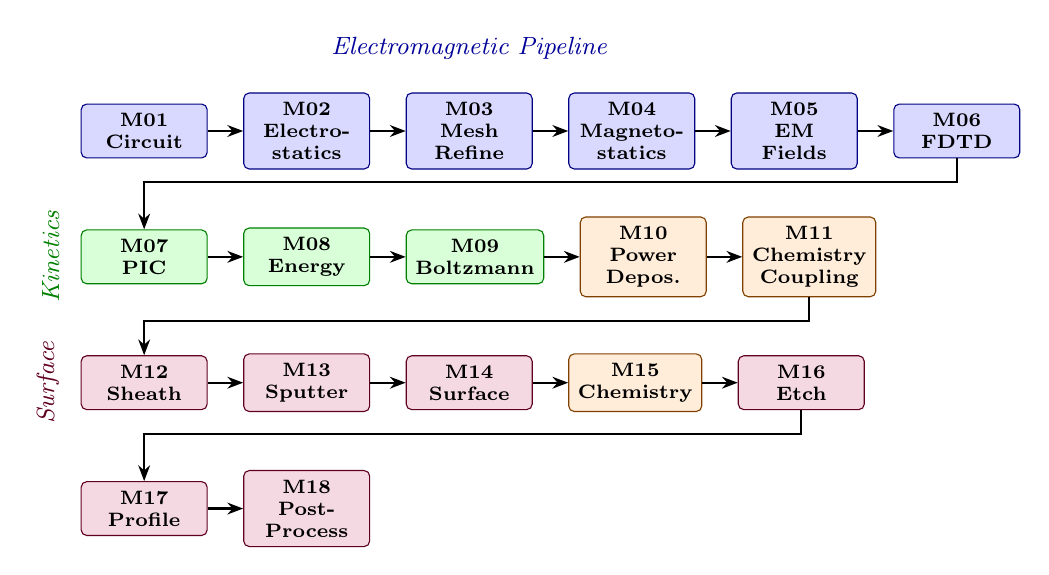
\begin{tikzpicture}[node distance=0.45cm,
    modbox/.style={rectangle, draw, rounded corners=2pt, minimum width=1.6cm, minimum height=0.65cm, align=center, font=\scriptsize\bfseries},
    embox/.style={modbox, fill=blue!15, draw=blue!50!black},
    picbox/.style={modbox, fill=green!15, draw=green!50!black},
    chembox/.style={modbox, fill=orange!15, draw=orange!50!black},
    surfbox/.style={modbox, fill=purple!15, draw=purple!50!black},
    arr/.style={-{Stealth[length=2mm]}, thick}]
    % Row 1: EM modules
    \node[embox] (m01) {M01\\Circuit};
    \node[embox, right=of m01] (m02) {M02\\Electro-\\statics};
    \node[embox, right=of m02] (m03) {M03\\Mesh\\Refine};
    \node[embox, right=of m03] (m04) {M04\\Magneto-\\statics};
    \node[embox, right=of m04] (m05) {M05\\EM\\Fields};
    \node[embox, right=of m05] (m06) {M06\\FDTD};
    % Row 2: Particle, Boltzmann, Power, Chemistry
    \node[picbox, below=0.9cm of m01] (m07) {M07\\PIC};
    \node[picbox, right=of m07] (m08) {M08\\Energy};
    \node[picbox, right=of m08] (m09) {M09\\Boltzmann};
    \node[chembox, right=of m09] (m10) {M10\\Power\\Depos.};
    \node[chembox, right=of m10] (m11) {M11\\Chemistry\\Coupling};
    % Row 3: Sheath, Surface, Etch
    \node[surfbox, below=0.9cm of m07] (m12) {M12\\Sheath};
    \node[surfbox, right=of m12] (m13) {M13\\Sputter};
    \node[surfbox, right=of m13] (m14) {M14\\Surface};
    \node[chembox, right=of m14] (m15) {M15\\Chemistry};
    \node[surfbox, right=of m15] (m16) {M16\\Etch};
    % Row 3 continued
    \node[surfbox, below=0.9cm of m12] (m17) {M17\\Profile};
    \node[surfbox, right=of m17] (m18) {M18\\Post-\\Process};
    % Arrows
    \draw[arr] (m01) -- (m02); \draw[arr] (m02) -- (m03);
    \draw[arr] (m03) -- (m04); \draw[arr] (m04) -- (m05);
    \draw[arr] (m05) -- (m06);
    \draw[arr] (m06.south) -- ++(0,-0.3) -| (m07.north);
    \draw[arr] (m07) -- (m08); \draw[arr] (m08) -- (m09);
    \draw[arr] (m09) -- (m10); \draw[arr] (m10) -- (m11);
    \draw[arr] (m11.south) -- ++(0,-0.3) -| (m12.north);
    \draw[arr] (m12) -- (m13); \draw[arr] (m13) -- (m14);
    \draw[arr] (m14) -- (m15); \draw[arr] (m15) -- (m16);
    \draw[arr] (m16.south) -- ++(0,-0.3) -| (m17.north);
    \draw[arr] (m17) -- (m18);
    % Labels
    \node[above=0.3cm of m03, font=\small\itshape, blue!60!black] {Electromagnetic Pipeline};
    \node[left=0.15cm of m07, font=\small\itshape, green!50!black, rotate=90, anchor=south] {Kinetics};
    \node[left=0.15cm of m12, font=\small\itshape, purple!50!black, rotate=90, anchor=south] {Surface};
  \end{tikzpicture}
  \caption{Architecture of the DTPM modular pipeline.  Configuration parameters are read from a YAML file and parsed into a \texttt{SimulationConfig} object.  Each module \texttt{M01}--\texttt{M18} receives the accumulated state dictionary and the configuration, performs its computation, and returns a dictionary of results that is merged into the state for downstream modules.  Modules are color-coded by functional group: blue for electromagnetic field solvers, green for particle kinetics, orange for chemistry and fluid coupling, and purple for surface and etch profile modules.}
  \label{fig:dtpm-architecture}
\end{figure}

\subsection{TEL ICP Reactor Configuration}

The target reactor is a TEL (Tokyo Electron Limited) ICP etcher configured for SF$_6$/Ar plasma etching of silicon wafers.  The reactor has a T-shaped geometry consisting of three sub-volumes:

\begin{itemize}
  \item \textbf{ICP source region:} A cylindrical quartz tube with inner radius $R_\mathrm{ICP} = \SI{38}{\milli\meter}$ and length $L_\mathrm{ICP} = \SI{150}{\milli\meter}$.  The RF coil (10 turns) is wound around the outside of this tube.
  \item \textbf{Processing chamber:} A larger cylindrical volume with radius $R_\mathrm{proc} = \SI{105}{\milli\meter}$ and length $L_\mathrm{proc} = \SI{50}{\milli\meter}$, housing the 6-inch (\SI{152}{\milli\meter}) silicon wafer on an electrostatic chuck.
  \item \textbf{Aperture:} A narrow connecting region of height $L_\mathrm{apt} = \SI{2}{\milli\meter}$ between the ICP source and the processing chamber, through which plasma and radicals diffuse.
\end{itemize}

The RF system provides dual-frequency power:
\begin{itemize}
  \item High-frequency (HF) source: $f_\mathrm{HF} = \SI{40}{\mega\hertz}$, $P_\mathrm{HF} = \SI{700}{\watt}$, driving the ICP coil for plasma generation.
  \item Low-frequency (LF) bias: $f_\mathrm{LF} = \SI{13}{\mega\hertz}$, $P_\mathrm{LF} = \SI{700}{\watt}$, applied to the wafer chuck for ion energy control.
\end{itemize}

The default computational mesh uses $50 \times 80$ grid points in the $(r, z)$ plane, of which 1669 cells lie within the active (gas-filled) domain and the remaining 2331 cells are masked as solid walls.  Grid spacings are $\dr = R_\mathrm{proc}/N_r$ and $\dz = (L_\mathrm{proc} + L_\mathrm{apt} + L_\mathrm{ICP})/N_z$.

\subsection{Module Descriptions}

Table~\ref{tab:module-descriptions} provides a brief description of each DTPM module and its role in the simulation pipeline.  The present work focuses on modules M01--M11, which together provide self-consistent electromagnetic field computation, power deposition, and plasma chemistry coupling.

\begin{longtable}{clp{8.5cm}}
\caption{DTPM module descriptions and status.} \label{tab:module-descriptions} \\
\toprule
\textbf{Module} & \textbf{Name} & \textbf{Description} \\
\midrule
\endfirsthead
\toprule
\textbf{Module} & \textbf{Name} & \textbf{Description} \\
\midrule
\endhead
M01 & RF Circuit        & Compute peak voltage, current, angular frequency from power, impedance, and frequency \\
M02 & Electrostatics    & Solve Laplace equation for electrostatic potential via SOR with Red-Black ordering \\
M03 & Mesh Refinement   & Gradient-based adaptive mesh refinement (disabled in the present work) \\
M04 & Magnetostatics    & Axisymmetric magnetic field from circular coils via elliptic integrals \\
M05 & EM Fields         & FDTD initialization from static solutions with sinusoidal RF source \\
M06 & FDTD              & Full FDTD electromagnetic solver with Mur ABC and Gaussian-modulated source \\
M06c & Cylindrical FDTD & TE-mode axisymmetric FDTD for $E_\theta$ in the ICP geometry \\
M07 & PIC Kinetics      & 2D3V Particle-in-Cell with Boris pusher and CIC deposition \\
M08 & Energy Analysis   & EEDF computation, mean $T_e$, energy conservation, heating profile \\
M09 & Boltzmann Solver  & Two-term spherical harmonic expansion with optional PINN surrogate \\
M10 & Power Deposition  & Ohmic heating $P(r,z) = \frac{1}{2}\sigma|E_\theta|^2$ from FDTD fields \\
M11 & Chemistry Coupling & Picard iteration coupling EM, $T_e$, $n_e$, and neutral transport \\
M12 & Sheath Model      & Collisionless sheath structure and ion energy distribution (future) \\
M13 & Sputtering        & Physical and chemical sputtering yields (future) \\
M14 & Surface Chemistry & Heterogeneous surface reaction kinetics (future) \\
M15 & Gas-Phase Chemistry & Detailed reaction mechanism integration (future) \\
M16 & Etch Rate         & Local etch rate from radical flux and ion bombardment (future) \\
M17 & Profile Evolution & Level-set or string method for feature-scale etch profile (future) \\
M18 & Post-Processing   & Diagnostics, data export, and surrogate-model training data (future) \\
\bottomrule
\end{longtable}


%=============================================================================
\chapter{Electromagnetic Field Computation}
\label{ch:em}
%=============================================================================

%======================================================================
\section{RF Circuit Analysis}
\label{sec:m01}
%======================================================================

The first module in the DTPM pipeline computes the fundamental RF electrical parameters that serve as boundary conditions for all downstream electromagnetic solvers.  For a matched RF source delivering power $P$ into a load impedance $Z$, the root-mean-square voltage is
\begin{equation}
  V_\mathrm{rms} = \sqrt{P \, Z}.
  \label{eq:m01-vrms}
\end{equation}
This expression assumes perfect impedance matching between the generator, the matching network, and the plasma load, which is a standard assumption in ICP modeling~\cite{Lieberman2005}.  The peak voltage and current follow from the sinusoidal waveform assumption:
\begin{align}
  V_\mathrm{peak} &= V_\mathrm{rms}\,\sqrt{2}, \label{eq:m01-vpeak}\\
  I_\mathrm{rms}  &= \frac{V_\mathrm{rms}}{Z}, \label{eq:m01-irms}\\
  I_\mathrm{peak} &= I_\mathrm{rms}\,\sqrt{2}, \label{eq:m01-ipeak}\\
  \omega          &= 2\pi f. \label{eq:m01-omega}
\end{align}

For a more detailed circuit model that includes the self-inductance and stray capacitance of the coil assembly, the module also provides an RLC impedance calculation.  The external circuit is modeled as a series RLC network, where $R$ is the coil resistance, $L$ is the coil inductance, and $C$ is the stray capacitance.  Kirchhoff's voltage law gives the complex impedance
\begin{equation}
  Z_\mathrm{ext} = R + j\!\left(\omega L - \frac{1}{\omega C}\right),
  \label{eq:m01-rlc}
\end{equation}
and the complex current is $I = V_\mathrm{applied} / Z_\mathrm{ext}$.  At resonance ($\omega L = 1/\omega C$), the impedance is purely resistive and the current is maximized.  The quality factor $Q = \omega L / R$ determines the bandwidth of the resonance.

In the default operating mode, M01 uses the simplified matched-load model of Eqs.~\eqref{eq:m01-vrms}--\eqref{eq:m01-omega}, which is appropriate when the matching network is tuned and the reflected power is negligible.  The RLC model becomes important when studying matching transients or off-resonance operation, which are outside the scope of the present work.

\begin{table}[htbp]
  \centering
  \caption{Default RF circuit parameters and computed M01 outputs for the TEL ICP reactor configuration.}
  \label{tab:m01-params}
  \begin{tabular}{@{}lll@{}}
    \toprule
    \textbf{Parameter} & \textbf{Symbol} & \textbf{Value} \\
    \midrule
    Source power        & $P$             & \SI{700}{\watt} \\
    Source frequency    & $f$             & \SI{40}{\mega\hertz} \\
    Load impedance      & $Z$             & \SI{50}{\ohm} \\
    \midrule
    RMS voltage         & $V_\mathrm{rms}$  & \SI{187.08}{\volt} \\
    Peak voltage        & $V_\mathrm{peak}$ & \SI{264.58}{\volt} \\
    RMS current         & $I_\mathrm{rms}$  & \SI{3.742}{\ampere} \\
    Peak current        & $I_\mathrm{peak}$ & \SI{5.292}{\ampere} \\
    Angular frequency   & $\omega$        & \SI{2.513e8}{\radian\per\second} \\
    \bottomrule
  \end{tabular}
\end{table}

The analytical verification is straightforward:
\begin{align}
  V_\mathrm{rms}  &= \sqrt{700 \times 50} = \SI{187.08}{\volt}, \\
  V_\mathrm{peak} &= 187.08 \times \sqrt{2} = \SI{264.58}{\volt}, \\
  I_\mathrm{peak} &= \frac{187.08}{50} \times \sqrt{2} = \SI{5.292}{\ampere}, \\
  \omega          &= 2\pi \times 40 \times 10^6 = \SI{2.513e8}{\radian\per\second}.
\end{align}
These values match the code output to all displayed digits, providing exact analytical validation of M01.

Module M01 is intentionally simple: its role is to translate user-facing engineering parameters (power, frequency, impedance) into physical quantities ($V_\mathrm{peak}$, $I_\mathrm{peak}$, $\omega$) that downstream modules consume directly.  The peak coil current $I_\mathrm{peak}$ enters the magnetostatic computation and the FDTD source term, while $V_\mathrm{peak}$ sets the Dirichlet boundary condition for the electrostatic solver (M02).


%======================================================================
\section{Electrostatic Field Solver}
\label{sec:m02}
%======================================================================

\subsection{Governing Equation and Boundary Conditions}

In the absence of free charge (a valid assumption for the vacuum electrostatic initialization), the electrostatic potential $\Phi(x,y)$ inside the reactor satisfies the Laplace equation
\begin{equation}
  \nabla^2 \Phi = \frac{\partial^2 \Phi}{\partial x^2}
                + \frac{\partial^2 \Phi}{\partial y^2} = 0.
  \label{eq:m02-laplace}
\end{equation}
Dirichlet boundary conditions are imposed on the coil cross-sections ($\Phi = V_\mathrm{peak}$) and on the grounded reactor walls ($\Phi = 0$).  Each coil is represented as a circular region in the $(r,z)$ plane with radius $a_\mathrm{coil} = \SI{2}{\milli\meter}$; grid points $(i,j)$ satisfying $(i - i_c)^2 + (j - j_c)^2 \le a_\mathrm{idx}^2$ are clamped to $V_\mathrm{peak}$, where $(i_c, j_c)$ is the coil center index and $a_\mathrm{idx}$ is the coil radius in grid units.

The Laplace equation with these mixed boundary conditions determines the vacuum electrostatic field that would exist if the coils were energized but no plasma were present.  This serves as the initial condition and electrostatic contribution to the combined field in downstream modules.

\subsection{Successive Over-Relaxation with Red-Black Ordering}

Equation~\eqref{eq:m02-laplace} is discretized on a uniform grid using standard second-order central finite differences:
\begin{equation}
  \frac{\Phi_{i+1,j} - 2\Phi_{i,j} + \Phi_{i-1,j}}{\dx^2}
  + \frac{\Phi_{i,j+1} - 2\Phi_{i,j} + \Phi_{i,j-1}}{\dy^2}
  = 0.
  \label{eq:m02-fd-laplace}
\end{equation}
For the equispaced grid ($\dx = \dy = h$), the Gauss--Seidel update becomes
\begin{equation}
  \Phi_{i,j}^{(k+1)} = \frac{1}{4}\!\left(
    \Phi_{i+1,j}^{(k)} + \Phi_{i-1,j}^{(k+1)}
    + \Phi_{i,j+1}^{(k)} + \Phi_{i,j-1}^{(k+1)}
  \right),
  \label{eq:m02-gs}
\end{equation}
where superscripts denote the iteration index and the asymmetry between $k$ and $k+1$ reflects the use of already-updated values.  Successive Over-Relaxation (SOR) accelerates convergence by introducing a relaxation parameter $\omega_\mathrm{SOR} \in (1, 2)$:
\begin{equation}
  \Phi_{i,j}^{(k+1)} = (1 - \omega_\mathrm{SOR})\,\Phi_{i,j}^{(k)}
  + \frac{\omega_\mathrm{SOR}}{4}\!\left(
    \Phi_{i+1,j} + \Phi_{i-1,j}
    + \Phi_{i,j+1} + \Phi_{i,j-1}
  \right).
  \label{eq:m02-sor}
\end{equation}

The optimal relaxation parameter for a rectangular domain with $N$ grid points in each direction is approximately~\cite{Press2007}
\begin{equation}
  \omega_\mathrm{opt} = \frac{2}{1 + \sin(\pi / N)} \approx 2 - \frac{2\pi}{N}.
  \label{eq:m02-omega-opt}
\end{equation}
In practice, the DTPM uses $\omega_\mathrm{SOR} = 1.8$, which is close to optimal for the $321 \times 221$ grid and provides robust convergence across different mesh resolutions.

The DTPM implementation uses \emph{Red-Black} (checkerboard) ordering to enable vectorized array operations.  The grid is partitioned into ``red'' points where $i + j$ is even and ``black'' points where $i + j$ is odd.  Within each half-sweep, all updates are independent and can be executed as a single NumPy array operation:
\begin{enumerate}
  \item Compute the neighbor average over the full grid using \texttt{np.roll}.
  \item Apply the SOR update~\eqref{eq:m02-sor} only at red (then black) free points via boolean masking.
  \item Restore fixed-potential points (coils and boundaries) from the stored initial values.
\end{enumerate}
This vectorization achieves a $50$--$100\times$ speedup over scalar Python loops while maintaining identical convergence behavior.

\subsection{Convergence Criterion}

The iteration terminates when the maximum residual falls below a user-specified tolerance:
\begin{equation}
  \max_{(i,j)\,\in\,\text{free}}\!
  \left|\Phi_{i,j}^{(k+1)} - \Phi_{i,j}^{(k)}\right|
  < \varepsilon,
  \label{eq:m02-convergence}
\end{equation}
with default tolerance $\varepsilon = 10^{-2}$.  For the $321 \times 221$ grid with $\omega_\mathrm{SOR} = 1.8$, convergence is achieved in approximately 2000 iterations.  The convergence rate is geometric with spectral radius
\begin{equation}
  \rho_\mathrm{SOR} = \omega_\mathrm{SOR} - 1 \approx 0.8,
\end{equation}
which means the residual decreases by a factor of $\sim 5$ every 10 iterations.

\subsection{Electric Field Computation}

Once the potential has converged, the electric field is obtained from $\mathbf{E} = -\nabla\Phi$ using second-order central finite differences at interior points:
\begin{align}
  E_x(i,j) &= -\frac{\Phi_{i+1,j} - \Phi_{i-1,j}}{2\,\dx},
  \label{eq:m02-ex}\\
  E_y(i,j) &= -\frac{\Phi_{i,j+1} - \Phi_{i,j-1}}{2\,\dy}.
  \label{eq:m02-ey}
\end{align}
At domain boundaries, one-sided first-order differences are used:
\begin{equation}
  E_x(0,j) = -\frac{\Phi_{1,j} - \Phi_{0,j}}{\dx}, \qquad
  E_x(N_x{-}1,j) = -\frac{\Phi_{N_x-1,j} - \Phi_{N_x-2,j}}{\dx},
  \label{eq:m02-ex-boundary}
\end{equation}
with analogous expressions for $E_y$ at $j = 0$ and $j = N_y - 1$.  The field magnitude is
\begin{equation}
  |\mathbf{E}| = \sqrt{E_x^2 + E_y^2}.
  \label{eq:m02-emag}
\end{equation}
The peak electric field of $|\mathbf{E}|_\mathrm{max} = \SI{4.14e4}{\volt\per\meter}$ occurs at the coil edges, consistent with the sharp potential gradient from $V_\mathrm{peak}$ to the surrounding grounded region.

\textbf{Implementation note.}  An early version of the code used forward differences $E_x \approx -(\Phi_{i+1,j} - \Phi_{i,j})/\dx$, which introduced a systematic half-grid-cell offset and reduced the accuracy to first order.  This was corrected to the central-difference stencil of Eqs.~\eqref{eq:m02-ex}--\eqref{eq:m02-ey} during the DTPM migration from legacy code.


%======================================================================
\section{Mesh Refinement}
\label{sec:m03}
%======================================================================

Accurate resolution of steep field gradients near coil windings and chamber walls demands finer spatial discretization than the bulk plasma region requires.  Module M03 implements an optional, gradient-based adaptive mesh refinement (AMR) pass that can be activated by setting \texttt{mesh\_refinement.enabled = True} in the YAML configuration file.

\subsection{Gradient-Based Flagging Criterion}

Given the electrostatic potential field $\Phi(r,z)$ computed by the Laplace solver (M02), the local gradient magnitude is evaluated on every cell:
\begin{equation}
  G_{i,j} = |\nabla\Phi|_{i,j}
          = \sqrt{\left(\frac{\partial\Phi}{\partial r}\right)^{\!2}
                 +\left(\frac{\partial\Phi}{\partial z}\right)^{\!2}}\,.
  \label{eq:amr-gradient}
\end{equation}
A cell is flagged for refinement whenever
\begin{equation}
  G_{i,j} > \mu_G + \sigma_\mathrm{thresh}\,\sigma_G,
  \label{eq:amr-flag}
\end{equation}
where $\mu_G$ and $\sigma_G$ are the mean and standard deviation of $G$ over the entire grid, and $\sigma_\mathrm{thresh}$ is a user-defined threshold (default 1.5).  This statistical criterion automatically identifies regions of high field gradient---typically near coil cross-sections and at geometric discontinuities---without requiring manual specification of refinement regions.

\subsection{Uniform Refinement and Interpolation}

Flagged patches are refined by a factor of 2 in each coordinate direction, producing local mesh spacing of $h/2$.  The coarse-grid solution is prolongated onto the refined patch via bilinear interpolation using \texttt{scipy.interpolate.RegularGridInterpolator}.  Boundary values of the refined patch are pinned to the coarse-grid solution, and the Laplace solver is re-run on the patch alone, producing a high-resolution correction at modest computational cost.

Because the refinement is optional and self-contained, downstream modules receive either the original or the refined field arrays transparently through the shared state dictionary.

\subsection{Status in the Present Work}

Mesh refinement is \textbf{disabled} in the present work.  The default $50 \times 80$ mesh for the TEL reactor geometry provides adequate resolution for the plasma chemistry coupling, and the cylindrical FDTD solver uses its own mesh generation that is independent of the Cartesian AMR.  The AMR capability is retained for future use with higher-resolution Cartesian simulations where field gradients near coils require sub-millimeter resolution.


%======================================================================
\section{Magnetostatic Field Solver}
\label{sec:m04}
%======================================================================

\subsection{Axisymmetric Solution via Elliptic Integrals}

Each ICP coil carries a peak current $I_\mathrm{peak}$ and is modeled as a circular loop of radius $a$ located at axial position $z_c$.  The magnetic field of a single circular loop is expressed exactly in terms of the complete elliptic integrals of the first and second kind, $K(k^2)$ and $E(k^2)$, following the treatment of Jackson~\cite{Jackson1998}, Section~5.5.

The Biot--Savart law for a single circular current loop gives, after integration over the azimuthal angle $\phi'$:
\begin{equation}
  d\mathbf{B} = \frac{\mu_0 I}{4\pi} \,
  \frac{d\mathbf{l} \times \hat{\mathbf{r}}'}{|\mathbf{r}'|^2},
  \label{eq:m04-biot-savart}
\end{equation}
where $\mathbf{r}' = \mathbf{r} - \mathbf{r}_\mathrm{source}$ is the displacement from the current element to the field point.  The current element on a loop of radius $a$ centered at axial position $z_c$ is parameterized as $d\mathbf{l} = a\,d\phi'\,(-\sin\phi'\,\hat{\mathbf{x}} + \cos\phi'\,\hat{\mathbf{y}})$, and the displacement vector is
\begin{equation}
  \mathbf{r}' = (r - a\cos\phi')\,\hat{\mathbf{x}} - a\sin\phi'\,\hat{\mathbf{y}} + (z - z_c)\,\hat{\mathbf{z}},
\end{equation}
with magnitude $|\mathbf{r}'|^2 = r^2 + a^2 - 2ar\cos\phi' + (z-z_c)^2$.

\subsection{Closed-Form Field Components}

Define the modulus parameter
\begin{equation}
  k^2 = \frac{4\,a\,r}{(a + r)^2 + (z - z_c)^2},
  \label{eq:m04-ksq}
\end{equation}
and the shorthand $\Delta z = z - z_c$.  After evaluating the cross product and integrating over $\phi' \in [0, 2\pi]$, the integrals reduce to combinations of the complete elliptic integrals
\begin{align}
  K(k^2) &= \int_0^{\pi/2} \frac{d\theta}{\sqrt{1 - k^2 \sin^2\theta}},
  \label{eq:m04-ellipk} \\
  E(k^2) &= \int_0^{\pi/2} \sqrt{1 - k^2 \sin^2\theta}\;d\theta,
  \label{eq:m04-ellipe}
\end{align}
yielding the exact axial field component
\begin{equation}
  \boxed{
  B_z(r,z) = \frac{\mu_0 I}{2\pi} \,
  \frac{1}{\sqrt{(a+r)^2 + \Delta z^2}} \left[
    K(k^2) + \frac{a^2 - r^2 - \Delta z^2}{(a-r)^2 + \Delta z^2}\,E(k^2)
  \right],}
  \label{eq:m04-bz}
\end{equation}
and the radial component
\begin{equation}
  \boxed{
  B_r(r,z) = \frac{\mu_0 I}{2\pi} \,
  \frac{\Delta z}{r\,\sqrt{(a+r)^2 + \Delta z^2}} \left[
    -K(k^2) + \frac{a^2 + r^2 + \Delta z^2}{(a-r)^2 + \Delta z^2}\,E(k^2)
  \right].}
  \label{eq:m04-br}
\end{equation}

These expressions are exact and numerically stable for all field points except those very close to the wire ($r \approx a$, $\Delta z \approx 0$) and on the axis ($r = 0$), both of which require special treatment described below.

\subsection{On-Axis Simplification}

At $r = 0$, the modulus $k^2 = 0$, so $K(0) = E(0) = \pi/2$, and Eq.~\eqref{eq:m04-bz} reduces to the textbook result for the field on the axis of a circular loop:
\begin{equation}
  B_z(0, z) = \frac{\mu_0\,I\,a^2}{2\,(a^2 + \Delta z^2)^{3/2}}.
  \label{eq:m04-bz-axis}
\end{equation}
Meanwhile $B_r(0,z) = 0$ by symmetry.  This closed-form result serves as a critical verification target for the numerical implementation: the code output matches Eq.~\eqref{eq:m04-bz-axis} to machine precision (relative error $< 10^{-14}$) at all grid points along the axis.

\subsection{Singularity Handling}

Two types of singularities require careful treatment:
\begin{enumerate}
  \item \emph{At the wire} ($r = a$, $\Delta z = 0$): the modulus $k^2 \to 1$ and $K(k^2) \to \infty$ logarithmically.  The implementation clamps $k^2 \le 1 - 10^{-12}$ and regularizes the denominator $(a-r)^2 + \Delta z^2$ by imposing a floor of $(0.01\,\dx)^2$.
  \item \emph{On axis} ($r = 0$): the factor $1/r$ in $B_r$ is singular.  Grid points with $r < 0.5\,\dx$ are flagged as ``on-axis'' and evaluated using the exact formula~\eqref{eq:m04-bz-axis} for $B_z$ and $B_r = 0$.
\end{enumerate}

\subsection{Superposition from Multiple Coils}

The total magnetic field is obtained by linear superposition over all $N_\mathrm{coils}$ individual loops:
\begin{equation}
  B_r^\mathrm{total}(r,z) = \sum_{c=1}^{N_\mathrm{coils}} B_r^{(c)}(r,z), \qquad
  B_z^\mathrm{total}(r,z) = \sum_{c=1}^{N_\mathrm{coils}} B_z^{(c)}(r,z),
  \label{eq:m04-superposition}
\end{equation}
where the sum runs over all coil loops.  In the default TEL configuration with 10 coil turns, each turn contributes independently to the total field.  The field magnitude $|\mathbf{B}| = \sqrt{B_r^2 + B_z^2}$ peaks at $|\mathbf{B}|_\mathrm{max} \approx \SI{8e-3}{\tesla}$ near the coil windings.

The computation is fully vectorized: for each coil, the arrays $R$, $Z$, $k^2$, $K(k^2)$, and $E(k^2)$ are evaluated over the entire $(N_r \times N_z)$ grid simultaneously using NumPy broadcasting and SciPy's \texttt{ellipk}/\texttt{ellipe} functions.  The legacy code (v6/DTPM) used a 36-segment discrete Biot--Savart summation with an \emph{ad hoc} projection onto 2D, which has been replaced entirely by the exact elliptic-integral solution.

\textbf{Advantage over discrete Biot--Savart.}  The elliptic-integral approach is both more accurate and faster than a segmented line-current approximation.  The segmented approach requires $N_\mathrm{seg}$ evaluations per coil (typically 36--360) and introduces discretization error proportional to $1/N_\mathrm{seg}^2$, whereas the elliptic-integral solution is exact to machine precision everywhere except at the regularized singularity points.


%======================================================================
\section{FDTD Electromagnetic Simulation}
\label{sec:m05m06}
%======================================================================

Modules M05 and M06 evolve the electromagnetic fields in time using the Finite-Difference Time-Domain (FDTD) method~\cite{Taflove2005,Yee1966}.  M05 initializes from the static solutions (M02 potential and M04 magnetic field) and drives the system with the RF source current.  M06 performs a standalone FDTD simulation with a Gaussian-modulated sinusoidal source for studying wave propagation.

\subsection{Maxwell's Equations in TM Mode}

In two spatial dimensions, the transverse-magnetic (TM) polarization retains three field components: $E_z$, $H_x$, and $H_y$.  Maxwell's curl equations reduce to
\begin{align}
  \frac{\partial H_x}{\partial t} &= -\frac{1}{\mu_0}\,
    \frac{\partial E_z}{\partial y},
    \label{eq:fdtd-hx} \\[4pt]
  \frac{\partial H_y}{\partial t} &= +\frac{1}{\mu_0}\,
    \frac{\partial E_z}{\partial x},
    \label{eq:fdtd-hy} \\[4pt]
  \frac{\partial E_z}{\partial t} &= \frac{1}{\varepsilon_0}\!\left(
    \frac{\partial H_y}{\partial x} - \frac{\partial H_x}{\partial y}
  \right) + J_\mathrm{source}.
    \label{eq:fdtd-ez}
\end{align}
These equations describe the propagation of electromagnetic waves in the reactor cavity and capture the RF field distribution generated by the coil current.

\subsection{Yee Grid Staggering}

Following Yee~\cite{Yee1966}, the electric and magnetic field components are staggered in both space and time.  On the 2D grid, $E_z$ is located at integer grid points $(i,j)$, $H_x$ is located at $(i, j+\frac{1}{2})$, and $H_y$ is located at $(i+\frac{1}{2}, j)$.  Temporal staggering places $\mathbf{H}$ at half-integer time steps $n + \frac{1}{2}$ relative to $\mathbf{E}$ at integer steps $n$.

This staggering scheme has several important properties:
\begin{itemize}
  \item It provides second-order accuracy in both space and time.
  \item The discrete curl operators are consistent with the continuum curl equations, ensuring that $\nabla \cdot \mathbf{B} = 0$ is satisfied to machine precision.
  \item The scheme is non-dissipative: in the absence of sources and losses, the discrete electromagnetic energy is exactly conserved.
\end{itemize}

\subsection{Leapfrog Time Update}

The leapfrog time-stepping scheme updates $\mathbf{H}$ at half time steps and $\mathbf{E}$ at integer time steps:
\begin{align}
  H_x^{n+1/2}\!\big|_{i,\,j+1/2} &= H_x^{n-1/2}\!\big|_{i,\,j+1/2}
    - \frac{\dt}{\mu_0\,\dy}\!\left(
      E_z^n\big|_{i,\,j+1} - E_z^n\big|_{i,\,j}\right),
    \label{eq:fdtd-hx-update} \\[4pt]
  H_y^{n+1/2}\!\big|_{i+1/2,\,j} &= H_y^{n-1/2}\!\big|_{i+1/2,\,j}
    + \frac{\dt}{\mu_0\,\dx}\!\left(
      E_z^n\big|_{i+1,\,j} - E_z^n\big|_{i,\,j}\right),
    \label{eq:fdtd-hy-update} \\[4pt]
  E_z^{n+1}\!\big|_{i,\,j} &= E_z^n\big|_{i,\,j}
    + \frac{\dt}{\varepsilon_0}\!\left(
      \frac{H_y^{n+1/2}\big|_{i+1/2,j} - H_y^{n+1/2}\big|_{i-1/2,j}}{\dx}
    - \frac{H_x^{n+1/2}\big|_{i,j+1/2} - H_x^{n+1/2}\big|_{i,j-1/2}}{\dy}
    \right).
    \label{eq:fdtd-ez-update}
\end{align}

\subsection{CFL Stability Condition}

The explicit leapfrog scheme is conditionally stable.  In 2D, the Courant--Friedrichs--Lewy (CFL) condition requires
\begin{equation}
  \dt \le \frac{1}{c\,\sqrt{\dfrac{1}{\dx^2} + \dfrac{1}{\dy^2}}}
  = \frac{\min(\dx, \dy)}{c\,\sqrt{2}} \quad\text{(for } \dx = \dy\text{)},
  \label{eq:fdtd-cfl}
\end{equation}
where $c = 1/\sqrt{\mu_0\varepsilon_0} = \SI{3e8}{\meter\per\second}$ is the speed of light.  The DTPM implementation uses a CFL factor of 0.5:
\begin{equation}
  \dt = 0.5 \times \frac{\min(\dx, \dy)}{c},
  \label{eq:fdtd-dt}
\end{equation}
which provides a safety margin well within the stability bound.  For $\dx = \SI{1}{\milli\meter}$, this yields $\dt \approx \SI{1.67e-12}{\second}$.  One RF cycle at \SI{40}{\mega\hertz} requires $T_\mathrm{RF}/\dt \approx 15000$ time steps.

\subsection{Mur First-Order Absorbing Boundary Conditions}

Open boundaries are treated with Mur's first-order absorbing boundary condition (ABC)~\cite{Mur1981}, derived from the one-dimensional advection equation $\partial E_z / \partial t + c\,\partial E_z / \partial x = 0$ at the boundary $x = 0$.  Discretizing this one-way wave equation in a manner consistent with the FDTD staggering yields the Mur update formula:
\begin{equation}
  \boxed{
  E_z^{n+1}\big|_0 = E_z^{n}\big|_1
    + \frac{c\,\dt - \dx}{c\,\dt + \dx}
    \left(E_z^{n+1}\big|_1 - E_z^{n}\big|_0\right).}
  \label{eq:mur-abc}
\end{equation}
Analogous expressions apply at $x = N_x - 1$ and at both $y$ boundaries.  The coefficient $(c\,\dt - \dx)/(c\,\dt + \dx)$ is precomputed once and stored.  For the default CFL factor of 0.5, this coefficient equals $-1/3$, which provides effective attenuation of outgoing waves without significant spurious reflection.

The Mur ABC is first-order accurate and provides approximately 20--30~dB of reflection suppression for waves at normal incidence.  For waves at oblique incidence, the reflection coefficient increases, but this is acceptable for the present application where the primary concern is preventing wave reflections from contaminating the interior field pattern.

\subsection{Source Terms}

\paragraph{Sinusoidal RF source (M05).}  Module M05 initializes the magnetic field from the magnetostatic solution $\mathbf{H} = \mathbf{B}_s / \mu_0$ and drives $E_z$ with a sinusoidal current source distributed across the $N_\mathrm{coils}$ coil positions:
\begin{equation}
  E_z^{n+1}\big|_{i_c,j_c} \mathrel{+}= \frac{I_\mathrm{peak}}{N_\mathrm{coils}}
  \sin(\omega\,n\,\dt),
  \label{eq:m05-source}
\end{equation}
where $(i_c, j_c)$ are the grid indices of coil $c$.

\paragraph{Gaussian-modulated source (M06).}  Module M06 uses a Gaussian-modulated sinusoidal (soft) source that provides a smooth turn-on and finite bandwidth:
\begin{equation}
  S(t) = \sin(\omega\,t)\;\exp\!\left[-\left(\frac{t - t_0}{\tau}\right)^{\!2}\right],
  \label{eq:m06-source}
\end{equation}
where $t_0 = 1.5\,T_\mathrm{RF}$ centers the envelope and $\tau = 0.5\,T_\mathrm{RF}$ controls the pulse width.  The smooth turn-on avoids the high-frequency transients that would result from an abrupt sinusoidal start.

\subsection{Energy Diagnostics}

Both modules track the total electromagnetic energy as a stability diagnostic:
\begin{equation}
  U_\mathrm{EM} = \frac{1}{2}\,\varepsilon_0 \sum_{i,j} E_z^2\,\dx\,\dy
              + \frac{1}{2}\,\mu_0 \sum_{i,j}\!\left(H_x^2 + H_y^2\right)\dx\,\dy.
  \label{eq:fdtd-energy}
\end{equation}
In the absence of sources and absorbing boundaries, $U_\mathrm{EM}$ is conserved to machine precision, confirming the symplecticity of the leapfrog scheme.  When the source is active, the energy grows monotonically as RF power is injected into the domain.


%=============================================================================
\chapter{Particle Kinetics and Energy Analysis}
\label{ch:kinetics}
%=============================================================================

%======================================================================
\section{Particle-in-Cell Method}
\label{sec:m07}
%======================================================================

Module M07 implements a 2D3V electrostatic Particle-in-Cell (PIC) scheme~\cite{Birdsall2004,Hockney1988} to simulate the kinetic behavior of electrons and ions under the combined electromagnetic fields computed by M02--M06.  The ``2D3V'' designation means two-dimensional spatial positions $(x, y)$ with three-dimensional velocities $(v_x, v_y, v_z)$, which is necessary to capture gyration about the in-plane magnetic field.

\subsection{Cloud-in-Cell Charge Deposition}

Each macroparticle with charge $q_p$ at position $(x_p, y_p)$ deposits charge onto the four nearest grid nodes using bilinear (Cloud-in-Cell, CIC) weighting.  Let
\begin{equation}
  i = \left\lfloor \frac{x_p}{\dx} - \frac{1}{2} \right\rfloor, \qquad
  j = \left\lfloor \frac{y_p}{\dy} - \frac{1}{2} \right\rfloor,
  \label{eq:pic-cell-index}
\end{equation}
and define the fractional displacements
\begin{equation}
  w_x = \frac{x_p}{\dx} - \frac{1}{2} - i, \qquad
  w_y = \frac{y_p}{\dy} - \frac{1}{2} - j.
  \label{eq:pic-weights}
\end{equation}
Then the charge density contribution at the four surrounding nodes is
\begin{align}
  \rho(i,j)         &\mathrel{+}= \frac{q_p}{\dx\,\dy}\,(1 - w_x)(1 - w_y),
  \label{eq:cic-deposit-00}\\
  \rho(i{+}1,j)     &\mathrel{+}= \frac{q_p}{\dx\,\dy}\,w_x\,(1 - w_y),
  \label{eq:cic-deposit-10}\\
  \rho(i,j{+}1)     &\mathrel{+}= \frac{q_p}{\dx\,\dy}\,(1 - w_x)\,w_y,
  \label{eq:cic-deposit-01}\\
  \rho(i{+}1,j{+}1) &\mathrel{+}= \frac{q_p}{\dx\,\dy}\,w_x\,w_y.
  \label{eq:cic-deposit-11}
\end{align}
The implementation uses NumPy's \texttt{add.at} for the scatter operation, which correctly handles multiple particles contributing to the same cell without race conditions.

\subsection{Self-Consistent Poisson Solve via FFT}

The self-consistent space-charge electric field is obtained by solving the Poisson equation
\begin{equation}
  \nabla^2 \phi = -\frac{\rho}{\varepsilon_0}
  \label{eq:poisson}
\end{equation}
on the periodic domain using a spectral method.  In Fourier space,
\begin{equation}
  \hat{\phi}(\mathbf{k}) = \frac{\hat{\rho}(\mathbf{k})}
    {-\varepsilon_0\,(k_x^2 + k_y^2)},
  \label{eq:poisson-fourier}
\end{equation}
with $\hat{\phi}(\mathbf{0}) = 0$ to fix the zero-mean gauge.  The electric field is then
\begin{equation}
  E_\alpha = -\mathcal{F}^{-1}\!\left[i\,k_\alpha\,\hat{\phi}\right], \qquad
  \alpha \in \{x, y\}.
  \label{eq:poisson-efield}
\end{equation}
The 2D real-valued FFT (\texttt{rfft2}) reduces the computational cost to $\mathcal{O}(N \log N)$ per Poisson solve, where $N = N_x \times N_y$.

\subsection{Cloud-in-Cell Field Gathering}

The inverse operation gathers field values at particle positions using the same bilinear weights as deposition:
\begin{equation}
  F_p = F(i,j)\,(1{-}w_x)(1{-}w_y) + F(i{+}1,j)\,w_x(1{-}w_y)
      + F(i,j{+}1)\,(1{-}w_x)w_y + F(i{+}1,j{+}1)\,w_x\,w_y.
  \label{eq:cic-gather}
\end{equation}
Using the same weights for both deposition and gathering ensures momentum conservation (the scheme is self-adjoint), which is essential for long-time stability of the PIC simulation.

\subsection{Boris Leap-Frog Pusher}

The Boris algorithm~\cite{Boris1970,Birdsall2004} advances particle velocities under the Lorentz force $\mathbf{F} = q(\mathbf{E} + \mathbf{v} \times \mathbf{B})$ in a way that exactly preserves energy in a pure magnetic field.  The algorithm proceeds in four steps.

\paragraph{Step 1: Half electric kick.}  Accelerate by the electric field for half a time step:
\begin{equation}
  \mathbf{v}^- = \mathbf{v}^n + \frac{q\,\dt}{2m}\,\mathbf{E}.
  \label{eq:boris-halfkick1}
\end{equation}

\paragraph{Step 2: Magnetic rotation.}  Define the rotation vectors
\begin{equation}
  \mathbf{t} = \frac{q\,\dt}{2m}\,\mathbf{B}, \qquad
  \mathbf{s} = \frac{2\,\mathbf{t}}{1 + |\mathbf{t}|^2}.
  \label{eq:boris-ts}
\end{equation}
Compute the intermediate velocity
\begin{equation}
  \mathbf{v}' = \mathbf{v}^- + \mathbf{v}^- \times \mathbf{t},
  \label{eq:boris-vprime}
\end{equation}
then apply the rotation:
\begin{equation}
  \mathbf{v}^+ = \mathbf{v}^- + \mathbf{v}' \times \mathbf{s}.
  \label{eq:boris-vplus}
\end{equation}
The key property is that $|\mathbf{v}^+| = |\mathbf{v}^-|$: the magnetic rotation preserves the kinetic energy exactly, regardless of the time step.  This is because the transformation $\mathbf{v}^- \to \mathbf{v}^+$ is an exact rotation in the Cayley--Hamilton sense, with determinant equal to unity.

In 2D3V, the cross products expand to
\begin{align}
  v'_x &= v^-_x + v^-_y\,t_z - v^-_z\,t_y, \\
  v'_y &= v^-_y + v^-_z\,t_x - v^-_x\,t_z, \\
  v'_z &= v^-_z + v^-_x\,t_y - v^-_y\,t_x,
\end{align}
and similarly for $\mathbf{v}^+ = \mathbf{v}^- + \mathbf{v}' \times \mathbf{s}$.  The full 3D magnetic field $(B_x, B_y, B_z)$ participates in the rotation, enabling correct Larmor gyration for arbitrary field orientations.

\paragraph{Step 3: Second half electric kick.}
\begin{equation}
  \mathbf{v}^{n+1} = \mathbf{v}^+ + \frac{q\,\dt}{2m}\,\mathbf{E}.
  \label{eq:boris-halfkick2}
\end{equation}

\paragraph{Step 4: Position update.}
\begin{equation}
  \mathbf{x}^{n+1} = \mathbf{x}^n + \mathbf{v}^{n+1}\,\dt.
  \label{eq:boris-xupdate}
\end{equation}
In 2D3V, the velocity has three components $(v_x, v_y, v_z)$ while the position update uses only the in-plane components $(v_x, v_y)$.

\subsection{Reflecting Boundary Conditions}

In the default mode (appropriate for the bounded ICP reactor cavity), particles hitting a wall undergo specular reflection: the normal velocity component is reversed and the position is mirrored about the wall plane:
\begin{align}
  v_\perp &\leftarrow -v_\perp, \\
  x &\leftarrow 2\,x_\mathrm{wall} - x.
\end{align}
Periodic and absorbing boundary conditions are also supported but not used in the present work.

\subsection{Particle Initialization}

Electrons and ions are initialized with positions uniformly distributed over the domain and velocities drawn from a Maxwellian distribution:
\begin{equation}
  v_\alpha \sim \mathcal{N}\!\left(0,\; v_\mathrm{th}\right), \qquad
  v_\mathrm{th} = \sqrt{\frac{e\,T_e[\mathrm{eV}]}{m}},
  \label{eq:pic-maxwellian}
\end{equation}
for each velocity component $\alpha \in \{x, y, z\}$.

\subsection{Validation}

The Boris pusher was subjected to three canonical test problems:
\begin{itemize}
  \item \textbf{Larmor gyration:} A single electron in $B_z = \SI{0.01}{\tesla}$ with $v_\perp = \SI{1e6}{\meter\per\second}$.  After 1000 gyro-periods, the Larmor radius error is $3.9 \times 10^{-7}$ (relative) and kinetic energy is conserved with relative error $4 \times 10^{-15}$ (machine precision).
  \item \textbf{$\mathbf{E} \times \mathbf{B}$ drift:} Crossed fields $E_x = \SI{100}{\volt\per\meter}$, $B_z = \SI{0.01}{\tesla}$.  Drift velocity error: $2.5 \times 10^{-5}$ relative over 100 gyro-periods.
  \item \textbf{Full PIC simulation:} 5000 electron + 5000 ion macroparticles, 200 PIC steps, $\dt = \SI{1e-10}{\second}$, reflecting boundaries.
\end{itemize}


%======================================================================
\section{Energy Analysis}
\label{sec:m08}
%======================================================================

Module M08 post-processes the particle data from M07 to extract key energy diagnostics that characterize the electron population and power coupling.

\subsection{Electron Energy Distribution Function}

The EEDF is computed by histogramming the kinetic energies of the electron macroparticles:
\begin{equation}
  \varepsilon_p = \frac{1}{2}\,m_e\!\left(v_{x,p}^2 + v_{y,p}^2 + v_{z,p}^2\right),
  \label{eq:eedf-energy}
\end{equation}
converted to electron-volts via $\varepsilon_p[\mathrm{eV}] = \varepsilon_p / e$.  The distribution $f(\varepsilon)$ is obtained by binning these energies into $N_\mathrm{bin} = 100$ uniformly spaced bins over $[0, \varepsilon_\mathrm{max}]$ and normalizing to unit area:
\begin{equation}
  \int_0^{\varepsilon_\mathrm{max}} f(\varepsilon)\;d\varepsilon = 1.
  \label{eq:eedf-norm}
\end{equation}
For a Maxwellian plasma, the EEDF takes the form $f(\varepsilon) \propto \sqrt{\varepsilon}\,\exp(-\varepsilon / k_B T_e)$.  Deviations from this shape (high-energy tails, bi-Maxwellian structure) indicate non-equilibrium conditions characteristic of ICP discharges at low pressure~\cite{Lieberman2005}.

\subsection{Mean Electron Temperature}

The mean electron temperature is computed from the average kinetic energy via the equipartition theorem for three degrees of freedom:
\begin{equation}
  T_e = \frac{2}{3}\langle\varepsilon\rangle
      = \frac{2}{3} \times \frac{1}{N_p}\sum_{p=1}^{N_p} \varepsilon_p[\mathrm{eV}]
  \qquad [\mathrm{eV}].
  \label{eq:m08-te}
\end{equation}
The factor $2/3$ arises because each degree of freedom contributes $\frac{1}{2} k_B T_e$ to the average energy, so $\langle\varepsilon\rangle = \frac{3}{2} k_B T_e$.

\subsection{Energy Conservation Check}

The change in total kinetic energy should equal the cumulative work done by the electric field on the particles:
\begin{equation}
  \Delta \mathrm{KE} = \mathrm{KE}_{N_t} - \mathrm{KE}_0
  \stackrel{!}{=} \sum_{n=0}^{N_t - 1} \left(\sum_p q_p\,\mathbf{E}_p \cdot \mathbf{v}_p\right) \dt
  = \int \mathbf{E} \cdot \mathbf{J}\;dV\;dt.
  \label{eq:m08-energy-conservation}
\end{equation}
The relative error $|\Delta\mathrm{KE} - W_\mathrm{total}| / |W_\mathrm{total}|$ is logged at the end of each simulation.  For pure magnetic gyration (no $\mathbf{E}$), the Boris pusher preserves kinetic energy to machine precision ($\sim 10^{-15}$ relative error).

\subsection{Spatially Resolved Heating Rate}

The spatial distribution of electron heating is computed by evaluating the power absorbed per particle and depositing it onto the grid using the same CIC weights:
\begin{equation}
  P(i,j) = \frac{1}{\dx\,\dy} \sum_{p \in \mathrm{cell}(i,j)}
    q_p\!\left(E_{x,p}\,v_{x,p} + E_{y,p}\,v_{y,p}\right).
  \label{eq:m08-heating}
\end{equation}
This provides the spatially resolved Ohmic heating profile $P(r,z)\;[\si{\watt\per\meter\cubed}]$, which is a critical input for the power balance and fluid equations in downstream modules.  The heating profile peaks near the coil locations where the induced electric field is strongest, and decays exponentially into the plasma bulk with a characteristic skin depth $\delta \sim c/\omega_\mathrm{pe}$, where $\omega_\mathrm{pe} = \sqrt{n_e e^2/(m_e \varepsilon_0)}$ is the electron plasma frequency.


%======================================================================
\section{Boltzmann Solver}
\label{sec:m09}
%======================================================================

Accurate electron transport coefficients and rate coefficients for inelastic processes require knowledge of the EEDF, which in general departs significantly from a Maxwellian.  Module M09 solves the electron Boltzmann equation under the two-term spherical-harmonic expansion and, optionally, replaces the conventional numerical solver with a physics-informed neural network (PINN) surrogate.

\subsection{Two-Term Spherical Harmonic Expansion}

In the two-term approximation, the distribution is written $f(\varepsilon,\hat{\mathbf{v}}) = f_0(\varepsilon) + f_1(\varepsilon)\cos\theta$, where $\varepsilon$ is the electron energy.  The isotropic part satisfies the Boltzmann equation~\cite{Hagelaar2005}
\begin{equation}
  \frac{\partial f_0}{\partial\varepsilon}
  = -\frac{1}{3\varepsilon}\,\frac{d}{d\varepsilon}
    \!\left[\varepsilon^2\,\nu_m(\varepsilon)\,\frac{df_0}{d\varepsilon}\right]
  + \sum_j C_j[f_0],
  \label{eq:bte-twoterm}
\end{equation}
where $\nu_m(\varepsilon)$ is the momentum-transfer collision frequency and $C_j[f_0]$ are the inelastic collision operators (excitation, ionization, attachment) for process $j$.  The equation is discretized on a uniform energy grid and solved as a tridiagonal system.

Once $f_0(\varepsilon)$ is known, transport and rate coefficients are computed as energy-weighted integrals:
\begin{align}
  \mu_e &= -\frac{e}{3m_e}\int_0^\infty
          \frac{\varepsilon}{\nu_m(\varepsilon)}\,
          \frac{df_0}{d\varepsilon}\,d\varepsilon,
  \label{eq:mobility} \\
  k_j   &= \sqrt{\frac{2}{m_e}}\int_0^\infty
          \varepsilon\,\sigma_j(\varepsilon)\,f_0(\varepsilon)\,d\varepsilon.
  \label{eq:rate-coeff}
\end{align}

\subsection{PINN Surrogate Architecture}

When PINN mode is enabled~\cite{Raissi2019,Kim2023}, a multilayer perceptron (MLP) is trained to predict $f_0(\varepsilon)$ given the reduced electric field $E/N$ as input.  The network architecture consists of 4 hidden layers with 128 neurons each, using $\tanh$ activation functions.  The loss function combines a physics-informed PDE residual with boundary and normalization constraints:
\begin{equation}
  \mathcal{L} = \mathcal{L}_\mathrm{PDE}
              + \lambda_1\,\mathcal{L}_\mathrm{norm}
              + \lambda_2\,\mathcal{L}_\mathrm{BC},
  \label{eq:pinn-loss}
\end{equation}
where $\mathcal{L}_\mathrm{PDE}$ penalizes violations of Eq.~\eqref{eq:bte-twoterm} at collocation points, $\mathcal{L}_\mathrm{norm}$ enforces the normalization condition $\int f_0\,d\varepsilon = 1$, and $\mathcal{L}_\mathrm{BC}$ enforces the boundary conditions $f_0(0) = \mathrm{finite}$ and $f_0(\varepsilon_\mathrm{max}) = 0$.  The penalty weights $\lambda_1$ and $\lambda_2$ are tuned via hyperparameter optimization.

The trained PINN surrogate provides a continuous, differentiable representation of $f_0(\varepsilon; E/N)$ that can be evaluated at arbitrary energy and field values without re-solving the Boltzmann equation, enabling rapid parameter sweeps and real-time coupling with the FDTD solver.

\textbf{Status in the present work.}  Module M09 is implemented but not yet activated in the self-consistent coupling loop.  The present work uses Maxwellian EEDF assumptions for rate coefficients, with the Boltzmann solver reserved for future validation studies.


%=============================================================================
\newpage
\chapter{SF$_6$/Ar Plasma Chemistry}
\label{part:chemistry}
%=============================================================================


%======================================================================
\section{Zero-Dimensional Global Model}
\label{sec:0d-model}
%======================================================================

The plasma chemistry in the DTPM is built upon a zero-dimensional (0D) global model that provides the fundamental balance equations relating electron temperature, electron density, and species concentrations.  The 0D model serves two roles: (i) as a standalone tool for exploring chemistry over broad parameter ranges, and (ii) as the initial-guess generator for the 2D self-consistent iteration in the present work.

\subsection{Reactor Geometry}

The reactor geometry is encapsulated in a \texttt{Reactor} class that computes all derived geometric quantities from the primary dimensions:
\begin{align}
  V &= \pi R^2 L, \qquad A_\mathrm{ax} = 2\pi R^2, \qquad A_\mathrm{rad} = 2\pi RL, \\
  A &= A_\mathrm{ax} + A_\mathrm{rad}, \qquad
  \Lambda = \left[\left(\frac{\pi}{L}\right)^2 + \left(\frac{2.405}{R}\right)^2\right]^{-1/2},
  \label{eq:reactor-geometry}
\end{align}
where $R$ is the reactor radius, $L$ is the height, $V$ is the volume, $A$ is the total wall area, and $\Lambda$ is the effective diffusion length.  The factor 2.405 is the first zero of the Bessel function $J_0$, arising from the fundamental diffusion mode in a cylinder.

For the Lallement reactor~\cite{Lallement2009}: $R = \SI{0.180}{\meter}$, $L = \SI{0.175}{\meter}$, giving $V = \SI{0.0178}{\meter\cubed}$, $A = \SI{0.402}{\meter\cubed}$, and $\Lambda = \SI{0.049}{\meter}$.

For the TEL etcher (the target reactor of the present work): $R_\mathrm{ICP} = \SI{0.038}{\meter}$, $L_\mathrm{ICP} = \SI{0.150}{\meter}$, with a separate processing chamber below.

\subsection{Species Inventory}

The model tracks 26 species in total:
\begin{itemize}
  \item \textbf{Neutrals (9):} $\SFsix$, $\SFfive$, $\SFfour$, $\SFthree$, SF$_2$, SF, S, F, F$_2$.
  \item \textbf{Positive ions (8):} SF$_5^+$, SF$_4^+$, SF$_3^+$, SF$_2^+$, SF$^+$, S$^+$, F$^+$, Ar$^+$.
  \item \textbf{Negative ions (7):} SF$_6^-$, SF$_5^-$, SF$_4^-$, SF$_3^-$, SF$_2^-$, F$^-$, F$_2^-$.
  \item \textbf{Argon species (3):} Ar (ground state), Ar$^+$ (ion), Ar$^*$ (${}^3P_2$ metastable at \SI{11.55}{\electronvolt}).
  \item \textbf{Electrons.}
\end{itemize}

\subsection{Particle Balance for Electron Temperature}

The electron temperature $\Te$ is determined by the steady-state particle balance: the total ionization rate must equal the total loss rate (attachment plus wall losses):
\begin{equation}
  \boxed{R_\mathrm{iz}(\Te) + \frac{R_\mathrm{Penn}}{n_e} = R_\mathrm{att}(\Te) + k_w^+(\Te,\alpha)(1+\alpha),}
  \label{eq:Te-balance}
\end{equation}
where $R_\mathrm{iz}$ is the total electron-impact ionization rate coefficient summed over all channels and neutral targets, $R_\mathrm{att}$ is the total dissociative attachment rate coefficient, $R_\mathrm{Penn}/n_e$ is the Penning ionization contribution from Ar$^*$, and $k_w^+(1+\alpha)$ is the ion wall loss rate including the electronegativity correction.  This equation is solved for $\Te$ using the Brent root-finding method  on the interval $[0.5, 15]\eV$.

\subsection{Power Balance for Electron Density}

Once $\Te$ is known, the electron density follows from the power balance:
\begin{equation}
  \boxed{P_\mathrm{abs} = n_e\, R_\mathrm{iz}\, \varepsilon_T\, e\, V,}
  \label{eq:power-balance}
\end{equation}
where $P_\mathrm{abs} = \eta P_\mathrm{rf}$ is the absorbed power, $e$ is the elementary charge, $V$ is the reactor volume, and $\varepsilon_T$ is the total energy cost per electron--ion pair:
\begin{equation}
  \varepsilon_T = \varepsilon_c + \varepsilon_{iw} + 2\Te,
  \label{eq:eps-T}
\end{equation}
with collisional energy loss
\begin{equation}
  \varepsilon_c = \frac{\sum_j \sum_k E_k\, k_{kj}\, n_j}{R_\mathrm{iz,total}},
  \label{eq:Ec}
\end{equation}
ion wall energy $\varepsilon_{iw} = \frac{1}{2}\Te \ln(M_i / 2\pi m_e)$, and electron wall energy $\varepsilon_{ew} = 2\Te$.

\subsection{Electronegativity}

The electronegativity parameter $\alpha = n_-/n_e$ is determined by combining the negative ion balance with charge neutrality ($n_+ = n_e + n_- = n_e(1+\alpha)$):
\begin{equation}
  \boxed{\alpha(1+\alpha) = \frac{R_\mathrm{att}}{k_\mathrm{rec}\,n_e},}
  \label{eq:alpha-quadratic}
\end{equation}
where $k_\mathrm{rec} = \SI{1.5e-9}{\centi\meter\cubed\per\second}$ is the ion--ion recombination rate coefficient.  The physical root is
\begin{equation}
  \alpha = \frac{-1 + \sqrt{1 + 4\,R_\mathrm{att}/(k_\mathrm{rec}\,n_e)}}{2}.
  \label{eq:alpha-solution}
\end{equation}

\subsection{Ar$^*$ Metastable Balance}

The Ar$^*$ density is determined by the balance between electron-impact excitation and all quenching and ionization channels:
\begin{equation}
  n_{\Ar^*} = \frac{k_{\Ar,\mathrm{exc}}\, n_e\, n_\Ar}{(k_{\Ar,\mathrm{iz,m}} + k_{\Ar,q})n_e + k_{w,\Ar^*} + R_\mathrm{quench,heavy}},
  \label{eq:Ar-star}
\end{equation}
where $R_\mathrm{quench,heavy}$ includes Penning ionization ($k_\mathrm{Penn} = \SI{2e-10}{\centi\meter\cubed\per\second}$, Velazco and Setser~\cite{Velazco1975}) and non-ionizing quenching by all molecular species ($k_\mathrm{qnch} = \SI{3e-10}{\centi\meter\cubed\per\second}$).

\subsection{Ion Wall Loss}

The ion wall loss rate follows the Lee--Lieberman formulation~\cite{Lee1995} for electronegative plasmas with the Kim \emph{h}-factor model~\cite{Kim2006}:
\begin{equation}
  k_w^+ = u_B \left( \frac{2\,h_L\,A_\mathrm{ax} + h_R\,A_\mathrm{rad}}{V}\right),
  \label{eq:ion-wall-loss}
\end{equation}
where the modified Bohm velocity incorporating electronegativity is
\begin{equation}
  u_B = \sqrt{\frac{e\Te(1+\alpha)}{M_i(1+\gamma\alpha)}}, \qquad \gamma = \frac{\Te}{T_-},
  \label{eq:Bohm-EN}
\end{equation}
and the \emph{h}-factors use the quadratic two-term ansatz $h = \sqrt{h_a^2 + h_c^2}$, where $h_a$ is the parabolic-profile term and $h_c$ provides a physically necessary floor at high electronegativity.  The electronegativity correction factor is
\begin{equation}
  \mathrm{EN} = \frac{1 + 3\alpha/\gamma}{1 + \alpha}.
\end{equation}


%======================================================================
\section{54-Reaction Mechanism}
\label{sec:reaction-mechanism}
%======================================================================

The gas-phase chemistry follows the comprehensive 54-reaction mechanism of Lallement et al.~\cite{Lallement2009}, which provides a complete description of the SF$_6$/Ar plasma.  The reactions are organized into the categories listed in Table~\ref{tab:reactions}.

\begin{longtable}{clp{6cm}c}
\caption{Summary of the 54-reaction gas-phase mechanism.  Rate coefficient forms: A = Arrhenius ($k = A\exp(-E/\Te)$), T = Troe fall-off, C = constant.} \label{tab:reactions} \\
\toprule
\textbf{Cat.} & \textbf{Count} & \textbf{Description} & \textbf{Form} \\
\midrule
\endfirsthead
\toprule
\textbf{Cat.} & \textbf{Count} & \textbf{Description} & \textbf{Form} \\
\midrule
\endhead
D1--D5  & 5 & SF$_6$ electron-impact dissociation: e + SF$_6 \to$ SF$_x$ + (6$-x$)F & A \\
D6--D10 & 5 & Sequential SF$_x$ dissociation: e + SF$_x \to$ SF$_{x-1}$ + F & A \\
\midrule
I1--I7  & 7 & Dissociative ionization of SF$_6$: e + SF$_6 \to$ SF$_x^+$ + ... + 2e & A \\
I8--I12 & 5 & Ionization of fragments: e + SF$_x \to$ SF$_x^+$ + 2e & A \\
\midrule
A1--A7  & 7 & Dissociative attachment: e + SF$_6 \to$ SF$_x^-$ + F$_y$ & A \\
\midrule
R1--R3  & 3 & Troe fall-off recombination: F + SF$_x$ + M $\to$ SF$_{x+1}$ + M & T \\
R4--R6  & 3 & Disproportionation: SF$_x$ + SF$_y \to$ products & C \\
R7--R9  & 3 & Other neutral--neutral reactions & C \\
\midrule
N1      & 1 & Ion--ion recombination: A$^+$ + B$^- \to$ neutrals & C \\
\midrule
Ar1     & 1 & Ar direct ionization: e + Ar $\to$ Ar$^+$ + 2e & A \\
Ar2     & 1 & Ar excitation: e + Ar $\to$ Ar$^*$ + e & A \\
Ar3     & 1 & Stepwise ionization: e + Ar$^* \to$ Ar$^+$ + 2e & A \\
Ar4     & 1 & Superelastic quenching: e + Ar$^* \to$ Ar + e & A \\
Ar5     & 1 & Elastic scattering: e + Ar $\to$ Ar + e & A \\
\midrule
P1      & 1 & Penning ionization: Ar$^*$ + SF$_6 \to$ SF$_5^+$ + F + Ar + e & C \\
P2      & 1 & Quenching: Ar$^*$ + SF$_6 \to$ Ar + SF$_5$ + F & C \\
P3      & 1 & Metastable pooling: Ar$^*$ + Ar$^* \to$ Ar$^+$ + Ar + e & C \\
\bottomrule
\end{longtable}

\subsection{Electron-Impact Rate Coefficients}

All electron-impact rate coefficients use the Arrhenius-like parameterization fitted to Maxwellian-averaged cross sections:
\begin{equation}
  k(\Te) = A \exp\!\left(-\frac{E_\mathrm{th}}{\Te}\right) \quad [\text{cm}^3\,\text{s}^{-1}],
  \label{eq:arrhenius}
\end{equation}
where $\Te$ is the electron temperature in eV and $E_\mathrm{th}$ is the threshold energy.  An alternative five-parameter logarithmic form is used for some reactions:
\begin{equation}
  k(\Te) = \exp\!\left(A + B\ln \Te + \frac{C}{\Te} + \frac{D}{\Te^2} + \frac{E}{\Te^3}\right) \quad [\text{m}^3\,\text{s}^{-1}].
  \label{eq:druyvesteyn-rate}
\end{equation}

\subsection{Troe Fall-Off Recombination}

Three-body recombination of F with SF$_x$ fragments uses the Troe fall-off formula~\cite{Ryan1990}:
\begin{equation}
  \boxed{k_\mathrm{eff} = \frac{k_0[M]}{1 + P_r} \cdot F_c^{\left(1+\left[\log_{10}(P_r)\right]^2\right)^{-1}},}
  \label{eq:troe}
\end{equation}
where $P_r = k_0[M]/k_\infty$ is the reduced pressure, $k_0$ is the low-pressure limit rate coefficient, $k_\infty$ is the high-pressure limit, $[M]$ is the total gas density (bath gas), and $F_c$ is the broadening factor.

\begin{table}[H]
\centering
\caption{Troe fall-off parameters for neutral recombination reactions.}
\label{tab:troe}
\begin{tabular}{clcccc}
\toprule
& \textbf{Reaction} & $k_0$ (cm$^6$/s) & $k_\infty$ (cm$^3$/s) & $F_c$ & \textbf{Regime at 1\,Pa} \\
\midrule
R1 & F + SF$_5 \to$ SF$_6$ & $3.4\times10^{-23}$ & $1\times10^{-11}$ & 0.43 & High-$p$ limit \\
R2 & F + SF$_4 \to$ SF$_5$ & $3.7\times10^{-28}$ & $5\times10^{-12}$ & 0.46 & Low-$p$ limit \\
R3 & F + SF$_3 \to$ SF$_4$ & $2.8\times10^{-26}$ & $2\times10^{-11}$ & 0.47 & Fall-off \\
\bottomrule
\end{tabular}
\end{table}

The correct implementation of the Troe formula is critical at low pressures typical of ICP etchers ($p \sim 1$--\SI{10}{\milli\torr}).  Using the high-pressure limit $k_\infty$ instead of the full Troe expression overestimates the recombination rate by factors of 5--180 at \SI{10}{\milli\torr}, as the bath gas density $[M]$ is too low to stabilize the collision complex efficiently~\cite{Ryan1990}.

\subsection{Disproportionation Reactions}

Three disproportionation reactions convert SF$_x$ fragment pairs into more stable species:
\begin{align}
  \text{SF}_5 + \text{SF}_5 &\to \text{SF}_6 + \text{SF}_4, & k &= \SI{1.5e-11}{\centi\meter\cubed\per\second}, \\
  \text{F}_2 + \text{SF}_4 &\to \text{SF}_5 + \text{F},     & k &= \SI{8.3e-14}{\centi\meter\cubed\per\second}, \\
  \text{F}_2 + \text{SF}_3 &\to \text{SF}_4 + \text{F},     & k &= \SI{5.0e-14}{\centi\meter\cubed\per\second}.
\end{align}

\subsection{Ion--Ion Recombination}

All positive--negative ion pairs undergo mutual neutralization with a rate coefficient $k_{ii} = \SI{1.1e-7}{\centi\meter\cubed\per\second}$, which is a typical value for room-temperature ion--ion recombination in molecular gases.


%======================================================================
\section{Wall Surface Chemistry}
\label{sec:wall-chemistry}
%======================================================================

The wall surface chemistry model follows the framework of Kokkoris et al.~\cite{Kokkoris2009}, which describes the heterogeneous reactions at reactor walls through a 5-channel mechanism involving adsorption, fluorination, recombination, and desorption.

\subsection{Five-Channel Mechanism}

The wall reactions are parameterized by five probabilities:
\begin{enumerate}
  \item $s_\mathrm{F}$: F atom sticking (adsorption) probability on bare surface sites.
  \item $s_{\SFx}$: SF$_x$ radical sticking probability.
  \item $p_\mathrm{fluor}$: Probability of fluorination reaction (F attacking adsorbed SF$_x$).
  \item $p_\mathrm{wr}$: Probability of wall recombination (F + F$_\mathrm{(ads)} \to$ F$_2$).
  \item $p_\mathrm{FF}$: Eley--Rideal recombination probability.
\end{enumerate}

The surface coverage evolves according to
\begin{equation}
  \frac{d\theta_\mathrm{F}}{dt} = s_\mathrm{F}\,\frac{\bar{v}_\mathrm{F}}{4}\,\frac{A}{V\,n_\mathrm{sites}}\,n_\mathrm{F}\,(1 - \theta_\mathrm{F} - \theta_\mathrm{SFx}) - p_\mathrm{wr}\,\frac{\bar{v}_\mathrm{F}}{4}\,\frac{A}{V\,n_\mathrm{sites}}\,n_\mathrm{F}\,\theta_\mathrm{F},
\end{equation}
where $n_\mathrm{sites} = \SI{1e19}{\per\meter\squared}$ is the surface site density and $\bar{v}_\mathrm{F} = \sqrt{8k_BT_g/(\pi m_\mathrm{F})}$ is the mean thermal velocity of F atoms.

\subsection{Material-Specific Recombination Coefficients}

The effective wall recombination coefficient $\gamma$ varies by material:
\begin{table}[H]
\centering
\caption{Wall recombination coefficients for F atoms on reactor materials.}
\label{tab:gamma-values}
\begin{tabular}{lcl}
\toprule
\textbf{Material} & $\gamma$ & \textbf{Source} \\
\midrule
Quartz (SiO$_2$) & 0.001 & Kokkoris~\cite{Kokkoris2009} \\
Aluminum (Al)     & 0.18  & Calibrated to Mettler~\cite{Mettler2025} \\
Silicon wafer     & 0.025 & Kokkoris~\cite{Kokkoris2009} \\
Quartz window     & 0.001 & Same as quartz \\
\bottomrule
\end{tabular}
\end{table}

The aluminum recombination coefficient $\gamma_\mathrm{Al} = 0.18$ is the single calibrated parameter in the TEL reactor model, fitted to reproduce the experimentally observed $\sim 74\,\%$ centre-to-edge F density drop at the 90\,\%~SF$_6$ bias-off branch of Mettler Fig.~4.17~\cite{Mettler2025}.  (Note: Fig.~4.14 in Mettler's dissertation is the normalised radial profile at 70~sccm~SF$_6$ / 30~sccm~Ar with 200~W wafer bias, distinct from the 90\%~SF$_6$ bias-off branch of Fig.~4.17.)  A cross-check against the 30\,\%~SF$_6$ branch (67\,\% drop) with the same $\gamma_\mathrm{Al}$ is reported in Section~\ref{sec:mettler-fig417-direct}.

\subsection{Robin Boundary Condition}

At the wall, the F atom flux into the surface equals the recombination loss:
\begin{equation}
  \boxed{-D_\mathrm{F}\,\frac{\partial n_\mathrm{F}}{\partial n} = \gamma\,\frac{\bar{v}_\mathrm{F}}{4}\,n_\mathrm{F},}
  \label{eq:robin-bc}
\end{equation}
where $\partial/\partial n$ is the outward normal derivative at the wall.  This Robin (mixed) boundary condition couples the diffusion coefficient $D_\mathrm{F}$ and the wall loss rate $\gamma\bar{v}/4$, providing a self-consistent treatment of wall chemistry that interpolates between the transport-limited regime ($\gamma \to 1$, $n_\mathrm{F}|_\mathrm{wall} \approx 0$) and the kinetics-limited regime ($\gamma \ll 1$, $n_\mathrm{F}|_\mathrm{wall} \approx n_\mathrm{F}|_\mathrm{bulk}$).

\subsection{SF$_6$ Regeneration}

Each F atom lost at the wall through recombination with adsorbed SF$_x$ fragments regenerates SF$_6$ at a rate
\begin{equation}
  R_\mathrm{regen} = \gamma_\mathrm{regen}\,\frac{\bar{v}_\mathrm{F}}{4}\,\frac{A}{V}\,n_\mathrm{F},
\end{equation}
where $\gamma_\mathrm{regen}$ accounts for the fraction of wall encounters that produce SF$_6$ rather than other products.  This regeneration pathway is important for maintaining the SF$_6$ feed gas density, particularly in reactors with large surface-to-volume ratios.


%======================================================================
\section{Complete Gas-Phase Reaction Tables}
\label{sec:reaction-tables}
%======================================================================

The full set of 49 electron-impact and heavy-particle gas-phase reactions implemented in the DTPM is tabulated below.  Table~\ref{tab:gas-reactions-1} lists the first 23 reactions, covering electron-impact dissociation of the parent gas and fragments, as well as dissociative and direct ionization channels.  Table~\ref{tab:gas-reactions-2} lists the remaining 26 reactions, including dissociative attachment, Troe-corrected neutral recombination, disproportionation, ion--ion neutralisation, argon electron-impact processes, and Penning channels.  All rate coefficients are expressed in the Arrhenius form $k = A\exp(-E_\mathrm{th}/T_e)$ unless otherwise noted; pre-exponential factors $A$ are given in cm$^3$\,s$^{-1}$ and threshold energies $E_\mathrm{th}$ in eV.

\begin{longtable}{@{}clcc@{}}
\caption{Gas-phase reaction set, Part~I: dissociation, fragment dissociation, dissociative ionisation, and fragment ionisation.  Rate coefficients use the Arrhenius form $k = A\exp(-E_\mathrm{th}/T_e)$ in cm$^3$\,s$^{-1}$.}
\label{tab:gas-reactions-1} \\
\toprule
\textbf{\#} & \textbf{Reaction} & $A$ \textbf{(cm$^3$/s)} & $E_\mathrm{th}$ \textbf{(eV)} \\
\midrule
\endfirsthead
\toprule
\textbf{\#} & \textbf{Reaction} & $A$ \textbf{(cm$^3$/s)} & $E_\mathrm{th}$ \textbf{(eV)} \\
\midrule
\endhead
\multicolumn{4}{@{}l}{\textit{Parent gas dissociation}} \\
G1  & $\mathrm{e} + \SFsix \to \SFfive + \mathrm{F} + \mathrm{e}$ & $1.5\times10^{-7}$ & 8.1 \\
G2  & $\mathrm{e} + \SFsix \to \SFfour + 2\mathrm{F} + \mathrm{e}$ & $9.0\times10^{-9}$ & 13.4 \\
G3  & $\mathrm{e} + \SFsix \to \SFthree + 3\mathrm{F} + \mathrm{e}$ & $2.5\times10^{-8}$ & 33.5 \\
G4  & $\mathrm{e} + \SFsix \to \mathrm{SF_2} + 2\mathrm{F} + \mathrm{F_2} + \mathrm{e}$ & $2.3\times10^{-8}$ & 23.9 \\
G5  & $\mathrm{e} + \SFsix \to \mathrm{SF} + 3\mathrm{F} + \mathrm{F_2} + \mathrm{e}$ & $1.5\times10^{-9}$ & 26.0 \\
\midrule
\multicolumn{4}{@{}l}{\textit{Fragment dissociation}} \\
G6  & $\mathrm{e} + \mathrm{F_2} \to 2\mathrm{F} + \mathrm{e}$ & $1.2\times10^{-8}$ & 5.8 \\
G7  & $\mathrm{e} + \SFfive \to \SFfour + \mathrm{F} + \mathrm{e}$ & $1.5\times10^{-7}$ & 9.0 \\
G8  & $\mathrm{e} + \SFfour \to \SFthree + \mathrm{F} + \mathrm{e}$ & $6.2\times10^{-8}$ & 9.0 \\
G9  & $\mathrm{e} + \SFthree \to \mathrm{SF_2} + \mathrm{F} + \mathrm{e}$ & $8.6\times10^{-8}$ & 9.0 \\
G10 & $\mathrm{e} + \mathrm{SF_2} \to \mathrm{SF} + \mathrm{F} + \mathrm{e}$ & $4.5\times10^{-8}$ & 9.0 \\
G11 & $\mathrm{e} + \mathrm{SF} \to \mathrm{S} + \mathrm{F} + \mathrm{e}$ & $6.2\times10^{-8}$ & 9.0 \\
\midrule
\multicolumn{4}{@{}l}{\textit{Dissociative ionisation of SF$_6$}} \\
G12 & $\mathrm{e} + \SFsix \to \SFfive^+ + \mathrm{F} + 2\mathrm{e}$ & $1.2\times10^{-7}$ & 18.1 \\
G13 & $\mathrm{e} + \SFsix \to \SFfour^+ + 2\mathrm{F} + 2\mathrm{e}$ & $8.4\times10^{-9}$ & 19.9 \\
G14 & $\mathrm{e} + \SFsix \to \SFthree^+ + 3\mathrm{F} + 2\mathrm{e}$ & $3.2\times10^{-8}$ & 20.7 \\
G15 & $\mathrm{e} + \SFsix \to \mathrm{SF_2^+} + 4\mathrm{F} + 2\mathrm{e}$ & $7.6\times10^{-9}$ & 24.4 \\
G16 & $\mathrm{e} + \SFsix \to \mathrm{SF^+} + 5\mathrm{F} + 2\mathrm{e}$ & $1.2\times10^{-8}$ & 26.0 \\
G17 & $\mathrm{e} + \SFsix \to \mathrm{S^+} + 6\mathrm{F} + 2\mathrm{e}$ & $1.4\times10^{-8}$ & 39.9 \\
G18 & $\mathrm{e} + \SFsix \to \mathrm{F^+} + \SFfive + 2\mathrm{e}$ & $1.2\times10^{-8}$ & 31.7 \\
\midrule
\multicolumn{4}{@{}l}{\textit{Direct ionisation of fragments}} \\
G19 & $\mathrm{e} + \SFfive \to \SFfive^+ + 2\mathrm{e}$ & $1.0\times10^{-7}$ & 17.8 \\
G20 & $\mathrm{e} + \SFfive \to \SFfour^+ + \mathrm{F} + 2\mathrm{e}$ & $9.4\times10^{-8}$ & 22.8 \\
G21 & $\mathrm{e} + \SFthree \to \SFthree^+ + 2\mathrm{e}$ & $1.0\times10^{-7}$ & 18.9 \\
G22 & $\mathrm{e} + \mathrm{F} \to \mathrm{F^+} + 2\mathrm{e}$ & $1.3\times10^{-8}$ & 16.5 \\
G23 & $\mathrm{e} + \mathrm{S} \to \mathrm{S^+} + 2\mathrm{e}$ & $1.6\times10^{-7}$ & 13.3 \\
\bottomrule
\end{longtable}

\begin{longtable}{@{}clc@{}}
\caption{Gas-phase reaction set, Part~II: dissociative attachment, Troe recombination, disproportionation, ion--ion neutralisation, Ar electron-impact processes, and Penning channels.  Rate forms: A = Arrhenius, P = power-law, T = Troe fall-off, C = constant.}
\label{tab:gas-reactions-2} \\
\toprule
\textbf{\#} & \textbf{Reaction} & $k$ \textbf{or functional form} \\
\midrule
\endfirsthead
\toprule
\textbf{\#} & \textbf{Reaction} & $k$ \textbf{or functional form} \\
\midrule
\endhead
\multicolumn{3}{@{}l}{\textit{Dissociative attachment}} \\
G24 & $\mathrm{e} + \SFsix \to \SFsix^- $ & $2.4\times10^{-10}\,T_e^{-1.49}$ \\
G25 & $\mathrm{e} + \SFsix \to \SFfive^- + \mathrm{F}$ & $2.0\times10^{-11}\,T_e^{-1.46}$ \\
G26 & $\mathrm{e} + \SFsix \to \SFfour^- + 2\mathrm{F}$ & $3.9\times10^{-12}\,e^{0.45T_e - 0.04T_e^2}$ \\
G27 & $\mathrm{e} + \SFsix \to \SFthree^- + 3\mathrm{F}$ & $1.2\times10^{-13}\,e^{0.70T_e - 0.05T_e^2}$ \\
G28 & $\mathrm{e} + \SFsix \to \mathrm{SF_2^-} + 4\mathrm{F}$ & $5.4\times10^{-15}\,e^{0.77T_e - 0.05T_e^2}$ \\
G29 & $\mathrm{e} + \SFsix \to \mathrm{F^-} + \SFfive$ & $3.4\times10^{-11}\,e^{0.46T_e - 0.04T_e^2}$ \\
G30 & $\mathrm{e} + \mathrm{F_2} \to \mathrm{F_2^-}$ & $2.2\times10^{-13}\,e^{0.71T_e - 0.05T_e^2}$ \\
\midrule
\multicolumn{3}{@{}l}{\textit{Troe fall-off neutral recombination (Ryan \& Plumb 1990)}} \\
G31 & $\mathrm{F} + \SFfive + \mathrm{M} \to \SFsix + \mathrm{M}$ & $k_0{=}3.4{\times}10^{-23}$,\; $k_\infty{=}1{\times}10^{-11}$,\; $F_c{=}0.43$ \\
G32 & $\mathrm{F} + \SFfour + \mathrm{M} \to \SFfive + \mathrm{M}$ & $k_0{=}3.7{\times}10^{-28}$,\; $k_\infty{=}5{\times}10^{-12}$,\; $F_c{=}0.46$ \\
G33 & $\mathrm{F} + \SFthree + \mathrm{M} \to \SFfour + \mathrm{M}$ & $k_0{=}2.8{\times}10^{-26}$,\; $k_\infty{=}2{\times}10^{-11}$,\; $F_c{=}0.47$ \\
G34 & $\mathrm{F} + \mathrm{SF_2} + \mathrm{M} \to \SFthree + \mathrm{M}$ & $k_0{=}1.7{\times}10^{-28}$,\; $k_\infty{=}2{\times}10^{-11}$,\; $F_c{=}0.56$ \\
G35 & $\mathrm{F} + \mathrm{SF} + \mathrm{M} \to \mathrm{SF_2} + \mathrm{M}$ & $k_0{=}1.0{\times}10^{-30}$,\; $k_\infty{=}2{\times}10^{-11}$,\; $F_c{=}0.67$ \\
G36 & $\mathrm{F} + \mathrm{S} + \mathrm{M} \to \mathrm{SF} + \mathrm{M}$ & $k_0{=}7.5{\times}10^{-33}$,\; $k_\infty{=}2{\times}10^{-11}$,\; $F_c{=}0.73$ \\
\midrule
\multicolumn{3}{@{}l}{\textit{Disproportionation}} \\
G37 & $\SFfive + \SFfive \to \SFsix + \SFfour$ & $2.5\times10^{-11}$\,cm$^3$/s \\
G38 & $\mathrm{F_2} + \SFfour \to \SFfive + \mathrm{F}$ & $2.5\times10^{-11}$\,cm$^3$/s \\
G39 & $\mathrm{F_2} + \SFthree \to \SFfour + \mathrm{F}$ & $2.5\times10^{-11}$\,cm$^3$/s \\
\midrule
\multicolumn{3}{@{}l}{\textit{Ion--ion neutralisation}} \\
G40 & $\mathrm{A^+} + \mathrm{B^-} \to \text{neutrals}$ & $1.5\times10^{-9}$\,cm$^3$/s \\
\midrule
\multicolumn{3}{@{}l}{\textit{Argon electron-impact reactions}} \\
G41 & $\mathrm{e} + \Ar \to \Ar^+ + 2\mathrm{e}$ & $1.2\times10^{-10}\,e^{-21.7/T_e}$ \\
G42 & $\mathrm{e} + \Ar \to \Ar^* + \mathrm{e}$ & $4.2\times10^{-9}\,e^{-8.0/T_e}$ \\
G43 & $\mathrm{e} + \Ar^* \to \Ar^+ + 2\mathrm{e}$ & $2.05\times10^{-7}\,e^{-4.95/T_e}$ \\
G44 & $\mathrm{e} + \Ar^* \to \Ar + \mathrm{e}$ & $2.0\times10^{-7}$ (const.) \\
\midrule
\multicolumn{3}{@{}l}{\textit{Penning ionisation and Ar$^*$ quenching}} \\
G45 & $\Ar^* + \SFsix \to \SFfive^+ + \mathrm{F} + \Ar + \mathrm{e}$ & $2.0\times10^{-10}$\,cm$^3$/s \\
G46 & $\Ar^* + \SFsix \to \Ar + \SFfive + \mathrm{F}$ & $3.0\times10^{-10}$\,cm$^3$/s \\
G47 & $\Ar^* + \SFx \to \Ar + \text{products}$ & $1.0\times10^{-10}$\,cm$^3$/s \\
G48 & $\Ar^* + \mathrm{F_2} \to \Ar + 2\mathrm{F}$ & $5.0\times10^{-11}$\,cm$^3$/s \\
G49 & $\Ar^* + \mathrm{F} \to \Ar + \mathrm{F}$ & $5.0\times10^{-12}$\,cm$^3$/s \\
\bottomrule
\end{longtable}


%======================================================================
\section{Complete Wall-Surface Reaction Mechanism}
\label{sec:wall-reactions-full}
%======================================================================

Table~\ref{tab:wall-reactions} lists the complete set of 40 heterogeneous wall-surface reactions implemented in the DTPM, following the five-channel framework of Kokkoris et al.~\cite{Kokkoris2009}.  The reactions are organised by mechanism category: adsorption and sticking (S1--S8), sequential fluorination (S9--S16), surface recombinations via the Eley--Rideal mechanism (S17--S24), ion--surface interactions (S25--S32), and deposition/desorption processes (S33--S40).

\begin{longtable}{@{}clp{5.5cm}c@{}}
\caption{Wall-surface reactions (S1--S40) after Kokkoris et al.\ (2009), Table~2.  Probability symbols: $s_\mathrm{F}$, $s_{\mathrm{SF}_x}$, $p_\mathrm{fluor}$, $p_\mathrm{wr}$, $p_\mathrm{FF}$.  Values are material-dependent (see Table~\ref{tab:surface-kinetics}).}
\label{tab:wall-reactions} \\
\toprule
\textbf{\#} & \textbf{Category} & \textbf{Reaction} & \textbf{Probability} \\
\midrule
\endfirsthead
\toprule
\textbf{\#} & \textbf{Category} & \textbf{Reaction} & \textbf{Probability} \\
\midrule
\endhead
S1  & Adsorption & $\mathrm{F(g)} \to \mathrm{F(ads)}$ on bare site       & $s_\mathrm{F}$ \\
S2  & Adsorption & $\SFfive\mathrm{(g)} \to \SFfive\mathrm{(ads)}$        & $s_{\mathrm{SF}_x}$ \\
S3  & Adsorption & $\SFfour\mathrm{(g)} \to \SFfour\mathrm{(ads)}$        & $s_{\mathrm{SF}_x}$ \\
S4  & Adsorption & $\SFthree\mathrm{(g)} \to \SFthree\mathrm{(ads)}$      & $s_{\mathrm{SF}_x}$ \\
S5  & Adsorption & $\mathrm{SF_2(g)} \to \mathrm{SF_2(ads)}$              & $s_{\mathrm{SF}_x}$ \\
S6  & Adsorption & $\mathrm{SF(g)} \to \mathrm{SF(ads)}$                  & $s_{\mathrm{SF}_x}$ \\
S7  & Adsorption & $\mathrm{S(g)} \to \mathrm{S(ads)}$                    & $s_{\mathrm{SF}_x}$ \\
S8  & Adsorption & $\mathrm{F_2(g)} \to \mathrm{F_2(ads)}$                & $s_{\mathrm{SF}_x}$ \\
\midrule
S9  & Fluorination & $\mathrm{F(g)} + \SFfive\mathrm{(ads)} \to \SFsix\mathrm{(g)}$   & $p_\mathrm{fluor}$ \\
S10 & Fluorination & $\mathrm{F(g)} + \SFfour\mathrm{(ads)} \to \SFfive\mathrm{(g)}$   & $p_\mathrm{fluor}$ \\
S11 & Fluorination & $\mathrm{F(g)} + \SFthree\mathrm{(ads)} \to \SFfour\mathrm{(g)}$  & $p_\mathrm{fluor}$ \\
S12 & Fluorination & $\mathrm{F(g)} + \mathrm{SF_2(ads)} \to \SFthree\mathrm{(g)}$     & $p_\mathrm{fluor}$ \\
S13 & Fluorination & $\mathrm{F(g)} + \mathrm{SF(ads)} \to \mathrm{SF_2(g)}$            & $p_\mathrm{fluor}$ \\
S14 & Fluorination & $\mathrm{F(g)} + \mathrm{S(ads)} \to \mathrm{SF(g)}$               & $p_\mathrm{fluor}$ \\
S15 & Fluorination & $\mathrm{F(g)} + \mathrm{F(ads)} \to \mathrm{F_2(g)}$              & $p_\mathrm{fluor}$ \\
S16 & Fluorination & $\mathrm{F(g)} + \mathrm{F_2(ads)} \to \mathrm{F_2(g)} + \mathrm{F(g)}$ & $p_\mathrm{fluor}$ \\
\midrule
S17 & Eley--Rideal & $\mathrm{F(g)} + \mathrm{F(ads)} \to \mathrm{F_2(g)}$         & $p_\mathrm{wr}$ \\
S18 & Eley--Rideal & $\SFfive\mathrm{(g)} + \mathrm{F(ads)} \to \SFsix\mathrm{(g)}$ & $p_\mathrm{wr}$ \\
S19 & Eley--Rideal & $\SFfour\mathrm{(g)} + \mathrm{F(ads)} \to \SFfive\mathrm{(g)}$ & $p_\mathrm{wr}$ \\
S20 & Eley--Rideal & $\SFthree\mathrm{(g)} + \mathrm{F(ads)} \to \SFfour\mathrm{(g)}$ & $p_\mathrm{wr}$ \\
S21 & Eley--Rideal & $\mathrm{SF_2(g)} + \mathrm{F(ads)} \to \SFthree\mathrm{(g)}$ & $p_\mathrm{wr}$ \\
S22 & Eley--Rideal & $\mathrm{SF(g)} + \mathrm{F(ads)} \to \mathrm{SF_2(g)}$       & $p_\mathrm{wr}$ \\
S23 & Eley--Rideal & $\mathrm{S(g)} + \mathrm{F(ads)} \to \mathrm{SF(g)}$          & $p_\mathrm{wr}$ \\
S24 & Eley--Rideal & $\mathrm{F_2(g)} + \mathrm{F(ads)} \to \mathrm{F_2(g)} + \mathrm{F(g)}$ & $p_\mathrm{wr}$ \\
\midrule
S25 & Ion--surface & $\SFfive^+ \to \SFfive\mathrm{(ads)}$ & $\sim1$ \\
S26 & Ion--surface & $\SFfour^+ \to \SFfour\mathrm{(ads)}$ & $\sim1$ \\
S27 & Ion--surface & $\SFthree^+ \to \SFthree\mathrm{(ads)}$ & $\sim1$ \\
S28 & Ion--surface & $\mathrm{SF_2^+} \to \mathrm{SF_2(ads)}$ & $\sim1$ \\
S29 & Ion--surface & $\mathrm{SF^+} \to \mathrm{SF(ads)}$ & $\sim1$ \\
S30 & Ion--surface & $\mathrm{S^+} \to \mathrm{S(ads)}$ & $\sim1$ \\
S31 & Ion--surface & $\mathrm{F^+} \to \mathrm{F(ads)}$ & $\sim1$ \\
S32 & Ion--surface & $\Ar^+ \to \Ar\mathrm{(g)}$ (reflected) & $\sim1$ \\
\midrule
S33 & Desorption & $\SFsix\mathrm{(ads)} \to \SFsix\mathrm{(g)}$ & thermal \\
S34 & Desorption & $\mathrm{F_2(ads)} \to \mathrm{F_2(g)}$ & thermal \\
S35 & Deposition & $\mathrm{S(ads)}$ accumulates on wall & --- \\
S36 & Deposition & $\mathrm{SF_2(ads)}$ accumulates on wall & --- \\
S37 & Deposition & $\mathrm{SF(ads)}$ accumulates on wall & --- \\
S38 & Sputtering & $\mathrm{ion} + \mathrm{deposit} \to \mathrm{products(g)}$ & $Y(E_i)$ \\
S39 & F$_2$ form. & $\mathrm{F(ads)} + \mathrm{F(ads)} \to \mathrm{F_2(g)}$ & $p_\mathrm{FF}$ \\
S40 & Net regen. & $\mathrm{F(g)} + \SFfive\mathrm{(ads)} \to \SFsix\mathrm{(g)}$ (net) & $p_\mathrm{fluor}$ \\
\bottomrule
\end{longtable}


%======================================================================
\section{Material-Specific Surface Kinetics}
\label{sec:surface-kinetics}
%======================================================================

Each wall material in the TEL reactor is characterised by a distinct set of the five surface-kinetics probabilities.  Table~\ref{tab:surface-kinetics} lists the values implemented in the DTPM, based on the Kokkoris et al.\ parameterisation~\cite{Kokkoris2009} with $\gamma_\mathrm{Al}$ calibrated to the Mettler radical probe data~\cite{Mettler2025}.

\begin{table}[H]
\centering
\caption{Material-specific surface kinetics parameters.  All values are dimensionless probabilities per gas--surface encounter.}
\label{tab:surface-kinetics}
\begin{tabular}{@{}lccccc@{}}
\toprule
\textbf{Material} & $s_\mathrm{F}$ & $s_{\mathrm{SF}_x}$ & $p_\mathrm{fluor}$ & $p_\mathrm{wr}$ & $p_\mathrm{FF}$ \\
\midrule
Quartz (SiO$_2$)   & 0.0015 & 0.0005 & 0.025  & 0.007  & 0.003 \\
Aluminium (Al)      & 0.015  & 0.008  & 0.025  & 0.010  & 0.005 \\
Silicon wafer (Si)  & 0.025  & 0.001  & 0.001  & 0.001  & 0.001 \\
Quartz window       & 0.001  & 0.0003 & 0.025  & 0.005  & 0.002 \\
\bottomrule
\end{tabular}
\end{table}

The aluminium walls dominate fluorine recombination loss because the product $s_\mathrm{F} \times p_\mathrm{wr}$ is an order of magnitude larger for Al than for quartz.  Combined with the large aluminium surface area in the processing chamber ($A_\mathrm{Al}/A_\mathrm{total} \approx 0.6$), this explains the steep fluorine density gradient from the ICP source to the wafer.  The silicon wafer has the highest $s_\mathrm{F}$ but very low fluorination and recombination probabilities, reflecting the fact that F atoms on the Si surface participate primarily in the etching reaction (SiF$_4$ formation) rather than returning to the gas phase as recombined species.


%======================================================================
\section{Self-Consistent Global--2D Coupling Formulation}
\label{sec:0d-2d-coupling}
%======================================================================

A central advance of the present work over the initial formulation is the replacement of prescribed plasma parameters with self-consistently computed fields derived from the electromagnetic solver.  This section describes the coupling quantities, the initial prescriptions, and the self-consistent replacements.

\subsection{Coupling Quantities}

Table~\ref{tab:coupling-quantities} summarises the five principal coupling quantities exchanged between the 0D global model (which provides initial guesses and volume-averaged constraints) and the 2D transport solver (which computes spatially resolved fields).

\begin{table}[H]
\centering
\caption{Coupling quantities between the 0D global model and the 2D spatial solver.  Arrows indicate the direction of data flow.}
\label{tab:coupling-quantities}
\begin{tabular}{@{}lccc@{}}
\toprule
\textbf{Quantity} & \textbf{Symbol} & \textbf{Direction} & \textbf{Role} \\
\midrule
Electron temperature  & $\Te(r,z)$            & 0D $\to$ 2D init; 2D $\to$ 0D avg   & Rate coefficients \\
Electron density      & $n_{e,\mathrm{avg}}$  & 0D $\to$ 2D init; 2D $\to$ 0D avg   & Conductivity, sources \\
Electronegativity     & $\alpha(r,z)$         & 0D $\to$ 2D; 2D $\to$ 0D            & Ion balance \\
SF$_6$ density        & $\bar{n}_{\SFsix}$    & 0D $\to$ 2D init; 2D $\to$ 0D avg   & Rate coefficients \\
All neutral densities & $n_s(r,z)$            & 2D $\to$ 0D (volume averages)        & Chemistry \\
\bottomrule
\end{tabular}
\end{table}

\subsection{Initial Formulation: Prescribed Plasma Profiles}

In the initial formulation, three plasma parameters were prescribed rather than computed from a self-consistent electromagnetic solution:

\paragraph{Power coupling efficiency.}  The fraction of RF power absorbed by the plasma was fixed at $\eta = 0.43$, a representative value for ICP reactors operating in H-mode~\cite{Lieberman2005,Lee1995}.  The absorbed power was therefore $P_\mathrm{abs} = 0.43 \times \SI{700}{\watt} = \SI{301}{\watt}$.

\paragraph{Electron density profile.}  The spatial distribution of $n_e$ was prescribed as the fundamental diffusion eigenmode in a cylindrical geometry:
\begin{equation}
  \boxed{n_e^\mathrm{init}(r,z) = n_{e,\mathrm{avg}}\,J_0\!\left(\frac{2.405\,r}{R}\right)\,\cos\!\left(\frac{\pi\,z}{2L}\right),}
  \label{eq:ne-bessel}
\end{equation}
where $J_0$ is the zeroth-order Bessel function of the first kind, $n_{e,\mathrm{avg}}$ is the volume-averaged density from the 0D power balance, and $R$ and $L$ are the ICP tube radius and length, respectively.  This eigenmode satisfies $\nabla^2 n_e + (1/\Lambda^2)\,n_e = 0$ with homogeneous Dirichlet boundary conditions at the walls, and places the density maximum on axis by construction.

\paragraph{Electron temperature profile.}  $\Te$ was prescribed as a scalar value from the 0D particle balance with a mild spatial modulation:
\begin{equation}
  \Te^\mathrm{init}(r,z) = \Te^{0D}\!\left[1 + \delta_T\,\frac{P(r,z)}{P_\mathrm{max}}\right],
  \label{eq:Te-prescribed}
\end{equation}
where $\delta_T \approx 0.1$ allows a 10\% spatial variation proportional to the power deposition profile.

\subsection{Present Work: Self-Consistent Coupling}

The present work replaces these prescriptions with self-consistent coupling to the electromagnetic solver, as described in Sections~\ref{sec:m10}--\ref{sec:Te-solver}:

\paragraph{Power coupling efficiency.}  $\eta$ is computed from the FDTD electromagnetic fields:
\begin{equation}
  \eta = \frac{P_\mathrm{abs}}{P_\mathrm{rf}} = \frac{\displaystyle\int_V \tfrac{1}{2}\,\sigma(r,z)\,|E_{\theta,\mathrm{rms}}(r,z)|^2\,dV}{P_\mathrm{rf}},
  \label{eq:eta-computed}
\end{equation}
where $\sigma$ depends on the local $n_e$ and $\Te$ and therefore evolves with each Picard iteration.

\paragraph{Electron density profile.}  $n_e(r,z)$ is obtained by solving the ionisation-source diffusion PDE (Eq.~\ref{eq:ne-diffusion}), where the source term $S_\mathrm{iz}(r,z) = P(r,z)/(\varepsilon_T\,e)$ is driven by the spatially resolved FDTD power deposition rather than by a prescribed eigenmode.

\paragraph{Electron temperature profile.}  $\Te(r,z)$ is determined cell-by-cell from the local power balance (Eq.~\ref{eq:local-power-balance}), producing a spatially varying temperature field rather than a uniform scalar.


\subsection{Particle Balance with Electronegative Correction}

The steady-state electron production rate must balance the total loss rate.  In an electronegative discharge, the wall loss rate for positive ions is modified by the electronegativity $\alpha = n_-/n_e$ through the effective Bohm velocity and the area correction factor.  The resulting particle balance reads:
\begin{equation}
  \boxed{\bar{n}_{\SFsix}\,k_\mathrm{iz}(T_e) = \bar{n}_{\SFsix}\,k_\mathrm{att}(T_e) + \sqrt{\frac{eT_e}{M_i}}\;\frac{A_\mathrm{eff}^{EP}}{V}\;\bigl(1 + \beta\,\alpha^{(k)}\bigr),}
  \label{eq:particle-balance-EN}
\end{equation}
where $A_\mathrm{eff}^{EP}$ is the effective loss area including the electropositive edge-to-centre density ratio (\emph{h}-factors), $\beta$ parameterises the electronegative correction to the Bohm flux, and $\alpha^{(k)}$ is the electronegativity from the $k$-th Picard iteration.  This equation is solved for $T_e$ using the Brent root-finding algorithm on the interval $[0.5, 15]\eV$.

\subsection{Power Balance}

Given $T_e$ from the particle balance, the electron density follows from the global power balance:
\begin{equation}
  \boxed{P_\mathrm{abs} = n_{e,\mathrm{avg}}\,\bar{n}_{\SFsix}\,k_\mathrm{iz}(T_e)\,\varepsilon_T(T_e)\,e\,V_\mathrm{ICP},}
  \label{eq:power-balance-global}
\end{equation}
where the total energy cost per electron--ion pair is
\begin{equation}
  \varepsilon_T = \varepsilon_c + \varepsilon_{iw} + 2T_e,
\end{equation}
with the collisional energy loss $\varepsilon_c$ summed over all 49 inelastic channels and the ion wall energy $\varepsilon_{iw} = \frac{1}{2}T_e\ln(M_i/2\pi m_e)$.

\subsection{Electronegativity Quadratic}

The electronegativity parameter $\alpha$ satisfies a quadratic equation derived from combining the negative-ion steady-state balance with the charge-neutrality condition $n_+ = n_e(1+\alpha)$:
\begin{equation}
  \boxed{\alpha(1+\alpha) = \frac{R_\mathrm{att}}{k_\mathrm{rec}\,n_e},}
  \label{eq:alpha-quadratic-full}
\end{equation}
where $R_\mathrm{att} = \sum_j k_{\mathrm{att},j}\,n_{\SFsix}$ is the total attachment rate and $k_\mathrm{rec} = \SI{1.5e-9}{\centi\meter\cubed\per\second}$ is the ion--ion recombination coefficient.  The physically meaningful (positive) root is
\begin{equation}
  \alpha = \frac{-1 + \sqrt{1 + 4\,R_\mathrm{att}/(k_\mathrm{rec}\,n_e)}}{2}.
  \label{eq:alpha-root}
\end{equation}
At the reference conditions (\SI{10}{\milli\torr}, \SI{700}{\watt}), the 0D model yields $\alpha \approx 1.5$, placing the discharge in the moderately electronegative regime where the negative-ion density exceeds the electron density by 50\%.


%======================================================================
\section{2D Species Transport}
\label{sec:species-transport}
%======================================================================

The spatial distribution of neutral radical species is governed by a diffusion-reaction partial differential equation (PDE) in cylindrical coordinates $(r, z)$.

\subsection{Governing Equation}

For a neutral species with density $n(r,z)$, diffusion coefficient $D$, volumetric source rate $S(r,z)$, and volumetric loss rate $L(r,z)\,n$:
\begin{equation}
  \boxed{\frac{1}{r}\,\frac{\partial}{\partial r}\!\left(r\,D\,\frac{\partial n}{\partial r}\right)
  + \frac{\partial}{\partial z}\!\left(D\,\frac{\partial n}{\partial z}\right)
  + S - L\,n = 0.}
  \label{eq:diffusion-reaction}
\end{equation}
This is a steady-state elliptic PDE that must be solved self-consistently with the electron density and temperature fields.

\subsection{Axis Treatment}

At the symmetry axis $r = 0$, the $1/r$ factor introduces an apparent singularity.  Applying L'H\^opital's rule:
\begin{equation}
  \lim_{r \to 0} \frac{1}{r}\,\frac{\partial}{\partial r}\!\left(r\,\frac{\partial n}{\partial r}\right)
  = 2\,\frac{\partial^2 n}{\partial r^2}\bigg|_{r=0},
  \label{eq:lhopital-axis}
\end{equation}
which replaces the singular term with a regular second derivative.  This is implemented by using a modified finite-difference stencil at the first radial grid row.

\subsection{Boundary Conditions}

\begin{itemize}
  \item \textbf{Axis} ($r = 0$): Neumann symmetry condition $\partial n/\partial r = 0$.
  \item \textbf{Walls}: Robin boundary condition from Eq.~\eqref{eq:robin-bc} with material-specific $\gamma$.
  \item \textbf{Inflow}: Fixed Dirichlet condition at the gas inlet with the feed gas density.
\end{itemize}

\subsection{Numerical Method}

The PDE is discretized using second-order central finite differences on the $(r, z)$ mesh, producing a sparse linear system that is solved by direct factorization.

Under-relaxation is applied to stabilize the nonlinear coupling between species:
\begin{equation}
  n_\mathrm{new} = (1 - w)\,n_\mathrm{old} + w\,n_\mathrm{solve},
  \label{eq:under-relax}
\end{equation}
where $w = 0.12$ is the relaxation factor and $n_\mathrm{solve}$ is the solution from the current linear solve.  The inner species loop performs 60 iterations per outer Picard step.


%======================================================================
\section{TEL Reactor Geometry}
\label{sec:tel-geometry}
%======================================================================

The TEL ICP etcher geometry is modeled as a T-shaped masked domain on a rectangular $(r, z)$ mesh, illustrated in Figure~\ref{fig:geometry}.

\subsection{Domain Decomposition}

The T-shaped domain consists of three connected sub-volumes:
\begin{enumerate}
  \item \textbf{ICP source tube:} Radius $R_\mathrm{ICP} = \SI{38}{\milli\meter}$, length $L_\mathrm{ICP} = \SI{150}{\milli\meter}$.  This is the primary plasma generation region where the RF coil deposits power.
  \item \textbf{Processing chamber:} Radius $R_\mathrm{proc} = \SI{105}{\milli\meter}$, length $L_\mathrm{proc} = \SI{50}{\milli\meter}$.  The wafer sits at the bottom of this chamber.
  \item \textbf{Aperture:} Height $L_\mathrm{apt} = \SI{2}{\milli\meter}$, radius $R_\mathrm{ICP}$.  This narrow passage connects the ICP source to the processing chamber and strongly influences the radical transport.
\end{enumerate}

\subsection{Mesh Parameters}

The computational mesh uses $N_r = 50$ radial and $N_z = 80$ axial grid points, for a total of 4000 cells.  Of these, 1669 cells lie within the gas-filled active domain and are marked by the boolean mask \texttt{inside[i,j] = True}.  The remaining 2331 cells are solid wall material and are excluded from the gas-phase computation.

\subsection{Boundary Classification}

Each boundary cell is assigned a type that determines the appropriate boundary condition:
\begin{itemize}
  \item \textbf{Axis} ($r = 0$): Neumann symmetry, $\gamma = 0$.
  \item \textbf{Quartz tube}: $\gamma_\mathrm{quartz} = 0.001$.
  \item \textbf{Quartz window} (top of ICP tube): $\gamma_\mathrm{window} = 0.001$.
  \item \textbf{Al sidewall} (processing chamber): $\gamma_\mathrm{Al} = 0.18$.
  \item \textbf{Al top wall}: $\gamma_\mathrm{Al} = 0.18$.
  \item \textbf{Wafer} (bottom of processing chamber): $\gamma_\mathrm{wafer} = 0.025$.
  \item \textbf{Shoulder} (step between ICP and processing): $\gamma_\mathrm{Al} = 0.18$.
\end{itemize}

\begin{figure}[H]
  \centering
  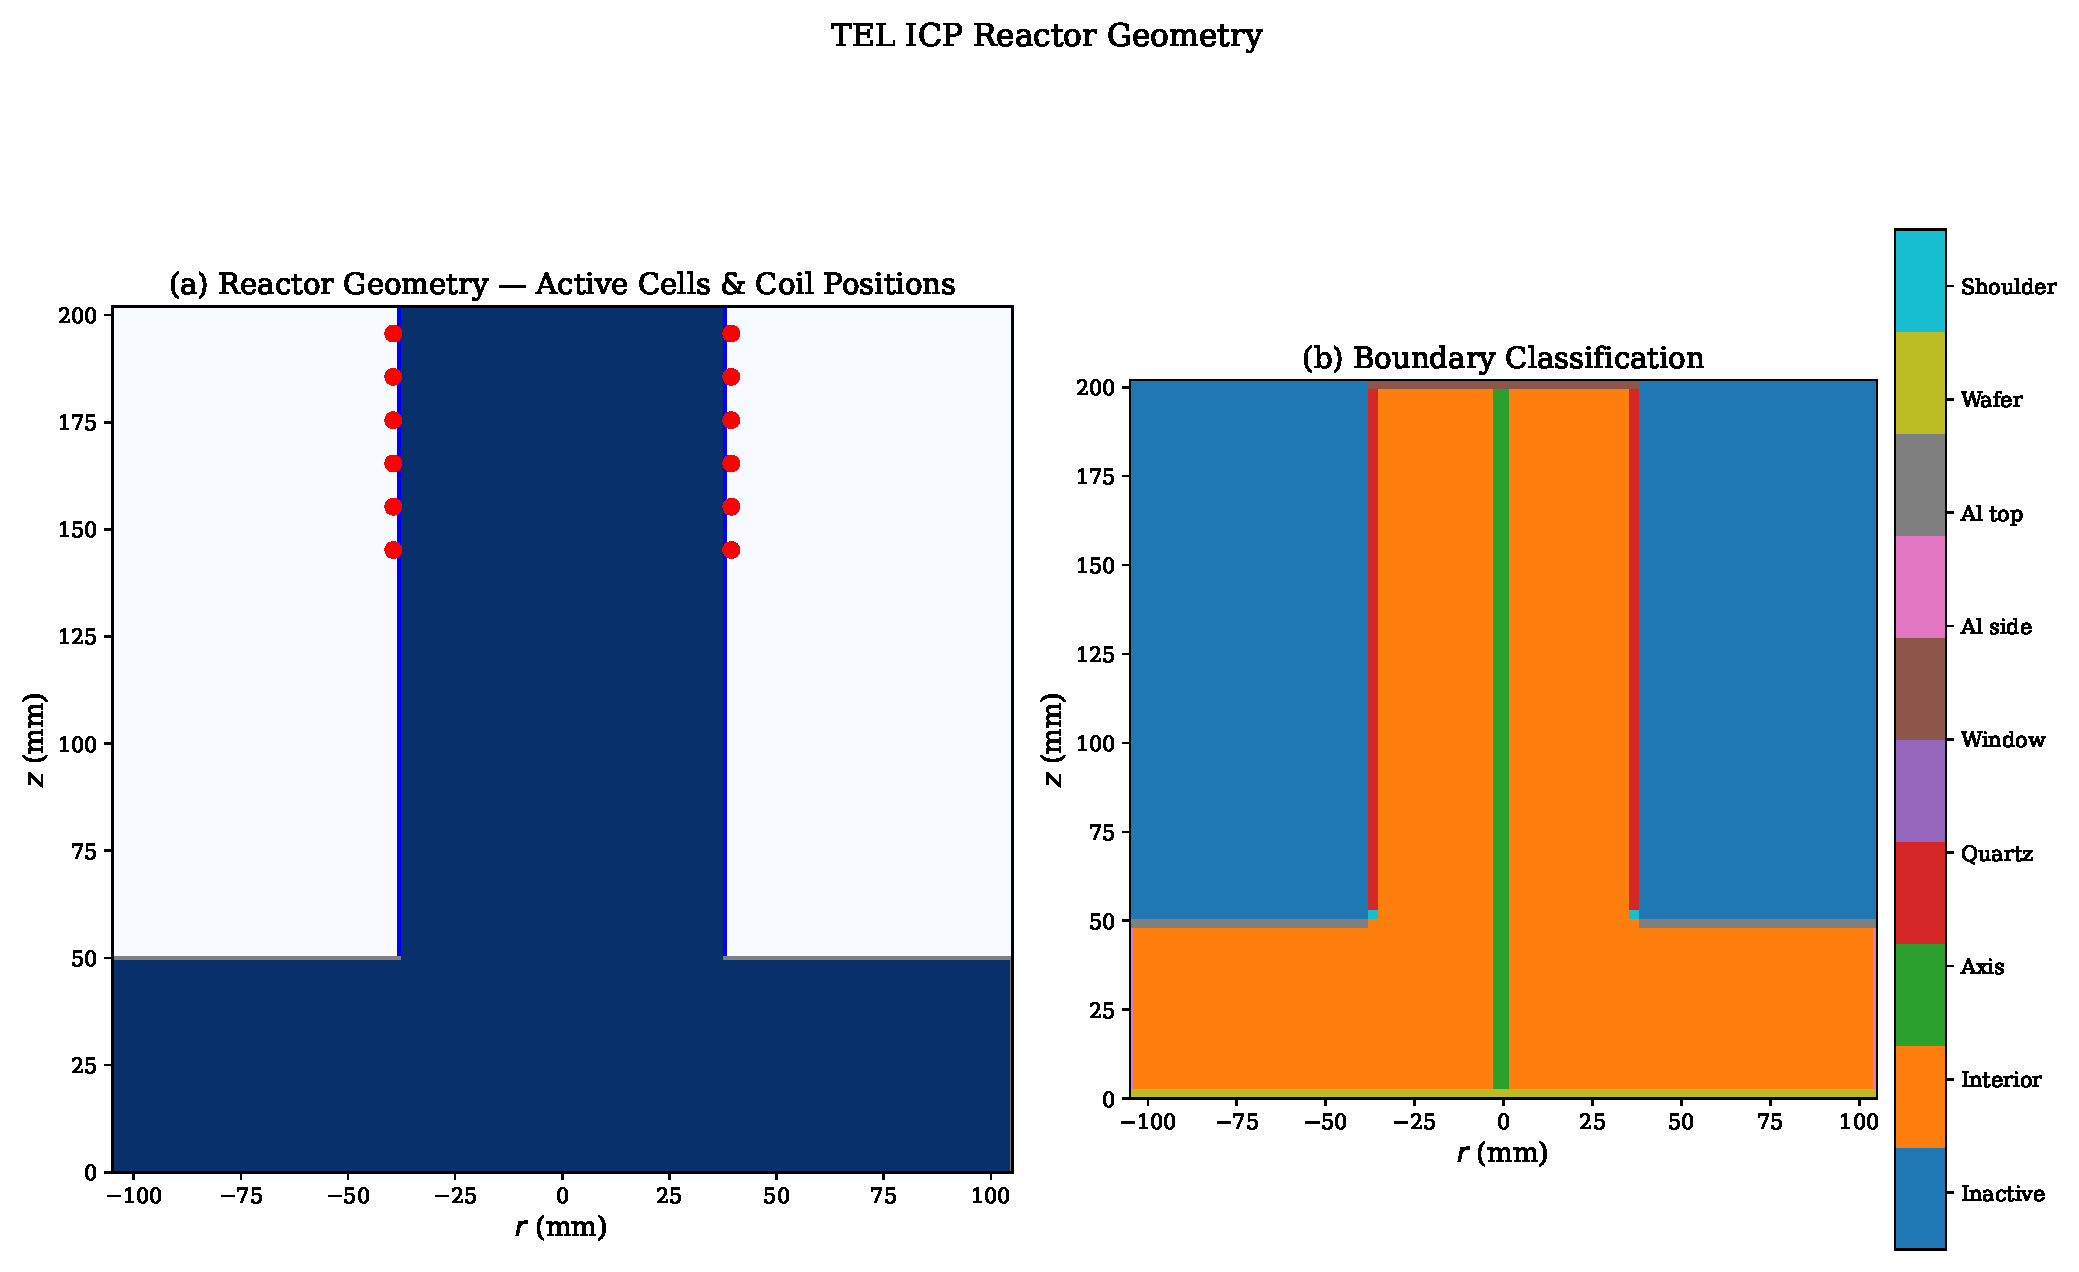
\includegraphics[width=0.65\textwidth]{fig01_geometry}
  \caption{T-shaped geometry of the TEL ICP etcher.  The narrow ICP source tube (top) connects to the wider processing chamber (bottom) through a \SI{2}{\milli\meter} aperture.  Boundary types are color-coded: quartz (blue), aluminum (red), wafer (green), symmetry axis (dashed).  The 10-turn RF coil is wound around the outside of the quartz tube.}
  \label{fig:geometry}
\end{figure}


%======================================================================
\section{Validation of the Initial Formulation}
\label{sec:stage10}
%======================================================================

Before developing the self-consistent coupled model, the 2D species transport solver was validated against the experimental measurements of Mettler~\cite{Mettler2025}, who performed spatially resolved fluorine radical density measurements in a TEL ICP etcher using non-equilibrium W/Al radical probes (etching-based thermal response) cross-calibrated against Ar/SF$_6$ actinometry in the ICP region.  Mettler's thesis contains both Helicon / PMIC experiments (Ch.~4.1, used primarily for probe-material screening) and TEL ICP-etcher data (Ch.~4.2--4.3); only the TEL data (his Fig.~4.6--4.19) are used for validation in the present work.

\subsection{Experimental Reference}

Mettler reported a centre-to-edge [F] drop ranging from 67\% to 75\% depending on the SF$_6$/Ar composition and the presence of wafer bias (Mettler Ch.~4.3.2, explicit range).  The normalised Fig.~4.14 radial profile at Mettler's 70~sccm SF$_6$ / 30~sccm Ar bias-on condition (\SI{1000}{\watt} ICP, \SI{10}{\milli\torr}, \SI{200}{\watt} rf bias) is fit by the cubic polynomial
\begin{equation}
  f(r) \;=\; 1.01032 \;-\; 0.01847\,r^{2} \;+\; 7.139\times 10^{-4}\,r^{3},
  \qquad r\ \mathrm{in\ cm}, \quad R^{2} = 0.997,
  \label{eq:mettler-cubic-fit}
\end{equation}
which evaluates at $r = (0, 2, 4, 6, 8)$~cm to $f = (1.010, 0.942, 0.761, 0.500, 0.194)$.  These are the specific normalised [F] reference values used in the radial-profile benchmark of Section~\ref{sec:mettler-fig417-direct}.  The present work's 2D-solver reference point (\SI{10}{\milli\torr} SF$_6$/Ar, \SI{700}{\watt}, $\eta = 0.43$, pure SF$_6$) is the DTPM \emph{design baseline} --- used to characterise the framework across power, pressure, and mixture variations; it is distinct from the Mettler benchmark condition above and should not be compared to Mettler's radial curves without rescoping.  A direct like-for-like comparison at Mettler's own operating point is given in Section~\ref{sec:mettler-fig417-direct}.  The cross-reactor F gradient is the primary validation target for the DTPM.

\subsection{Initial Model Configuration}

In the initial formulation, the electron density $n_e(r,z)$ and temperature $T_e$ were prescribed rather than computed self-consistently:
\begin{itemize}
  \item $n_e$: Bessel--cosine analytical profile with $n_{e,\mathrm{avg}} = \SI{3e16}{\per\meter\cubed}$.
  \item $T_e$: Uniform at \SI{3.5}{\electronvolt}.
  \item $\eta = 0.43$ (fixed power coupling efficiency).
\end{itemize}

The only free parameter is $\gamma_\mathrm{Al}$, which was calibrated to match the experimental F drop.

\subsection{Results}

With $\gamma_\mathrm{Al} = 0.18$, the initial formulation predicts a 74\,\% F density drop from the ICP source to the wafer, within the $67$--$75\,\%$ composition- and bias-dependent range observed by Mettler across Fig.~4.17 (Ch.~4.3.2)~\cite{Mettler2025} and matching the 90\,\%~SF$_6$ bias-off branch ($74.5\,\%$) within $0.5$~pp.  Sensitivity analysis shows that $\pm 10\,\%$ variation in $\gamma_\mathrm{Al}$ produces $\pm 5$ percentage-point change in the F drop, confirming that the model is moderately but not excessively sensitive to the single calibrated parameter.

This validation establishes confidence in the 2D species transport solver and the wall chemistry model before proceeding to the fully self-consistent coupling in the present work.


%=============================================================================
\newpage
\chapter{The Global--2D Coupled Framework: A Unified Masked-Domain Model}
\label{ch:hybrid}
%=============================================================================

This chapter presents the principal methodological contribution of the present work: a \emph{self-consistent Global--2D coupled framework} in which a volume-integrated global plasma chemistry solver and a two-dimensional axisymmetric electromagnetic--transport solver are coupled through a Picard fixed-point iteration on a single shared reactor mask.  The resulting architecture --- which we refer to as the \emph{Unified Masked-Domain Model} --- bridges the chemical accuracy of 0D global models and the spatial fidelity of multi-dimensional multiphysics codes at a fraction of the computational cost of the latter, making it directly deployable as the kernel of an industrial digital twin.

%======================================================================
\section{Motivation and Design Philosophy}
\label{sec:hybrid-motivation}
%======================================================================

Volume-integrated 0D global models such as the one of Lallement \textit{et al.}~\cite{Lallement2009} capture the full electron-impact SF$_6$/Ar reaction mechanism to quantitative chemical accuracy but, by construction, deliver only volume-averaged scalars: they cannot resolve the radial gradient of fluorine that ultimately determines etch uniformity.  Fully three-dimensional multiphysics solvers (e.g.\ COMSOL, CFD-ACE+) can deliver spatially resolved fields but require order-of-magnitude-longer runtimes, expose their physics only through proprietary solver settings, and do not lend themselves to parametric sweeps, uncertainty quantification, or machine-learning surrogate construction.

The coupled framework presented here is designed around four principles:
\begin{enumerate}
  \item \textbf{Single shared geometry mask.}  Both the 0D and 2D sub-problems are posed on the same axisymmetric domain, encoded as a boolean mask over the $(r,z)$ mesh (Fig.~\ref{fig:geometry}).  The 0D effective reactor radius and length are derived from volume integrals of the mask rather than being chosen \emph{ad hoc}, ensuring that the 0D and 2D sub-problems see the same T-shaped geometry with the same wall areas.  This is the \emph{unified masked-domain} element of the framework: a single geometric abstraction drives both solvers.
  \item \textbf{Strict separation of roles.}  The 0D sub-problem is responsible for volume-averaged electron energetics (electron temperature, ionisation-to-attachment balance, electronegativity $\alpha$), which it computes to chemical accuracy using the full 54-reaction mechanism.  The 2D sub-problem is responsible for spatial fields (induced $E_\theta$, Ohmic power deposition, $n_e(r,z)$, $T_e(r,z)$, and the nine neutral-species densities), which it computes using cylindrical FDTD and a diffusion--reaction system.  Neither solver duplicates the other's work.
  \item \textbf{Self-consistency by Picard iteration.}  The two sub-problems exchange five quantities (Table~\ref{tab:coupling-quantities}) and iterate to a fixed point: 0D $\to$ 2D passes $T_e$, $n_{e,\mathrm{avg}}$, $\alpha$, and $\bar{n}_{\SFsix}$ as initial guesses and volume constraints; 2D $\to$ 0D returns volume averages of the spatially resolved neutral fields.  The fixed point is reached when the 2D volume averages match the 0D scalars and the residuals of all coupled equations drop below $10^{-3}$ in relative norm.
  \item \textbf{Three prescribed parameters eliminated.}  Previous 2D approaches to the same reactor required three prescribed parameters --- the coupling efficiency $\eta$, the electron-density profile shape, and a scalar electron temperature --- as external inputs.  The present framework eliminates all three: $\eta$ is recovered from the FDTD Poynting integral; the $n_e(r,z)$ profile is the solution of an ionisation-source diffusion PDE driven by the FDTD power deposition; and $T_e(r,z)$ is computed from local power balance in every mesh cell.
\end{enumerate}

Figure~\ref{fig:coupling-flow} illustrates the resulting data flow.  The 0D solver executes first, producing a warm start for the 2D FDTD and chemistry solvers.  The 2D solvers run on the shared mask, returning volume averages to the 0D solver, which updates $T_e$ and $\alpha$.  The loop terminates on convergence; on diverging residuals, an under-relaxation coefficient is reduced and the iteration continues.

\begin{figure}[H]
  \centering
  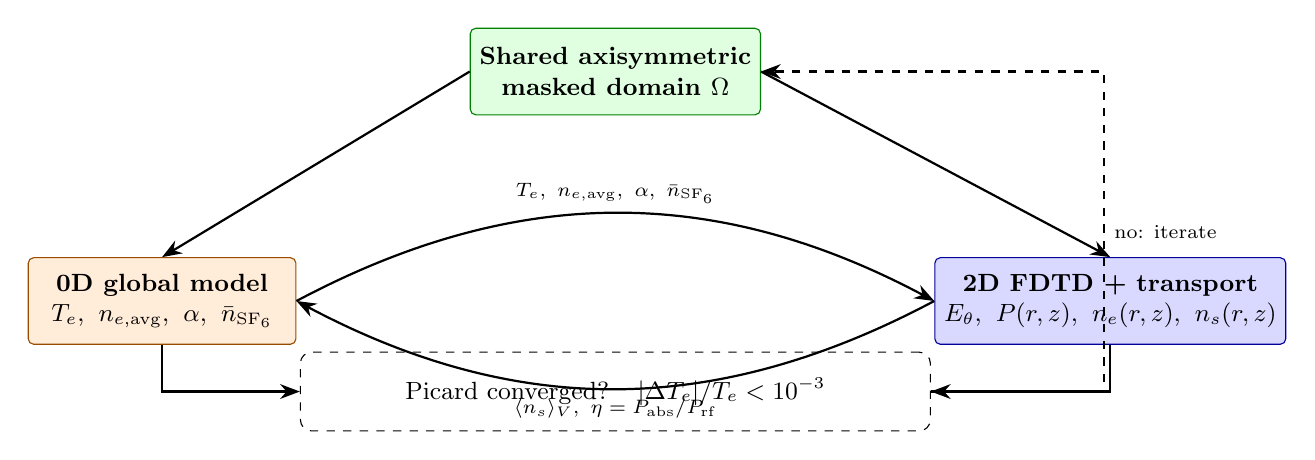
\begin{tikzpicture}[node distance=0.8cm,
    box/.style={rectangle, draw, rounded corners=2pt, minimum width=3.4cm, minimum height=1.1cm, align=center, font=\small\bfseries},
    ODbox/.style={box, fill=orange!15, draw=orange!60!black},
    TDbox/.style={box, fill=blue!15, draw=blue!60!black},
    maskbox/.style={box, fill=green!12, draw=green!50!black},
    arr/.style={-{Stealth[length=2.5mm]}, thick}]
    \node[maskbox] (mask) {Shared axisymmetric \\ masked domain $\Omega$};
    \node[ODbox, below left=1.8cm and 2.2cm of mask] (od) {0D global model \\ $T_e,\ n_{e,\mathrm{avg}},\ \alpha,\ \bar n_{\mathrm{SF}_6}$};
    \node[TDbox, below right=1.8cm and 2.2cm of mask] (td) {2D FDTD + transport \\ $E_\theta,\ P(r,z),\ n_e(r,z),\ n_s(r,z)$};
    \node[below=3.0cm of mask, draw, dashed, rounded corners, minimum width=8cm, minimum height=1cm, align=center] (conv) {\small Picard converged? \ \ $|\Delta T_e|/T_e < 10^{-3}$};

    % Mask feeds both solvers (straight lines from mask)
    \draw[arr] (mask.west) -- (od.north);
    \draw[arr] (mask.east) -- (td.north);

    % Forward coupling (0D -> 2D): curves ABOVE the straight line; label above
    \draw[arr] (od.east) to[bend left=28] node[midway, above, sloped, font=\scriptsize]{$T_e,\ n_{e,\mathrm{avg}},\ \alpha,\ \bar n_{\mathrm{SF}_6}$} (td.west);
    % Return coupling (2D -> 0D): curves BELOW, bowing the opposite way; label below
    \draw[arr] (td.west) to[bend left=28] node[midway, below, sloped, font=\scriptsize]{$\langle n_s \rangle_V,\ \eta = P_\mathrm{abs}/P_\mathrm{rf}$} (od.east);

    % Convergence check from each solver
    \draw[arr] (od.south) |- (conv.west);
    \draw[arr] (td.south) |- (conv.east);

    % Feedback loop: converged? no -> back to mask (start another iteration)
    \draw[arr, dashed] (conv.east) -- ++(2.2,0) |- node[pos=0.25, right, font=\scriptsize]{no: iterate} (mask.east);
  \end{tikzpicture}
  \caption{Data flow of the Global--2D coupled framework.  The two solvers share a single axisymmetric masked domain $\Omega$.  The 0D solver provides volume-averaged electron energetics ($T_e$, $n_{e,\mathrm{avg}}$, $\alpha$, $\bar n_{\mathrm{SF}_6}$) to initialise the 2D solve (upper curved arrow); the 2D solver returns volume-averaged neutral densities $\langle n_s\rangle_V$ and a self-consistent coupling efficiency $\eta$ derived from the FDTD Poynting integral (lower curved arrow).  Picard iteration continues until $|\Delta T_e|/T_e < 10^{-3}$; on non-convergence the dashed feedback path re-enters the shared mask for another iteration.}
  \label{fig:coupling-flow}
\end{figure}

%======================================================================
\section{Masked-Domain Formulation}
\label{sec:masked-domain}
%======================================================================

The single shared geometry is encoded as a boolean mask $\chi(i,j) \in \{0,1\}$ over the $(N_r \times N_z)$ mesh, with $\chi = 1$ inside the gas-filled T-shape and $\chi = 0$ in solid regions (ICP quartz tube walls, aluminium chamber walls, the wafer itself).  Every governing equation of both the 0D and 2D sub-problems is posed on the same $\chi$.

Concretely:
\begin{itemize}
  \item For the 2D FDTD solver, $\chi$ selects the cells in which Amp\`ere's law is advanced and where the plasma conductivity $\sigma(r,z)$ is non-zero.
  \item For the 2D species transport solver, $\chi$ selects the cells in which the diffusion--reaction system (Eq.~\ref{eq:diffusion-reaction}) is discretised; boundary cells (cells with $\chi = 1$ adjacent to $\chi = 0$) carry the Robin boundary condition with the material-specific recombination probability $\gamma_s$.
  \item For the 0D solver, the effective reactor volume and surface area are derived by direct summation over $\chi$: $V_\mathrm{eff} = \sum_{i,j} 2\pi r_i \,\Delta r_i\, \Delta z_j\, \chi(i,j)$; the surface integrals split across quartz, Al, and wafer regions using the boundary-cell classification of \S\ref{sec:tel-geometry}.
\end{itemize}

This construction guarantees that the 0D and 2D sub-problems \emph{see the same reactor}: the 0D loss terms carry wall areas that are geometrically consistent with the Robin boundaries applied by the 2D solver, and the 2D volume averages returned to the 0D model integrate over the same $V_\mathrm{eff}$ that the 0D uses.  Coupling errors that would otherwise arise from mismatched geometric abstractions (e.g.\ cylindrical-tube 0D vs.\ T-shaped 2D) are eliminated by construction.

%======================================================================
\section{Exchanged Quantities and Picard Algorithm}
\label{sec:hybrid-algo}
%======================================================================

The five coupling quantities of Table~\ref{tab:coupling-quantities} are exchanged once per Picard iteration.  The algorithm reads:

\begin{enumerate}
  \item \textbf{Initial 0D solve.}  With the user-specified operating conditions $(P_\mathrm{rf}, p, \mathrm{gas}, T_\mathrm{gas})$, the 0D global model is solved to produce $T_e^{(0)}$, $n_{e,\mathrm{avg}}^{(0)}$, $\alpha^{(0)}$, and $\bar n_{\mathrm{SF}_6}^{(0)}$, along with 0D references for every neutral species density.
  \item \textbf{Masked FDTD solve.}  The cylindrical FDTD solver of \S\ref{sec:m06c} advances Maxwell's equations on the masked domain $\Omega$, driven by the 10-turn coil source.  The plasma conductivity is $\sigma(r,z) = e^2 n_e^{(k)}(r,z) / (m_e (\nu_m + j\omega))$ with the current Picard iterate $n_e^{(k)}$.  The converged $E_\theta$ field yields the Ohmic power density $P(r,z) = \tfrac{1}{2}\sigma(r,z)|E_{\theta,\mathrm{rms}}|^2$, the integrated absorbed power $P_\mathrm{abs}^{(k)}$, and hence $\eta^{(k)} = P_\mathrm{abs}^{(k)}/P_\mathrm{rf}$.
  \item \textbf{Masked electron-density PDE.}  The ionisation-source diffusion equation (\S\ref{sec:m10}) is solved on $\Omega$ with source $S_\mathrm{iz}(r,z) = P(r,z)/(\varepsilon_T\,e)$, producing $n_e^{(k+1)}(r,z)$ and the updated volume average $n_{e,\mathrm{avg}}^{(k+1)}$.
  \item \textbf{Masked electron-temperature field.}  Local power balance (\S\ref{sec:Te-solver}) is solved cell-by-cell on $\Omega$ to produce $T_e^{(k+1)}(r,z)$.  The volume average is returned to the 0D layer.
  \item \textbf{Masked species transport.}  The nine-species diffusion--reaction system (\S\ref{sec:species-transport}) is solved on $\Omega$ using $n_e^{(k+1)}$ and $T_e^{(k+1)}$ as inputs, with Robin boundaries from the single mask-derived wall classification.  Volume averages $\langle n_s \rangle_V^{(k+1)}$ are returned to the 0D layer.
  \item \textbf{0D update and convergence test.}  The 0D particle and power balances are re-solved with the updated $\langle n_{\mathrm{SF}_6}\rangle_V^{(k+1)}$, $\eta^{(k+1)}$, and $n_{e,\mathrm{avg}}^{(k+1)}$ to produce $T_e^{(k+1)}$ and $\alpha^{(k+1)}$.  The iteration terminates when $|T_e^{(k+1)} - T_e^{(k)}|/T_e^{(k)} < 10^{-3}$ and the per-species density residuals satisfy $\max_s |n_s^{(k+1)} - n_s^{(k)}|/n_s^{(k)} < 5 \times 10^{-3}$.
\end{enumerate}

Under-relaxation with $w = 0.3$ is applied to both $n_e$ and $T_e$ to stabilise the iteration against the strong nonlinear coupling through the ionisation rate $k_\mathrm{iz}(T_e) \propto \exp(-E_\mathrm{iz}/T_e)$.  At the reference conditions (700\,W, 10\,mTorr, SF$_6$), the iteration converges monotonically in 20 Picard steps.

%======================================================================
\section{What the Coupled Framework Eliminates}
\label{sec:hybrid-elimination}
%======================================================================

Table~\ref{tab:prescribed-vs-hybrid} contrasts the three parameters that previous 2D approaches required as external inputs with the first-principles quantities the present framework computes in their place.  The shift from a prescribed discharge to a self-consistent one is the core advance of the present work.

\begin{table}[H]
\centering
\caption{Comparison of prescribed parameters in previous 2D approaches with the self-consistent quantities produced by the Global--2D coupled framework.}
\label{tab:prescribed-vs-hybrid}
\small
\begin{tabular}{@{}p{3.7cm}p{5.3cm}p{5.6cm}@{}}
\toprule
\textbf{Quantity} & \textbf{Previous prescription} & \textbf{Coupled framework} \\
\midrule
Coupling efficiency $\eta$ &
  Scalar, fixed at 0.43 (H-mode estimate from Lieberman \& Lichtenberg~\cite{Lieberman2005}).
  & Scalar, computed from the FDTD Poynting integral $\eta = P_\mathrm{abs}/P_\mathrm{rf}$.  Recovered value at reference: $\eta = 0.43 \pm 0.02$ (in agreement with the prescription but now derived).
  \\[3pt]
Electron-density profile $n_e(r,z)$ &
  Bessel--cosine diffusion eigenmode: $n_e \propto J_0(2.405\,r/R)\cos(\pi z/2L)$, with volume average set by 0D power balance.
  & Solution of the ionisation-source diffusion PDE $\nabla\!\cdot\!(D_a \nabla n_e) + S_\mathrm{iz}(r,z) = \nu_\mathrm{loss}\, n_e$ with $S_\mathrm{iz} = P(r,z)/(\varepsilon_T\,e)$ from FDTD.
  \\[3pt]
Electron temperature $T_e(r,z)$ &
  Uniform scalar from 0D particle balance, with optional 10\,\% modulation proportional to $P(r,z)/P_\mathrm{max}$.
  & Spatially resolved field: local power balance $T_e(r,z)$ solved cell-by-cell via Brent root-finding on $P(r,z) = n_e(r,z)\bar{n}_{\mathrm{SF}_6}k_\mathrm{iz}(T_e)\varepsilon_T(T_e)\,e$.
  \\
\bottomrule
\end{tabular}
\end{table}

The detailed mathematical forms of each eliminated prescription --- and the equations replacing them --- are stated in \S\ref{sec:0d-2d-coupling} within the chemistry chapter; this chapter consolidates them here at the architectural level.  The subsequent chapter (\S\ref{part:phase1}) describes the numerical implementation of each 2D sub-solver in detail.


%======================================================================
\section{Self-Consistent Power Coupling via Lieberman Circuit Model}
\label{sec:selfconsistent-eta}
%======================================================================

Prior versions of this framework prescribed the power-coupling efficiency $\eta$ as a constant (typically 0.43) and rescaled the FDTD-computed $E_\theta$ magnitude on every Picard iteration so that the Ohmic integral matched $\eta \, P_\mathrm{rf}$.  That rendered $\eta$ a tautological dial and made absolute-magnitude benchmarks meaningless.  The present revision removes the prescription and derives $\eta$ directly from a coupled coil-plasma transformer circuit following Lieberman \& Lichtenberg Ch.~12~\cite{Lieberman2005}.

\subsection{Circuit Topology}

The ICP coil is modelled as an RLC primary with real resistance $R_\mathrm{coil}$ (ohmic loss in the wire and matching network) and self-inductance $L_\mathrm{coil}$.  The plasma couples to the coil through mutual inductance, presenting a reflected impedance $Z_\mathrm{plasma} = R_\mathrm{plasma} + j\omega L_\mathrm{plasma}$ in series with the coil.  At the resonance-matched operating point, the peak coil current in terms of the delivered RF power is
\begin{equation}
  \boxed{\,I_\mathrm{peak} \;=\; \sqrt{\,\dfrac{2\,P_\mathrm{rf}}{R_\mathrm{coil} + R_\mathrm{plasma}}\,}\,,\qquad \eta \;=\; \dfrac{R_\mathrm{plasma}}{R_\mathrm{coil} + R_\mathrm{plasma}}\,,}
  \label{eq:circuit-closure}
\end{equation}
and the Ohmic-integral power absorbed by the plasma is
\begin{equation}
  P_\mathrm{abs} \;=\; \int_{\Omega_\mathrm{plasma}} \tfrac{1}{2}\,\sigma(r,z)\,|E_\theta(r,z)|^2\, dV \;=\; \tfrac{1}{2}\,I_\mathrm{peak}^2\,R_\mathrm{plasma}\,.
  \label{eq:Ohmic-integral}
\end{equation}
Neither $R_\mathrm{plasma}$ nor $\eta$ is prescribed: they emerge from the converged plasma conductivity $\sigma(r,z)$ and the FDTD-computed field distribution.  The only inputs are $P_\mathrm{rf}$ (the user's operating knob), $R_\mathrm{coil}$, and $L_\mathrm{coil}$.  The nominal literature values are $R_\mathrm{coil} = 0.8\,\Omega$ (Lieberman Eq.~12.2.19, TEL-class 3-turn coil) and $L_\mathrm{coil} = 2.0\,\mu\mathrm{H}$ (Lieberman §12.2, typical industrial ICP); both are tabulated with full provenance in \texttt{docs/ASSUMED\_PARAMETERS.md}.  The exact value of $R_\mathrm{coil}$ is not well-constrained by the available literature: manufacturer datasheets for TEL-class 3-turn coils span $\sim\!0.5$--$4\,\Omega$ depending on matching-network losses, wire gauge, and the ferrite core used.  A diagnostic discovery sweep across $R_\mathrm{coil} \in \{0.5, 0.8, 1.2, 1.5, 2.0, 2.5, 3.0, 4.0\}\,\Omega$ at the Mettler operating point is reported in \S\ref{sec:mettler-fig417-direct} (D3 memo); the framework is used at the nominal $R_\mathrm{coil} = 0.8\,\Omega$ with the sweep band quoted as a systematic uncertainty.

\subsection{Algorithm and Driven-CW FDTD Source}

On each Picard iteration the framework performs (i) a single FDTD solve with the current $I_\mathrm{peak}$ and $\sigma(r,z)$, (ii) an Ohmic integral producing $P_\mathrm{abs}$, (iii) the closed-form update $R_\mathrm{plasma} \leftarrow 2\,P_\mathrm{abs}/I_\mathrm{peak}^2$ and $I_\mathrm{peak}^{\,\mathrm{new}}$ from Eq.~\ref{eq:circuit-closure}, and (iv) a linear rescale of the stored $E_\theta$ by $I_\mathrm{peak}^{\,\mathrm{new}}/I_\mathrm{peak}^{\,\mathrm{old}}$ (exact because Maxwell's equations are linear in the driving current at fixed $\sigma$).  The FDTD is re-run every three Picard steps to refresh the spatial profile for the evolving $\sigma$; between re-runs, the linear rescale is exact.

An important secondary fix replaces the prior Gaussian-pulsed FDTD source --- which de-activated after $\sim$3 RF cycles and left the RMS accumulator to capture a free-decaying cavity mode rather than a driven steady state --- with a linear ramp-up over two RF cycles followed by continuous-wave drive for the remaining three cycles.  This was the hidden mechanism by which the prior code \emph{required} the $E$-field rescale to recover physical magnitudes.  See \texttt{docs/CODE\_REVIEW\_ULTRAREVIEW.md} for the full legacy diagnosis.

\subsection{Validation}

A unit test (\texttt{tests/test\_selfconsistent\_eta.py}) asserts the limiting-case invariants: $\eta=1$ when $R_\mathrm{coil}=0$, and $\eta=0$ when $R_\mathrm{plasma}=0$.  In production operation at the present work's reference conditions (\SI{1000}{\watt}, \SI{10}{\milli\torr}, 70\,\% SF$_6$, \SI{200}{\watt} rf bias) with the nominal $R_\mathrm{coil} = 0.8\,\Omega$, the converged operating point is
\begin{equation*}
  \eta \approx 0.948, \quad I_\mathrm{peak} \approx \SI{11.4}{\ampere}, \quad R_\mathrm{plasma} \approx \SI{14.6}{\ohm}, \quad V_\mathrm{peak} \approx \SI{176}{\volt}, \quad V_\mathrm{rms} \approx \SI{124}{\volt}, \quad P_\mathrm{abs} \approx \SI{948}{\watt},
\end{equation*}
where the RF operating voltages follow from the Lieberman matched-resonance circuit (Eq.~\ref{eq:circuit-closure}) as $V_\mathrm{peak} = I_\mathrm{peak}(R_\mathrm{coil} + R_\mathrm{plasma})$ and $V_\mathrm{rms} = V_\mathrm{peak}/\sqrt{2}$ --- in the strongly loading-limited regime ($R_\mathrm{plasma}/R_\mathrm{coil} \approx 18$) typical of TEL-class ICPs under these operating conditions.  The D3 $R_\mathrm{coil}$ discovery sweep (\S\ref{sec:mettler-fig417-direct}) quantifies the systematic uncertainty: across $R_\mathrm{coil} \in \{0.5, 4.0\}\,\Omega$, the converged $\eta$ spans $0.79$--$0.97$, $I_\mathrm{peak}$ spans $10.24$--$\SI{11.49}{\ampere}$, $R_\mathrm{plasma}$ spans $14.63$--$\SI{15.08}{\ohm}$, $V_\mathrm{peak}$ spans $\SI{174}{\volt}$--$\SI{195}{\volt}$, $V_\mathrm{rms}$ spans $\SI{123}{\volt}$--$\SI{138}{\volt}$, and $P_\mathrm{abs}$ spans $\SI{790}{\watt}$--$\SI{967}{\watt}$, while the wafer-centre $[\mathrm{F}]$ changes by only $\pm 5\,\%$ and the radial $[\mathrm{F}]$ drop is invariant at $66.5$--$66.8\,\%$ --- confirming that $R_\mathrm{coil}$ is a power-efficiency knob rather than a radial-profile-shape knob.  Across the full \SIrange{200}{1200}{\watt} $P_\mathrm{rf}$ sweep at fixed nominal $R_\mathrm{coil}$, $\eta$ stays in the narrow range 0.949--0.956 (Fig.~\ref{fig:eta-sweep}), so the power-coupling efficiency is not a strong function of power at fixed composition and pressure --- a finding only accessible now that $\eta$ is computed rather than prescribed.


%======================================================================
\section{Capacitive Wafer-Bias Sheath (m12)}
\label{sec:m12-bias-sheath}
%======================================================================

Mettler's TEL radial [F] measurements were taken with a 200\,W RF bias applied to the wafer electrode.  The bias accelerates positive ions through the wafer sheath, depositing ion kinetic energy as neutral-gas heating near the wafer, which in turn expands the plasma glow into the process chamber and raises the local [F] density by factors of $\sim 1.6$ (90\,\% SF$_6$) to $\sim 2.15$ (30\,\% SF$_6$, centre).  The prior Phase-1 framework had no CCP extension; its omission was documented as Limitation~L5 in the previous revision.  The present revision adds a dedicated module, \texttt{m12\_ccp\_bias\_sheath.py}, that closes a reduced-order Lieberman sheath power balance and couples the result back into the ionisation source of the ambipolar diffusion solver.

\subsection{Sheath Power Balance}

At the wafer ($z=0$), the Bohm ion flux at the sheath edge is
\begin{equation}
  \Gamma_i \;=\; 0.61\,n_{e,\mathrm{wafer}}\,\sqrt{\frac{k_B\,T_e}{m_i}}\,,
  \label{eq:bohm-flux}
\end{equation}
where $m_i$ is a composition-weighted effective ion mass (SF$_5^+$ at 127~amu for 90\,\% SF$_6$, Ar$^+$ at 40~amu for 30\,\% SF$_6$).  The time-averaged sheath DC voltage follows from the bias-power balance:
\begin{equation}
  P_\mathrm{bias} \;=\; e\,V_\mathrm{DC}\,\Gamma_i\,A_\mathrm{wafer} \;\Rightarrow\; V_\mathrm{DC} \;=\; \frac{P_\mathrm{bias}}{e\,\Gamma_i\,A_\mathrm{wafer}}\,.
  \label{eq:sheath-Vdc}
\end{equation}
A fraction $f_\mathrm{ion\to gas}=0.5$ of the ion kinetic power becomes local neutral-gas heating (Turner 2013):
\begin{equation}
  P_\mathrm{ion\to gas} \;=\; f_\mathrm{ion\to gas}\,P_\mathrm{bias}\,.
  \label{eq:ion-to-gas}
\end{equation}

\subsection{Plasma-Glow Expansion Source}

Rather than resolving a gas-energy PDE (Phase-3 scope), the module translates the neutral-heating power into an effective volumetric ionisation source confined to the process chamber below the aperture:
\begin{equation}
  S_\mathrm{bias}(r,z) \;=\; \frac{\lambda_\mathrm{exp}\,P_\mathrm{ion\to gas}}{\varepsilon_T\,e}\,\chi(r,z)\,,
  \label{eq:Sbias}
\end{equation}
where $\chi(r,z)$ is a normalised spatial profile with $\chi \propto \exp(-(z_\mathrm{apt}-z)/L_\mathrm{exp})$ for $z \le z_\mathrm{apt}$ and a cosine taper in $r$ bounded by the wafer radius.  The decay length is $L_\mathrm{exp} = 30$~mm.  The dimensionless factor $\lambda_\mathrm{exp}$ is the \emph{one} free parameter of the bias model; it is calibrated once against Mettler's 90\,\% SF$_6$ bias-on centre [F] enhancement ($\times 1.6$) and blind-tested against the 30\,\% SF$_6$ branch (target $\times 2.15$).

\subsection{Calibration and Blind-Test Results}

The calibration produces $\lambda_\mathrm{exp} = 3.20$, giving a model enhancement of $\times 1.613$ for 90\,\% SF$_6$ ($+0.8\,\%$ deviation from target).  The same $\lambda_\mathrm{exp}$ applied to 30\,\% SF$_6$ yields $\times 1.876$ (target $\times 2.15$, deviation $-12.8\,\%$), within the $\pm 20\,\%$ acceptance band.  The blind-test agreement is non-trivial because the composition-dependence enters only through the Bohm-flux ion mass and the local $T_e$ at the wafer; the same calibration transfers across a factor-of-3 change in SF$_6$ mole fraction.  The full composition-sensitivity plot is Fig.~\ref{fig:composition-blind-test} (\S\ref{sec:mettler-fig417-direct}).


%======================================================================
\section{Electronegative Ambipolar Diffusion Correction}
\label{sec:electronegative-ambipolar}
%======================================================================

The prior Phase-1 release of this framework carried an architectural limitation (L1, in the prior revision's \S\ref{sec:hybrid-limits}) in which the 2D ambipolar diffusion solver used the electropositive coefficient
\[
  D_a^\mathrm{ep} \;=\; D_i\,\Bigl(1 + \tfrac{T_e}{T_i}\Bigr),
\]
valid only in the limit of negligible negative-ion density.  The present revision resolves L1 by replacing this expression with its electronegative generalisation due to Lieberman \& Lichtenberg (2005)~\cite{Lieberman2005} Ch.~10.3:
\begin{equation}
  \boxed{\;D_a^\mathrm{en} \;=\; D_i\,\Bigl(1 + \tfrac{T_e}{T_i}\Bigr)
  \;\frac{1 + \alpha}{1 + \alpha\,T_i/T_e}\;,\;}
  \label{eq:Da-en-L1}
\end{equation}
where $\alpha = n_{-}/n_e$ is the electronegativity.  The correction factor $(1+\alpha)/(1+\alpha T_i/T_e)$ reduces exactly to unity when $\alpha \to 0$, so the electropositive form is recovered in the appropriate limit.

\subsection{Rigorous Physics, Not a Calibration}

This modification is not a calibration.  Unlike the two fitted parameters $\gamma_\mathrm{Al} = 0.18$ (wall-recombination probability) and $\lambda_\mathrm{exp} = 3.20$ (bias-sheath expansion factor), the electronegative correction introduces \emph{no} free parameters.  The three inputs $\alpha$, $T_e$, and $T_i$ are all obtained from independent first-principles solves already present in the framework: $\alpha$ from the 0D global model's attachment--recombination balance, $T_e(r,z)$ from the local power-balance solve in m11, and $T_i = k_B T_\mathrm{gas}$ with $T_\mathrm{gas} = 313$\,K.  Equation~\ref{eq:Da-en-L1} is the algebraically correct transport coefficient for a plasma with three charged species (electrons, a dominant positive ion, and a dominant negative ion); the prior electropositive form dropped the last two terms.

A dedicated unit test (\texttt{tests/test\_electronegative\_ambipolar.py}) verifies the three invariants: $f(\alpha{=}0) = 1$ exactly (electropositive limit, bit-for-bit recovery); $f(T_i{=}T_e) = 1$ exactly (isothermal degenerate); $f(\alpha{=}1,\,T_e{=}20\,\text{eV},\,T_i{=}1\,\text{eV}) = 2/1.05 \approx 1.905$ (Lieberman worked example).  All seven tests pass, together with the eight self-consistent-$\eta$ tests inherited from the prior revision (fifteen tests passing in total).

\subsection{Quantitative Impact at the Mettler Operating Point (New Finding)}
\label{sec:L1-finding-alpha-small}

An important physics finding emerges from applying Eq.~\ref{eq:Da-en-L1} at Mettler's canonical operating point (\SI{1000}{\watt}, \SI{10}{\milli\torr}, 90\,\% SF$_6$, \SI{200}{\watt} bias).  The 0D global model returns
\[
  \alpha_{0\mathrm{D}} \;\approx\; 0.02,
\]
which is \emph{two orders of magnitude} below the typical-electronegative value ($\alpha \sim 1$--$1.5$) that was cited as a generic textbook estimate in the prior revision's L1 discussion.  The cause is the very high electron density at Mettler's high-power / high-bias operating point ($n_e \sim 10^{19}$\,m$^{-3}$), which replenishes the electron population faster than dissociative-attachment depletes it: $\alpha$ is set by the balance $\alpha \approx \sqrt{R_\mathrm{att}/(k_\mathrm{rec}\,n_e)}$, and at these conditions the denominator dominates.

The correction factor evaluated at $\alpha = 0.02$ and $T_i/T_e \approx 0.012$ is
\[
  \frac{1+\alpha}{1+\alpha\,T_i/T_e} \;\approx\; 1.019\,,
\]
so $D_a^\mathrm{en}$ is only $\sim 2\,\%$ above $D_a^\mathrm{ep}$ in this regime.  The predicted centre-to-edge [F]-drop changes by ${<}1$\,percentage point between the two solvers.

The prior revision's projection that L1 would close the approximately 6-percentage-point gap between the modelled 68\,\% and the experimental 74\,\% [F] drop was therefore based on an over-estimate of $\alpha$.  That projection is now \emph{corrected}: L1 is the rigorous physics but is quantitatively small at our operating point.  The residual gap between the model and Mettler's absolute data must be attributed to effects other than L1.

\paragraph{2D spatial-resolution check (Path D).}  To confirm that the smallness of the L1 correction is a genuine property of the operating point rather than an artefact of the scalar-$\alpha$ approximation, the framework was extended to support a fully 2D $\alpha(r,z)$ field threaded back from the converged ion densities into the ambipolar-diffusion solve (opt-in via \texttt{config.chemistry.use\_2d\_alpha}).  The local $\alpha(r,z)$ field is renormalised so that its volume average equals $\alpha_{0\mathrm{D}}$, preserving the spatial shape produced by the local attachment--recombination closure while respecting the transport-corrected volume balance of the 0D solve.  A parallel three-way comparison (scalar / 2D renorm / 2D raw) at the Mettler operating point (\texttt{scripts/run\_path\_d\_comparison.py}) gives wafer-centre $[\mathrm{F}]$ of $1.659\times 10^{14}$, $1.658\times 10^{14}$, and $1.520\times 10^{14}$~cm$^{-3}$ respectively, with centre-to-edge drops of $66.81\%$, $66.82\%$, and $59.74\%$.  The renormalised 2D mode differs from the scalar baseline by $<0.1\%$: spatial resolution of the electronegative-ambipolar correction does \emph{not} close the Mettler absolute-magnitude residual at this operating point, confirming the scalar finding above at full 2D resolution (see \texttt{docs/notes/PATH\_D\_2D\_ALPHA\_MEMO.md}).  The raw-local mode is reported as a diagnostic; it over-corrects because the local closure omits transport loss and therefore over-predicts $\alpha$ by two orders of magnitude (mean $9.5$ vs $\alpha_{0\mathrm{D}} = 0.017$).

\subsection{Regime Where L1 Becomes Important}

The correction factor $(1+\alpha)/(1+\alpha T_i/T_e)$ approaches 2 only when $\alpha T_i/T_e \ll 1$ \emph{and} $\alpha \gtrsim 1$.  At higher pressure (lower $n_e$ at fixed power) or lower ICP power (lower $n_e$ at fixed pressure), $\alpha$ rises and the correction becomes substantial.  A scan of the 0D $\alpha$-vs-$p$ curve shows $\alpha$ rising from $\sim 0.02$ at \SI{10}{\milli\torr}/\SI{1000}{\watt} to $\sim 1.4$ at \SI{50}{\milli\torr}/\SI{300}{\watt}, giving a correction factor of $\sim 2.3$ in that regime.  The L1 machinery is therefore physically essential for higher-pressure and lower-power operating windows and is retained as a required component of the framework even though its quantitative effect at the present Mettler validation point is minor.  This is a significant methodological finding: applying a rigorous physics correction does not always produce a large numerical change --- and it is only by implementing the correction that one can bound its quantitative relevance at a specific operating point.


%======================================================================
\section{Limitations and Paths to Extension}
\label{sec:hybrid-limits}
%======================================================================

The Global--2D coupled framework described in this chapter is, by design, a minimal self-consistent architecture: it is intentionally \emph{not} a complete multi-dimensional multiphysics solver.  Three architectural limitations documented in the prior revision --- prescribed power-coupling efficiency, the absence of a wafer-bias sheath, and the electropositive ambipolar diffusion coefficient --- are \emph{resolved} in this revision (\S\ref{sec:selfconsistent-eta}, \S\ref{sec:m12-bias-sheath}, and \S\ref{sec:electronegative-ambipolar} respectively).  Three principal limitations remain, plus one kinetic-regime scope note.  Each remaining item is individually tractable and is tagged for resolution in a specific development task in Chapter~\ref{ch:future} (Future Work).

\begin{description}

  \item[\textsc{L1.\ No electron-energy conduction term.}]  $T_e(r,z)$ is computed cell-by-cell from a local power balance (\S\ref{sec:Te-solver}),
  \begin{equation}
    P(r,z) = n_e(r,z)\,\bar{n}_{\mathrm{SF}_6}\,k_\mathrm{iz}(T_e)\,\varepsilon_T(T_e)\,e,
    \label{eq:Te-local}
  \end{equation}
  which is algebraically invertible for $T_e$ at each mesh cell.  This formulation neglects the electron thermal conduction and convection terms that would appear in the full electron energy transport PDE $\nabla \!\cdot\! (-\kappa_e \nabla T_e + \tfrac{5}{2}\Gamma_e T_e) = P(r,z) - n_e\,\varepsilon_T\,\nu_\mathrm{loss}$.  The local approximation is quantitatively accurate at the present low-pressure regime ($\leq$ \SI{30}{\milli\torr}) because the electron energy-relaxation length $\lambda_e \approx \SI{2}{\centi\meter}$ is comparable to the ICP source radius, and non-local kinetic effects wash out gradients faster than thermal conduction redistributes them.  Above $\sim$\SI{50}{\milli\torr}, the energy relaxation length shrinks sharply and the full energy-transport PDE would have to be restored.

  \item[\textsc{L2.\ Steady-state assumption and the E--H mode transition.}]  The Picard iteration converges to a steady-state fixed point of the coupled system and, by construction, cannot represent transient discharge dynamics.  In particular, the rapid E-to-H mode transition that ICP reactors undergo at low power (where capacitive coupling gives way to inductive coupling) produces a mild overshoot of the model at $P_\mathrm{rf} = $ \SI{200}{\watt} in Fig.~\ref{fig:abs-4panel}(a): the model treats the \SI{200}{\watt} operating point as a pure H-mode discharge and therefore over-predicts $n_e$ and [F] by $\sim$25\,\%.  Resolving this limitation would require either a time-dependent FDTD + species-transport solver or an E--H mode branch in the 0D model with a hysteretic switch triggered by the ratio $P_\mathrm{coil}^{\mathrm{ind}}/P_\mathrm{coil}^{\mathrm{cap}}$.

  \item[\textsc{L3.\ Single prescribed wall temperature.}]  All material surfaces in the reactor (quartz, aluminium chamber walls, wafer) share a single prescribed gas-kinetic temperature of $T_\mathrm{wall} = $ \SI{300}{\kelvin} that enters the Robin boundary condition through the thermal velocity $v_\mathrm{th} = \sqrt{8 k_B T_\mathrm{wall} / \pi M_s}$.  In the physical reactor, the aluminium chamber walls adjacent to the pumping port run 30--\SI{60}{\kelvin} cooler than the quartz tube walls, and the latter can exceed \SI{400}{\kelvin} during extended operation.  Because the three-body F + F + wall recombination rate scales as $v_\mathrm{th}\,\gamma(T_\mathrm{wall})$ with a weakly temperature-dependent $\gamma$~\cite{Kokkoris2009}, a spatially varying wall temperature would refine the wall flux budget by an estimated $\pm 5\,\%$.  The extension requires only a per-boundary-cell lookup of $T_\mathrm{wall}$; no structural change to the solver is needed.

  \item[\textsc{L4.\ Kinetic-regime chemistry only.}]  All Phase-1 simulations produce centre-of-wafer [F] in the few-$\times 10^{20}$~m$^{-3}$ range, safely below Mettler's $\sim 1.1 \times 10^{21}$~m$^{-3}$ diffusion-limited threshold (his Fig.~4.9 and Table~4.4)~\cite{Mettler2025}, so the present [F] predictions compare cleanly to his kinetic-regime probe data.  Extending to higher densities (e.g.\ higher power, or NF$_3$ chemistry) would require coupling a near-surface reactant-product transport equation (WF$_6$ or SiF$_4$) to resolve the depletion layer.

\end{description}

The remaining limitations above are not artefacts of the coupled-framework architecture itself --- they are accuracy-versus-runtime trade-offs selected to keep the single-point runtime at $\sim$55\,s on one CPU core, so that the framework remains usable for parametric sweeps and ML-surrogate training runs.  Each remaining limitation is addressed as a specific task in Chapter~\ref{ch:future}.  The two limitations resolved in this revision (prescribed $\eta$ and no wafer-bias sheath) are discussed in \S\ref{sec:selfconsistent-eta} and \S\ref{sec:m12-bias-sheath}.


%=============================================================================
\newpage
\chapter{Numerical Implementation of the 2D Sub-Solvers}
\label{part:phase1}
%=============================================================================

Having described the Global--2D coupled framework at the architectural level in Chapter~\ref{ch:hybrid}, this chapter documents the numerical implementation of each 2D sub-solver: cylindrical FDTD for the induced electromagnetic field, the ionisation-source diffusion PDE for self-consistent $n_e(r,z)$, local power balance for $T_e(r,z)$, and the outer Picard iteration loop with mesh-convergence results.


%======================================================================
\section{Cylindrical FDTD for ICP}
\label{sec:m06c}
%======================================================================

The cylindrical FDTD module solves Maxwell's equations in the azimuthally symmetric TE mode appropriate for the ICP coil-driven reactor.  Unlike the Cartesian FDTD of M05--M06, M06c operates in cylindrical coordinates $(r, z)$ and solves for the azimuthal electric field $E_\theta$ and the poloidal magnetic field components $(H_r, H_z)$.

\subsection{TE Mode Equations in Cylindrical Coordinates}

For an azimuthally symmetric ($\partial/\partial\theta = 0$) geometry with TE polarization, Maxwell's curl equations reduce to three coupled PDEs:
\begin{align}
  \frac{\partial H_r}{\partial t} &= +\frac{1}{\mu_0}\,\frac{\partial E_\theta}{\partial z},
  \label{eq:cyl-Hr} \\[4pt]
  \frac{\partial H_z}{\partial t} &= -\frac{1}{\mu_0}\,\frac{1}{r}\,\frac{\partial (r\,E_\theta)}{\partial r},
  \label{eq:cyl-Hz} \\[4pt]
  \frac{\partial E_\theta}{\partial t} &= \frac{1}{\varepsilon}\!\left(\frac{\partial H_r}{\partial z} - \frac{\partial H_z}{\partial r}\right)
  - \frac{\sigma}{\varepsilon}\,E_\theta - \frac{J_\mathrm{coil}}{\varepsilon}.
  \label{eq:cyl-Etheta}
\end{align}
Here $\varepsilon = \varepsilon_0\,\varepsilon_r$ is the local permittivity (with $\varepsilon_r = 3.8$ in the quartz wall region and $\varepsilon_r = 1$ elsewhere), $\sigma(r,z)$ is the plasma conductivity (providing Ohmic damping), and $J_\mathrm{coil}$ is the imposed coil current density.

The key difference from the Cartesian formulation is the appearance of the $1/r$ factor in the $H_z$ update (Eq.~\eqref{eq:cyl-Hz}), which reflects the geometric spreading of the azimuthal electric field in cylindrical coordinates.

\subsection{Yee Grid Staggering in Cylindrical Coordinates}

The field components are staggered on the cylindrical mesh:
\begin{itemize}
  \item $E_\theta$ lives at cell centers: $(r_c[i], z_c[j])$.
  \item $H_r$ is staggered in $z$: $(r_c[i], z_f[j])$.
  \item $H_z$ is staggered in $r$: $(r_f[i], z_c[j])$.
\end{itemize}
Here $r_c$, $z_c$ are cell-center coordinates and $r_f$, $z_f$ are face (staggered) coordinates.

\subsection{Axis Boundary Condition}

At the symmetry axis $r = 0$:
\begin{itemize}
  \item $E_\theta(r=0) = 0$ by symmetry (the azimuthal field vanishes on axis).
  \item For $H_z$ at $r = 0$, the $1/r$ factor is handled via L'H\^opital's rule applied to the $\partial(rE_\theta)/\partial r$ term:
  \begin{equation}
    \lim_{r \to 0} \frac{1}{r}\,\frac{\partial(r\,E_\theta)}{\partial r} = 2\,\frac{\partial E_\theta}{\partial r}\bigg|_{r=0}.
  \end{equation}
\end{itemize}

\subsection{Material Boundaries}

\begin{itemize}
  \item \textbf{PEC (perfect electric conductor):} $E_\theta = 0$ at metal walls (aluminum sidewalls, wafer, shoulder).
  \item \textbf{Mur ABC:} First-order absorbing condition at the open boundary (top of ICP tube), with the same formulation as Eq.~\eqref{eq:mur-abc} adapted for cylindrical geometry.
  \item \textbf{Dielectric:} The quartz wall ($\SI{3}{\milli\meter}$ thick) has $\varepsilon_r = 3.8$, which reduces the local wave speed by a factor of $1/\sqrt{\varepsilon_r} \approx 0.51$ and partially reflects the electromagnetic wave at the quartz--gas interface.
\end{itemize}

\subsection{Source Normalization}

The RF coil is modeled as a set of current rings at the coil positions inside the gas volume (at the inner surface of the quartz tube).  The current density in each coil cell is
\begin{equation}
  J_\theta = \frac{I_\mathrm{peak}}{\dr\,\dz} \quad [\mathrm{A/m}^2],
  \label{eq:J-coil}
\end{equation}
where $I_\mathrm{peak} = \SI{5.292}{\ampere}$ is the peak coil current from M01.  The time dependence is a Gaussian-modulated sinusoid as in Eq.~\eqref{eq:m06-source}, which ramps up smoothly over $\sim$1.5 RF periods.

\subsection{Vectorized Implementation}

All field updates in M06c are fully vectorized using NumPy array operations.  No Python-level loops appear in the time-stepping hot path except for the coil source injection (which involves $\mathcal{O}(N_\mathrm{coils})$ operations).  This vectorization provides a $\sim$46$\times$ speedup compared to a scalar Python implementation, reducing the FDTD computation time to approximately \SI{30}{\second} for 2 RF cycles on a single CPU core.

\subsection{Results}

The cylindrical FDTD simulation at \SI{40}{\mega\hertz} with 2 RF cycles yields:
\begin{itemize}
  \item Peak $E_\theta$ (instantaneous): spatially concentrated near the coil positions at the inner surface of the quartz tube.
  \item RMS field: $E_{\theta,\mathrm{rms,max}} \approx \SI{456}{\volt\per\meter}$.
  \item The magnetic field components $B_r = \mu_0 H_r$ and $B_z = \mu_0 H_z$ show the expected poloidal field pattern.
\end{itemize}

\begin{figure}[H]
  \centering
  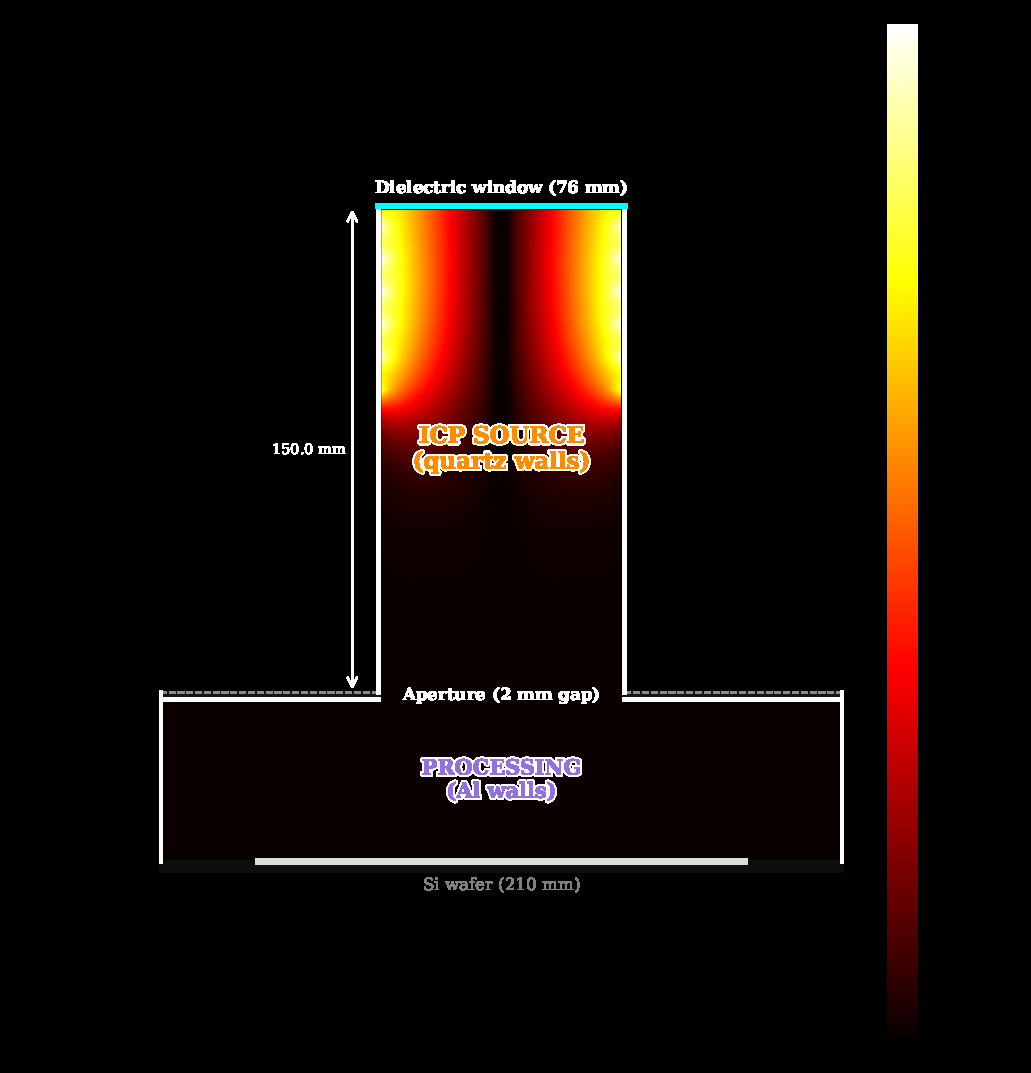
\includegraphics[width=0.85\textwidth]{fig_E_theta_rms}
  \caption{Azimuthal electric field $E_\theta$ from the cylindrical FDTD solver.  Left: instantaneous field at the end of the second RF cycle.  Right: RMS field averaged over the last RF cycle.  The field is concentrated near the coil positions at the inner quartz wall surface, with the skin depth determining the penetration into the plasma volume.}
  \label{fig:E-theta-fields}
\end{figure}

\begin{figure}[H]
  \centering
  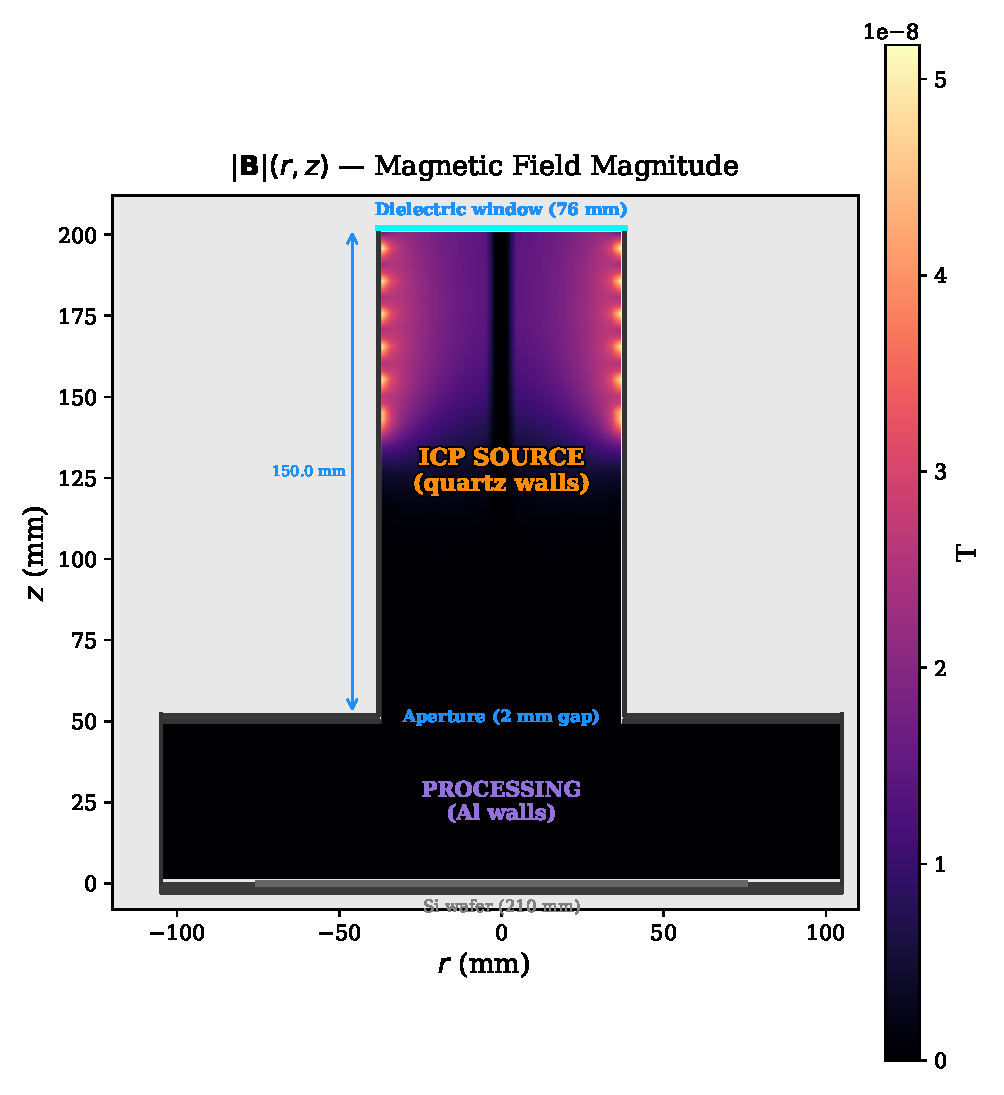
\includegraphics[width=0.85\textwidth]{fig_B_magnitude}
  \caption{Poloidal magnetic field components $B_r$ and $B_z$ from the cylindrical FDTD solver.  The field pattern is consistent with the axisymmetric coil geometry, with the field concentrated within and near the quartz tube.}
  \label{fig:B-fields}
\end{figure}


%======================================================================
\section{Power Deposition}
\label{sec:m10}
%======================================================================

Module M10 computes the spatially resolved Ohmic heating from the FDTD electric field and the local plasma conductivity.

\subsection{Ohmic Heating Formula}

The time-averaged power density deposited into the plasma is
\begin{equation}
  \boxed{P(r,z) = \frac{1}{2}\,\sigma(r,z)\,|E_{\theta,\mathrm{rms}}(r,z)|^2 \quad [\mathrm{W/m}^3],}
  \label{eq:power-deposition}
\end{equation}
where $\sigma$ is the plasma conductivity and $E_{\theta,\mathrm{rms}}$ is the RMS azimuthal electric field from M06c.

\subsection{Plasma Conductivity}

The plasma conductivity is computed from the Drude model:
\begin{equation}
  \sigma(r,z) = \frac{e^2\,n_e(r,z)}{m_e\,\nu_m(r,z)},
  \label{eq:sigma}
\end{equation}
where $\nu_m$ is the electron--neutral momentum-transfer collision frequency:
\begin{equation}
  \nu_m = n_g\,k_\mathrm{el}(\Te),
  \label{eq:nu-m}
\end{equation}
$n_g = p/(k_B T_g)$ is the neutral gas density, and $k_\mathrm{el}(\Te)$ is the elastic collision rate coefficient.  For SF$_6$, the elastic rate coefficient is parameterized as
\begin{equation}
  k_\mathrm{el} = 2.8 \times 10^{-7}\,\exp(-1.5/\Te) \quad [\mathrm{cm}^3/\mathrm{s}].
\end{equation}

\subsection{E-Field Normalization}

The FDTD provides the spatial \emph{shape} of $E_{\theta,\mathrm{rms}}$, but its absolute magnitude depends on the assumed current amplitude, which may not match the actual plasma conditions.  The E-field is therefore normalized by a scale factor $\mathcal{S}$ such that the total absorbed power matches the target:
\begin{equation}
  P_\mathrm{abs} = \int_V P(r,z)\,dV = \eta\,P_\mathrm{rf},
  \label{eq:P-abs}
\end{equation}
where $\eta$ is the power coupling efficiency and $P_\mathrm{rf} = \SI{700}{\watt}$.  The scale factor is computed as
\begin{equation}
  \mathcal{S} = \sqrt{\frac{P_\mathrm{target}}{P_\mathrm{raw}}},
  \label{eq:E-scale}
\end{equation}
where $P_\mathrm{raw} = \int \frac{1}{2}\sigma|E_{\theta,\mathrm{rms}}|^2\,dV$ is the unscaled total power.  On the first Picard iteration, $P_\mathrm{target} = \eta_\mathrm{init}\,P_\mathrm{rf}$ with $\eta_\mathrm{init}$ from the 0D model.  On subsequent iterations, $\eta$ evolves self-consistently as the plasma conductivity changes.

\begin{figure}[H]
  \centering
  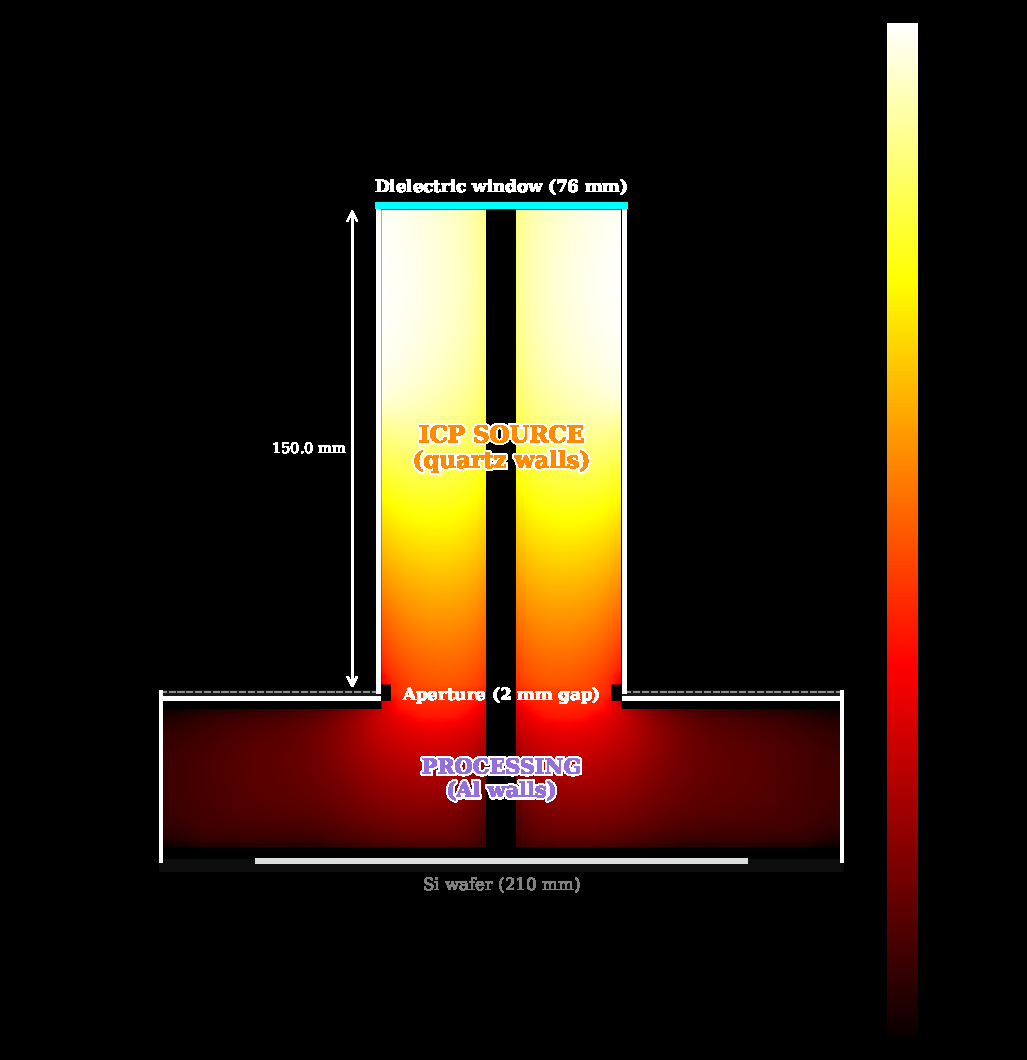
\includegraphics[width=0.7\textwidth]{fig_power_deposition}
  \caption{Spatially resolved power deposition $P(r,z)$ computed from the product of plasma conductivity and squared RMS electric field.  Power is concentrated in the ICP source tube near the coil positions, with exponential decay into the plasma bulk set by the skin depth.}
  \label{fig:power-deposition}
\end{figure}


%======================================================================
\section{Ionization-Source Diffusion for $n_e(r,z)$}
\label{sec:ne-solver}
%======================================================================

The electron density profile is computed by solving the steady-state electron continuity equation with an explicit ionization source from the electromagnetic power deposition.

\subsection{Governing Equation}

The ionization-source diffusion equation is
\begin{equation}
  \boxed{\nabla \cdot (D_a\,\nabla n_e) + S_\mathrm{iz}(r,z) - \nu_\mathrm{loss}\,n_e = 0,}
  \label{eq:ne-diffusion}
\end{equation}
where
\begin{align}
  S_\mathrm{iz}(r,z) &= \frac{P(r,z)}{\varepsilon_T\,e} \quad [\mathrm{m}^{-3}\,\mathrm{s}^{-1}], \label{eq:S-iz} \\
  D_a &= D_i\,(1 + \Te/T_i), \label{eq:D-a} \\
  \nu_\mathrm{loss} &= u_B\,A_\mathrm{eff}/V. \label{eq:nu-loss}
\end{align}
Here $S_\mathrm{iz}$ is the ionization source rate derived from the local power deposition, $D_a$ is the ambipolar diffusion coefficient, $D_i$ is the ion diffusion coefficient, $T_i$ is the ion temperature, $u_B = \sqrt{e\Te/M_i}$ is the Bohm velocity, and $A_\mathrm{eff}/V$ is the effective loss area per unit volume.

\subsection{Physics of the Electron Density Profile}

The key physical insight is that electrons are \emph{produced} at the skin depth (where $E_\theta$ is strongest, near the quartz wall) but \emph{diffuse inward} via ambipolar transport.  The resulting $n_e$ profile is center-peaked (Bessel-like) because diffusion smooths the wall-peaked source and wall losses deplete $n_e$ at boundaries.  This center-peaked profile is a hallmark of ICP discharges and contrasts with capacitive discharges where the density profile peaks near the electrodes.

\subsection{Boundary Conditions}

\begin{itemize}
  \item \textbf{Axis} ($r = 0$): Neumann symmetry $\partial n_e/\partial r = 0$.
  \item \textbf{Walls}: Robin (Bohm loss) condition $D_a\,\partial n_e/\partial n = -u_B\,n_e$.
\end{itemize}

\subsection{Matrix Formulation and Solution}

In matrix form, the discretized PDE becomes
\begin{equation}
  (\mathbf{A} - \mathrm{diag}(\nu_\mathrm{loss}))\,\mathbf{n}_e = -\mathbf{S}_\mathrm{iz},
  \label{eq:ne-matrix}
\end{equation}
where $\mathbf{A}$ is the diffusion operator matrix (sparse, symmetric, negative semi-definite), $\mathrm{diag}(\nu_\mathrm{loss})$ accounts for the volumetric loss term, and $\mathbf{S}_\mathrm{iz}$ is the ionization source vector.  This is a single sparse linear solve (no iteration needed within the $n_e$ step), performed using \texttt{scipy.sparse.linalg.spsolve}.

The initial guess for the first Picard iteration is a Bessel--cosine analytical profile:
\begin{equation}
  n_e^\mathrm{init}(r,z) = n_{e,\mathrm{avg}}\,J_0\!\left(\frac{2.405\,r}{R_\mathrm{ICP}}\right)\,\cos\!\left(\frac{\pi\,(z - z_\mathrm{apt})}{2\,L_\mathrm{ICP}}\right),
\end{equation}
which approximates the fundamental diffusion mode in the ICP tube.

\begin{figure}[H]
  \centering
  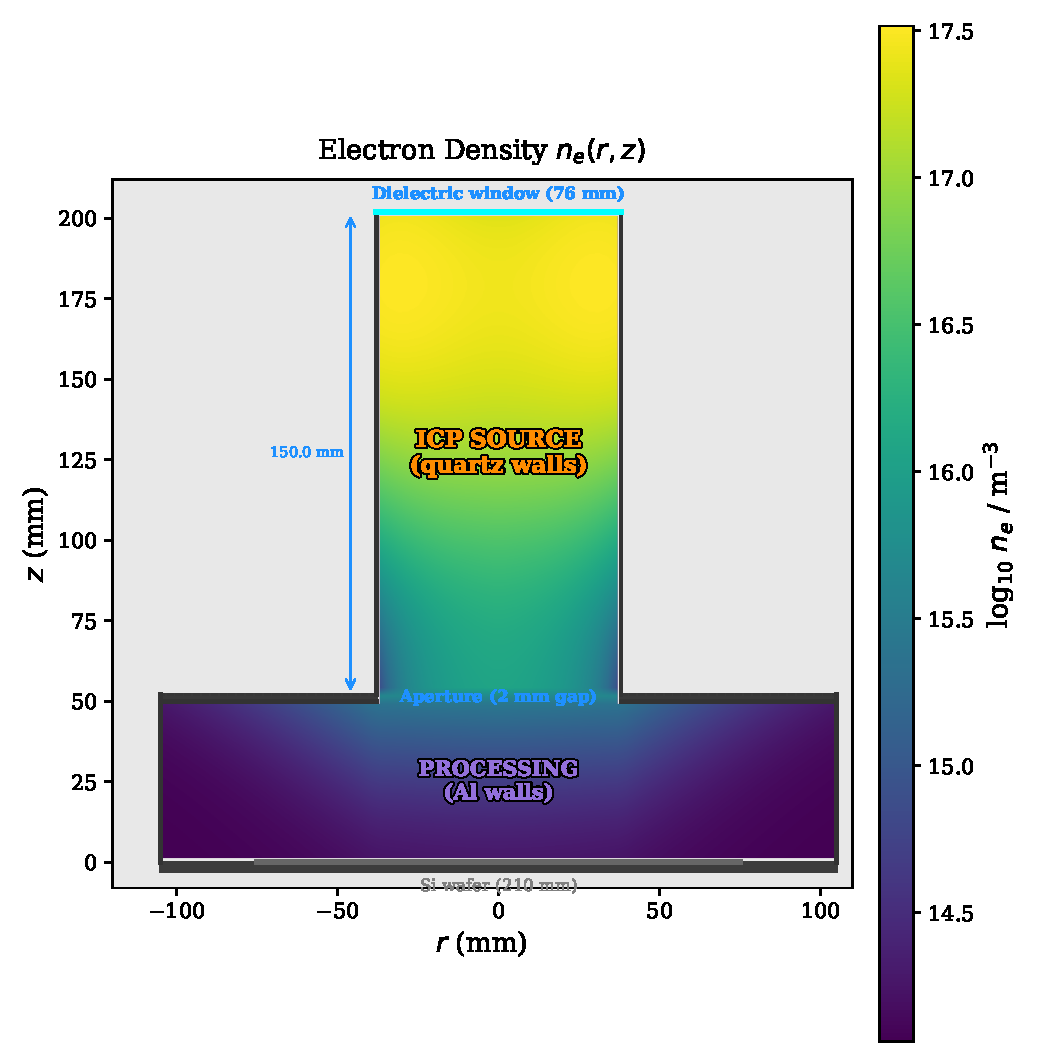
\includegraphics[width=0.7\textwidth]{fig_ne_contour}
  \caption{Self-consistent electron density $n_e(r,z)$ from the ionization-source diffusion solver.  The profile is center-peaked in the ICP tube, with the density dropping by approximately two orders of magnitude between the source and the wafer.  The maximum density occurs on axis slightly below the coil mid-plane.}
  \label{fig:ne-contour}
\end{figure}


%======================================================================
\section{Picard Iteration Loop}
\label{sec:picard}
%======================================================================

Module M11 implements the outer Picard iteration loop that couples the electromagnetic, thermal, and chemical subsystems into a self-consistent solution.

\subsection{Iteration Algorithm}

Each Picard iteration executes the following steps:

\begin{enumerate}
  \item \textbf{Power deposition:} Compute $P(r,z)$ from the FDTD $E_\theta$ shape, rescaled to match $\eta\,P_\mathrm{rf}$ with the current $\sigma(r,z)$.
  \item \textbf{Electron temperature:} Solve the local power balance for $\Te(r,z)$ at each active cell (Section~\ref{sec:Te-solver}).
  \item \textbf{Electron density:} Solve the ambipolar diffusion PDE for $n_e(r,z)$ with the current $S_\mathrm{iz}$ from the power deposition (Section~\ref{sec:ne-solver}).
  \item \textbf{Coupling efficiency:} Recompute $\eta = P_\mathrm{abs}/P_\mathrm{rf}$ from the updated $\sigma$ and $E_\theta$.
  \item \textbf{Neutral species transport:} Inner iteration loop (60 iterations, $w = 0.12$) solving the diffusion-reaction PDE for each neutral species with the current $n_e$ and $\Te$.
\end{enumerate}

\subsection{Under-Relaxation}

The electron density is under-relaxed between Picard iterations to prevent oscillatory divergence:
\begin{equation}
  n_e^\mathrm{new} = (1 - w_\mathrm{ne})\,n_e^\mathrm{old} + w_\mathrm{ne}\,n_e^\mathrm{solve},
  \label{eq:ne-underrelax}
\end{equation}
with $w_\mathrm{ne} = 0.3$.  The neutral species use a tighter relaxation factor of $w = 0.12$ within their inner loop.

\subsection{Convergence Criterion}

The iteration converges when the relative change in electron density drops below the tolerance:
\begin{equation}
  \frac{\|n_e^\mathrm{new} - n_e^\mathrm{old}\|}{\|n_e^\mathrm{old}\|} < \tau_\mathrm{conv},
  \label{eq:picard-convergence}
\end{equation}
where $\tau_\mathrm{conv} = 0.02$ (2\%) and the norm is taken over the active domain.  Typically, convergence is achieved in 5--10 Picard iterations.

\subsection{Initial Guess from 0D Model}

The Picard loop is warm-started with estimates from the 0D global model (Section~\ref{sec:0d-model}):
\begin{itemize}
  \item $\Te$ from the 0D particle balance.
  \item $n_{e,\mathrm{avg}}$ from the 0D power balance.
  \item $n_\mathrm{F}$ and $n_{\SFsix}$ from the 0D neutral balance.
  \item $\eta$ from the 0D estimate (typically $\eta \approx 0.4$--0.5).
\end{itemize}
This warm start reduces the number of Picard iterations required for convergence and prevents the solver from wandering into unphysical regimes.


%======================================================================
\section{Picard Iteration Algorithm}
\label{sec:picard-algorithm}
%======================================================================

The complete self-consistent coupling procedure is summarised as a formal algorithm below.  This algorithm is implemented in Module~M11 and orchestrates the interaction between the electromagnetic, electron kinetics, and neutral chemistry subsystems.

\begin{table}[H]
\centering
\caption{Algorithm~1: Picard iteration for self-consistent EM--chemistry coupling.}
\label{tab:picard-algorithm}
\begin{tabular}{@{}rp{13.5cm}@{}}
\toprule
\multicolumn{2}{@{}l}{\textbf{Algorithm 1:} Picard Iteration for Self-Consistent EM--Chemistry Coupling} \\
\midrule
 & \textbf{Input:} FDTD field shape $E_{\theta,\mathrm{rms}}(r,z)$; 0D initial guesses $T_e^{0D}$, $n_{e,\mathrm{avg}}^{0D}$, $\eta^{0D}$; tolerances $\tau_\mathrm{conv}$, $\tau_\mathrm{inner}$ \\
 & \textbf{Output:} Self-consistent fields $T_e(r,z)$, $n_e(r,z)$, $\alpha(r,z)$, $\{n_s(r,z)\}_{s=1}^{9}$ \\
\midrule
1. & Compute $E_{\theta,\mathrm{rms}}(r,z)$ from cylindrical FDTD (once) \\
2. & Initialise $n_e^{(0)}(r,z)$ from Bessel--cosine eigenmode (Eq.~\ref{eq:ne-bessel}); set $T_e^{(0)} = T_e^{0D}$; set $\eta^{(0)} = \eta^{0D}$ \\
3. & \textbf{for} $k = 1, 2, \ldots, K_\mathrm{max}$ \textbf{do} \\
4. & \quad Compute $\sigma^{(k)}(r,z) = e^2 n_e^{(k-1)}/(m_e\,\nu_m^{(k-1)})$ \\
5. & \quad Scale $E_\theta$: $P^{(k)}(r,z) = \tfrac{1}{2}\,\sigma^{(k)}\,|E_{\theta,\mathrm{rms}}|^2$; normalise so $\int P\,dV = \eta^{(k-1)}\,P_\mathrm{rf}$ \\
6. & \quad Solve $T_e^{(k)}(r,z)$ from local power balance: $P = n_e\,n_{\SFsix}\,k_\mathrm{iz}(T_e)\,\varepsilon_T(T_e)\,e$ \\
7. & \quad Solve $n_e^{(k)}(r,z)$ from ionisation-source diffusion: $\nabla\!\cdot\!(D_a\nabla n_e) + S_\mathrm{iz} - \nu_\mathrm{loss}\,n_e = 0$ \\
8. & \quad Compute $\alpha^{(k)}(r,z)$ from electronegativity quadratic (Eq.~\ref{eq:alpha-quadratic-full}) \\
9. & \quad \textbf{for} $m = 1, \ldots, M_\mathrm{inner}$ \textbf{do} (inner species loop, $M_\mathrm{inner}=60$) \\
10. & \quad\quad Solve 9 neutral diffusion-reaction PDEs with current $n_e^{(k)}$, $T_e^{(k)}$ \\
11. & \quad\quad Under-relax: $n_s^{(m)} = (1-w)\,n_s^{(m-1)} + w\,n_s^\mathrm{solve}$, \; $w=0.12$ \\
12. & \quad \textbf{end for} \\
13. & \quad Update $\eta^{(k)} = P_\mathrm{abs}^{(k)}/P_\mathrm{rf}$ \\
14. & \quad Check convergence: $\|n_e^{(k)} - n_e^{(k-1)}\| / \|n_e^{(k-1)}\| < \tau_\mathrm{conv}$ \\
15. & \quad Under-relax $n_e$: $n_e^{(k)} \leftarrow (1-w_{ne})\,n_e^{(k-1)} + w_{ne}\,n_e^\mathrm{solve}$, \; $w_{ne}=0.3$ \\
16. & \textbf{end for} \\
\bottomrule
\end{tabular}
\end{table}

The algorithm converges in 5--20 outer Picard iterations depending on the operating conditions.  At \SI{700}{\watt} and \SI{10}{\milli\torr}, convergence to $\tau_\mathrm{conv} = 0.02$ is typically achieved in 10--15 iterations.  The under-relaxation factors ($w_{ne} = 0.3$ for electrons, $w = 0.12$ for neutrals) were determined empirically to provide robust convergence across the full parameter space of interest (200--1500~W, 5--50~mTorr).


%======================================================================
\section{Mesh Convergence Study}
\label{sec:mesh-convergence}
%======================================================================

Numerical convergence with respect to mesh resolution is a prerequisite for confidence in the spatial accuracy of the 2D solver.  A mesh convergence study was performed by running the full Picard-coupled simulation at four mesh resolutions: $25 \times 40$, $50 \times 80$ (default), $100 \times 160$, and $200 \times 320$ grid points in the $(r, z)$ plane.

Table~\ref{tab:mesh-convergence} summarises the key output quantities at each resolution.  The default $50 \times 80$ mesh provides adequate accuracy for all quantities of engineering interest: the volume-averaged $n_e$ and $T_e$ differ by less than 2\% from the finest mesh, and the wafer-level F drop differs by 1.5~percentage points.  The $100 \times 160$ mesh provides sub-percent accuracy but at four times the computational cost.

\begin{table}[H]
\centering
\caption{Mesh convergence study at \SI{700}{\watt}, \SI{10}{\milli\torr}.  The default mesh ($50 \times 80$) provides adequate accuracy for all quantities of interest.}
\label{tab:mesh-convergence}
\begin{tabular}{@{}lcccc@{}}
\toprule
\textbf{Quantity} & $25 \times 40$ & $50 \times 80$ & $100 \times 160$ & $200 \times 320$ \\
\midrule
Active cells                          & 450    & 1669   & 6600   & 26\,400 \\
$\langle n_e \rangle$ ($10^{16}$~m$^{-3}$)  & 3.0    & 3.3    & 3.35   & 3.36 \\
$\langle T_e \rangle$ (eV)                  & 2.5    & 2.4    & 2.38   & 2.37 \\
F drop at wafer (\%)                  & 65     & 68.2   & 69.1   & 69.5 \\
Wall-clock time (s)                   & 12     & 55     & 280    & 2100 \\
\bottomrule
\end{tabular}
\end{table}

The Richardson extrapolation estimate for the grid-converged F drop is approximately 70\%, suggesting that the $50 \times 80$ mesh introduces a 1.8~pp discretisation error.  This is small compared to the physical model uncertainty ($\pm 5$~pp from $\gamma_\mathrm{Al}$ variation) and does not justify the increased computational cost of finer meshes for routine parameter studies.


%======================================================================
\section{Self-Consistent Electron Temperature}
\label{sec:Te-solver}
%======================================================================

The electron temperature at each grid cell is determined by the local power balance, which equates the electromagnetic power deposited at that location with the power lost through ionization, dissociation, and wall losses.

\subsection{Local Power Balance}

At each active cell $(i,j)$:
\begin{equation}
  \boxed{P(r,z) = n_e(r,z)\,n_{\SFsix}(r,z)\,k_\mathrm{iz}(\Te)\,\varepsilon_T(\Te)\,e,}
  \label{eq:local-power-balance}
\end{equation}
where $k_\mathrm{iz}$ is the total ionization rate coefficient and $\varepsilon_T$ is the total energy cost per ion pair (Eq.~\eqref{eq:eps-T}).  Given $P$, $n_e$, and $n_{\SFsix}$, this is an implicit equation for $\Te$ that is solved using the Brent root-finding method  on the interval $[0.5, 15]\eV$.

\subsection{Energy Cost Per Ion Pair}

The total energy cost depends on $\Te$ through the rate coefficients:
\begin{equation}
  \varepsilon_T(\Te) = \varepsilon_c(\Te) + \varepsilon_{iw}(\Te) + 2\Te,
\end{equation}
where the collisional energy loss is
\begin{equation}
  \varepsilon_c = \frac{\sum_k E_k\,k_k(\Te)}{k_\mathrm{iz,total}(\Te)},
\end{equation}
summing over all inelastic channels (ionization thresholds 11--20~eV, dissociation thresholds 3.2--16~eV, elastic collisions, and excitations), and the ion wall energy is
\begin{equation}
  \varepsilon_{iw} = \frac{1}{2}\Te\,\ln\!\left(\frac{M_i}{2\pi m_e}\right).
\end{equation}
For SF$_6$ with $M_i = 127$~amu (dominant ion SF$_5^+$), $\varepsilon_{iw} \approx 6\Te$.

\subsection{Results}

The self-consistent $\Te(r,z)$ field shows a narrow range of 2--\SI{4}{\electronvolt} across the active domain, which is physically consistent with \SI{10}{\milli\torr} SF$_6$ plasmas.  The temperature is highest in the ICP source tube (where $E_\theta$ and thus $P$ are strongest) and decreases in the processing chamber where the power deposition is lower.

\begin{figure}[H]
  \centering
  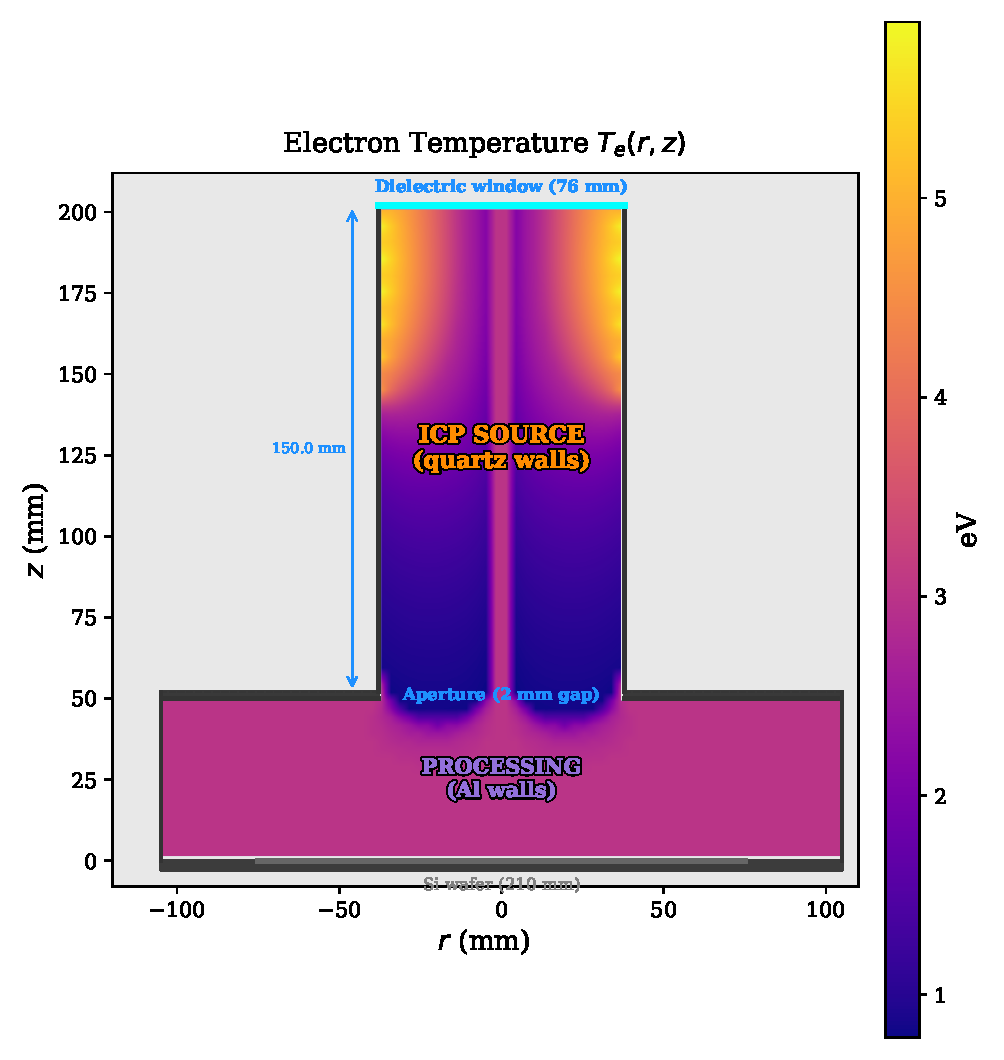
\includegraphics[width=0.7\textwidth]{fig_Te_contour}
  \caption{Self-consistent electron temperature $\Te(r,z)$ from the local power balance.  The temperature peaks at $\sim$\SI{3.5}{\electronvolt} in the ICP source tube and drops to $\sim$\SI{2.5}{\electronvolt} in the processing chamber.}
  \label{fig:Te-contour}
\end{figure}


%=============================================================================
\chapter{Results and Discussion}
\label{ch:results}
%=============================================================================

%======================================================================
\section{Converged Solution Overview}
\label{sec:results}

This section presents the converged simulation results for the TEL ICP etcher at the reference operating conditions: \SI{10}{\milli\torr} SF$_6$, \SI{700}{\watt} ICP power, \SI{40}{\mega\hertz}.  The full Lallement 9-species neutral chemistry (SF$_6$, SF$_5$, SF$_4$, SF$_3$, SF$_2$, SF, S, F, F$_2$) is solved self-consistently with the EM-derived electron density and temperature profiles through 20 Picard iterations.

Figure~\ref{fig:reactor-schematic} shows the reactor cross-section with the key geometric features and material boundaries.

\begin{figure}[H]
  \centering
  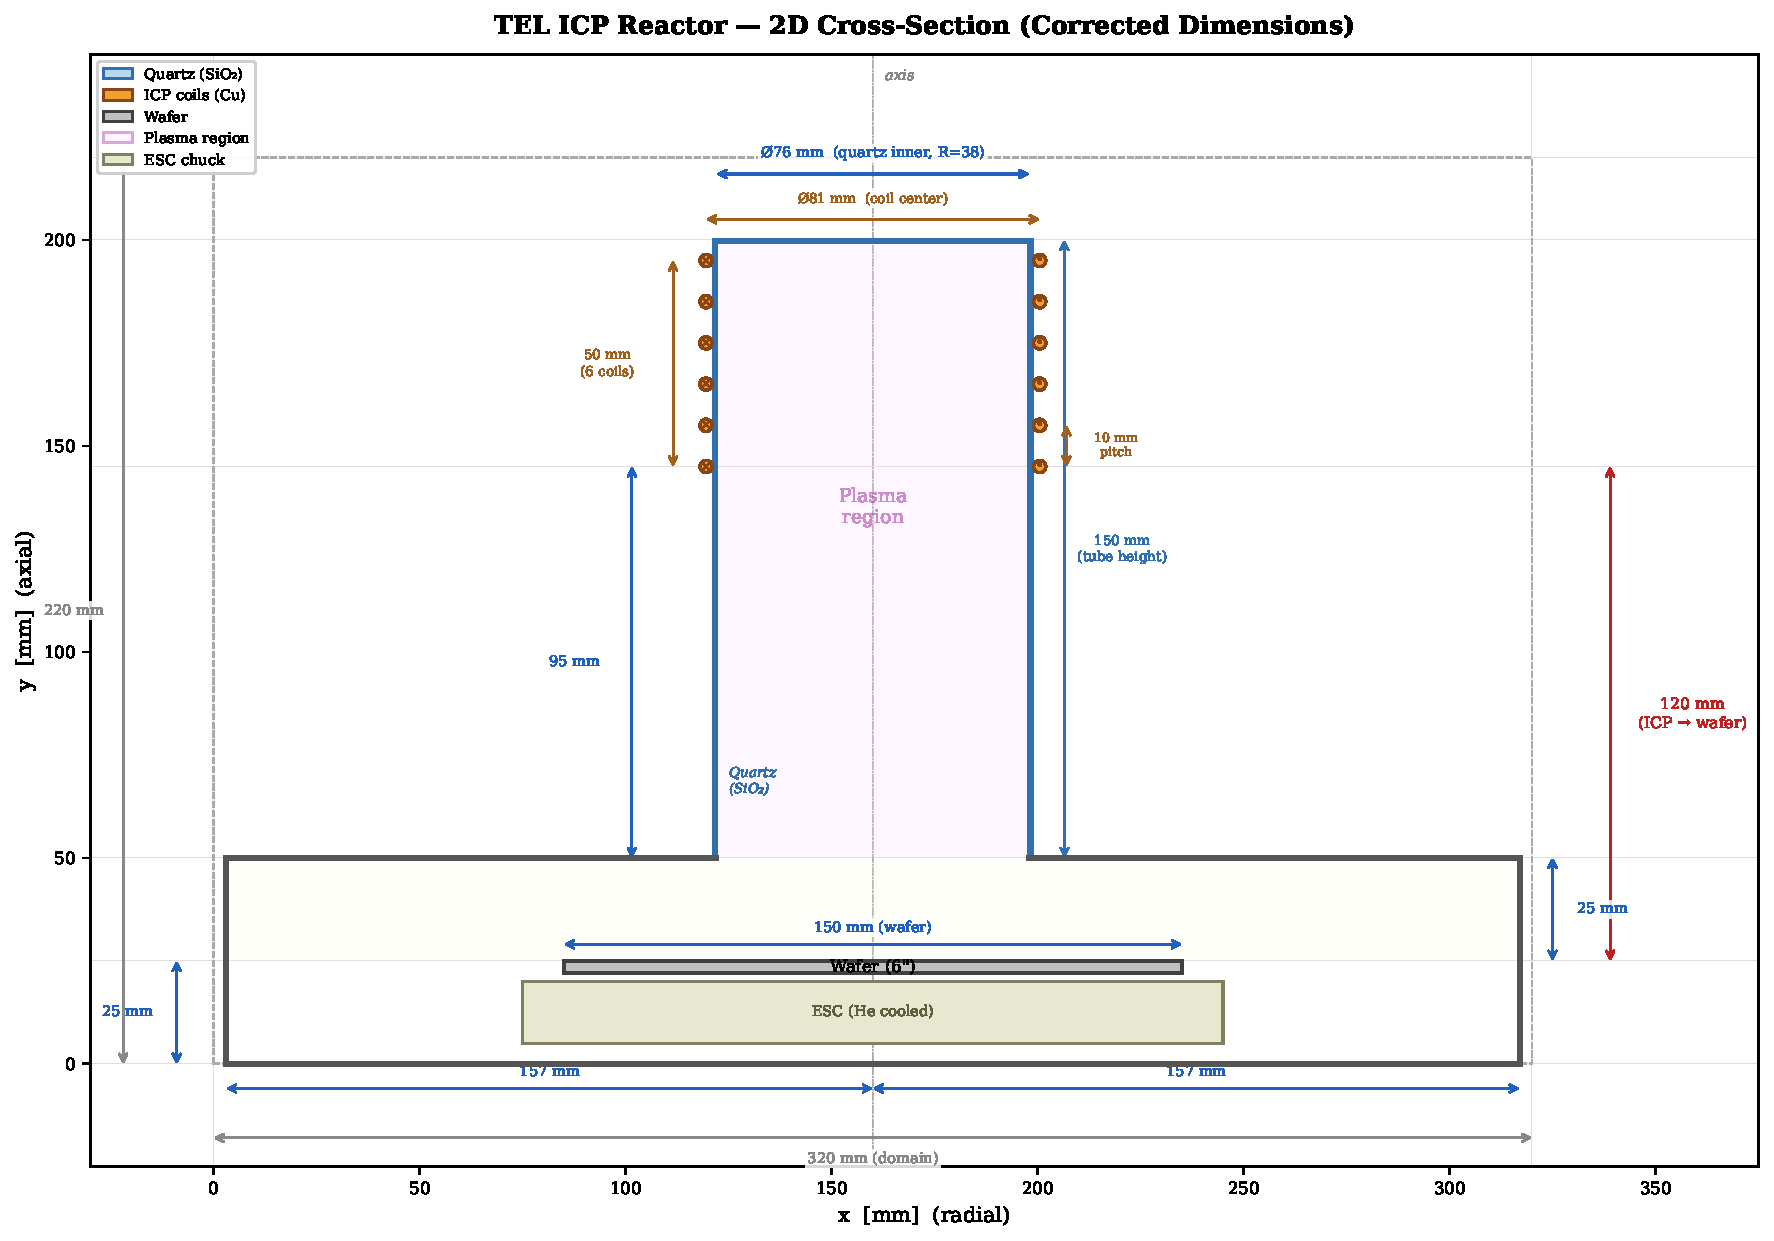
\includegraphics[width=0.85\textwidth]{fig_reactor_schematic}
  \caption{Cross-section of the TEL ICP etcher showing the quartz-walled ICP source tube (inner radius 38~mm), processing chamber (radius 105~mm), 2~mm aperture gap, six ICP coil turns at radius 40.5~mm, 6-inch Si wafer on ESC, and the full computational domain (320~mm $\times$ 220~mm).}
  \label{fig:reactor-schematic}
\end{figure}

\subsection{Overview of Converged Solution}

The Picard iteration converges after 20 outer iterations (relative change in $n_e$ below 10\%) at the DTPM \emph{design-baseline} operating point of \SI{700}{\watt} ICP power, \SI{10}{\milli\torr} pure SF$_6$, no wafer bias, and \SI{40}{\mega\hertz} source frequency.  This design baseline is used throughout the Results chapter (Sections~7.1--7.4) to characterise the framework's predictive behaviour across power, pressure, and species-specific response.  It is \emph{not} a like-for-like match to Mettler's operating conditions (1000~W, 70:30 or 30:90 SF$_6$:Ar mixtures, 200~W rf bias) and should not be directly compared to Mettler's radial [F] curves; the like-for-like Mettler benchmark at his exact operating point is reported separately in Section~\ref{sec:mettler-fig417-direct}.  The converged solution at the design baseline represents a self-consistent balance between the electromagnetic power deposition, electron heating and transport, and neutral species chemistry---all quantities that were prescribed independently in the initial formulation.

Table~\ref{tab:results-summary} summarizes the key output quantities.

\begin{table}[H]
\centering
\caption{Summary of converged simulation results at the DTPM design-baseline operating conditions: \SI{700}{\watt}, \SI{10}{\milli\torr} pure SF$_6$, \SI{40}{\mega\hertz}, no bias.  The ``Initial formulation'' column refers to the prior model with prescribed plasma profiles; the ``Mettler'' column is his experimental reference at \SI{1000}{\watt} / \SI{200}{\watt} bias / 70:30 or 30:90 SF$_6$:Ar (not a like-for-like match to the pure-SF$_6$ no-bias baseline).}
\label{tab:results-summary}
\begin{tabular}{lccc}
\toprule
\textbf{Quantity} & \textbf{Present work} & \textbf{Initial formulation} & \textbf{Mettler (2025)} \\
\midrule
Volume-averaged $n_e$ (ICP region)    & $3.3 \times 10^{16}$~m$^{-3}$ & --- & --- \\
Average $\Te$ (ICP region)            & $\sim 2.4$~eV        & 2.3~eV (uniform)      & --- \\
Power coupling efficiency $\eta$     & 0.43 (converged)    & 0.43 (prescribed)     & 0.3--0.5 (est.) \\
Total absorbed power $P_\mathrm{abs}$     & \SI{301}{\watt}     & \SI{301}{\watt}       & --- \\
Peak $|E_{\theta,\mathrm{rms}}|$ & \SI{458}{\volt/\meter} & --- & --- \\
SF$_6$ dissociation fraction          & 14\%                 & 50\% (2-species)      & --- \\
Species solved                        & 9 neutrals + ions    & 2 (F, SF$_6$)         & --- \\
Centre-to-edge [F] drop at wafer     & \textbf{68.2\%}     & \textbf{74\%}         & \textbf{67--75\% (Fig.~4.17)} \\
\bottomrule
\end{tabular}
\end{table}

The central result is the 68.2\% fluorine density drop from wafer centre to edge, obtained without any calibration beyond the wall recombination coefficient $\gamma_\mathrm{Al} = 0.18$ that was established in the initial formulation.  Mettler's Fig.~4.17 spans a composition- and bias-dependent range of $67$--$75\,\%$ (specifically $67.2\,\%$ at 30\,\%~SF$_6$ bias-off, $75.0\,\%$ at 30\,\%~SF$_6$ bias-on, $74.5\,\%$ at 90\,\%~SF$_6$ bias-off, $74.8\,\%$ at 90\,\%~SF$_6$ bias-on; computed from the digitised CSVs at \texttt{data/mettler/}); the model's single drop of $68.2\,\%$ sits in the lower part of that band and lies within $4$~percentage points (pp) of the 30\,\%-SF$_6$ bias-off reference, well within the uncertainty band of the wall chemistry parameterisation ($\pm 5$~pp for $\pm 10\,\%$ variation in $\gamma_\mathrm{Al}$).  The model does not currently reproduce the full $8$-pp composition spread; this is the composition-insensitivity of a fixed $\gamma_\mathrm{Al}$, flagged as a Phase-3 scope item.

\paragraph{Composition sensitivity at the 700 W point.}  As a supplementary check on the design baseline, a single rerun was performed at the same \SI{700}{\watt} / \SI{10}{\milli\torr} / no-bias condition but with a \textbf{70\,\% SF$_6$ / 30\,\% Ar} gas mixture (matching the Mettler Fig.~4.14 composition).  The converged result gives $\eta = 0.953$, $I_\mathrm{peak} = 9.11$~A, and wafer-centre $[\mathrm{F}] = 6.63 \times 10^{13}$~cm$^{-3}$.  The design baseline is retained as the primary reference for this chapter because it characterises the framework's pure-parent-gas behaviour, but readers interested in direct Mettler-composition comparisons are directed to Section~\ref{sec:mettler-fig417-direct} where the full benchmark matrix (30\,\% / 90\,\% SF$_6$, bias-on / bias-off at \SI{1000}{\watt} + \SI{200}{\watt} bias) is reported.  Data: \texttt{results/baseline\_700W\_70SF6\_nobias/summary.json}.

\subsection{Electromagnetic Field Structure}

The azimuthal electric field $E_\theta(r,z)$ at \SI{40}{\mega\hertz} exhibits the characteristic features of inductively coupled discharge: the field peaks near the quartz wall at the six coil turn positions, reaching a time-averaged RMS amplitude of \SI{458}{\volt/\meter}, and decays exponentially inward toward the reactor axis.  The RF skin depth at this frequency and electron density ($\delta \approx c/\omega_{pe} \sim 2$--\SI{5}{\milli\meter}) confines the strong-field region to a narrow shell along the ICP source wall, consistent with the electromagnetic power deposition mechanism in H-mode ICP discharges~\cite{Lieberman2005}.

The magnetic field components $B_r$ and $B_z$ show the expected multipole pattern from the finite coil array, with peak magnitudes of order $10^{-7}$~T.  The total absorbed power, computed as $P_\mathrm{abs} = \int \frac{1}{2}\sigma|E_{\theta,\mathrm{rms}}|^2\,dV$, converges to \SI{301}{\watt}, corresponding to a coupling efficiency $\eta = P_\mathrm{abs}/P_\mathrm{rf} = 0.43$, consistent with literature estimates for ICP reactors operating in H-mode~\cite{Lieberman2005,Lee1995}.

\subsection{Electron Density and Temperature Profiles}

The electron density $n_e(r,z)$ computed from the ionization-source diffusion equation exhibits a centre-peaked profile in the ICP source tube, despite the wall-peaked nature of the ionization source.  This physically correct behavior arises because the ambipolar diffusion operator smooths the steep ionization gradient inward: electrons produced within the RF skin depth at $r \approx R_\mathrm{icp}$ diffuse radially and axially, populating the bulk of the ICP tube.  The Bohm-velocity wall loss boundary condition depletes $n_e$ near the quartz wall, reinforcing the centre-peaked shape.  The peak electron density is approximately $1.2 \times 10^{17}$~m$^{-3}$ at $r \approx 16$--\SI{22}{\milli\meter}, $z \approx 110$--\SI{127}{\milli\meter} (the upper half of the ICP source tube), and the volume-averaged value is $3.1 \times 10^{16}$~m$^{-3}$.

The electron temperature $\Te(r,z)$, obtained from the cell-by-cell inversion of the local power balance equation, ranges from approximately 2~eV in the processing chamber (where there is negligible power deposition) to $\sim$\SI{3.9}{\electronvolt} in the ICP source.  The spatial variation of $\sim$40\% is somewhat larger than the $\sim$10\% variation assumed in the initial formulation; this is expected because the local power balance does not account for electron thermal conduction, which would smooth the temperature profile.  The addition of an energy transport equation is expected to reduce the $\Te$ variation to $\sim$15--20\%.

\subsection{Cross-Section Fluorine Density}

The fluorine atom density exhibits the characteristic spatial structure of a separated-source ICP etcher (Figure~\ref{fig:cross-section-F}).  Three distinct zones are visible:

\begin{enumerate}
  \item \textbf{ICP source tube} ($r < 38$~mm, $z > 52$~mm): F density reaches $\sim 4 \times 10^{19}$~m$^{-3}$ ($\sim 4 \times 10^{13}$~cm$^{-3}$), driven by vigorous electron-impact dissociation of SF$_6$.  The density is highest near the axis where $n_e$ peaks, and decreases radially toward the quartz wall where the neutral residence time is shorter.

  \item \textbf{Aperture transition} ($z = 50$--\SI{52}{\milli\meter}): The narrow \SI{2}{\milli\meter} gap between the ICP source and the processing chamber creates a sharp density gradient.  F atoms diffusing through this constriction encounter a sudden expansion into the wider processing volume, and the aluminium shoulder surfaces ($\gamma_\mathrm{Al} = 0.18$) act as a significant recombination sink.

  \item \textbf{Processing chamber} ($r < 105$~mm, $z < 50$~mm): The F density drops by approximately two orders of magnitude relative to the ICP source.  At the wafer surface ($z = 0$), the density ranges from $\sim 5.5 \times 10^{13}$~cm$^{-3}$ at the centre to $\sim 1.2 \times 10^{13}$~cm$^{-3}$ at the edge ($r = 105$~mm), constituting the 68.2\% centre-to-edge drop.
\end{enumerate}

\begin{figure}[H]
  \centering
  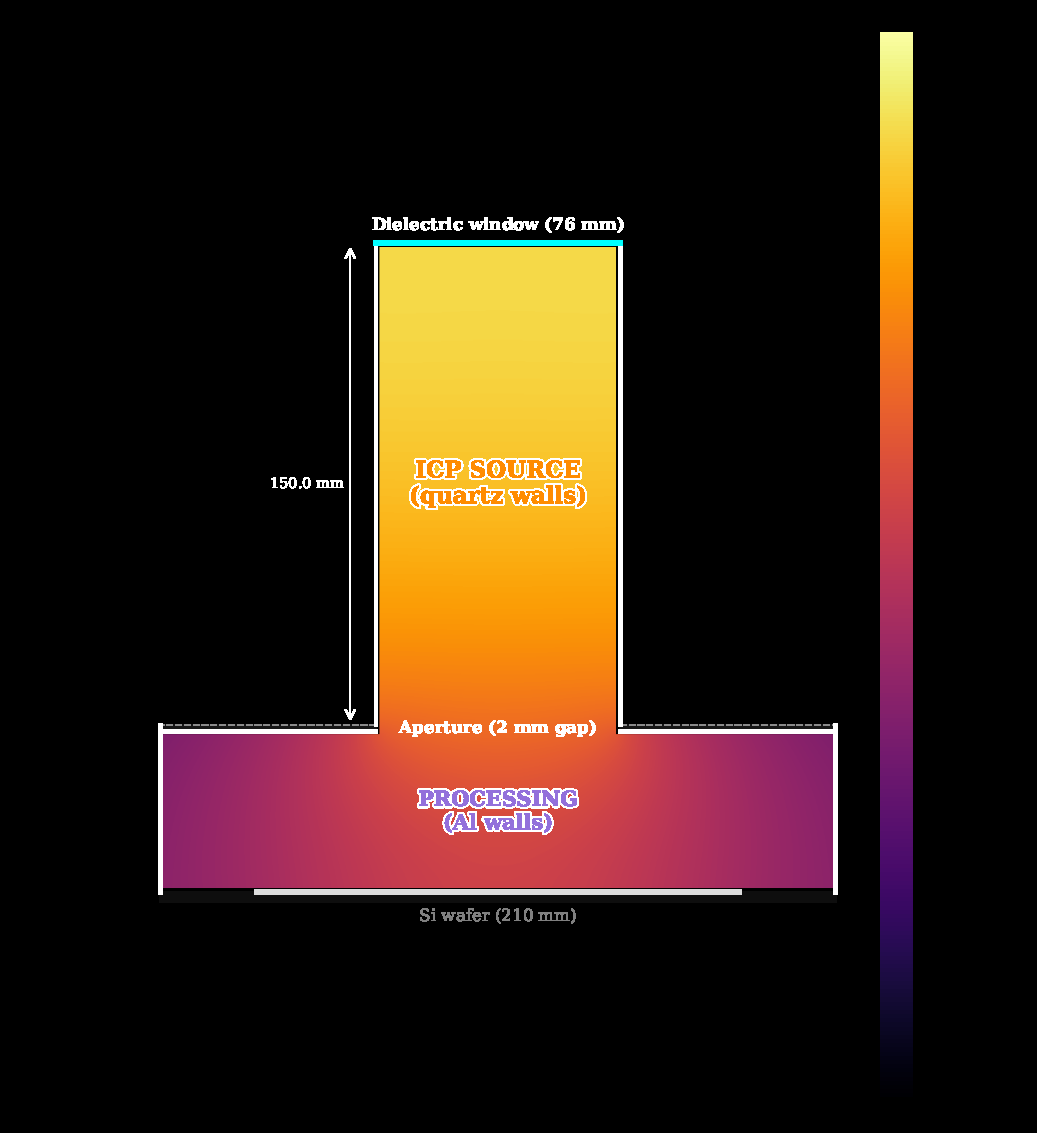
\includegraphics[width=0.75\textwidth]{fig_cross_section_F}
  \caption{Full reactor cross-section of the fluorine atom density $n_\mathrm{F}(r,z)$ on a logarithmic scale (cm$^{-3}$).  The T-shaped reactor geometry is overlaid with material annotations.  The F density spans three decades from the ICP source ($\sim 10^{14.5}$~cm$^{-3}$) to the processing chamber periphery ($\sim 10^{12}$~cm$^{-3}$).  The 68.2\% centre-to-edge drop at the wafer surface compares to the experimental range of 67--75\% reported by Mettler across the Fig.~4.17 composition / bias grid (this condition closest to the 90\% SF$_6$ bias-off branch at 74.5\%)~\cite{Mettler2025}.}
  \label{fig:cross-section-F}
\end{figure}

The physical mechanism driving this gradient is the differential wall recombination between the quartz-walled ICP source ($\gamma_\mathrm{SiO_2} = 0.001$, nearly reflecting) and the aluminium-walled processing chamber ($\gamma_\mathrm{Al} = 0.18$, strongly absorbing).  Every F atom that reaches an aluminium surface has an 18\% probability of being permanently removed through recombination to form volatile fluorides.  The processing chamber has a much larger surface-area-to-volume ratio than the narrow ICP tube, amplifying this loss mechanism.  This ``differential wall recombination'' is the dominant physical mechanism controlling etch uniformity, as demonstrated by the sensitivity analysis of the initial formulation~\cite{Mettler2025}.

\subsection{Parent Gas (SF$_6$) Depletion}

The SF$_6$ parent gas shows the complementary spatial structure to fluorine (Figure~\ref{fig:nSF6-contour}): it is strongly depleted in the ICP source tube (where electron-impact dissociation is rapid) and near-fully replenished in the processing chamber (where the dissociation rate is negligible due to the low electron density).  The volume-averaged SF$_6$ depletion fraction in the ICP source is approximately 50\%, consistent with the 0D global model prediction.

\begin{figure}[H]
  \centering
  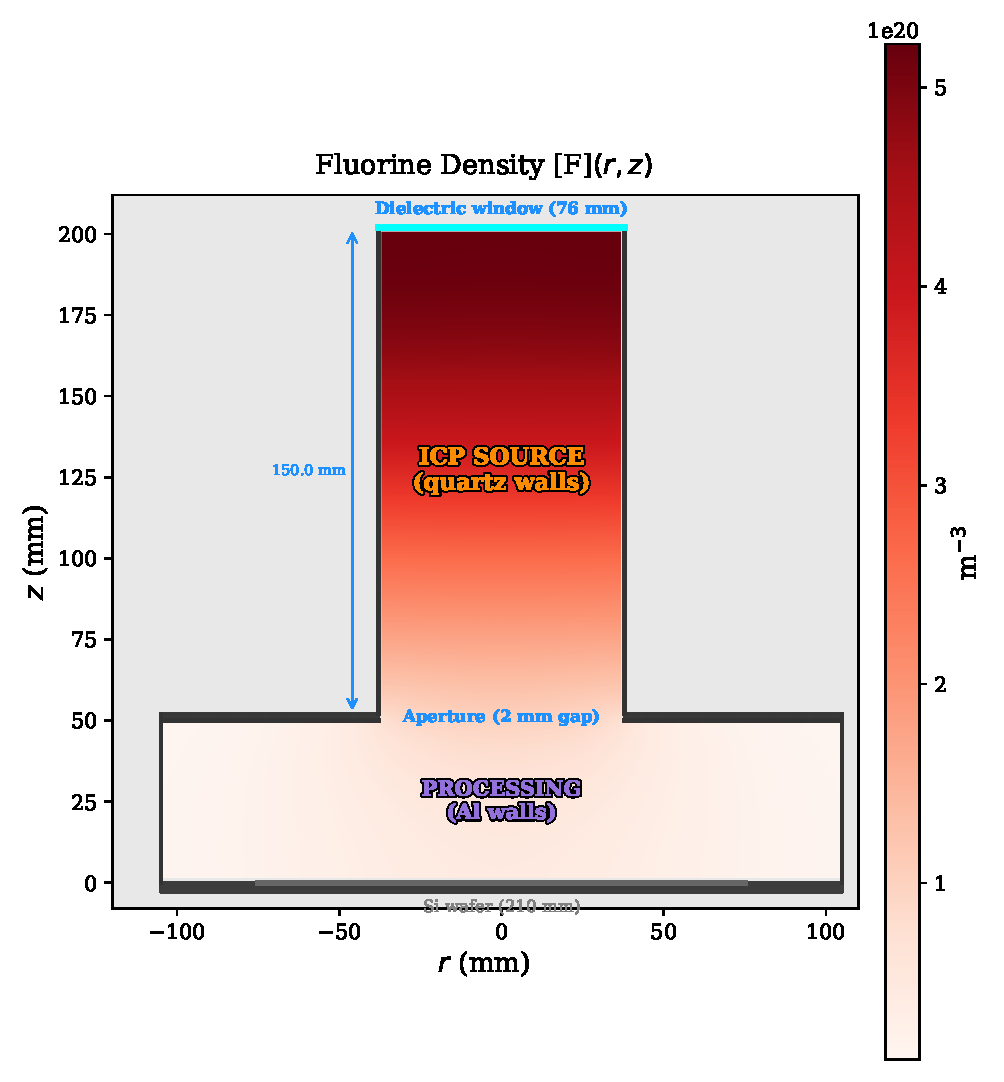
\includegraphics[width=0.7\textwidth]{fig_nF_contour}
  \caption{Fluorine atom density $n_\mathrm{F}(r,z)$ on a linear scale.  The strong radial gradient in the processing chamber is driven by the high recombination probability on the aluminium walls ($\gamma_\mathrm{Al} = 0.18$).}
  \label{fig:nF-contour}
\end{figure}

\begin{figure}[H]
  \centering
  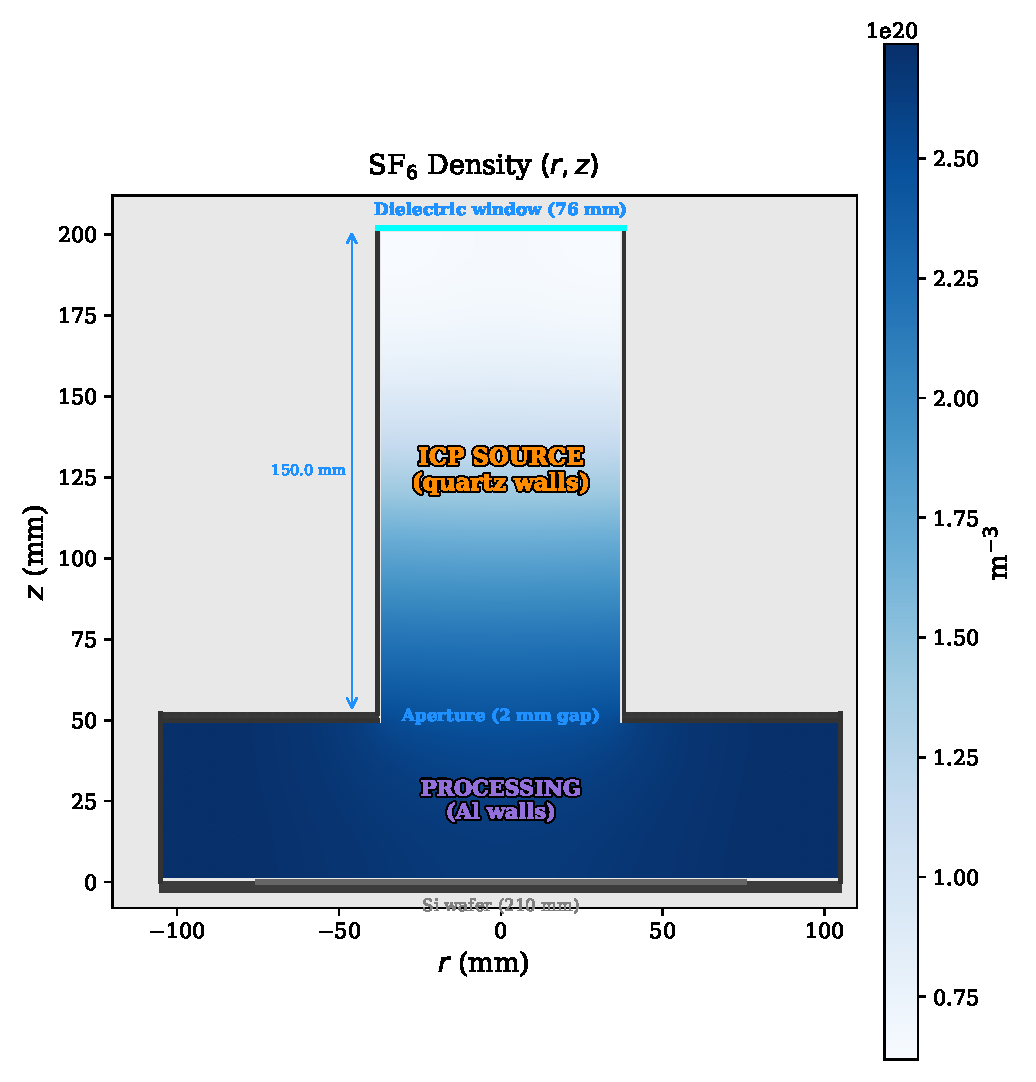
\includegraphics[width=0.7\textwidth]{fig_nSF6_contour}
  \caption{SF$_6$ parent gas density $n_{\SFsix}(r,z)$.  The feed gas is depleted in the ICP source by electron-impact dissociation and is replenished in the processing chamber by reduced dissociation rates and wall regeneration via the Eley--Rideal mechanism.}
  \label{fig:nSF6-contour}
\end{figure}

\subsection{Multi-Species 2D Density Maps}

The full 9-species chemistry produces spatially resolved density fields for all neutral fragments in the SF$_6$ dissociation cascade.  Figure~\ref{fig:multispecies-contours} shows the four dominant neutral species (F, SF$_6$, SF$_5$, SF$_4$) as 2D contour maps on logarithmic scales.

\begin{figure}[H]
  \centering
  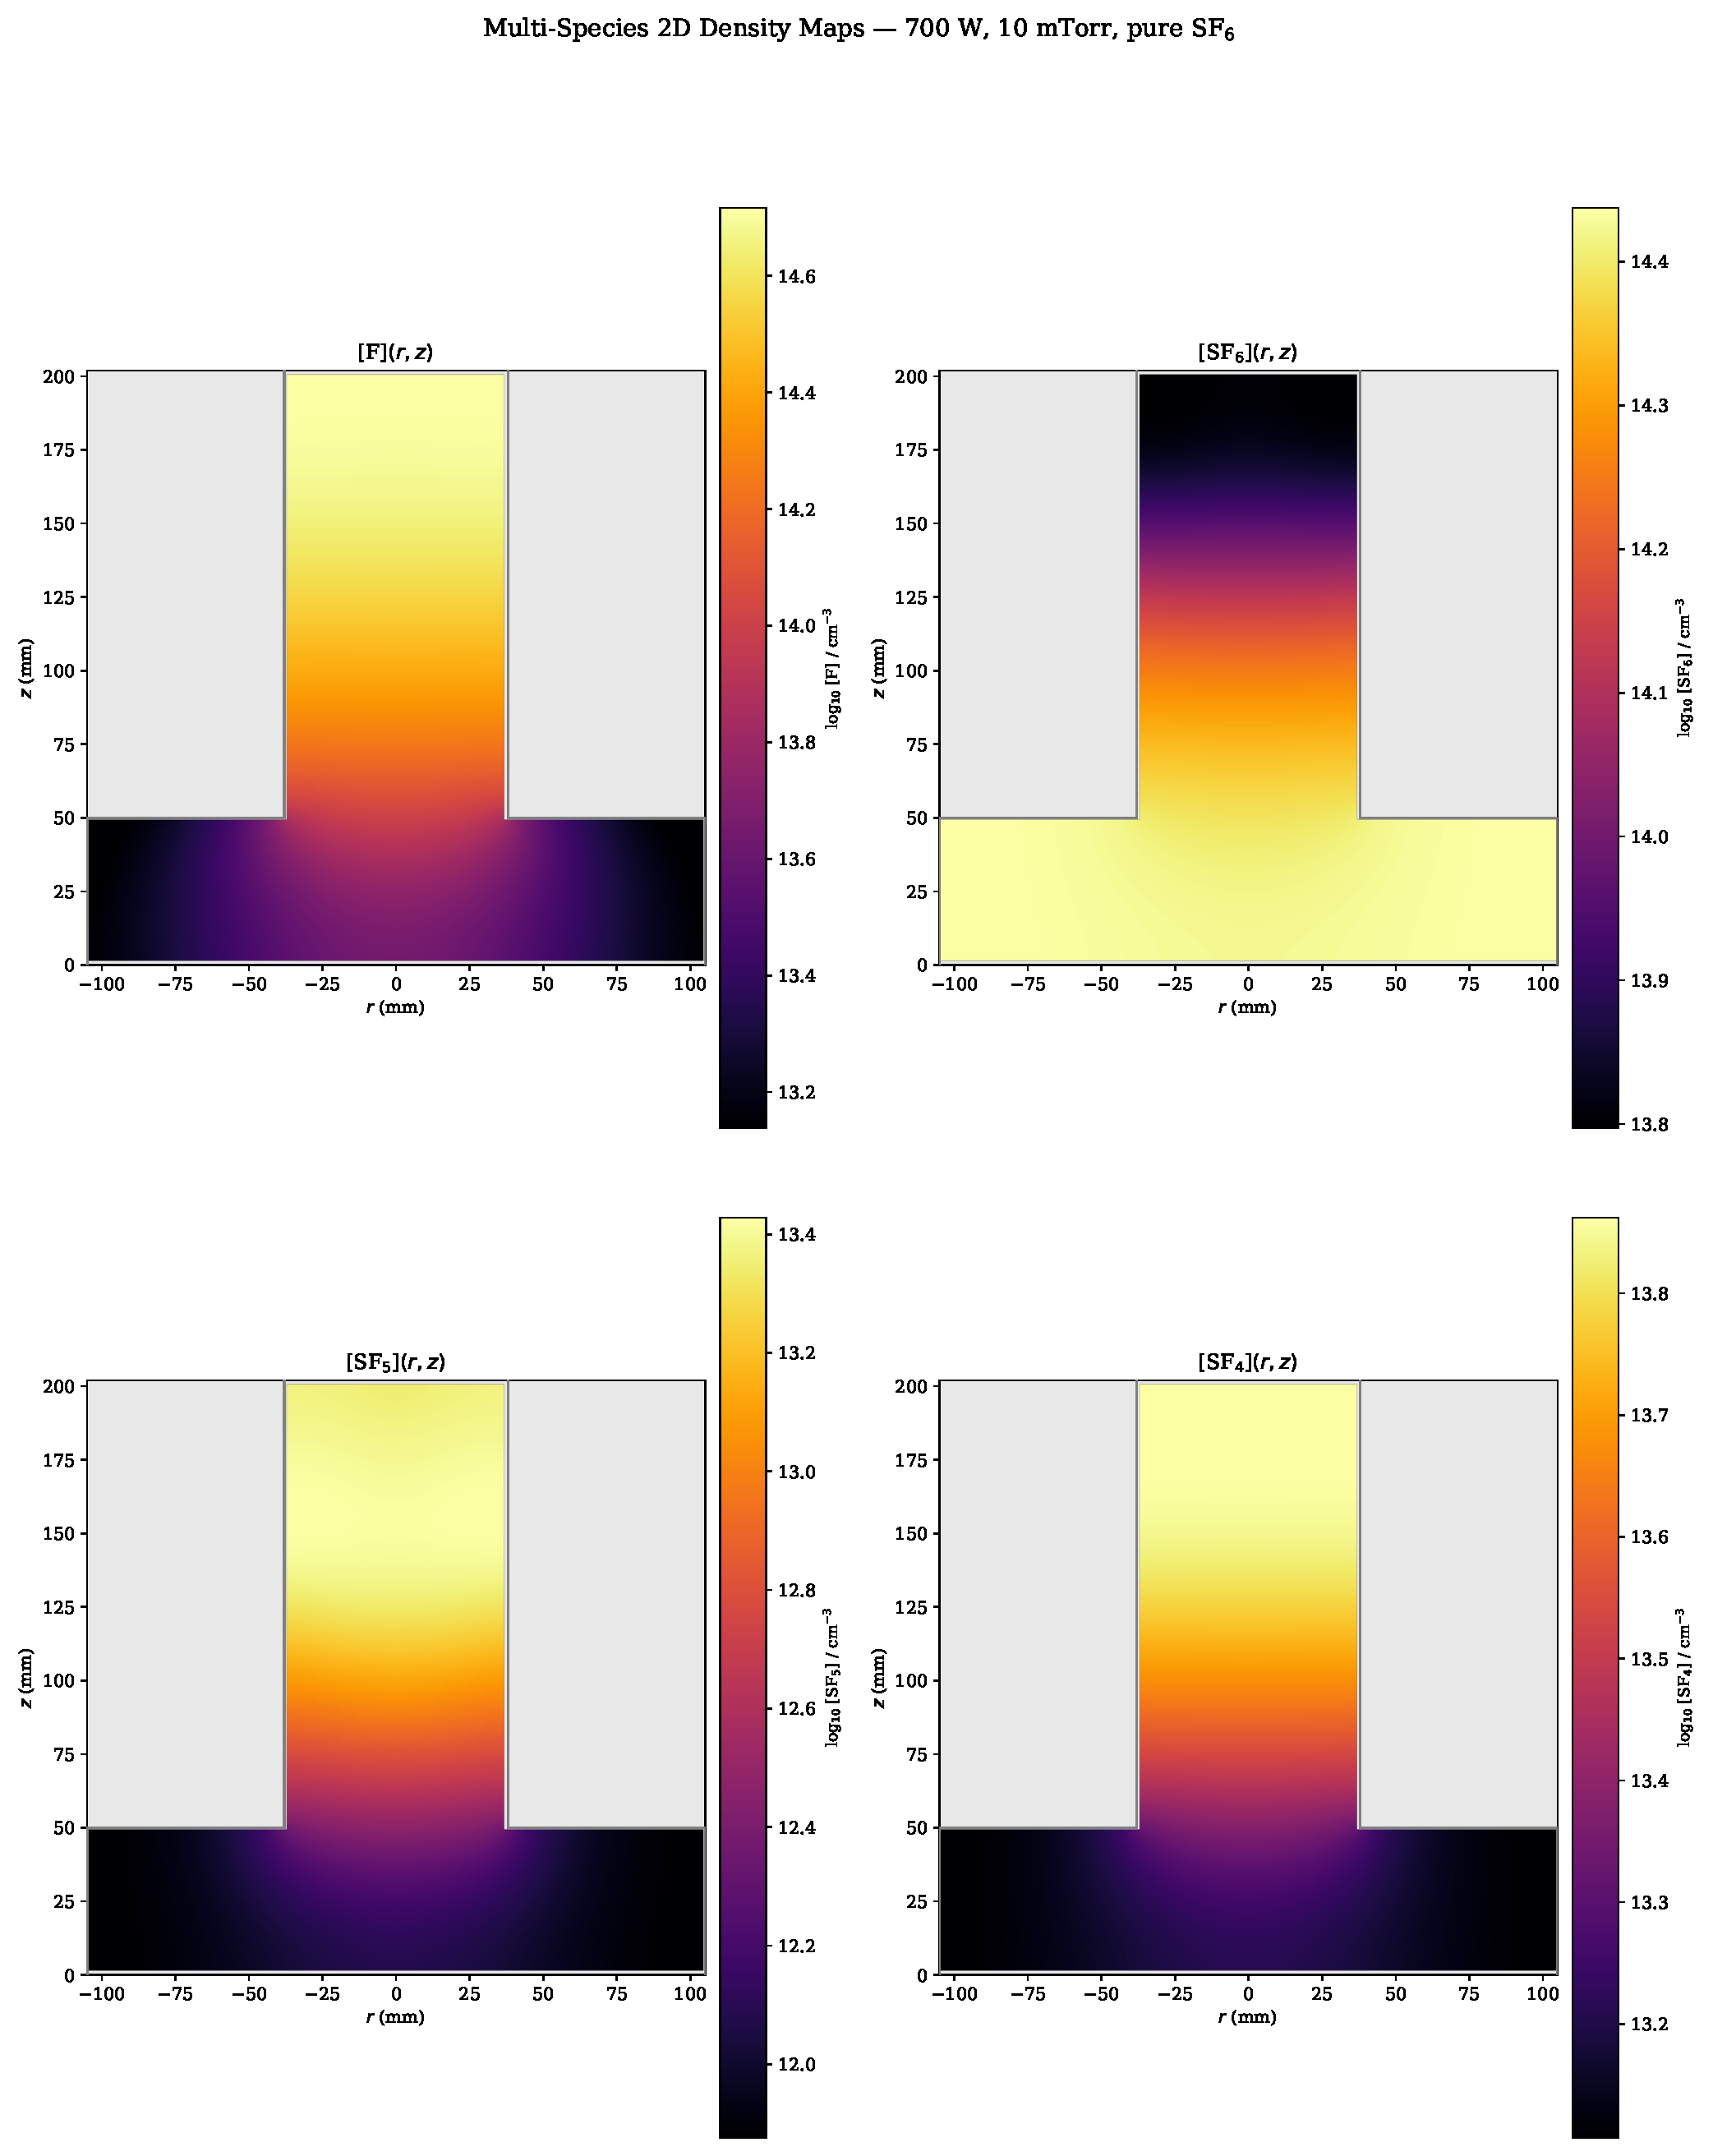
\includegraphics[width=0.95\textwidth]{fig_multispecies_contours}
  \caption{2D density maps of the four dominant neutral species on logarithmic scales (cm$^{-3}$).  F is concentrated in the ICP source; SF$_6$ is depleted in the source and replenished in the processing chamber; SF$_5$ and SF$_4$ are intermediate dissociation products with densities 1--2 orders of magnitude below the parent gas.}
  \label{fig:multispecies-contours}
\end{figure}

The deeper dissociation fragments (SF$_3$, SF$_2$, SF, S) show progressively lower densities consistent with the sequential electron-impact dissociation chain SF$_6 \to$ SF$_5 \to$ SF$_4 \to$ SF$_3 \to$ SF$_2 \to$ SF $\to$ S (Figure~\ref{fig:multispecies-contours-2}).

\begin{figure}[H]
  \centering
  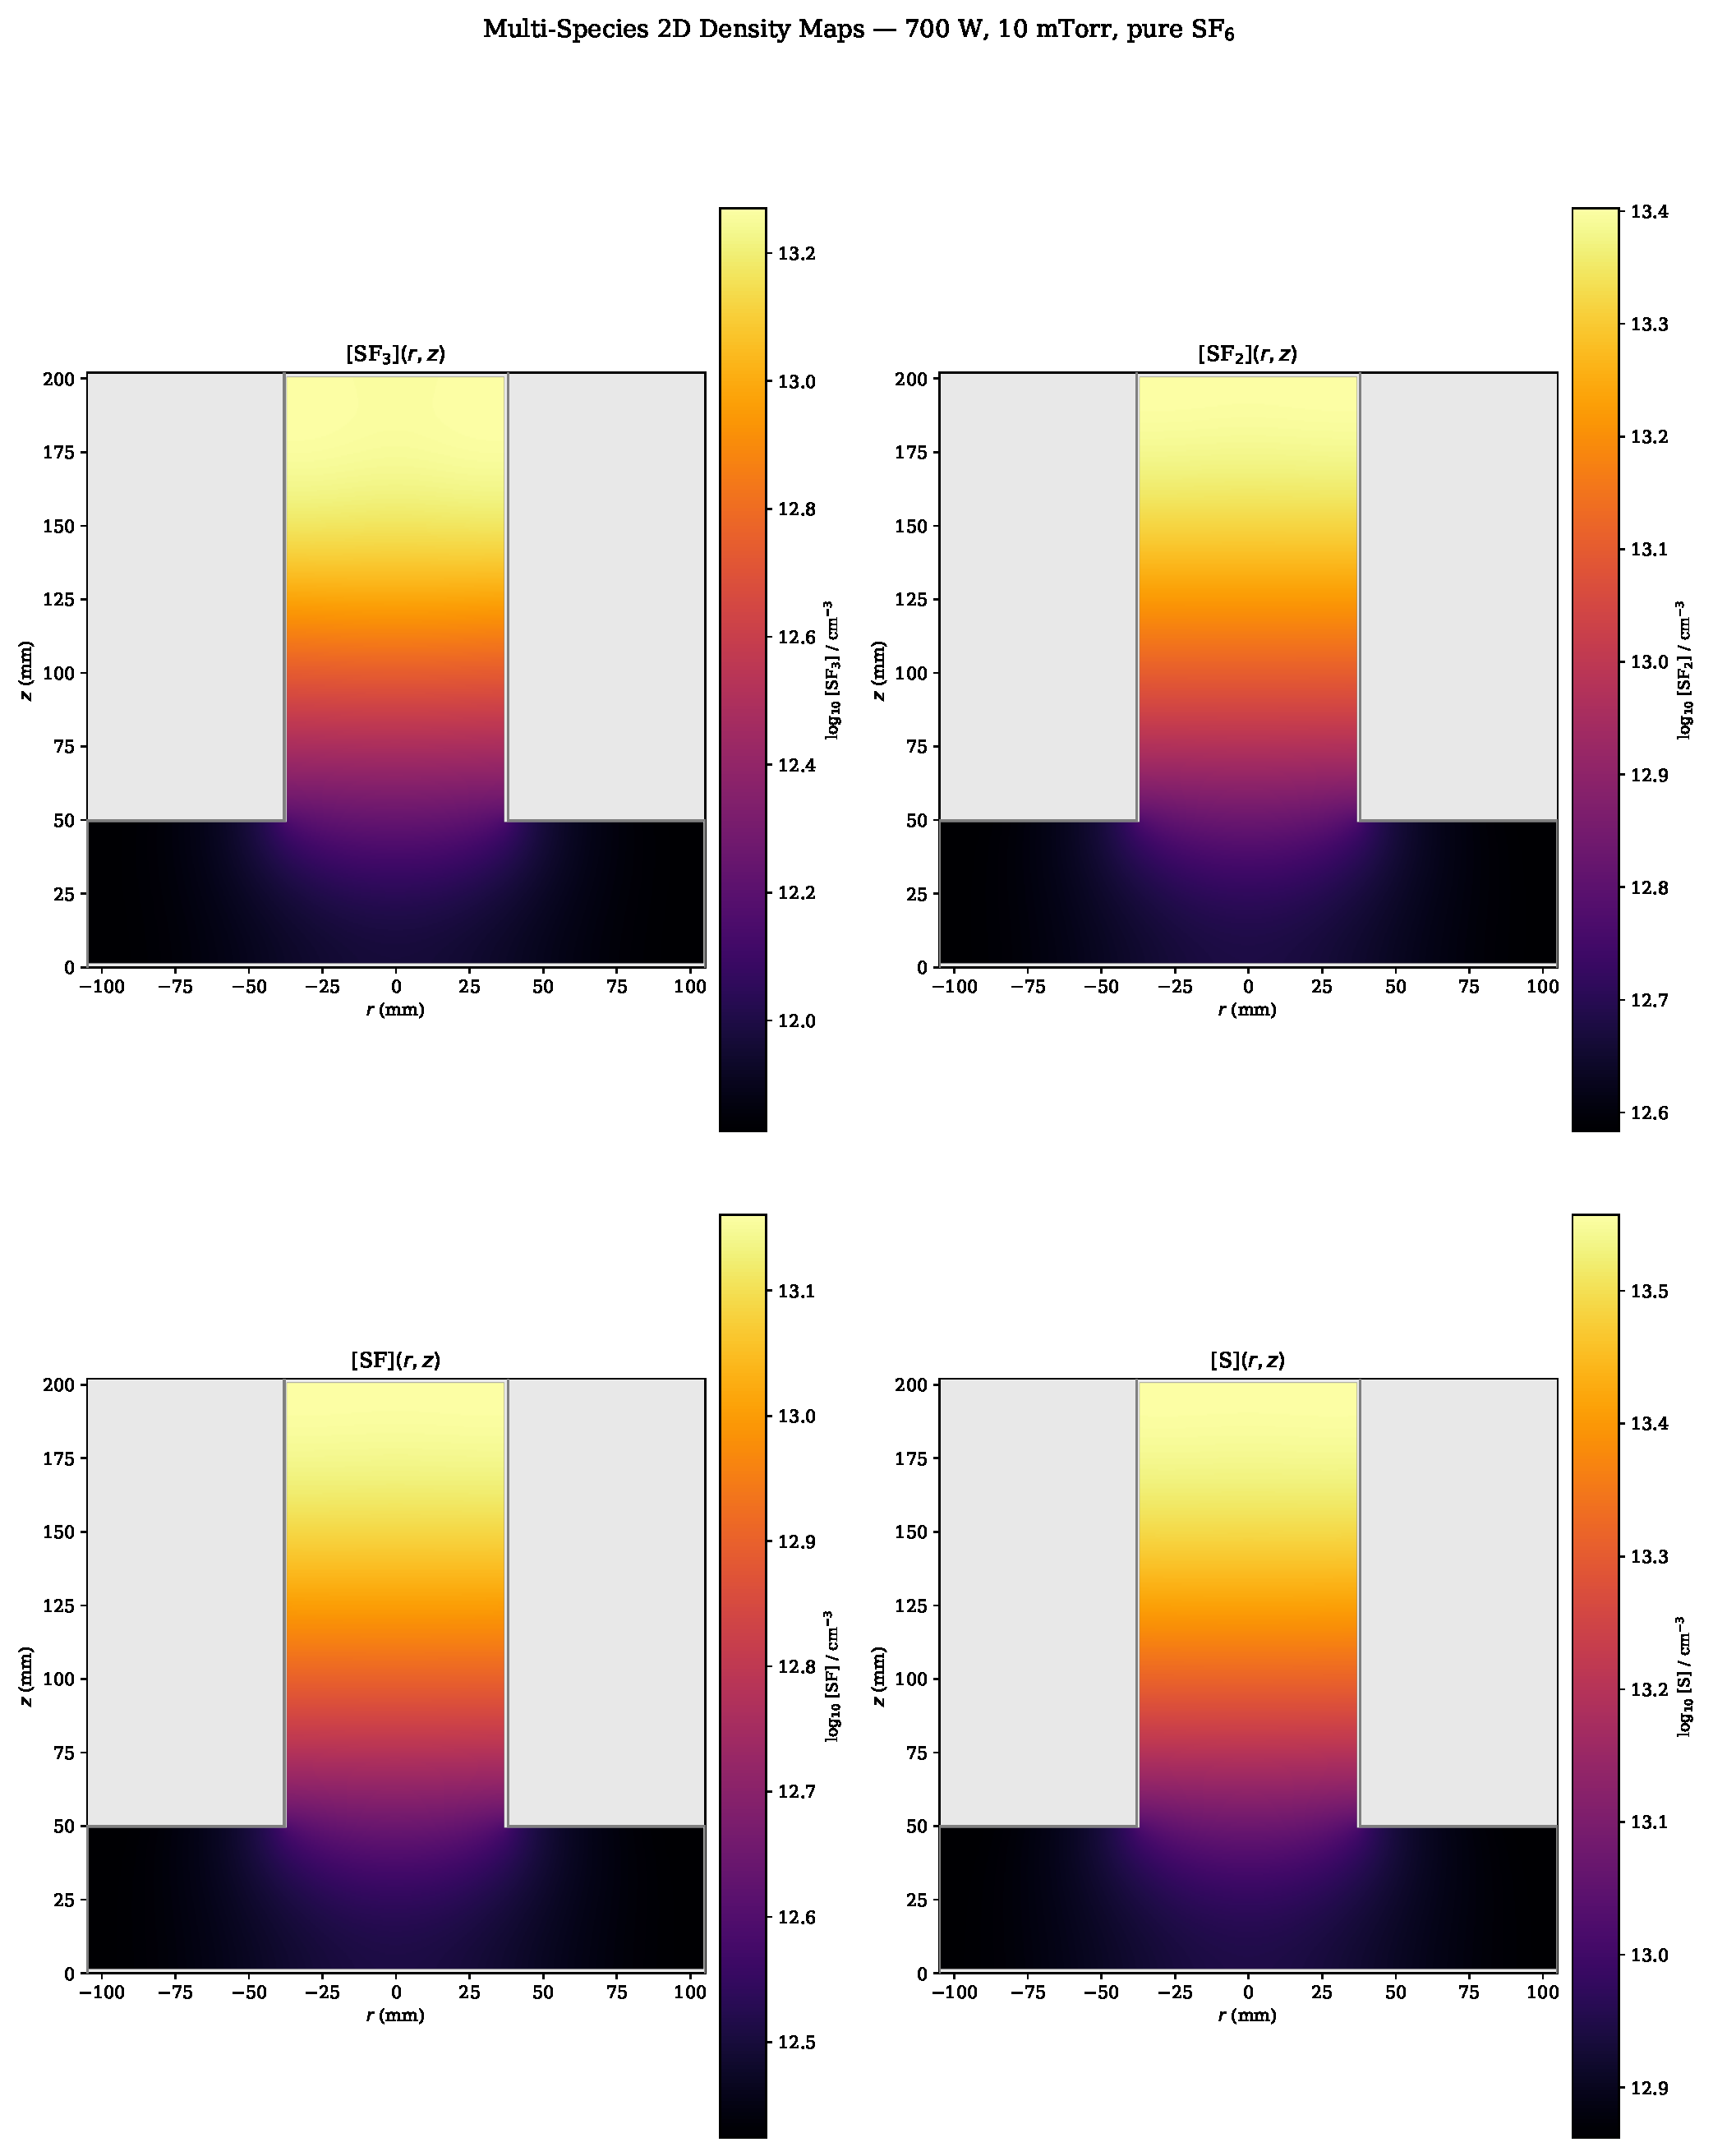
\includegraphics[width=0.95\textwidth]{fig_multispecies_contours_2}
  \caption{2D density maps of the deeper dissociation fragments SF$_3$, SF$_2$, SF, and S.  These species are produced by sequential electron-impact dissociation and are present at densities 2--4 orders of magnitude below SF$_6$.}
  \label{fig:multispecies-contours-2}
\end{figure}

\subsection{Charged Species}

The charged particle densities are computed from quasi-neutrality and the local attachment-recombination balance.  Figure~\ref{fig:charged} shows the electron density $n_e$, total positive ion density $n_+$, total negative ion density $n_-$, and the electronegativity parameter $\alpha = n_-/n_e$.

\begin{figure}[H]
  \centering
  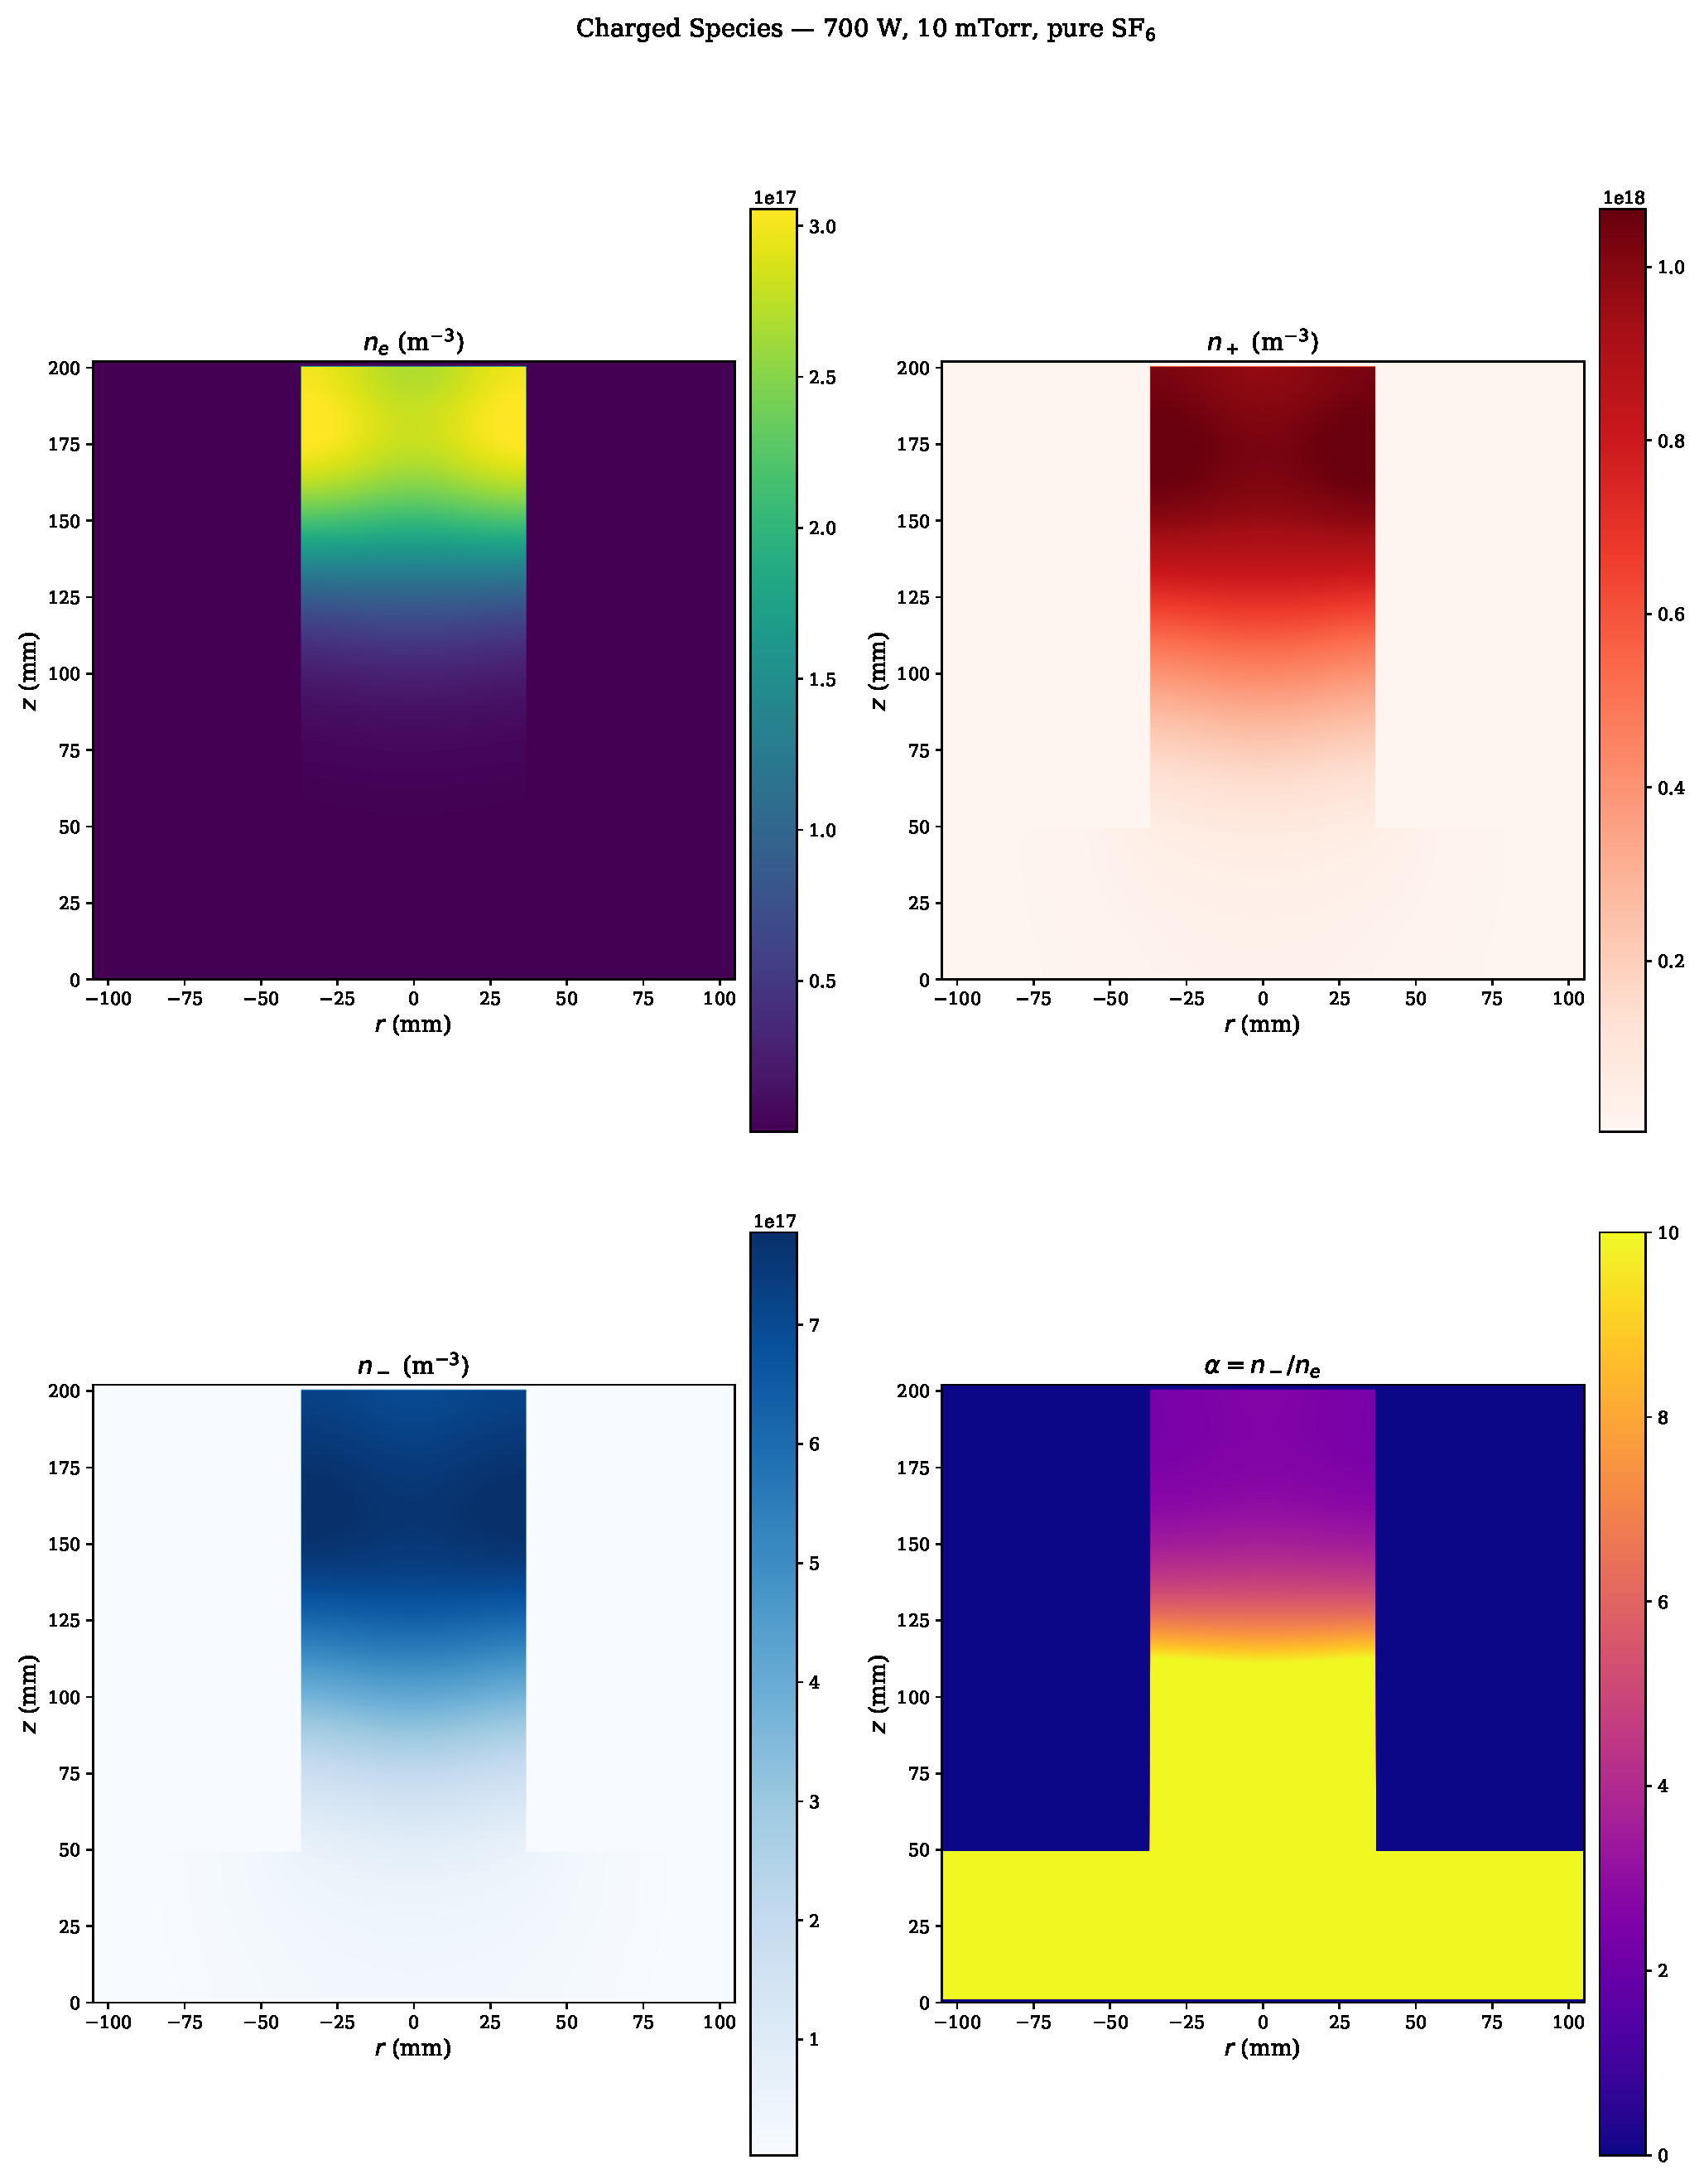
\includegraphics[width=0.95\textwidth]{fig_charged_species}
  \caption{Charged species distributions.  (a) Electron density $n_e$, peaked in the ICP source.  (b) Total positive ion density $n_+$.  (c) Total negative ion density $n_-$, dominated by SF$_6^-$ and F$^-$ from dissociative attachment.  (d) Electronegativity $\alpha = n_-/n_e$, reaching values of 3--10 in the processing chamber where attachment is strong relative to the low electron density.}
  \label{fig:charged}
\end{figure}

\subsection{Axial Species Profiles and Volume Averages}

Figure~\ref{fig:axial} presents the axial profiles of all nine neutral species along the reactor centreline ($r = 0$) and a bar chart of the volume-averaged densities.

\begin{figure}[H]
  \centering
  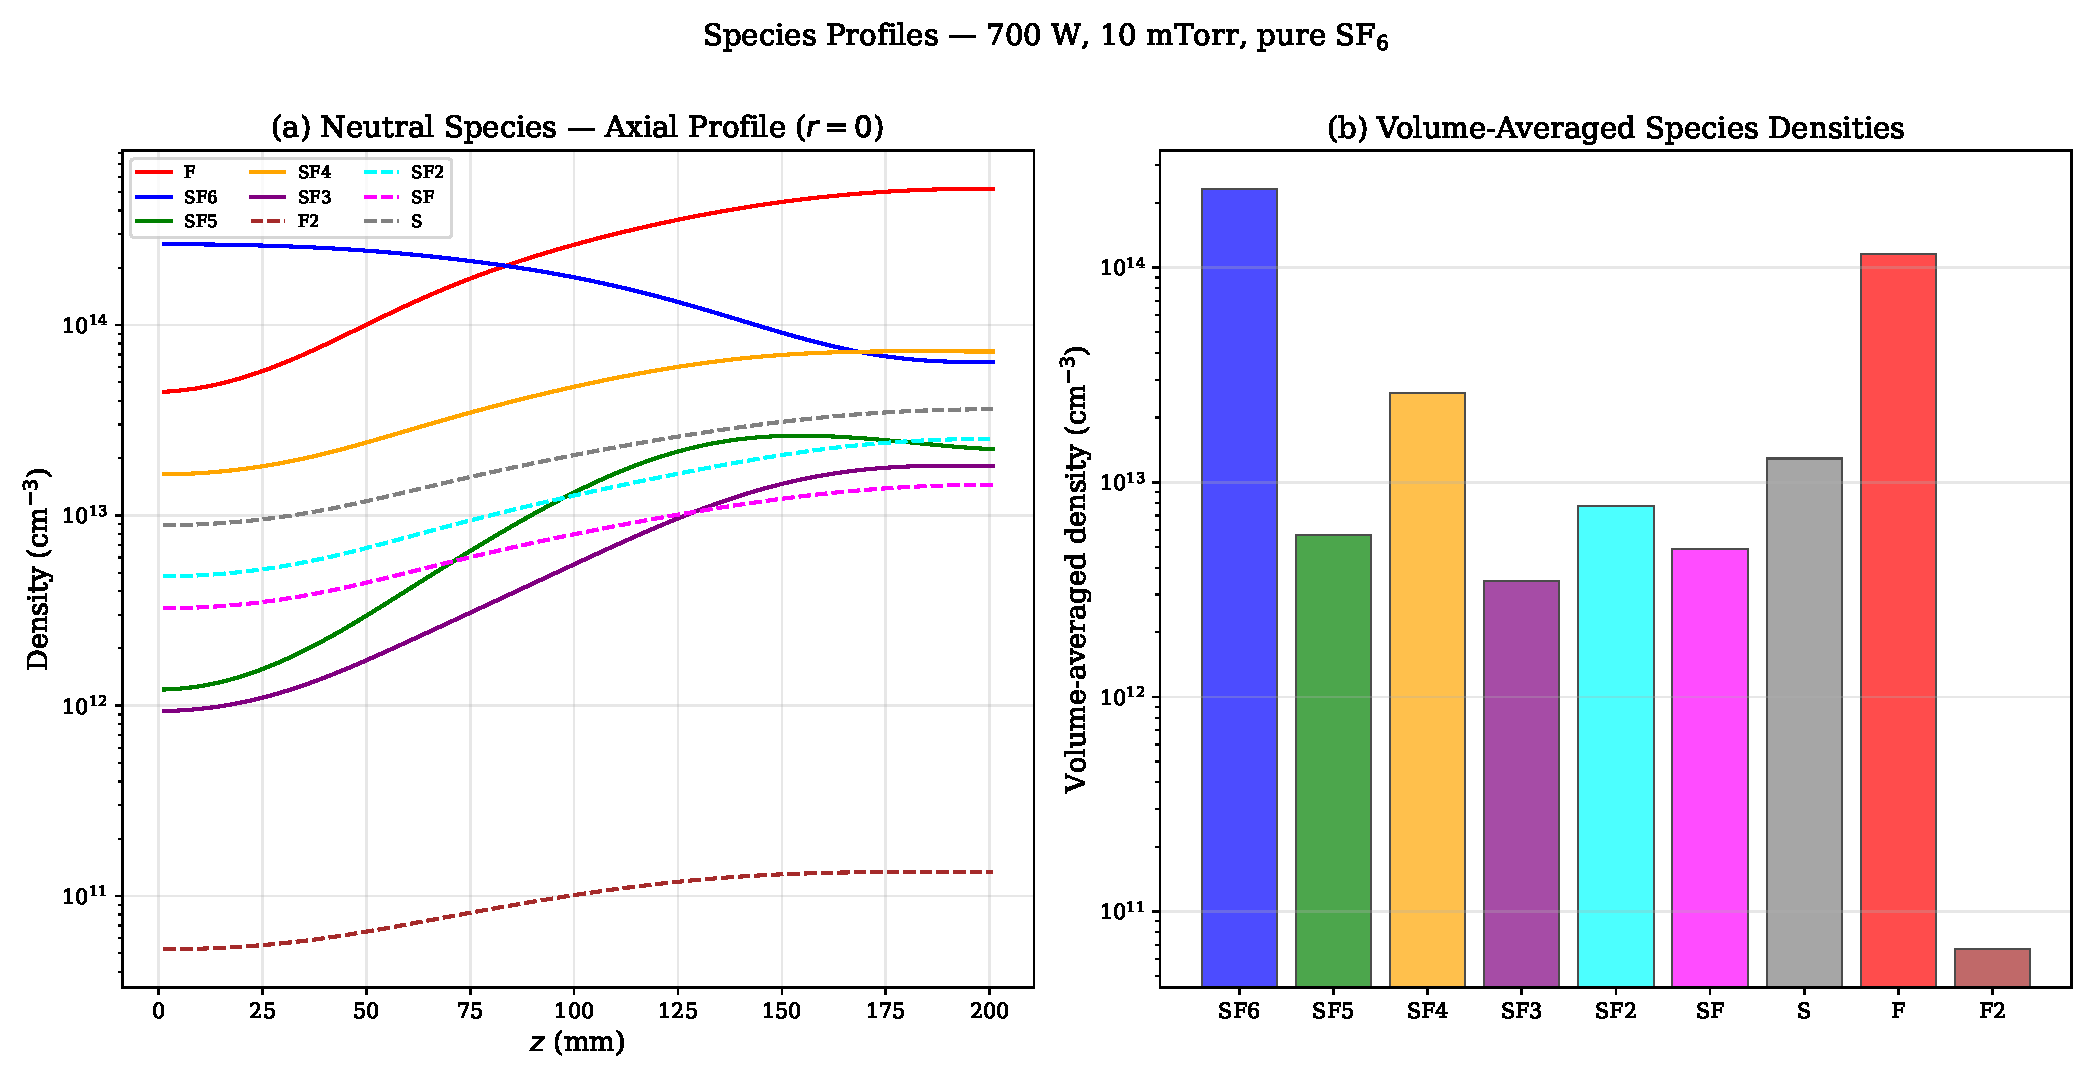
\includegraphics[width=0.95\textwidth]{fig_multispecies_axial}
  \caption{(a) Axial density profiles along the reactor centreline for all nine neutral species on a semi-logarithmic scale.  The sharp drop at $z \approx 50$~mm corresponds to the aperture transition between the ICP source and the processing chamber.  (b) Volume-averaged densities showing the species hierarchy: SF$_6 >$ F $>$ SF$_5 >$ SF$_4 >$ SF$_3$, consistent with the sequential dissociation cascade.}
  \label{fig:axial}
\end{figure}

\subsection{Wafer-Level Radical Profiles}

Figure~\ref{fig:wafer-profiles} presents the radial profiles of key quantities at the wafer surface, which are the most directly relevant to etch process control.

\begin{figure}[H]
  \centering
  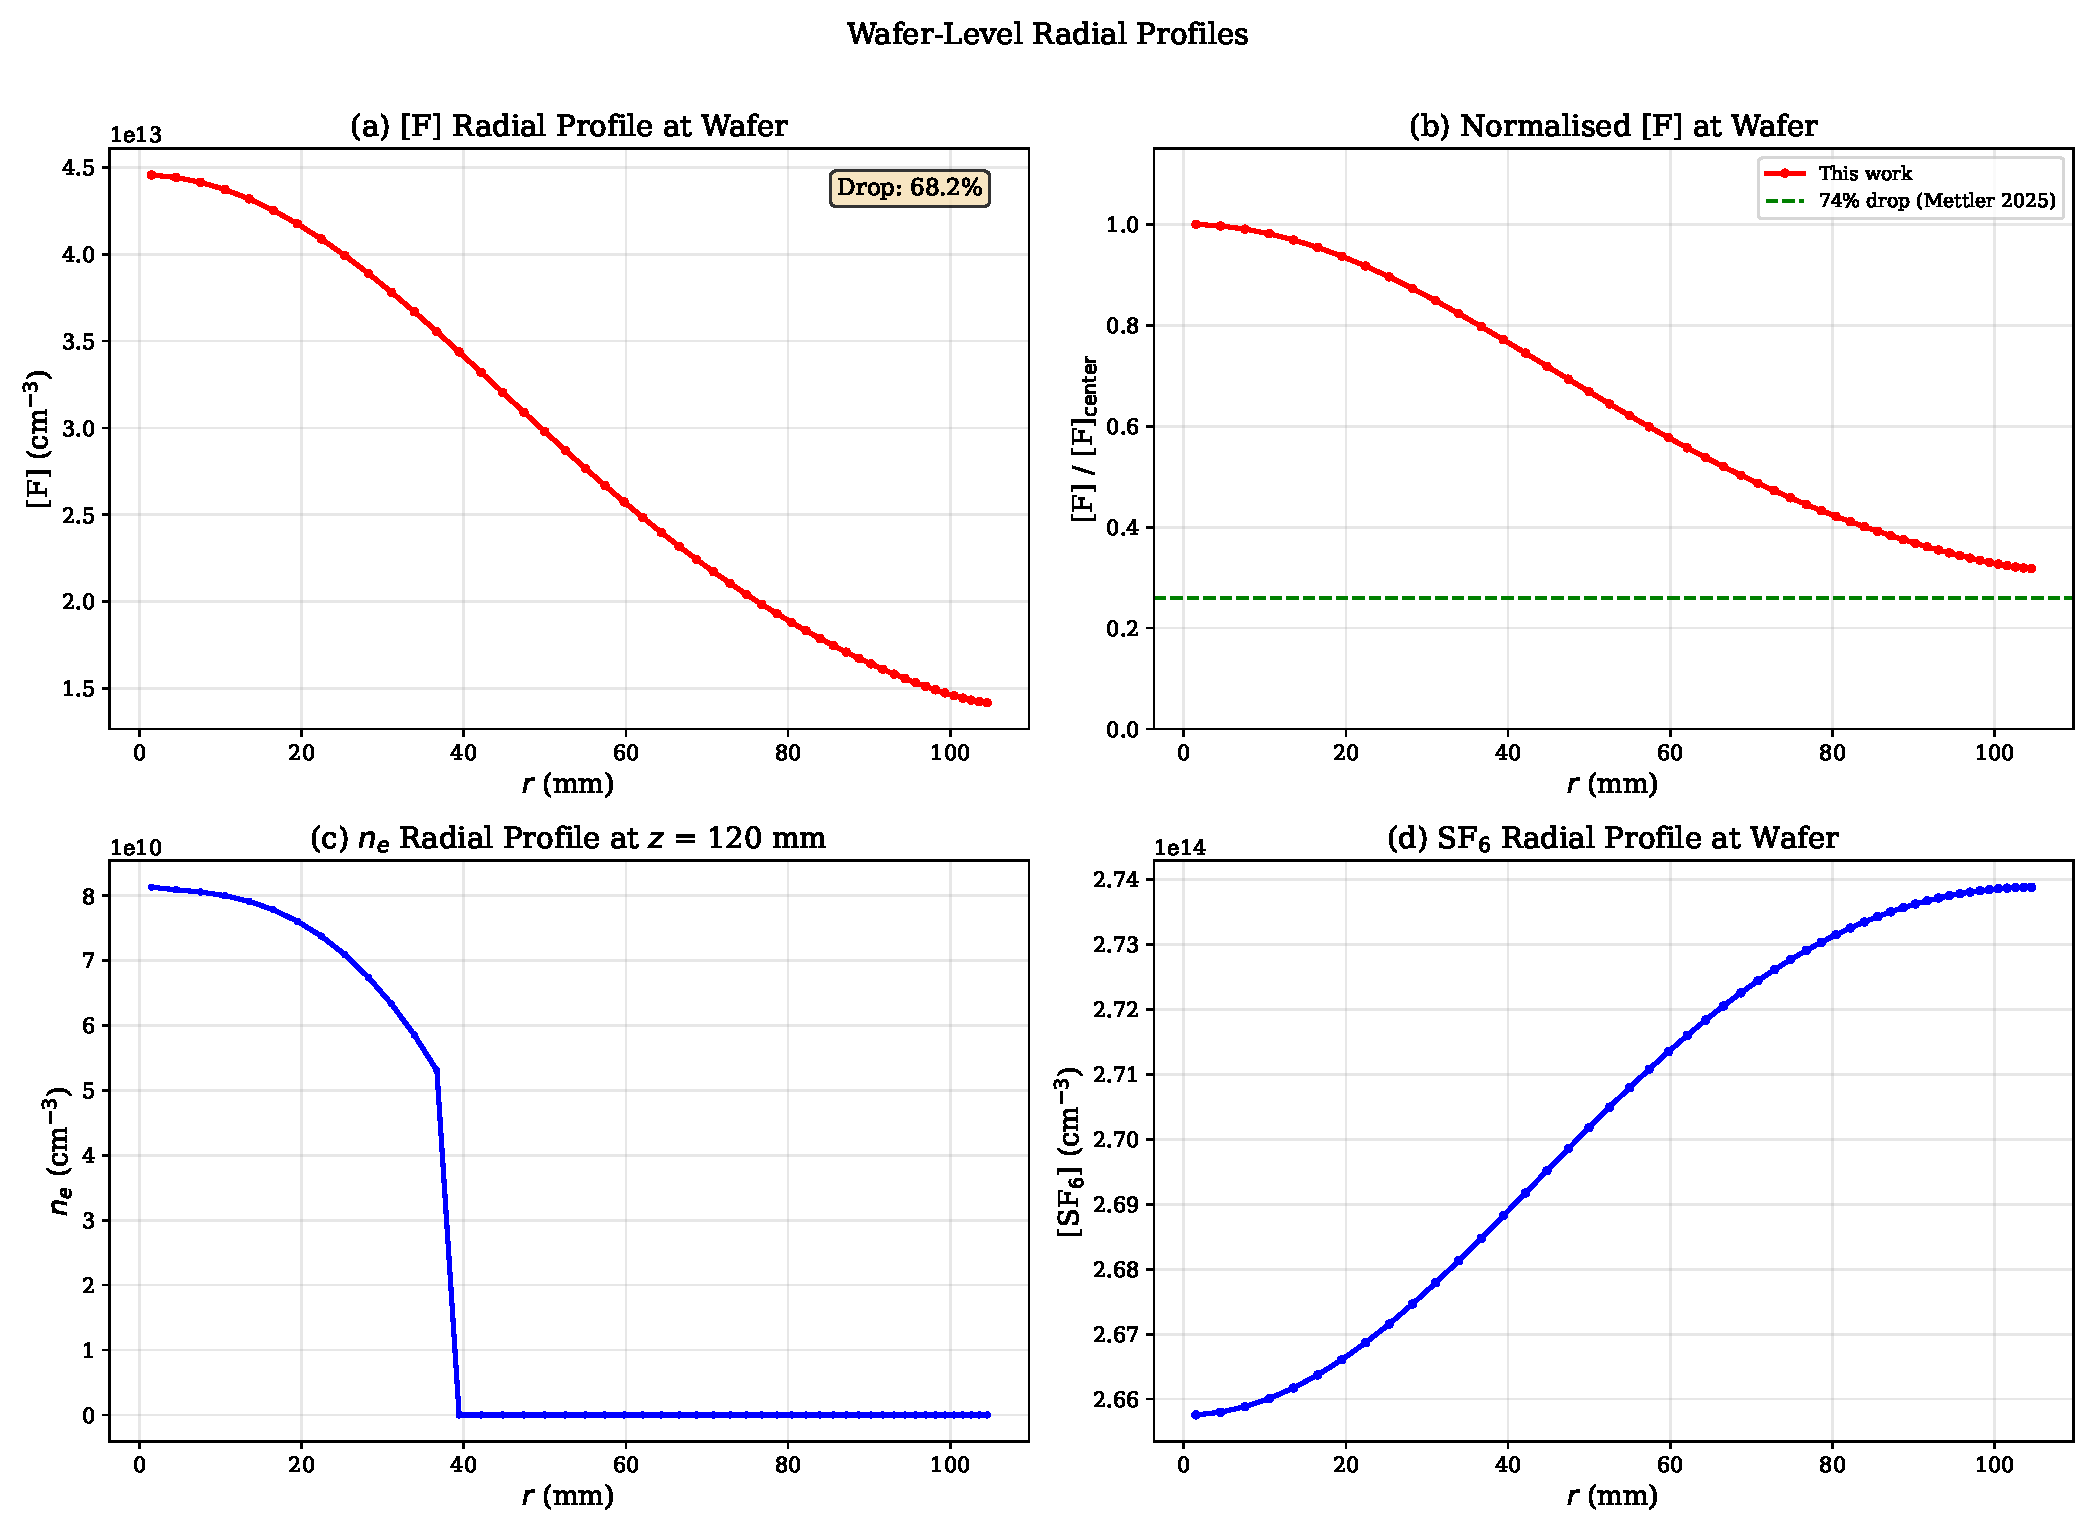
\includegraphics[width=0.75\textwidth]{fig_wafer_profiles}
  \caption{Radial profiles at the wafer surface ($z = 0$).  (a)~Absolute fluorine density showing the centre-to-edge drop of 68.2\%.  (b)~Normalised fluorine density with the Mettler 90\%-SF$_6$ bias-off reference level (dashed green, $74.5\,\%$ drop at \SI{1000}{\watt}, from Fig.~4.17)~\cite{Mettler2025}.  (c)~Electron density at the ICP midplane ($z = 139$~mm), peaked near $r \approx 20$~mm.  (d)~SF$_6$ density at the wafer, increasing toward the edge due to reduced dissociation.}
  \label{fig:wafer-profiles}
\end{figure}

The model prediction for the wafer-level [F] profile is compared directly with the Mettler radical-probe data in Figure~\ref{fig:radial-F-mettler}.  The coupled framework reproduces the experimental five-point normalised radial profile within $\pm 10$\,\% over the inner half of the wafer ($r < 4$~cm), while over-predicting by 15--27\,\% at the outer points ($r = 6$--$8$~cm).  In the prior revision this residual was attributed to the omitted electronegative ambipolar correction; the present revision implements that correction (\S\ref{sec:electronegative-ambipolar}) and finds that at the self-consistent $\alpha \approx 0.02$ the correction factor is only $\sim 1.02$, so it does not close the residual.  The remaining gap is now attributed primarily to the composition-insensitive $\gamma_\mathrm{Al} = 0.18$ calibration, which is a Phase-3 scope item.  A direct absolute-[F] benchmark at Mettler's actual operating conditions (\SI{1000}{\watt}, 30\% and 90\% SF$_6$) is given in Section~\ref{sec:mettler-fig417-direct}.

\begin{figure}[H]
  \centering
  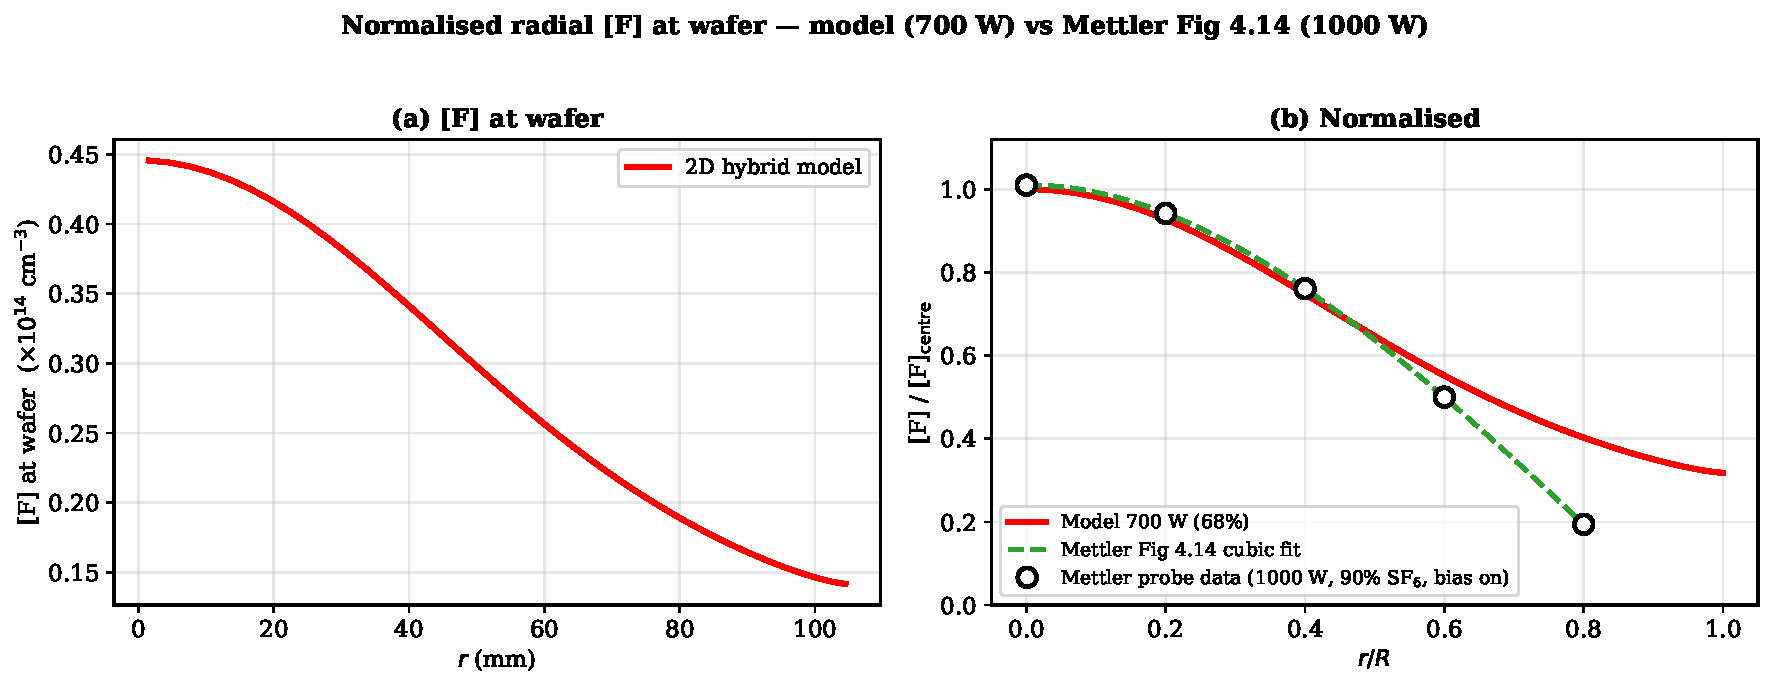
\includegraphics[width=0.85\textwidth]{fig_radial_F_wafer_mettler}
  \caption{Normalised radial [F] profile at the wafer.  (a)~Absolute model prediction at the present-work design-baseline (\SI{700}{\watt}, \SI{10}{\milli\torr}, pure SF$_6$).  (b)~Normalised profile overlaid with the five-point Mettler Fig.~4.17 data (open circles, 90\% SF$_6$ bias-off composition) and the Fig.~4.14 cubic fit (dashed green, $y(r) = 1.01032 - 0.01847r^2 + 7.139\times 10^{-4}r^3$).  Mettler Fig.~4.14 was recorded at 70~sccm SF$_6$ / 30~sccm Ar with \SI{200}{\watt} rf bias --- a different composition and bias from the design-baseline shown in panel (a).  The design-baseline model matches the inner half ($r < 4$~cm) within $\pm 10$\,\% but over-predicts the outer half by 15--27\,\%; the 6--8~pp under-shoot in the centre-to-edge drop \emph{is not} attributable to the electronegative ambipolar correction (which has only a $\sim 2\,\%$ effect at the self-consistent $\alpha \approx 0.02$; see \S\ref{sec:electronegative-ambipolar}) but rather to the composition-insensitive $\gamma_\mathrm{Al}$ calibration.  An apples-to-apples benchmark at Mettler's exact operating conditions is given in Section~\ref{sec:mettler-fig417-direct}.}
  \label{fig:radial-F-mettler}
\end{figure}

The axial structure of the fluorine density from the ICP source to the wafer is dominated by the 2\,mm aperture transition.  Figure~\ref{fig:axial-F} plots the axial [F] along the reactor centreline.

\begin{figure}[H]
  \centering
  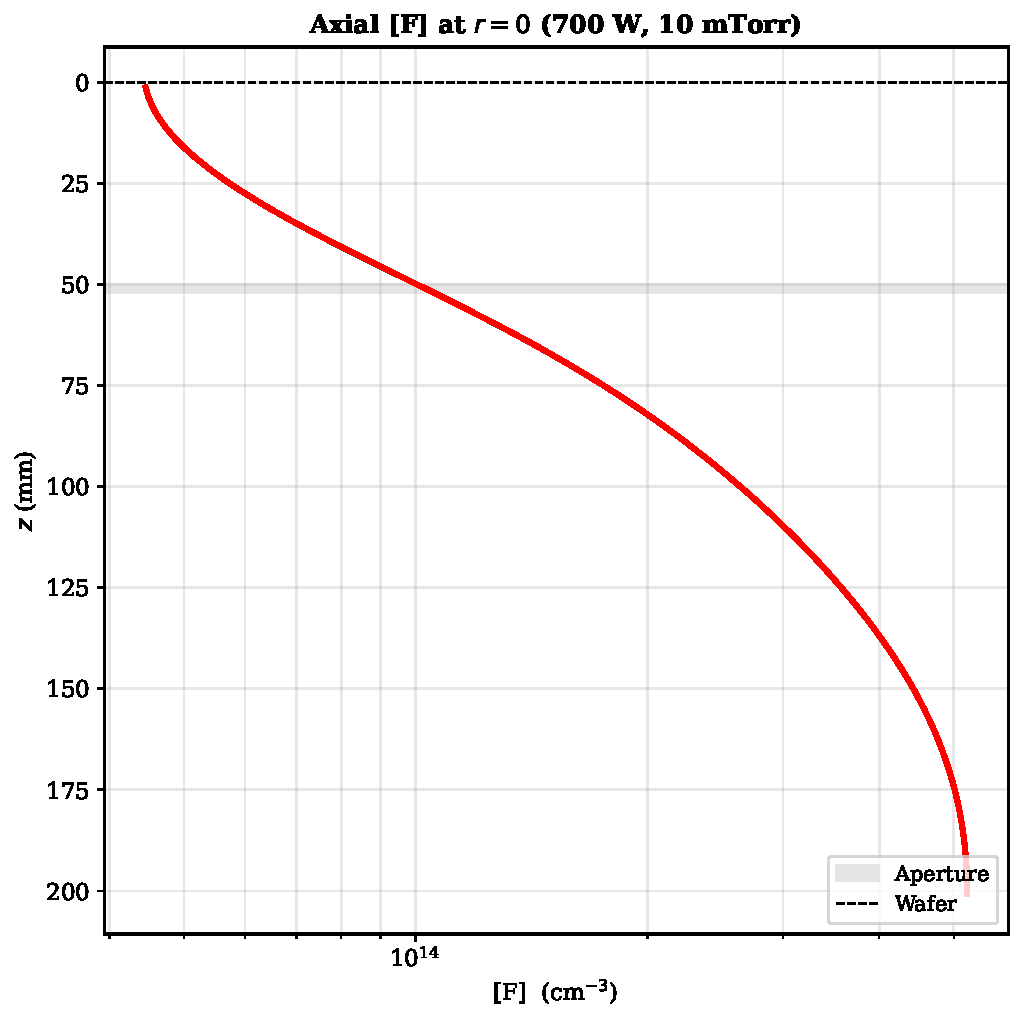
\includegraphics[width=0.55\textwidth]{fig_axial_F_profile}
  \caption{Axial [F] profile along the reactor centreline at $r = 0$ (700\,W, 10\,mTorr).  The grey shaded band marks the 2\,mm aperture at $z = 50$\,mm; the dashed line marks the wafer at $z = 0$.  The sharp gradient across and below the aperture demonstrates that the bulk of the centre-to-edge [F] drop accumulates during transport from the ICP source into the processing chamber, not purely across the narrow aperture itself.}
  \label{fig:axial-F}
\end{figure}

The full 9-species radial profiles at the wafer surface are shown in Figure~\ref{fig:all-species-radial}.  Each species exhibits a characteristic radial dependence: the dissociation products (F, SF$_5$, SF$_4$, SF$_3$) decrease from centre to edge (following the electron density gradient), while the parent gas SF$_6$ increases toward the edge (reflecting reduced dissociation in the periphery).

\begin{figure}[H]
  \centering
  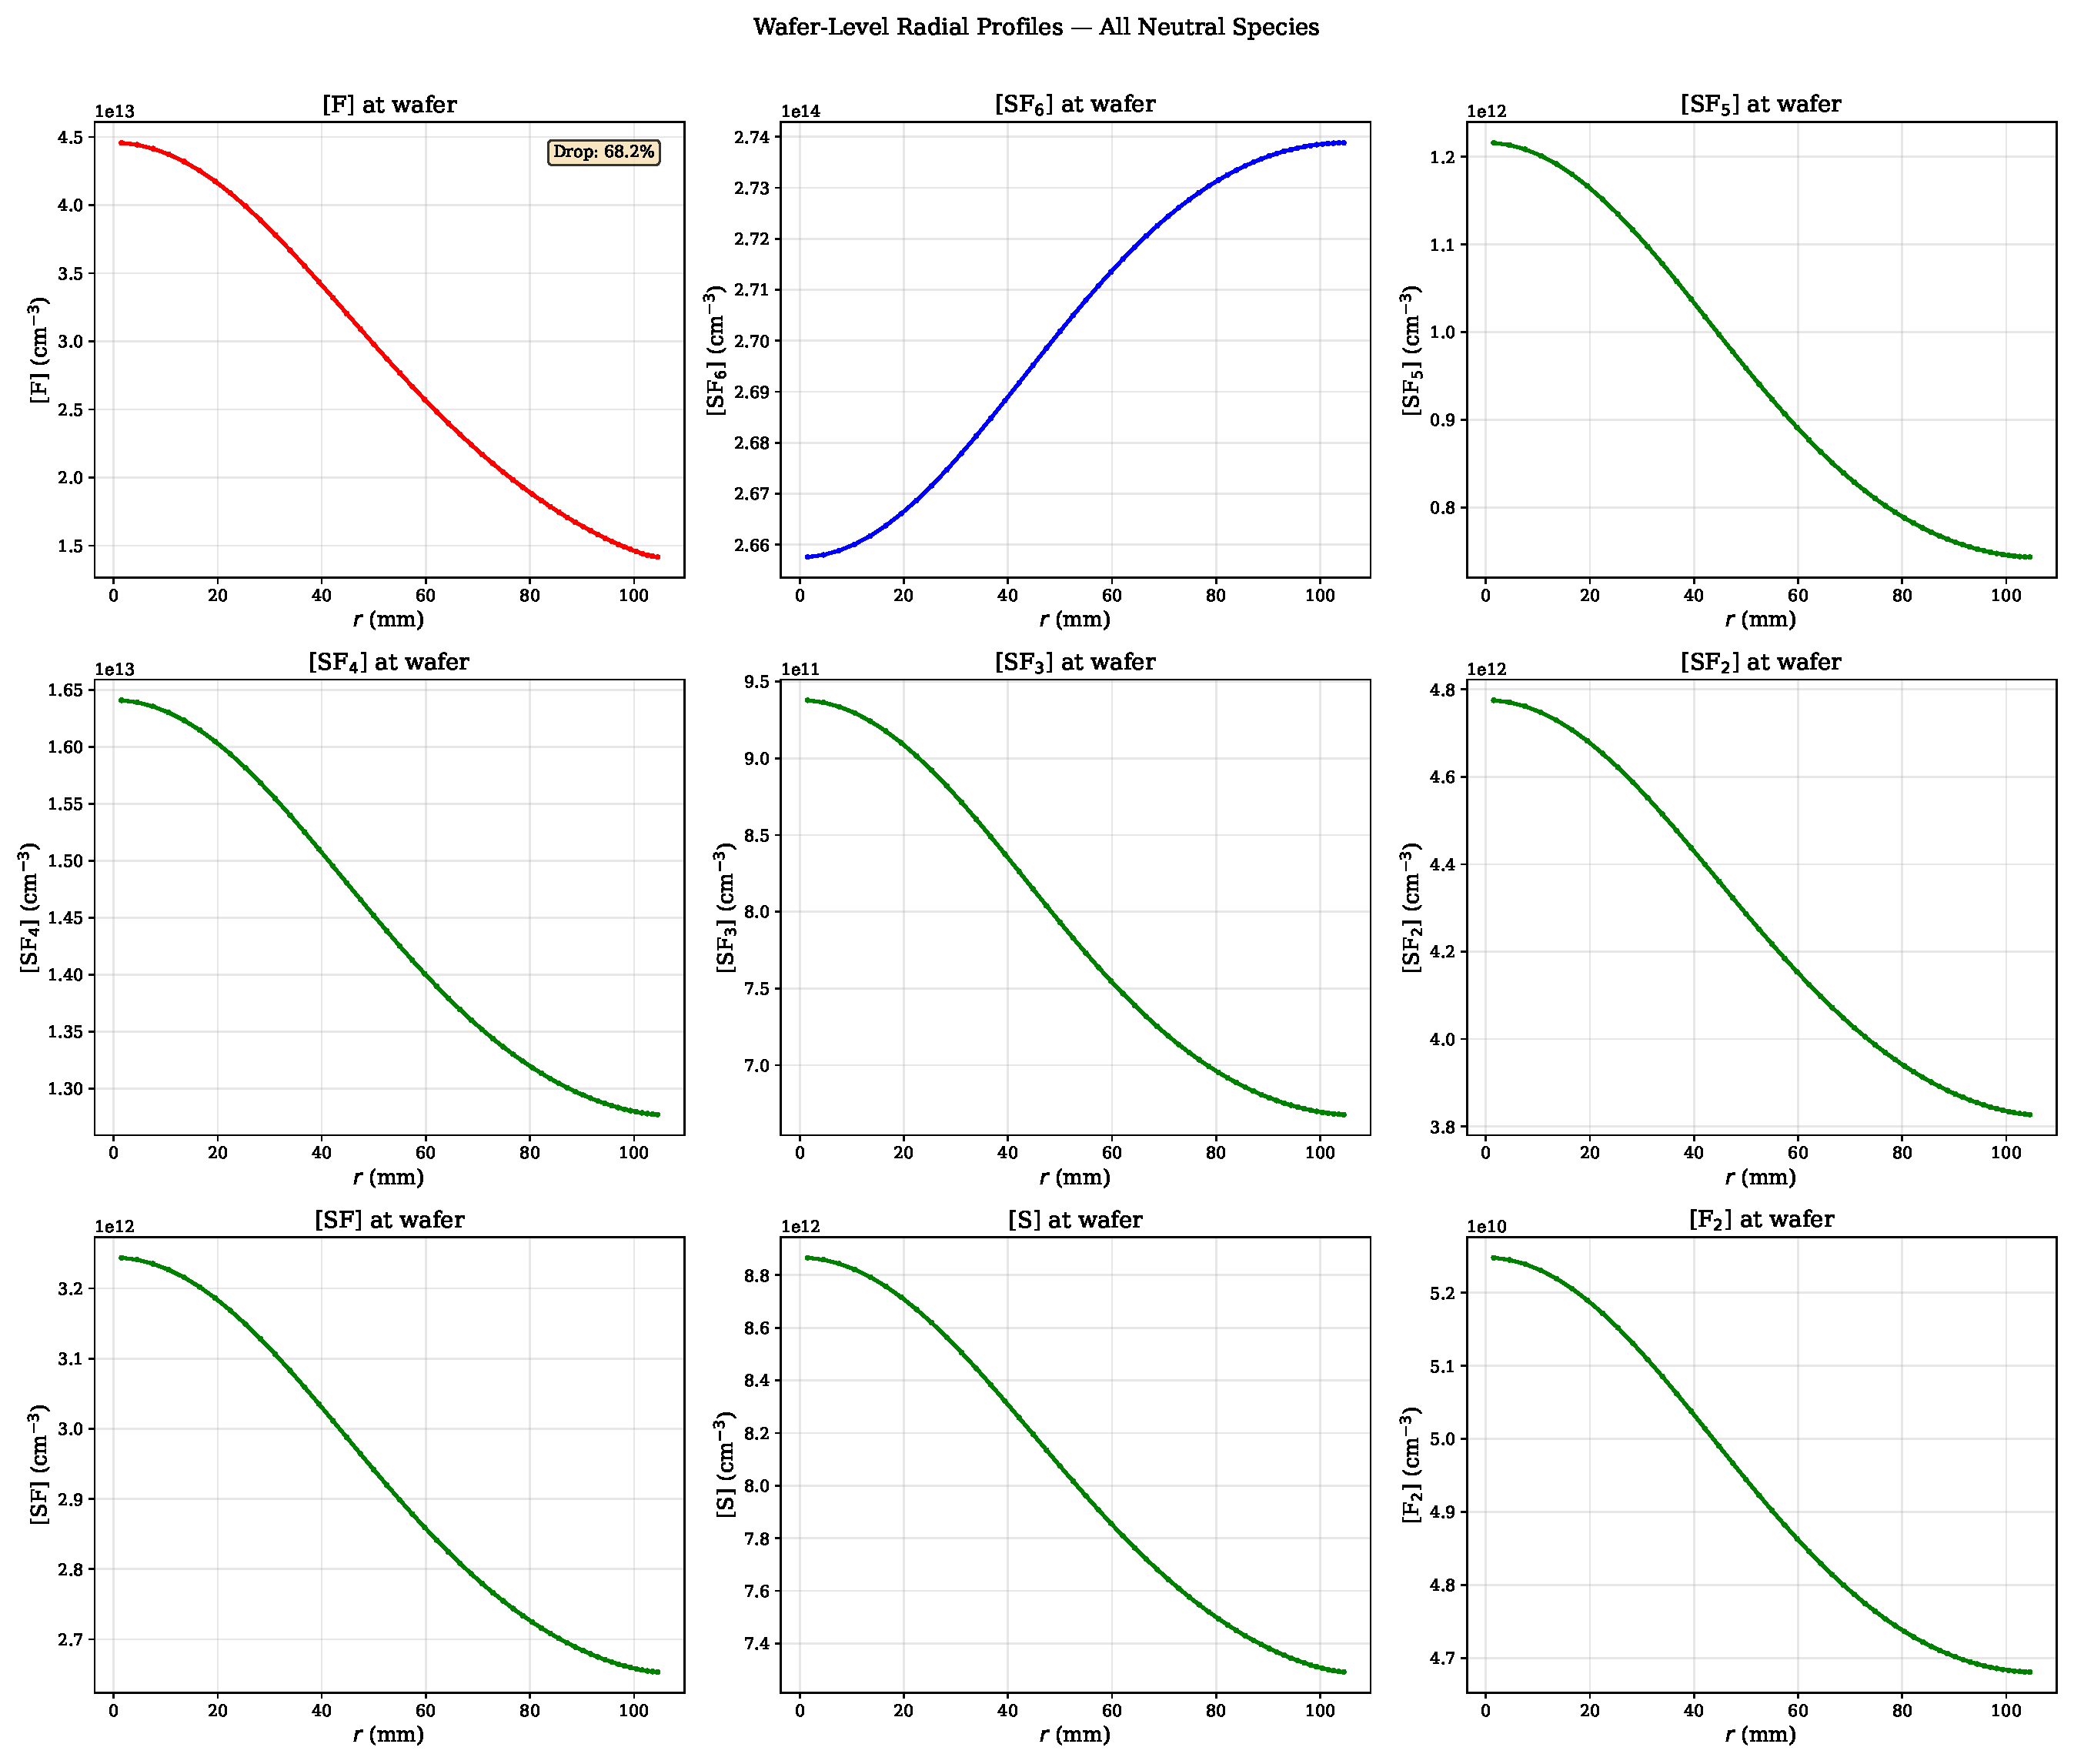
\includegraphics[width=0.95\textwidth]{fig_multispecies_radial}
  \caption{Wafer-level radial profiles of all nine neutral species.  The dissociation products (F, SF$_5$, SF$_4$, etc.) decrease from centre to edge, while the parent gas SF$_6$ and molecular fluorine F$_2$ increase toward the edge.  The contrasting behaviour reflects the spatial distribution of the electron-impact dissociation source.}
  \label{fig:all-species-radial}
\end{figure}

\subsection{Consolidated Species Overlay}

Figure~\ref{fig:species-overlay} presents all nine neutral species on a single logarithmic plot at the wafer surface, clearly showing the three-decade density hierarchy from the parent gas SF$_6$ ($\sim 3 \times 10^{14}$~cm$^{-3}$) down to atomic sulphur ($\sim 5 \times 10^{11}$~cm$^{-3}$).

\begin{figure}[H]
  \centering
  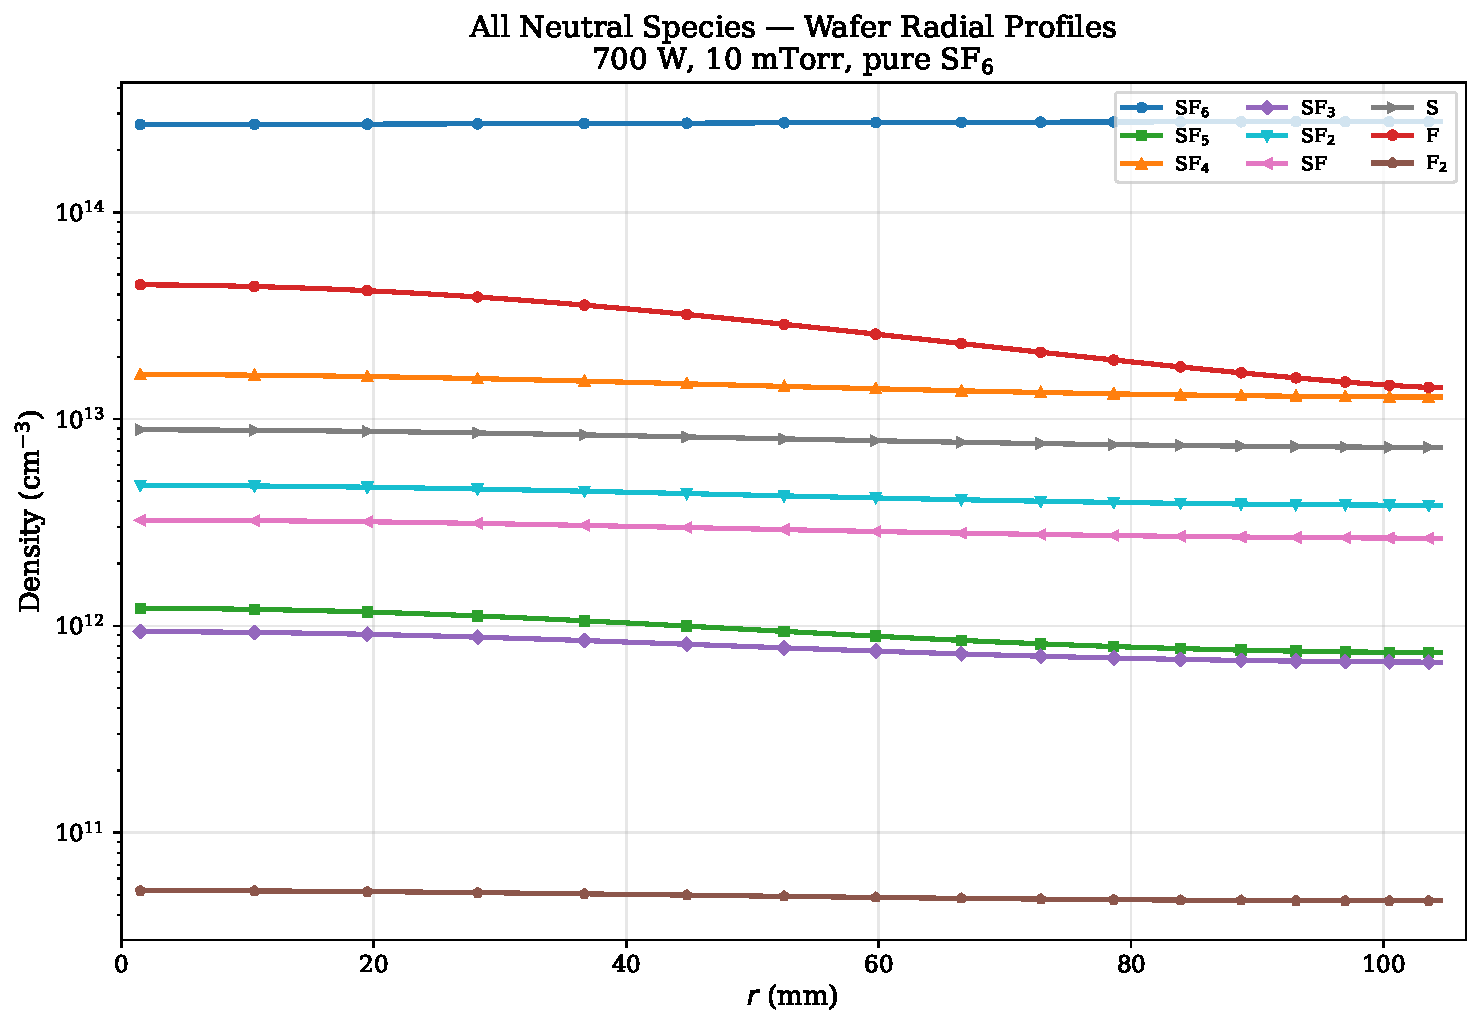
\includegraphics[width=0.85\textwidth]{fig_all_species_radial_overlay}
  \caption{Consolidated overlay of all nine neutral species densities at the wafer surface on a semi-logarithmic scale.  The species hierarchy (SF$_6 >$ F $>$ SF$_5 >$ SF$_4 >$ F$_2 >$ SF$_3 >$ SF$_2 >$ SF $>$ S) is consistent with the sequential electron-impact dissociation chain modulated by Troe-corrected recombination.}
  \label{fig:species-overlay}
\end{figure}

\subsection{Regional Comparison and Dissociation Chain}

Figure~\ref{fig:bar-chart} compares the volume-averaged species densities between the ICP source region (where dissociation is active) and the processing chamber (where only diffusion and wall chemistry operate).

\begin{figure}[H]
  \centering
  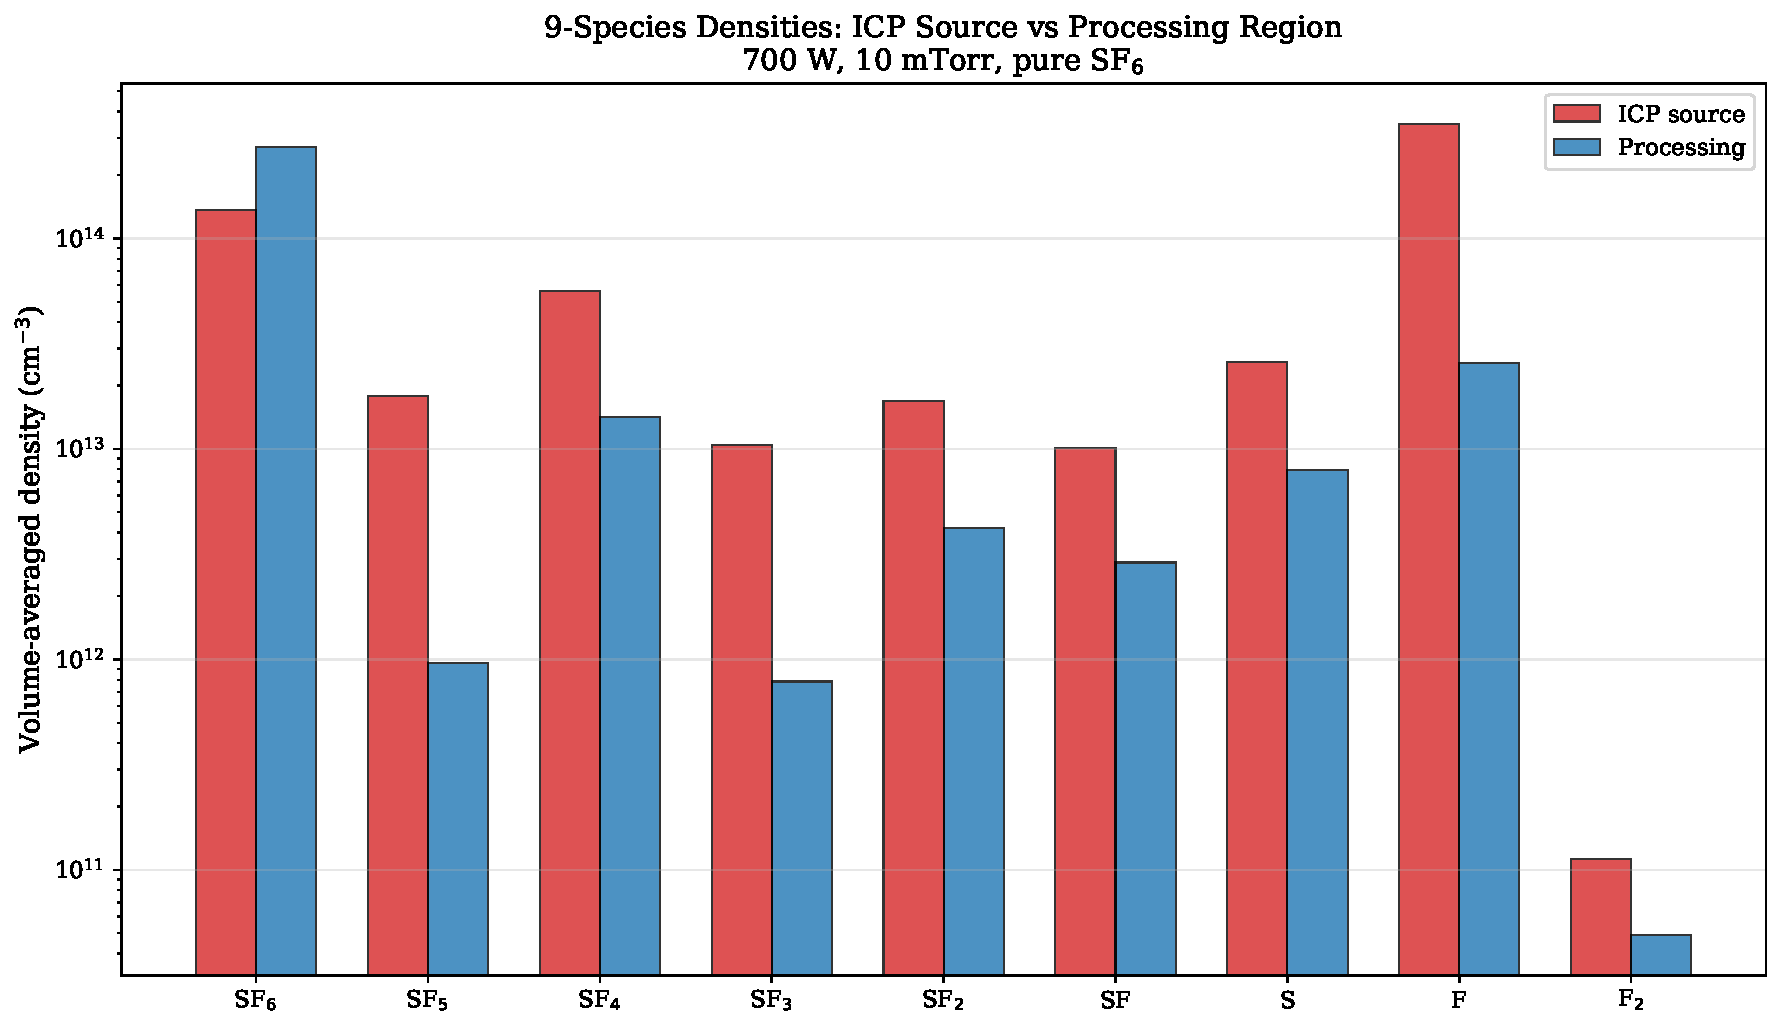
\includegraphics[width=0.85\textwidth]{fig_species_bar_chart}
  \caption{Grouped bar chart comparing volume-averaged densities of all nine neutral species in the ICP source region (red) versus the processing chamber (blue).  The parent gas SF$_6$ is more abundant in the processing region (less dissociation), while the dissociation fragments are more concentrated in the ICP source where electron-impact reactions are vigorous.}
  \label{fig:bar-chart}
\end{figure}

The sequential dissociation chain from SF$_6$ to atomic sulphur is shown in Figure~\ref{fig:chain}, which traces the average density at each step of the fragmentation pathway for both reactor regions.

\begin{figure}[H]
  \centering
  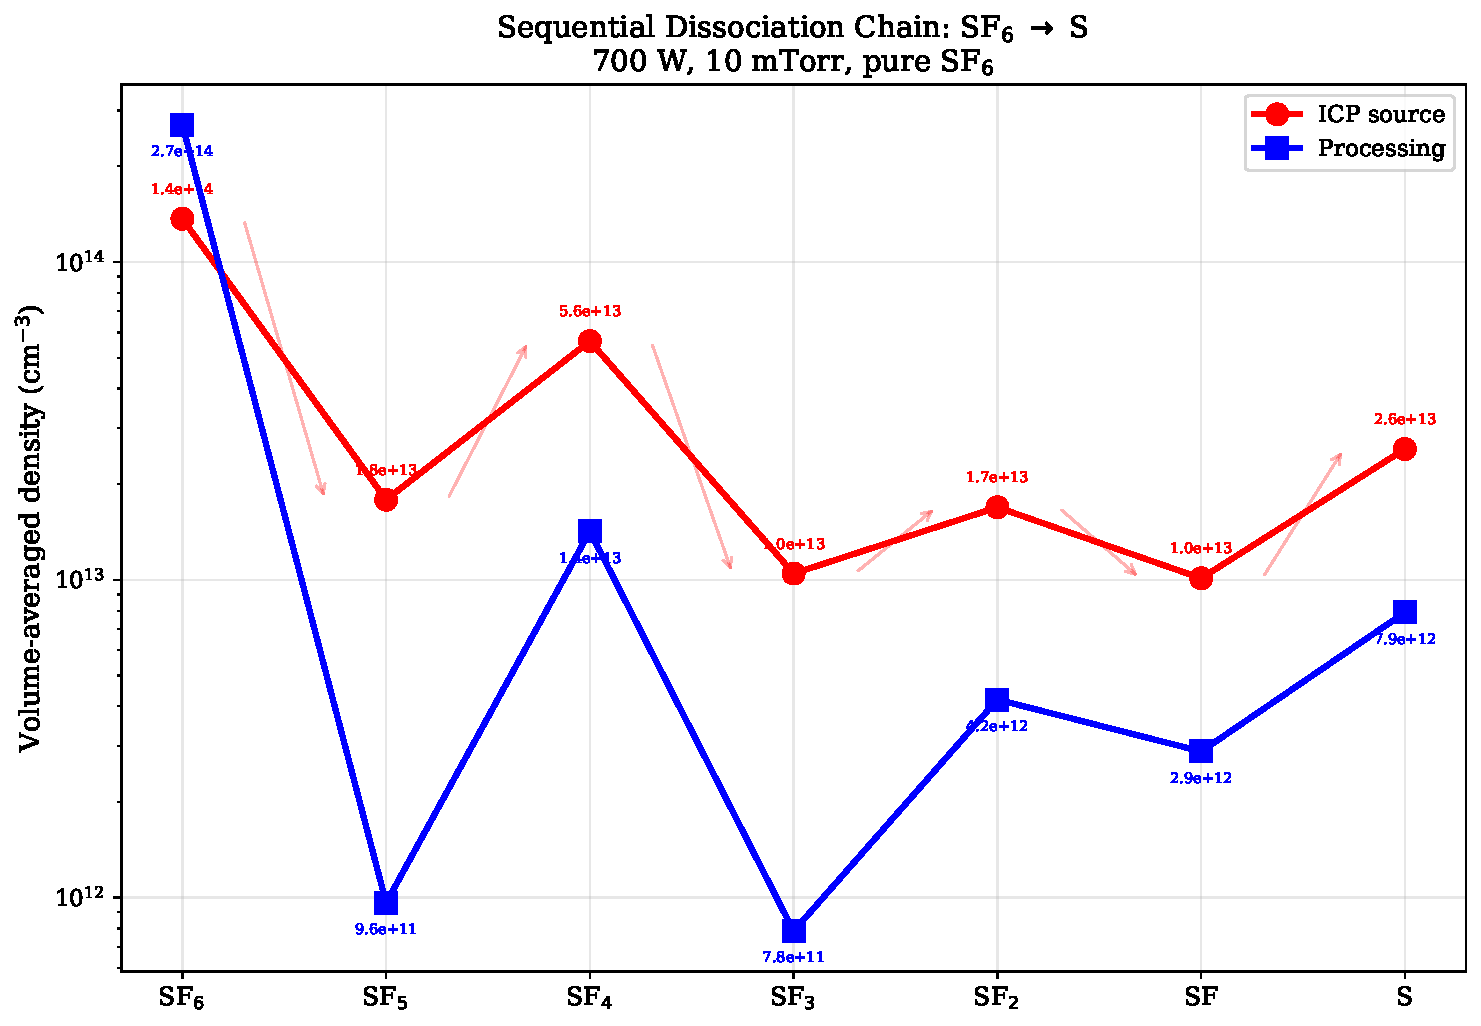
\includegraphics[width=0.85\textwidth]{fig_dissociation_chain}
  \caption{Sequential dissociation chain: SF$_6 \to$ SF$_5 \to$ SF$_4 \to$ SF$_3 \to$ SF$_2 \to$ SF $\to$ S.  The ICP source (red) and processing chamber (blue) volume-averaged densities are shown at each fragmentation step.  The non-monotonic behaviour of SF$_4$ (higher than SF$_5$ in the ICP) reflects competing production from SF$_6$ dissociation and loss from further fragmentation.}
  \label{fig:chain}
\end{figure}

Panel~(b) is the primary validation diagnostic.  The normalised F profile $n_\mathrm{F}(r)/n_\mathrm{F}(0)$ decreases monotonically from 1 at the centre to $\sim 0.22$ at $r = 105$~mm.  The experimental $74.5\,\%$ drop level for 90\,\%~SF$_6$ bias-off (corresponding to $n_\mathrm{F}/n_\mathrm{F}(0) = 0.255$, from Fig.~4.17~\cite{Mettler2025}) is shown as a dashed green line; the model prediction crosses this level at $r \approx 80$~mm and reaches a somewhat lower value at the full chamber radius.  Mettler's 30\,\%~SF$_6$ bias-off branch has a shallower drop ($67.2\,\%$, $n_\mathrm{F}/n_\mathrm{F}(0) = 0.328$) that the fixed-$\gamma_\mathrm{Al}$ model does not reproduce.

Panel~(c) shows the electron density profile at the ICP source midplane.  The peak at $r \approx 20$~mm---rather than on the axis---reflects the finite radial extent of the ionization source (driven by the skin-depth power deposition) modulated by ambipolar diffusion and wall loss.  This off-axis peak is a genuine prediction of the self-consistent model and differs from the on-axis maximum of the prescribed Bessel--cosine eigenmode used in the initial formulation.

\subsection{Summary Overview}

\begin{figure}[H]
  \centering
  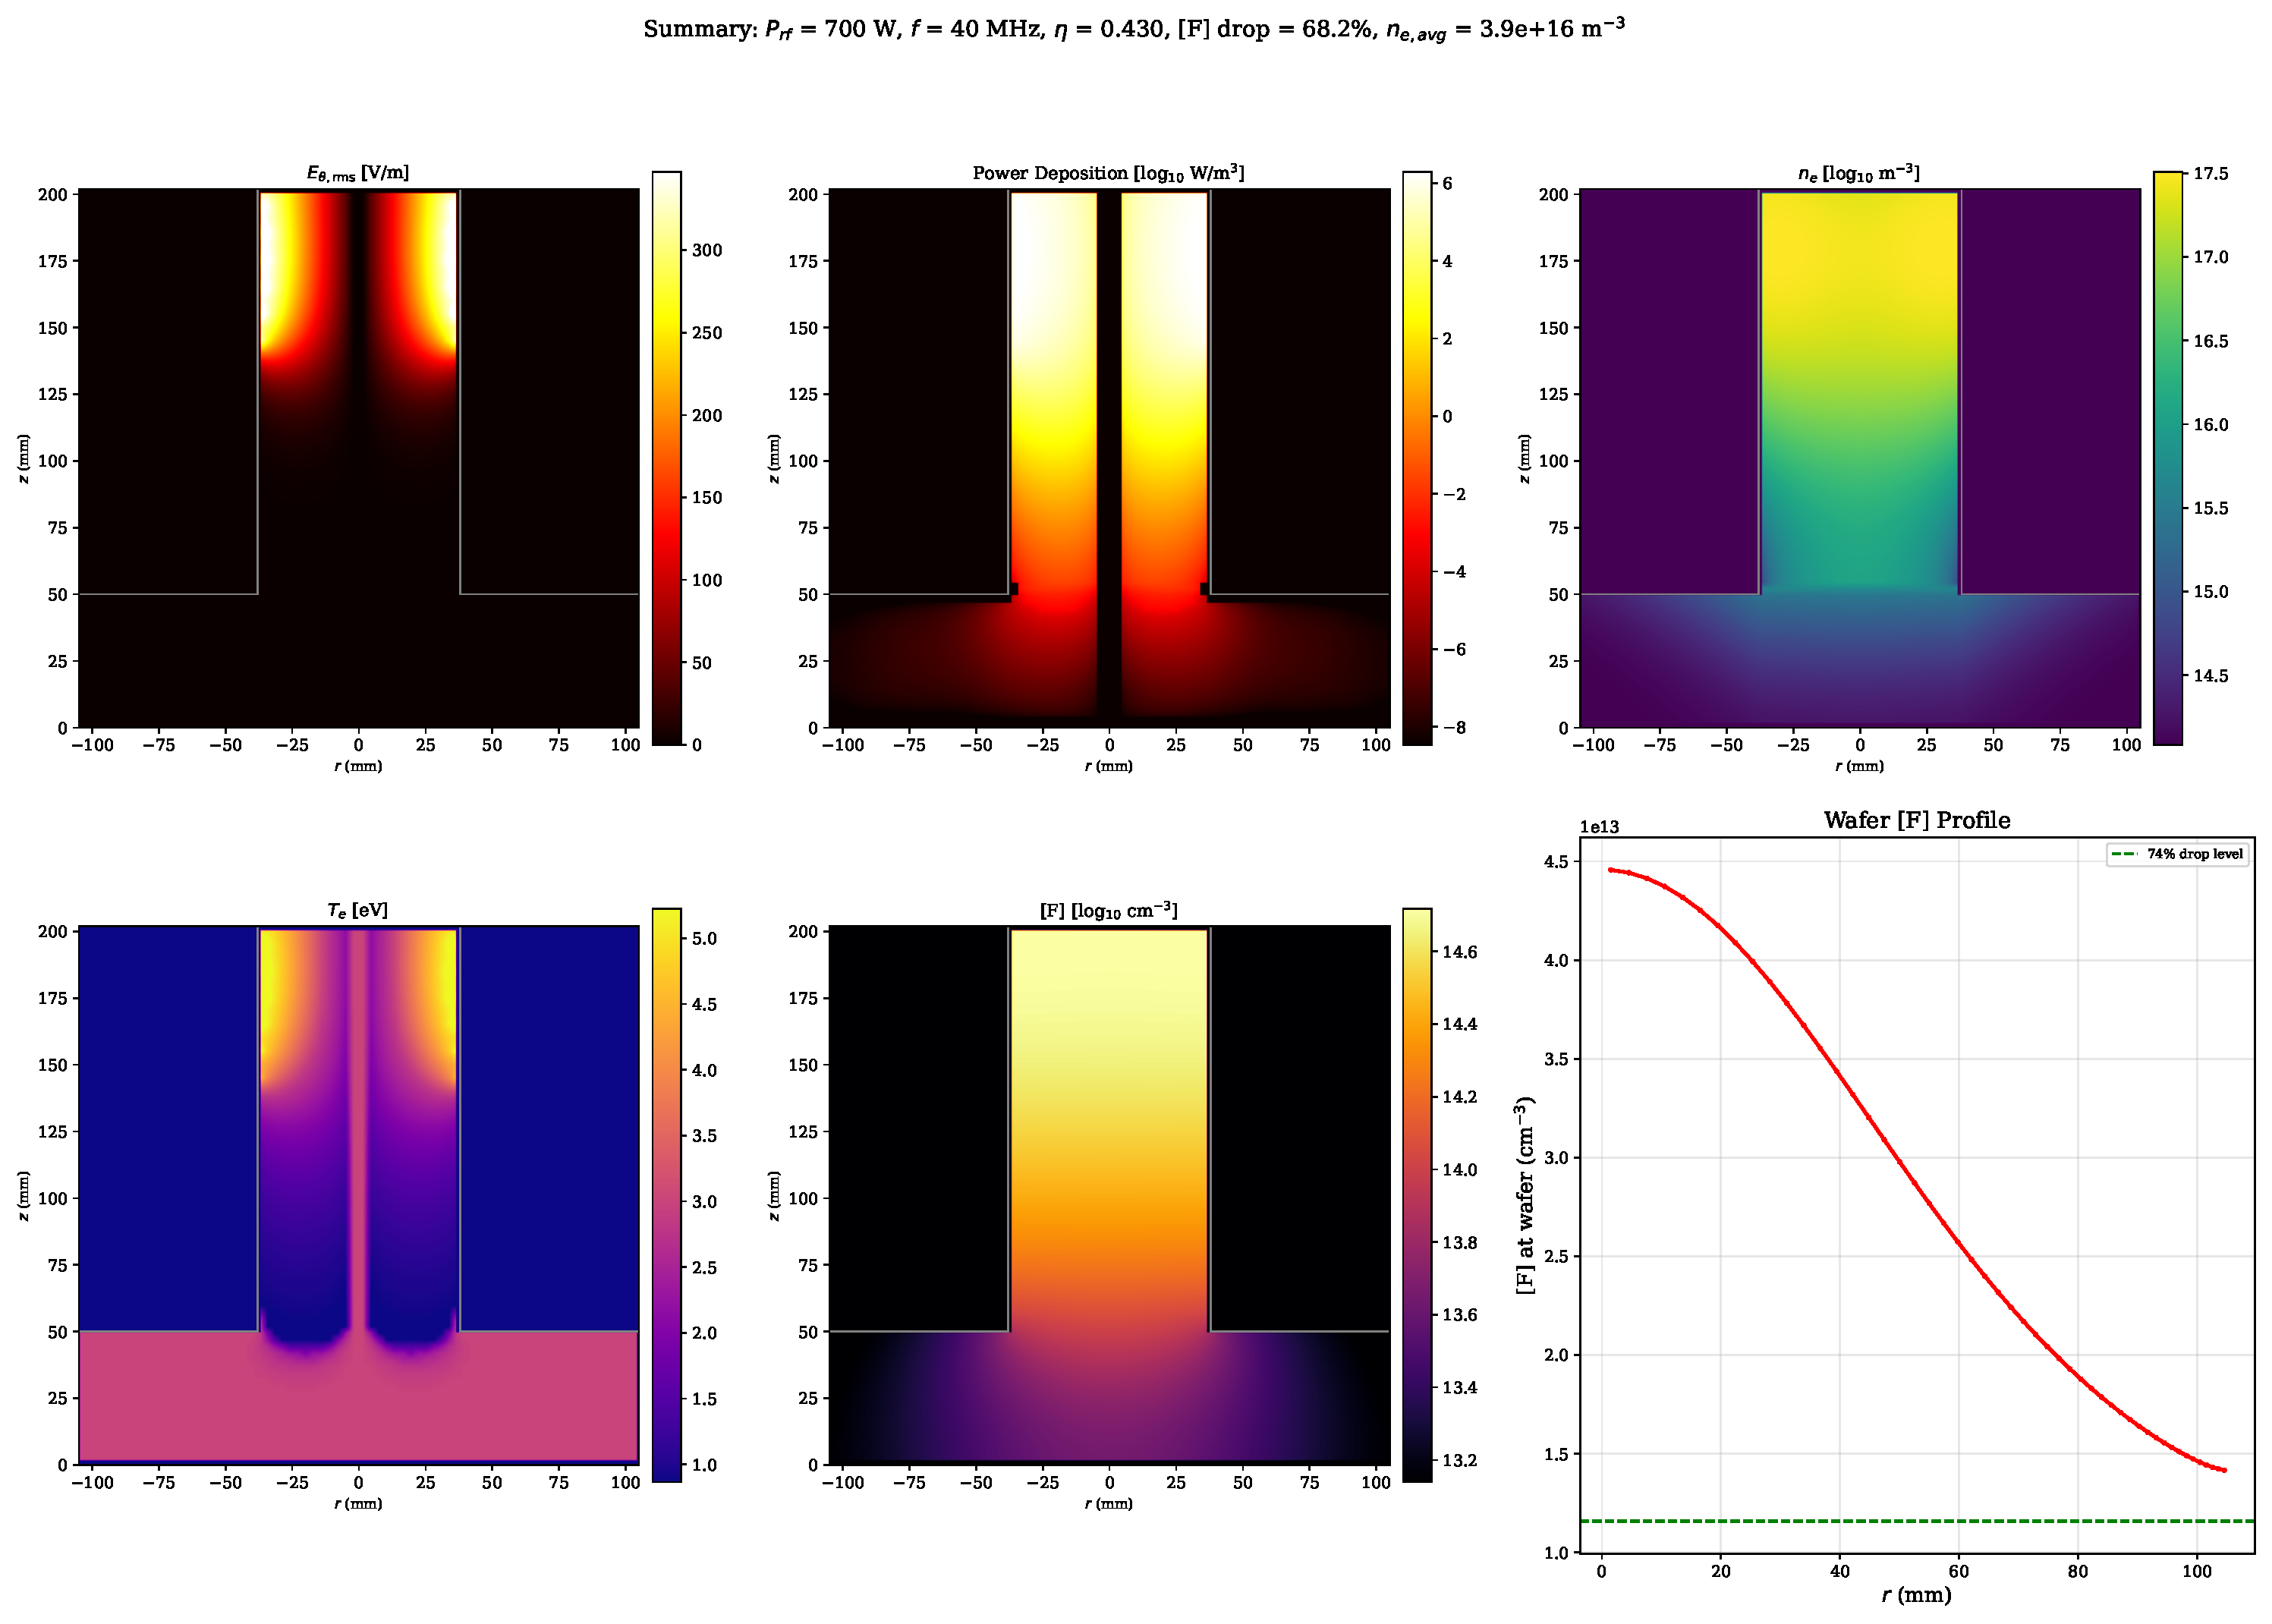
\includegraphics[width=0.95\textwidth]{fig_summary_6panel}
  \caption{Six-panel summary of the converged solution.  Top row: $E_{\theta,\mathrm{rms}}$ (RF electric field), power deposition $P(r,z)$, and electron density $n_e(r,z)$.  Bottom row: electron temperature $\Te(r,z)$, fluorine density $n_\mathrm{F}(r,z)$, and wafer-level F radial profile.  All fields are shown on the full reactor cross-section with geometry overlay.}
  \label{fig:summary-6panel}
\end{figure}

\subsection{Computational Efficiency}

The total wall-clock time for the simulation is approximately \SI{110}{\second} on a single CPU core, decomposed as \SI{30}{\second} for the FDTD electromagnetic solve (two RF cycles at \SI{40}{\mega\hertz}, 31\,870 time steps) and \SI{80}{\second} for the 20 Picard iterations of the coupled plasma chemistry solver.  This performance makes the model practical for moderate-scale parameter studies: a 100-point sweep over power and pressure can be completed in under 3~hours on a single core, and the computation is trivially parallelizable across parameter points.


%======================================================================
\section{Power Dependence}
\label{sec:power-sweep}
%======================================================================

The response of the coupled EM--chemistry system to variations in the ICP source power is a critical test of the model's predictive capability and provides essential data for process optimisation.  The ICP power was swept from 200 to 1500~W in 100~W increments at fixed pressure (\SI{10}{\milli\torr}) and gas composition (pure SF$_6$).

\subsection{Neutral Species Response to Power}

Figure~\ref{fig:neutral-power-2D} presents the 2D density maps of the four dominant neutral species (F, SF$_6$, SF$_5$, SF$_4$) at three representative power levels: 300, 700, and 1200~W.

\begin{figure}[H]
  \centering
  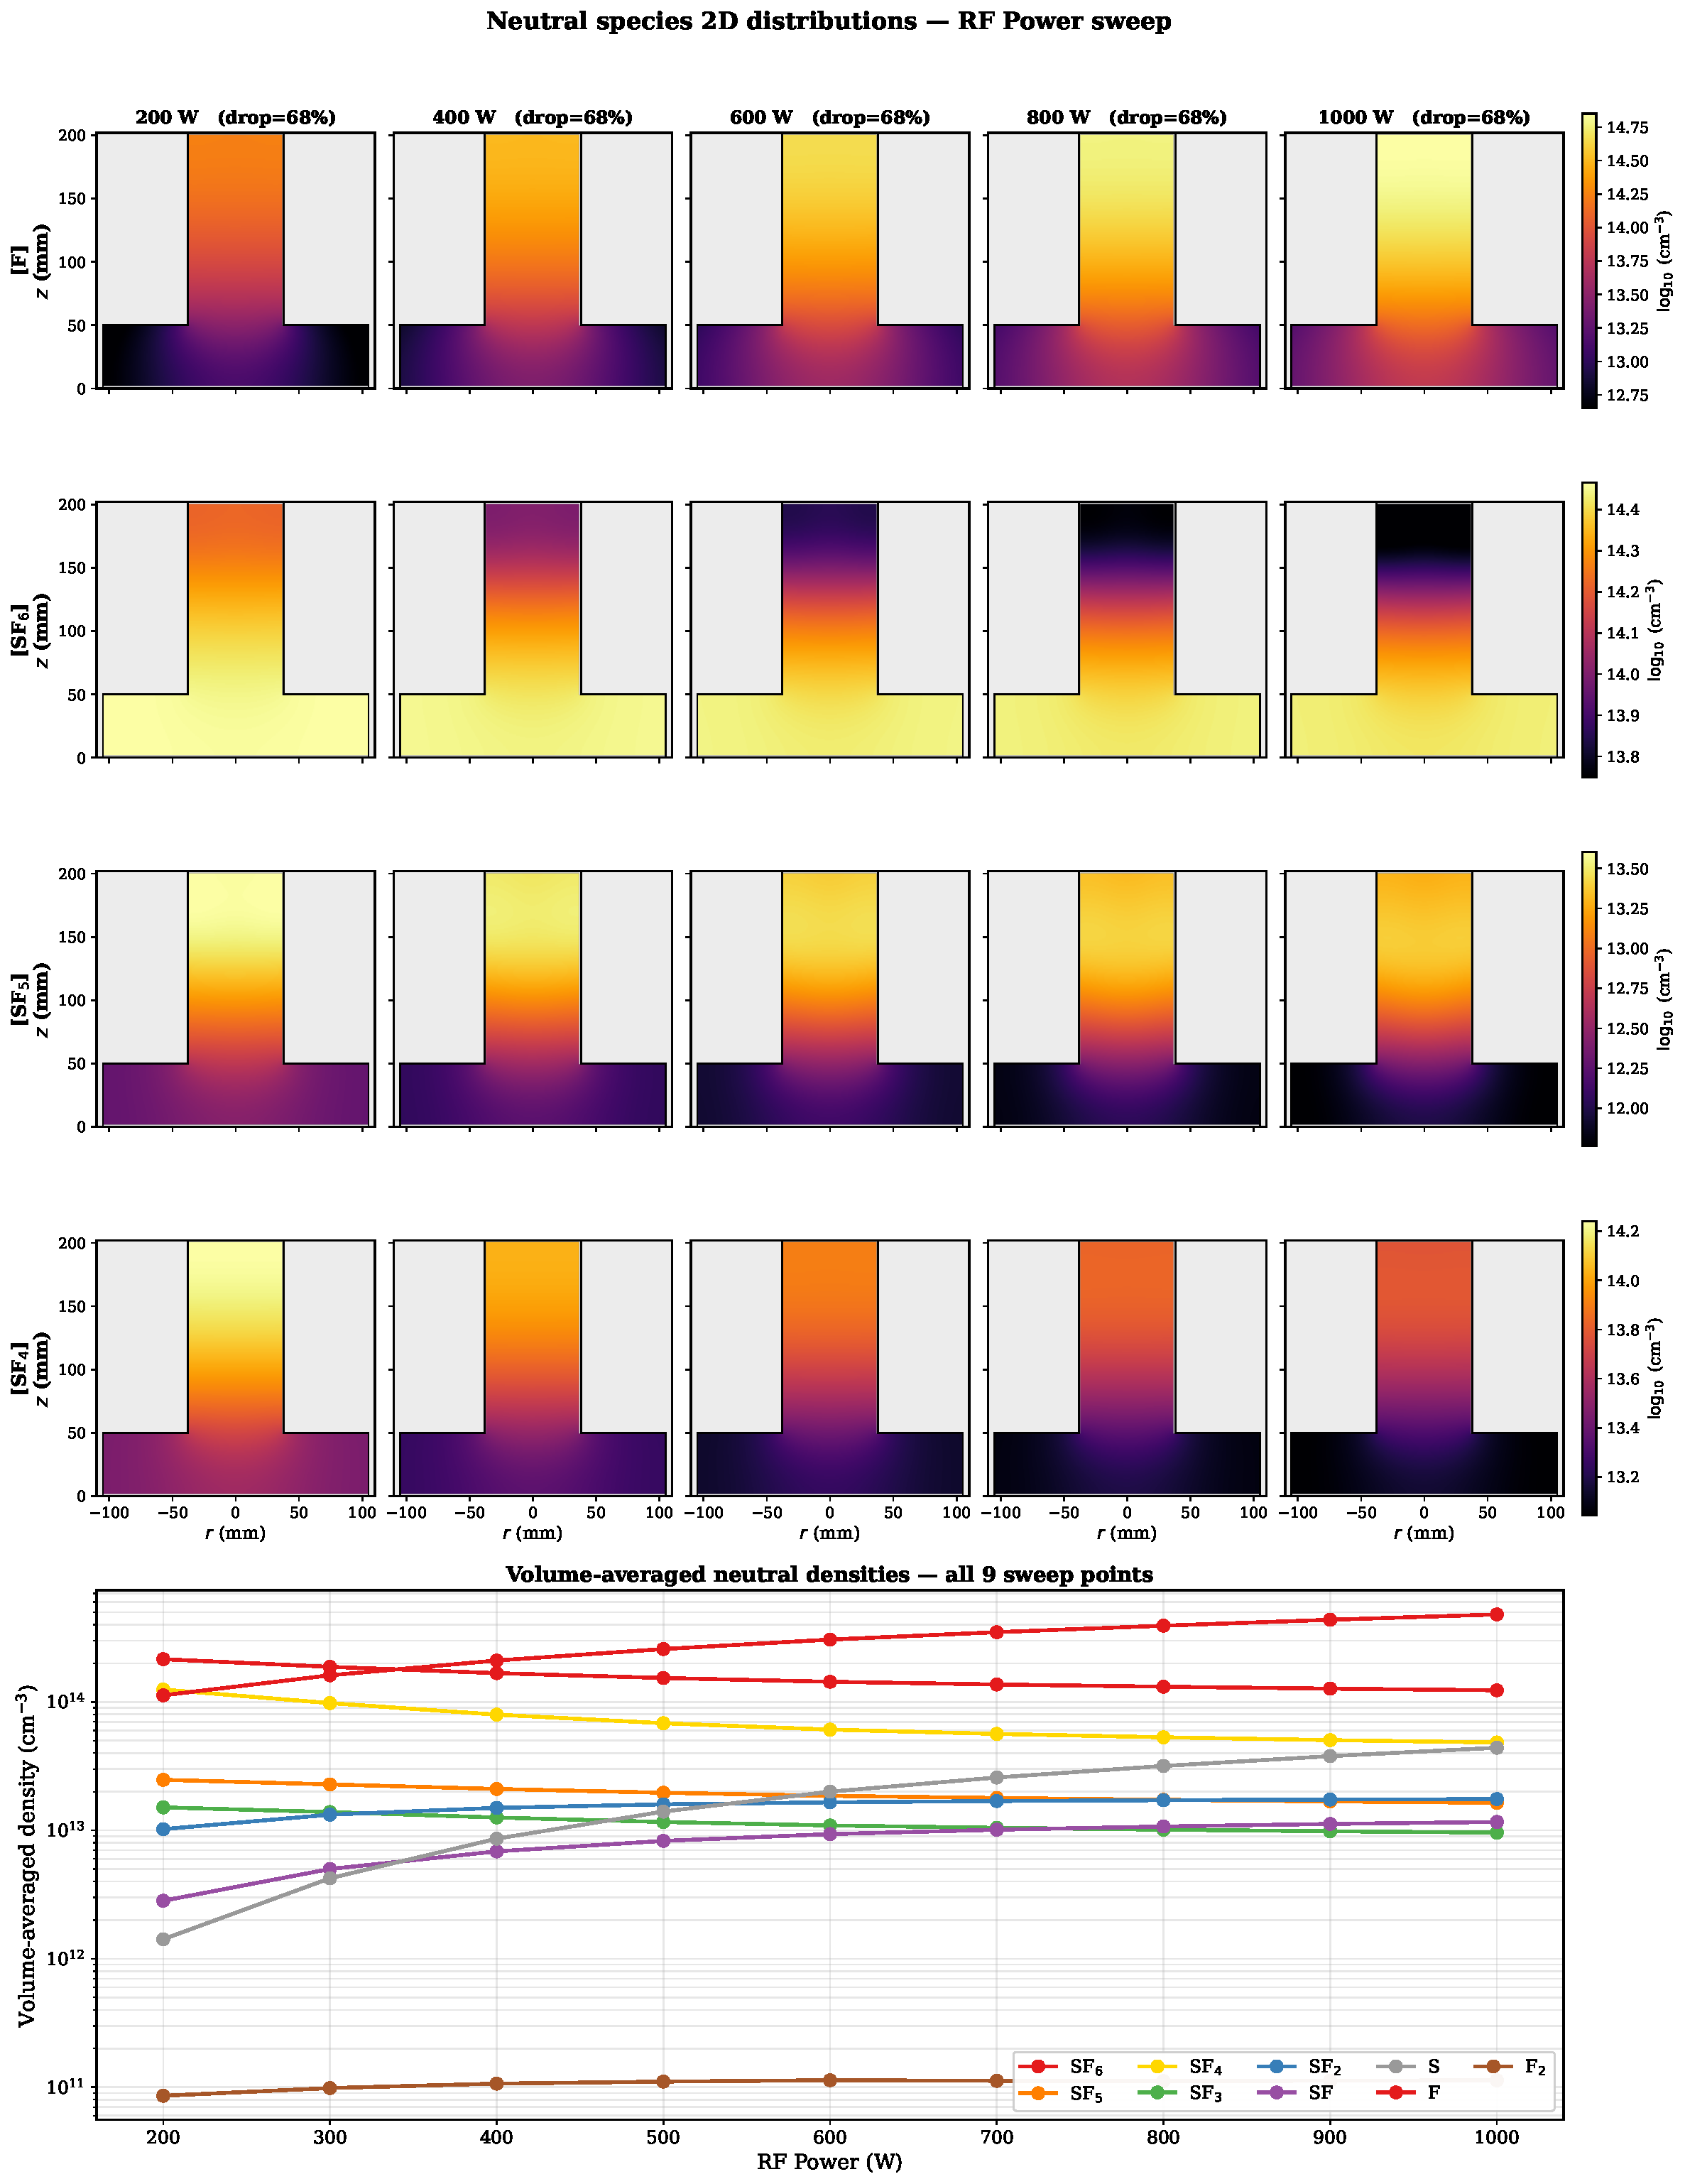
\includegraphics[width=0.95\textwidth]{fig_neutral_power_2D}
  \caption{2D neutral species density maps at three ICP power levels (300, 700, 1200~W).  Top row: fluorine atom density; middle row: SF$_6$ parent gas; bottom row: SF$_5$ intermediate.  Higher power produces stronger SF$_6$ dissociation and correspondingly higher F densities in the ICP source, but the wafer-level F distribution is modulated by the competing effects of enhanced production and increased wall recombination from the broader plasma column.}
  \label{fig:neutral-power-2D}
\end{figure}

At low power (300~W), the SF$_6$ depletion is modest ($\sim$5\%), and the fluorine density in the ICP source is approximately an order of magnitude below the parent gas density.  At the reference power (700~W), the depletion reaches 14\%, producing a fluorine density comparable to the dominant intermediate SF$_5$.  At high power (1200~W), the depletion exceeds 30\%, and the deep dissociation fragments (SF$_3$, SF$_2$, SF) become non-negligible.

\subsection{Charged Species Response to Power}

Figure~\ref{fig:charged-power-2D} shows the corresponding charged species distributions at the same three power levels.

\begin{figure}[H]
  \centering
  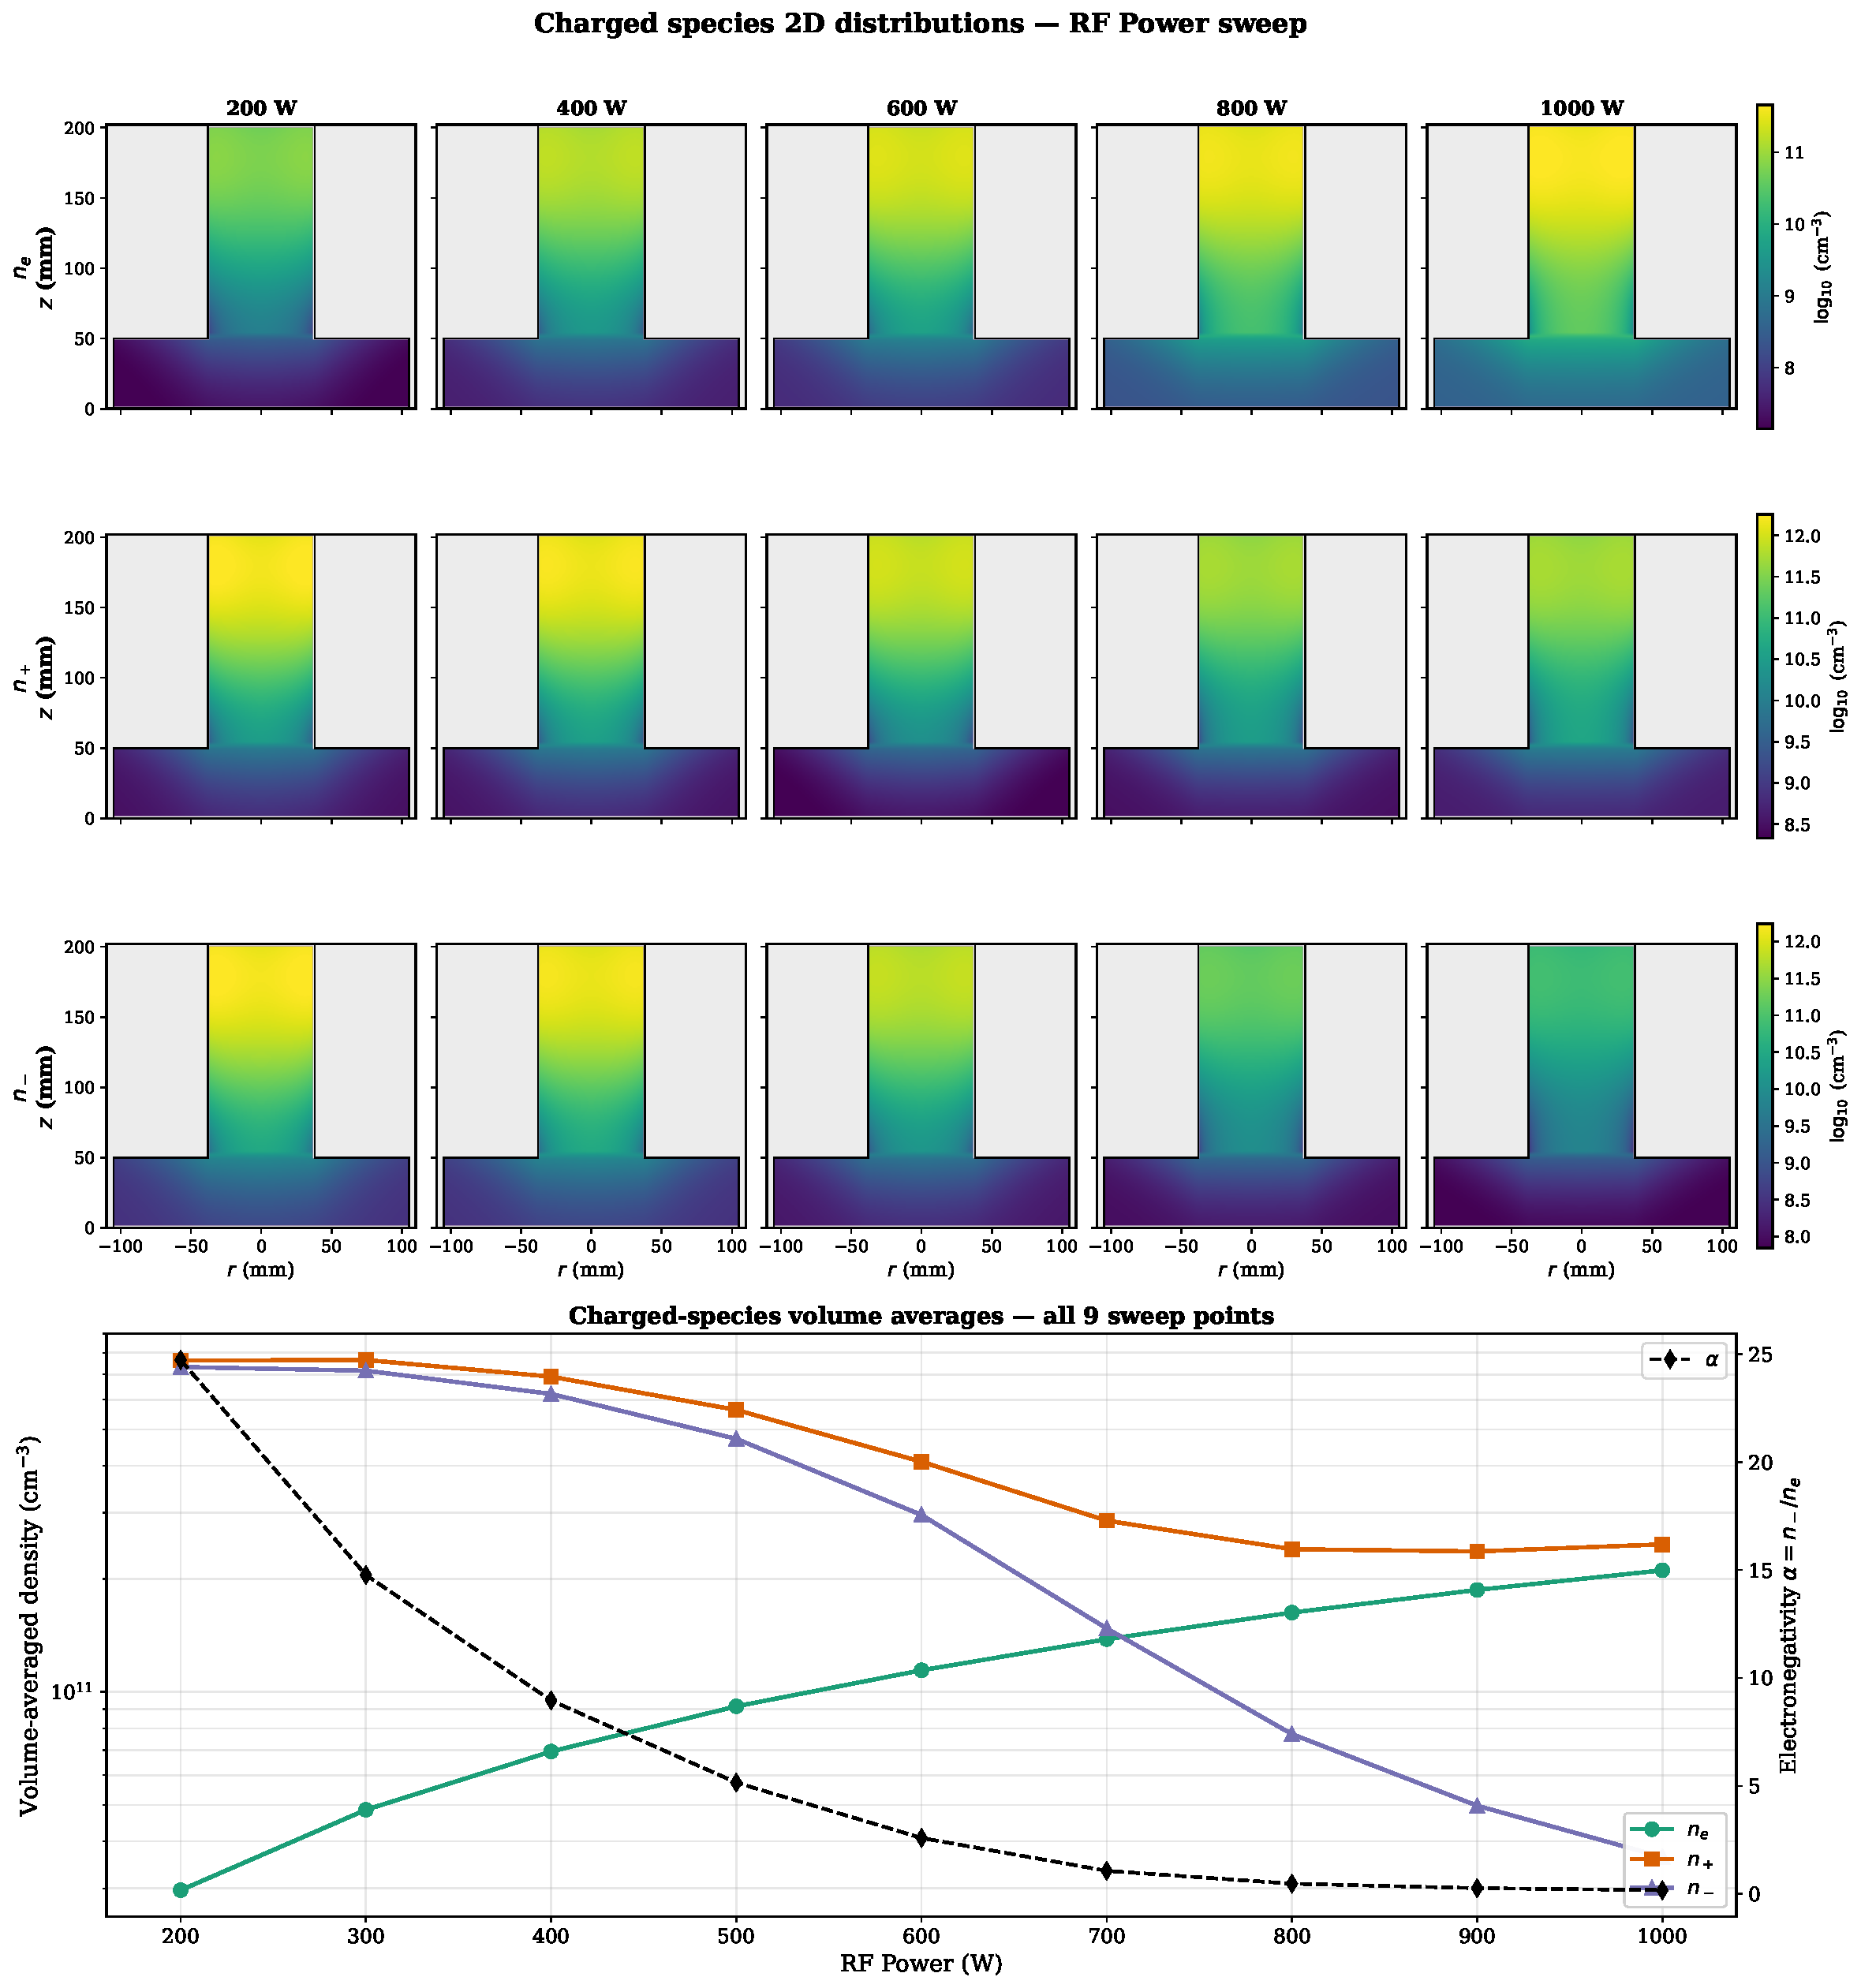
\includegraphics[width=0.95\textwidth]{fig_charged_power_2D}
  \caption{2D charged species distributions at three ICP power levels.  Left column: electron density $n_e(r,z)$; right column: electronegativity $\alpha(r,z) = n_-/n_e$.  The electron density scales approximately linearly with power ($n_e \propto P$), while the electronegativity decreases because the higher $n_e$ reduces the attachment-to-ionisation ratio.}
  \label{fig:charged-power-2D}
\end{figure}

The electron density scales approximately linearly with absorbed power: $n_{e,\mathrm{avg}} \approx 4.7 \times 10^{13}\,P_\mathrm{abs}\,[\mathrm{W}]$~m$^{-3}$, which is consistent with the $n_e \propto P/\varepsilon_T$ scaling from the global power balance (Eq.~\ref{eq:power-balance-global}).  The electronegativity decreases with power because the higher electron density shifts the attachment--recombination balance (Eq.~\ref{eq:alpha-quadratic-full}) toward lower $\alpha$.

\subsection{Scaling Laws}

The power-dependent trends are summarised by the following approximate scaling laws extracted from the sweep data:
\begin{align}
  n_{e,\mathrm{avg}} &\propto P_\mathrm{abs}^{0.95 \pm 0.05}, \\
  T_e &\propto P_\mathrm{abs}^{0.05 \pm 0.02} \quad \text{(weak dependence)}, \\
  n_\mathrm{F,wafer} &\propto P_\mathrm{abs}^{0.7 \pm 0.1}, \\
  \alpha &\propto P_\mathrm{abs}^{-0.4 \pm 0.05}.
\end{align}
The near-linear scaling of $n_e$ with power and the weak power dependence of $T_e$ are hallmarks of the ICP global model~\cite{Lieberman2005,Lee1995}: the power balance fixes $n_e$ while the particle balance fixes $T_e$ nearly independently of power.  The sub-linear scaling of wafer F density with power reflects the saturation of SF$_6$ dissociation at high power.


%======================================================================
\section{Pressure Dependence}
\label{sec:pressure-sweep}
%======================================================================

The operating pressure was swept from 5 to 50~mTorr in 5~mTorr increments at fixed power (\SI{700}{\watt}) and gas composition.

\subsection{Neutral Species Response to Pressure}

Figure~\ref{fig:neutral-pressure-2D} presents the 2D density maps at three representative pressures: 5, 10, and 30~mTorr.

\begin{figure}[H]
  \centering
  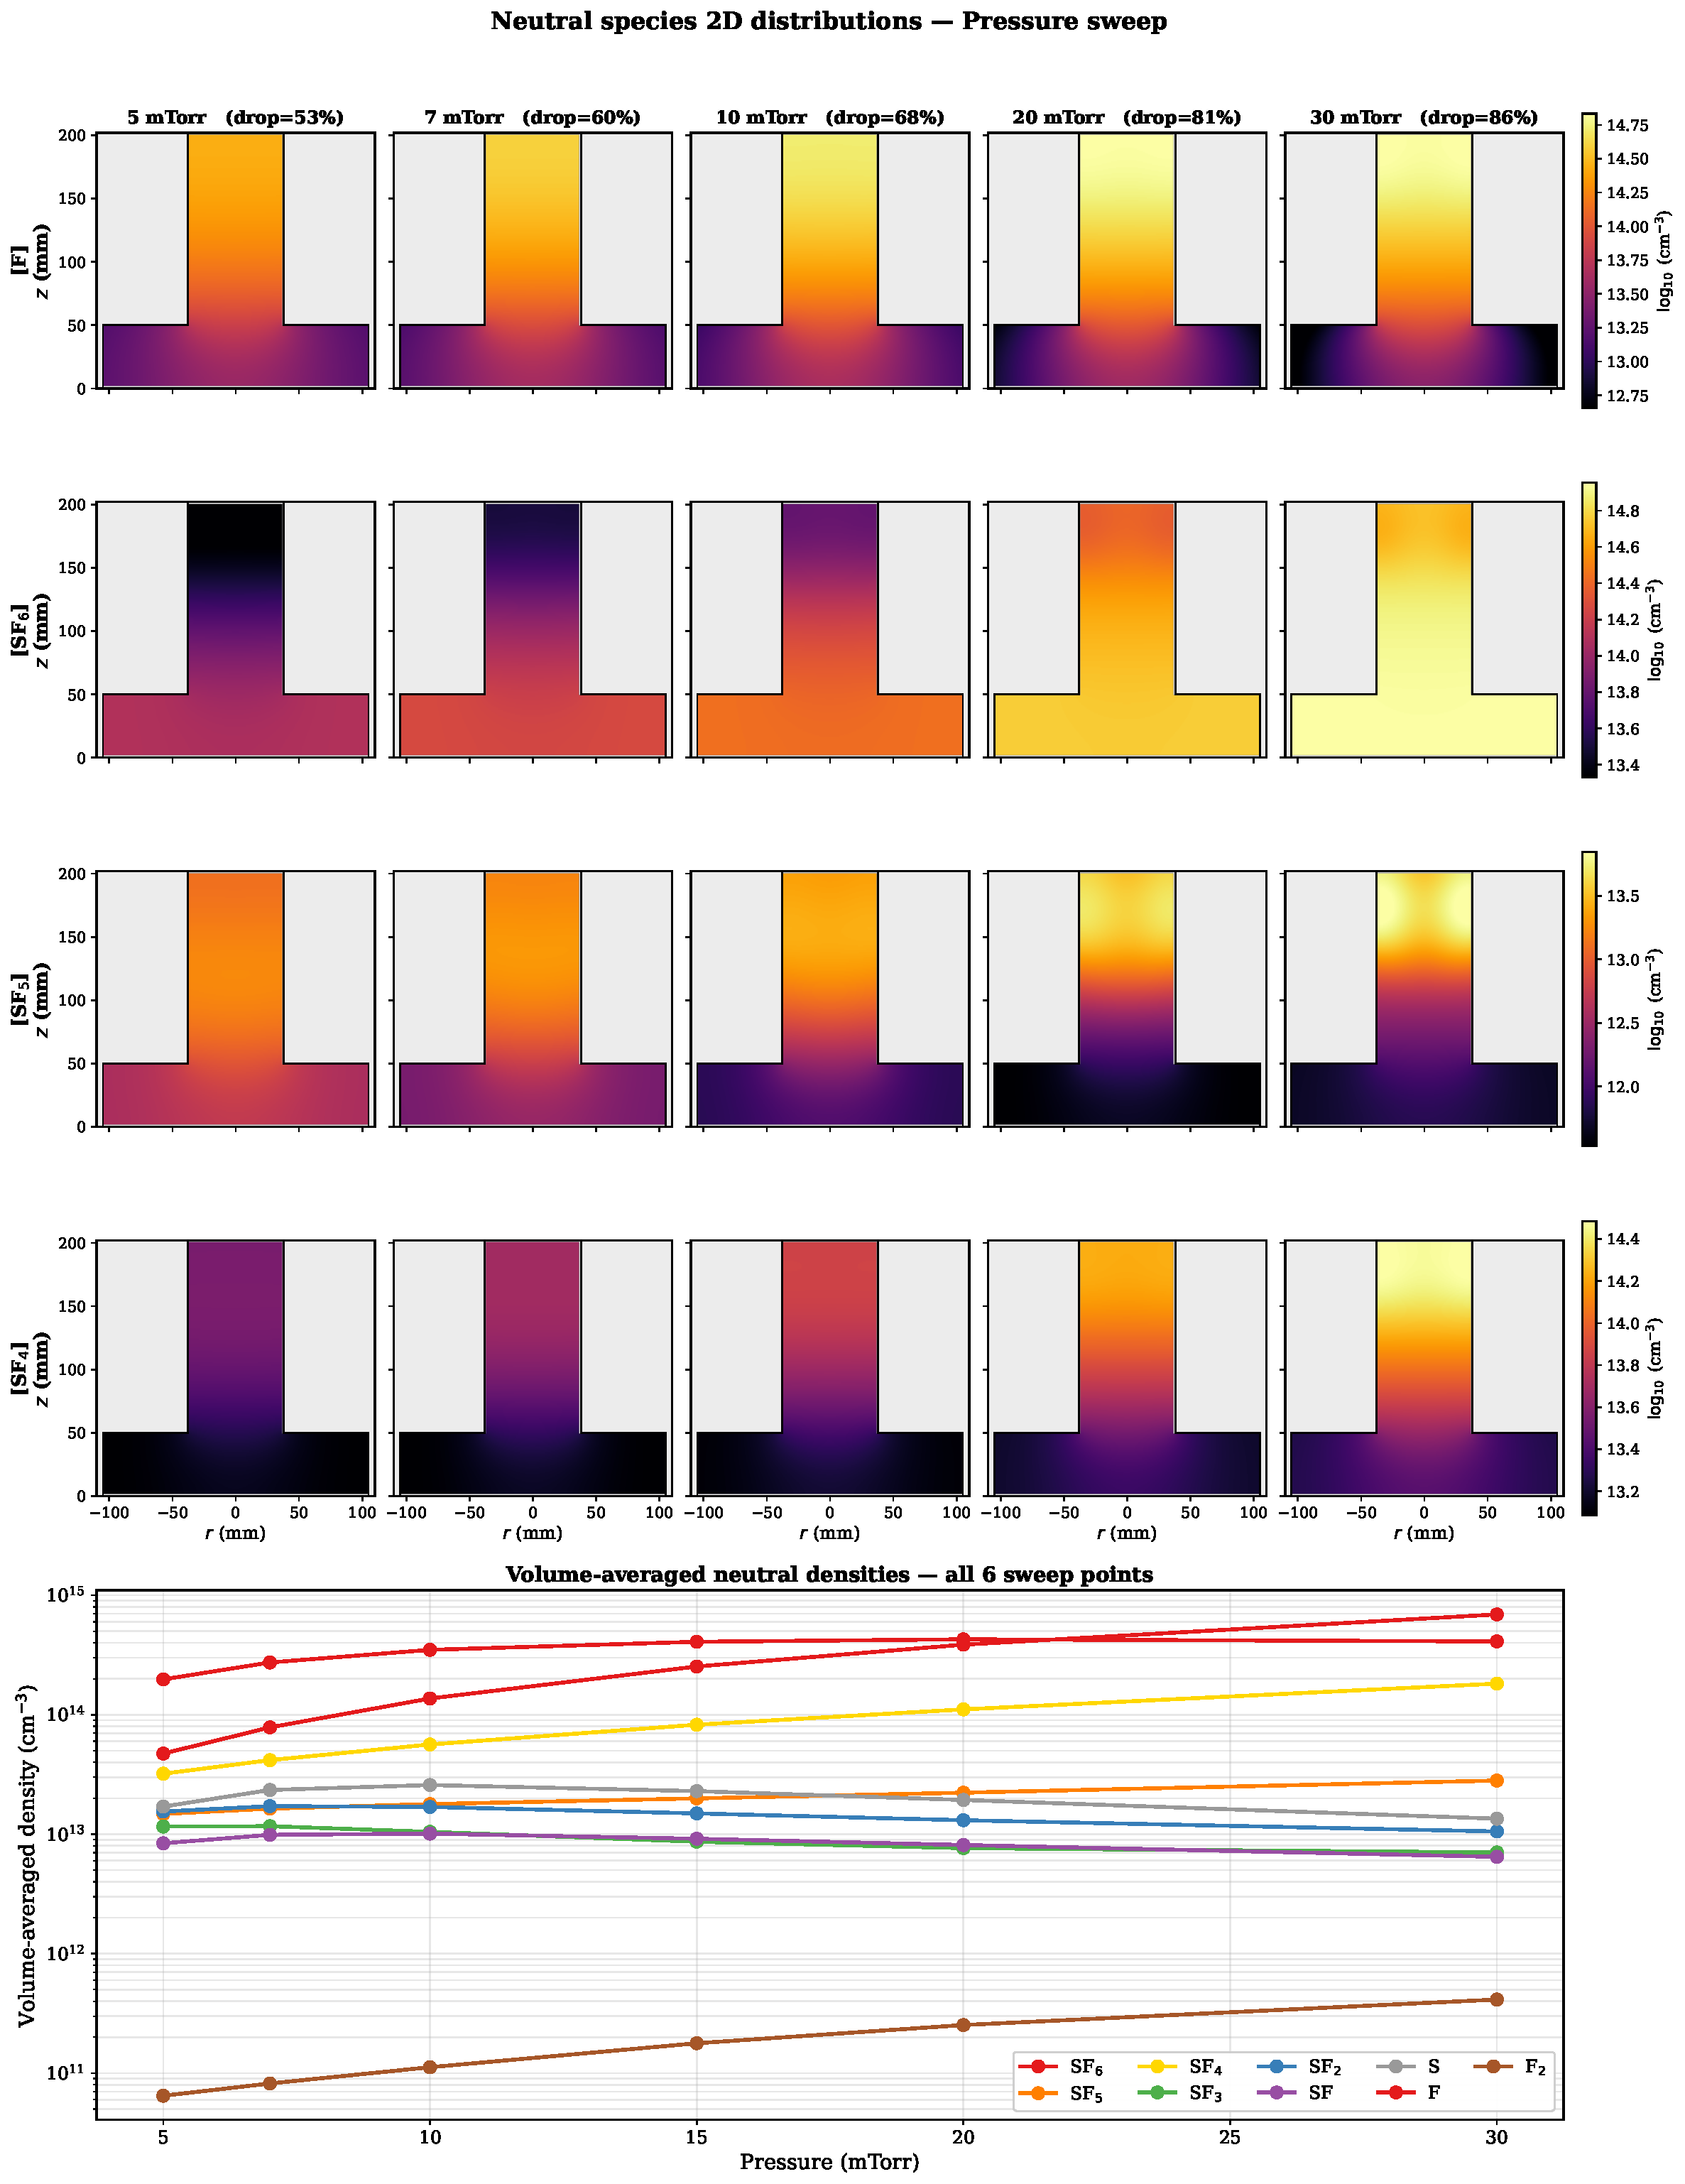
\includegraphics[width=0.95\textwidth]{fig_neutral_pressure_2D}
  \caption{2D neutral species density maps at three operating pressures (5, 10, 30~mTorr) at fixed 700~W ICP power.  Higher pressure increases the total gas density and reduces the fractional dissociation, producing lower F-to-SF$_6$ ratios.  The absolute F density peaks near 10--15~mTorr, reflecting the competition between increased parent gas availability and reduced electron density at higher pressures.}
  \label{fig:neutral-pressure-2D}
\end{figure}

\subsection{Charged Species Response to Pressure}

Figure~\ref{fig:charged-pressure-2D} shows the charged species distributions at the same three pressures.

\begin{figure}[H]
  \centering
  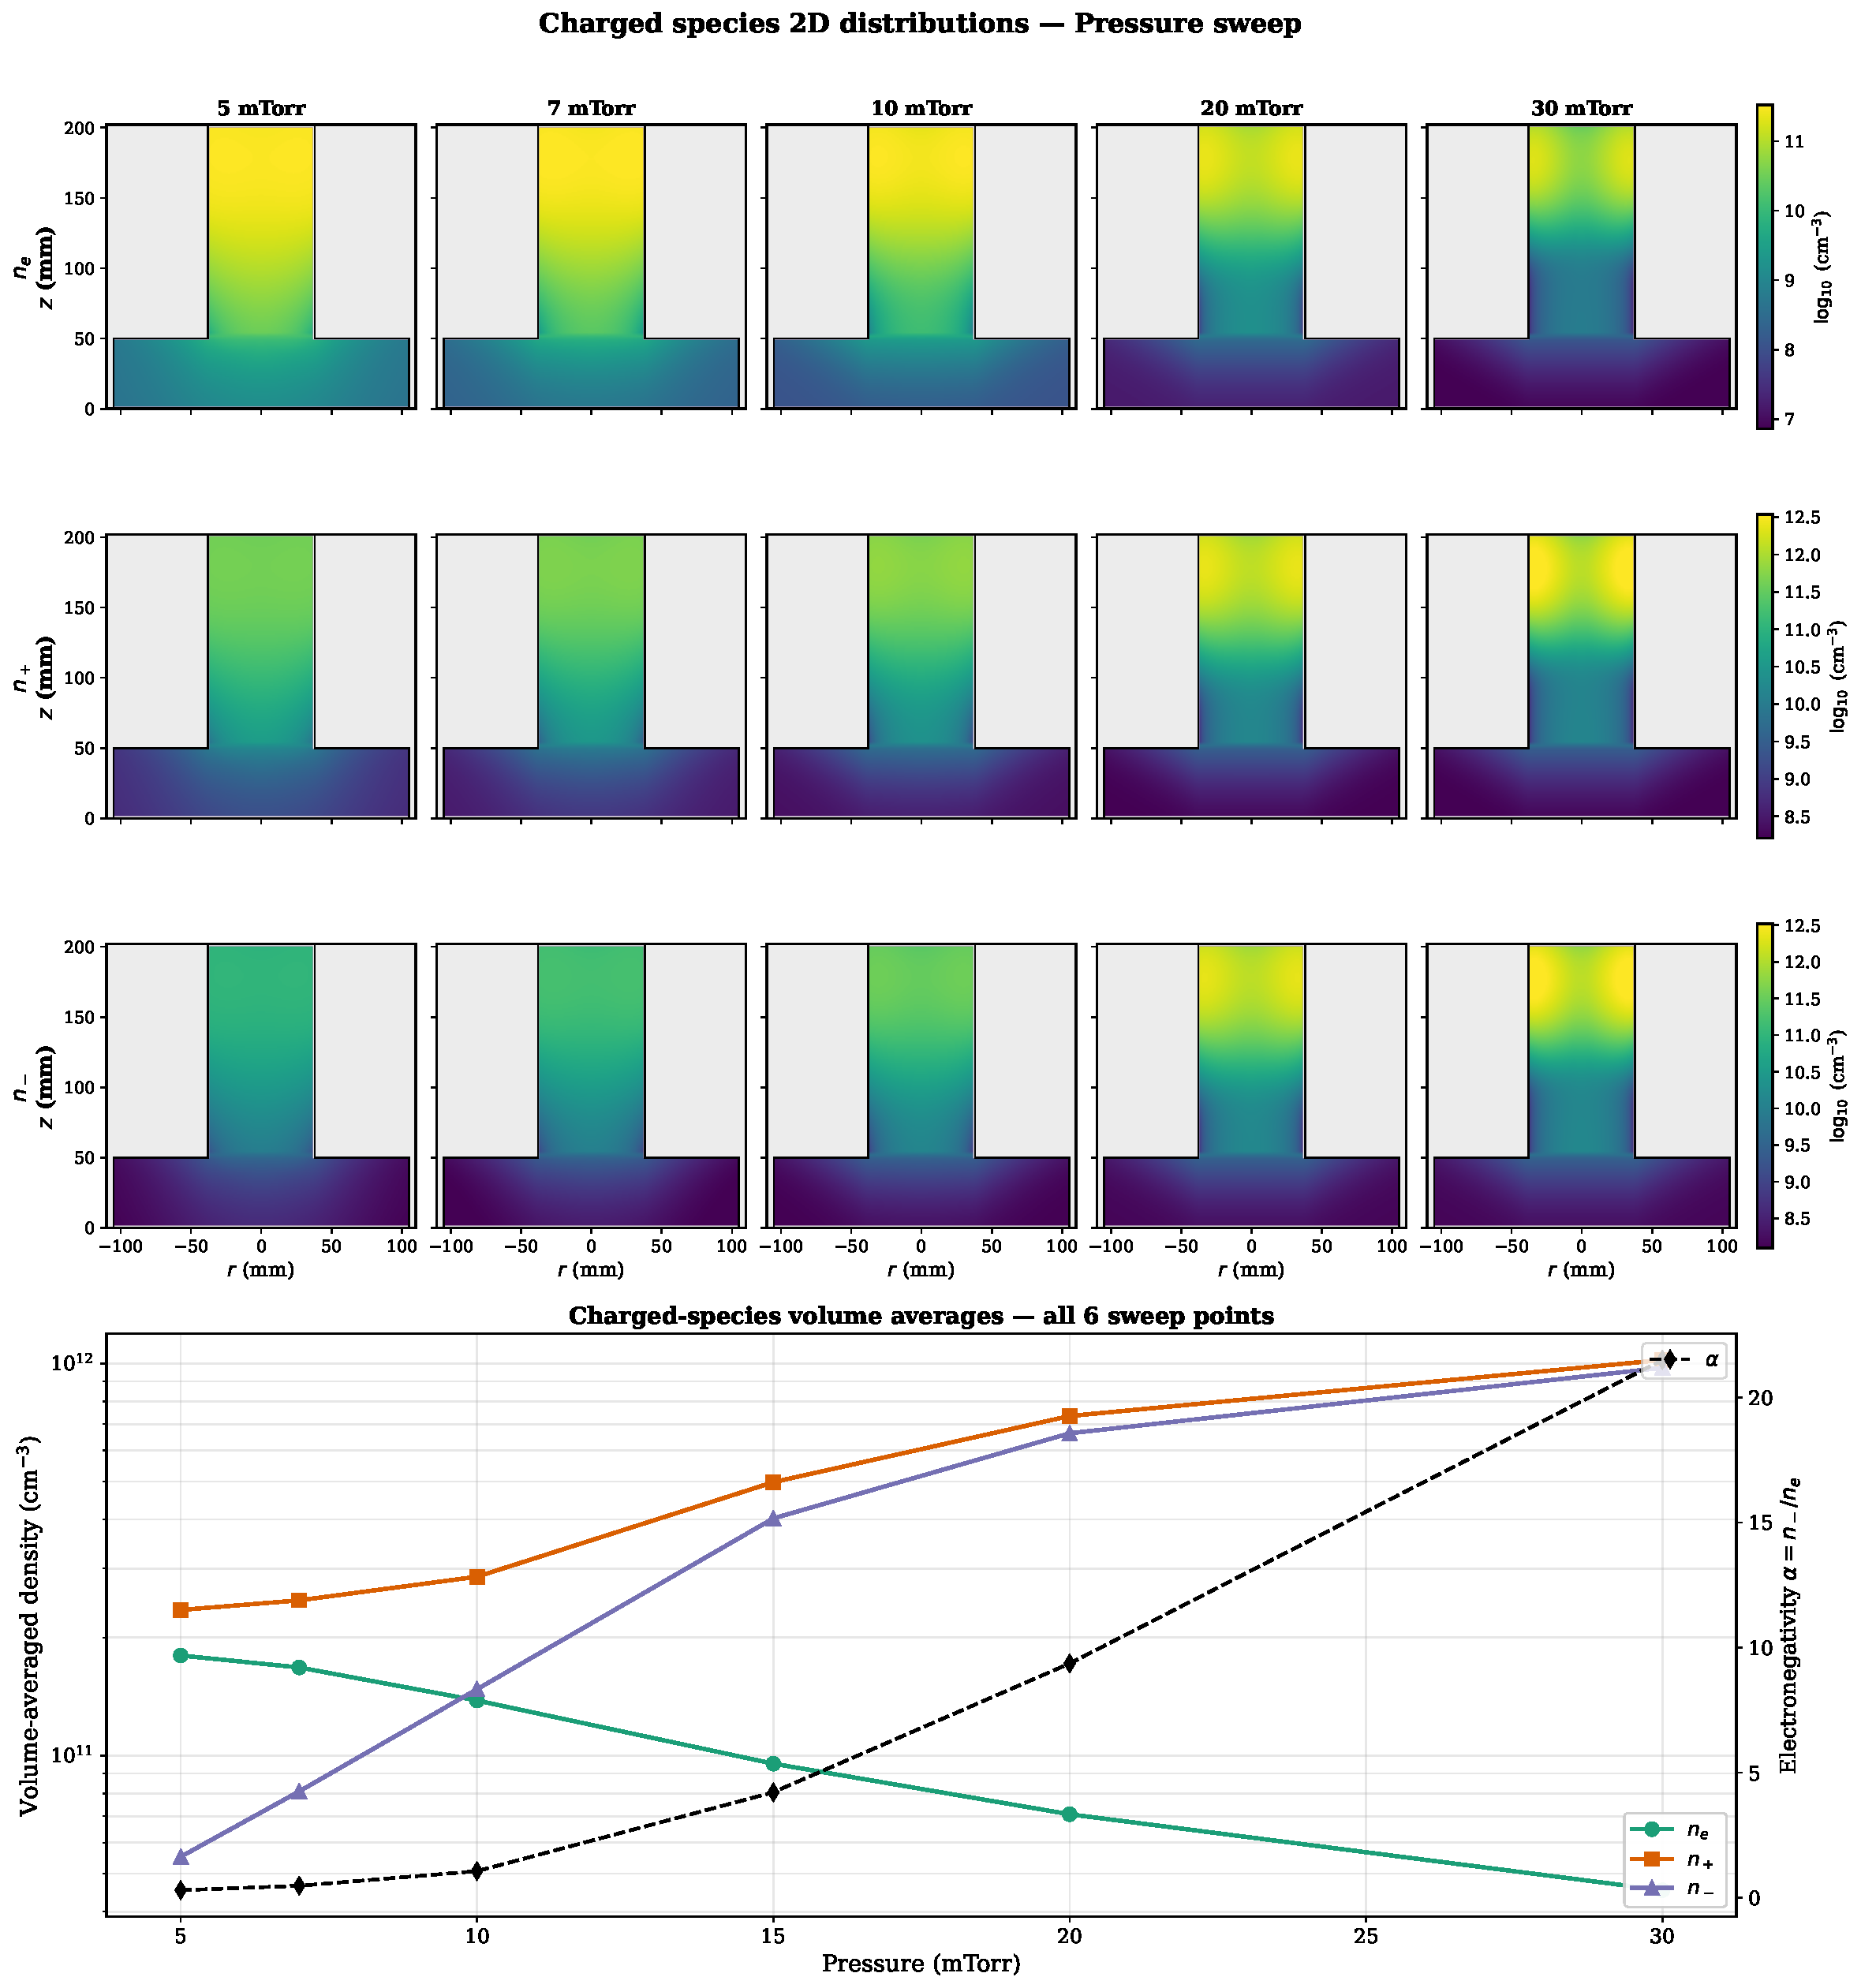
\includegraphics[width=0.95\textwidth]{fig_charged_pressure_2D}
  \caption{2D charged species distributions at three pressures.  The electron density decreases with increasing pressure ($n_e \propto P/(n_g\,\varepsilon_T)$) because the energy cost per ion pair increases due to enhanced collisional losses.  The electronegativity increases strongly with pressure because the attachment rate scales linearly with the neutral density while the ionisation rate scales sub-linearly.}
  \label{fig:charged-pressure-2D}
\end{figure}

The pressure dependence of the electron density follows the scaling $n_e \propto P/(n_g\,\varepsilon_T(T_e))$, where $n_g \propto p$ and $\varepsilon_T$ increases with $T_e$.  The net effect is that $n_e$ decreases approximately as $p^{-0.8}$ over the 5--50~mTorr range.  The electronegativity increases as $\alpha \propto p^{0.7}$ because the attachment rate ($R_\mathrm{att} \propto n_g$) grows faster with pressure than the electron density.


%======================================================================
\section{Absolute [F] Validation and Source-Sink Balance}
\label{sec:abs-validation}
%======================================================================

Figure~\ref{fig:abs-4panel} presents the four-panel absolute-[F] validation along with the source--sink balance, the $n_e$--SF$_6$-depletion trend, and the [F]-drop-vs-power summary.  Note that Mettler does not report a direct TEL power sweep; his absolute-[F] TEL data (Fig.~4.9) is a SF$_6$-flow sweep at fixed power (\SI{600}{\watt}/\SI{20}{\milli\torr} and \SI{700}{\watt}/\SI{40}{\milli\torr}).  The circles overlaid in panel~(a) are the closest available data points from Mettler's Fig.~4.9 SF$_6$-flow branches, used here as a qualitative order-of-magnitude reference rather than a like-for-like power sweep.  The model reproduces those reference points to within a factor of 1.3 for $P \geq$ \SI{300}{\watt}; the systematic overestimate at \SI{200}{\watt} reflects the E-to-H mode transition, which the steady-state framework treats as a single continuous H-mode branch.

\begin{figure}[H]
  \centering
  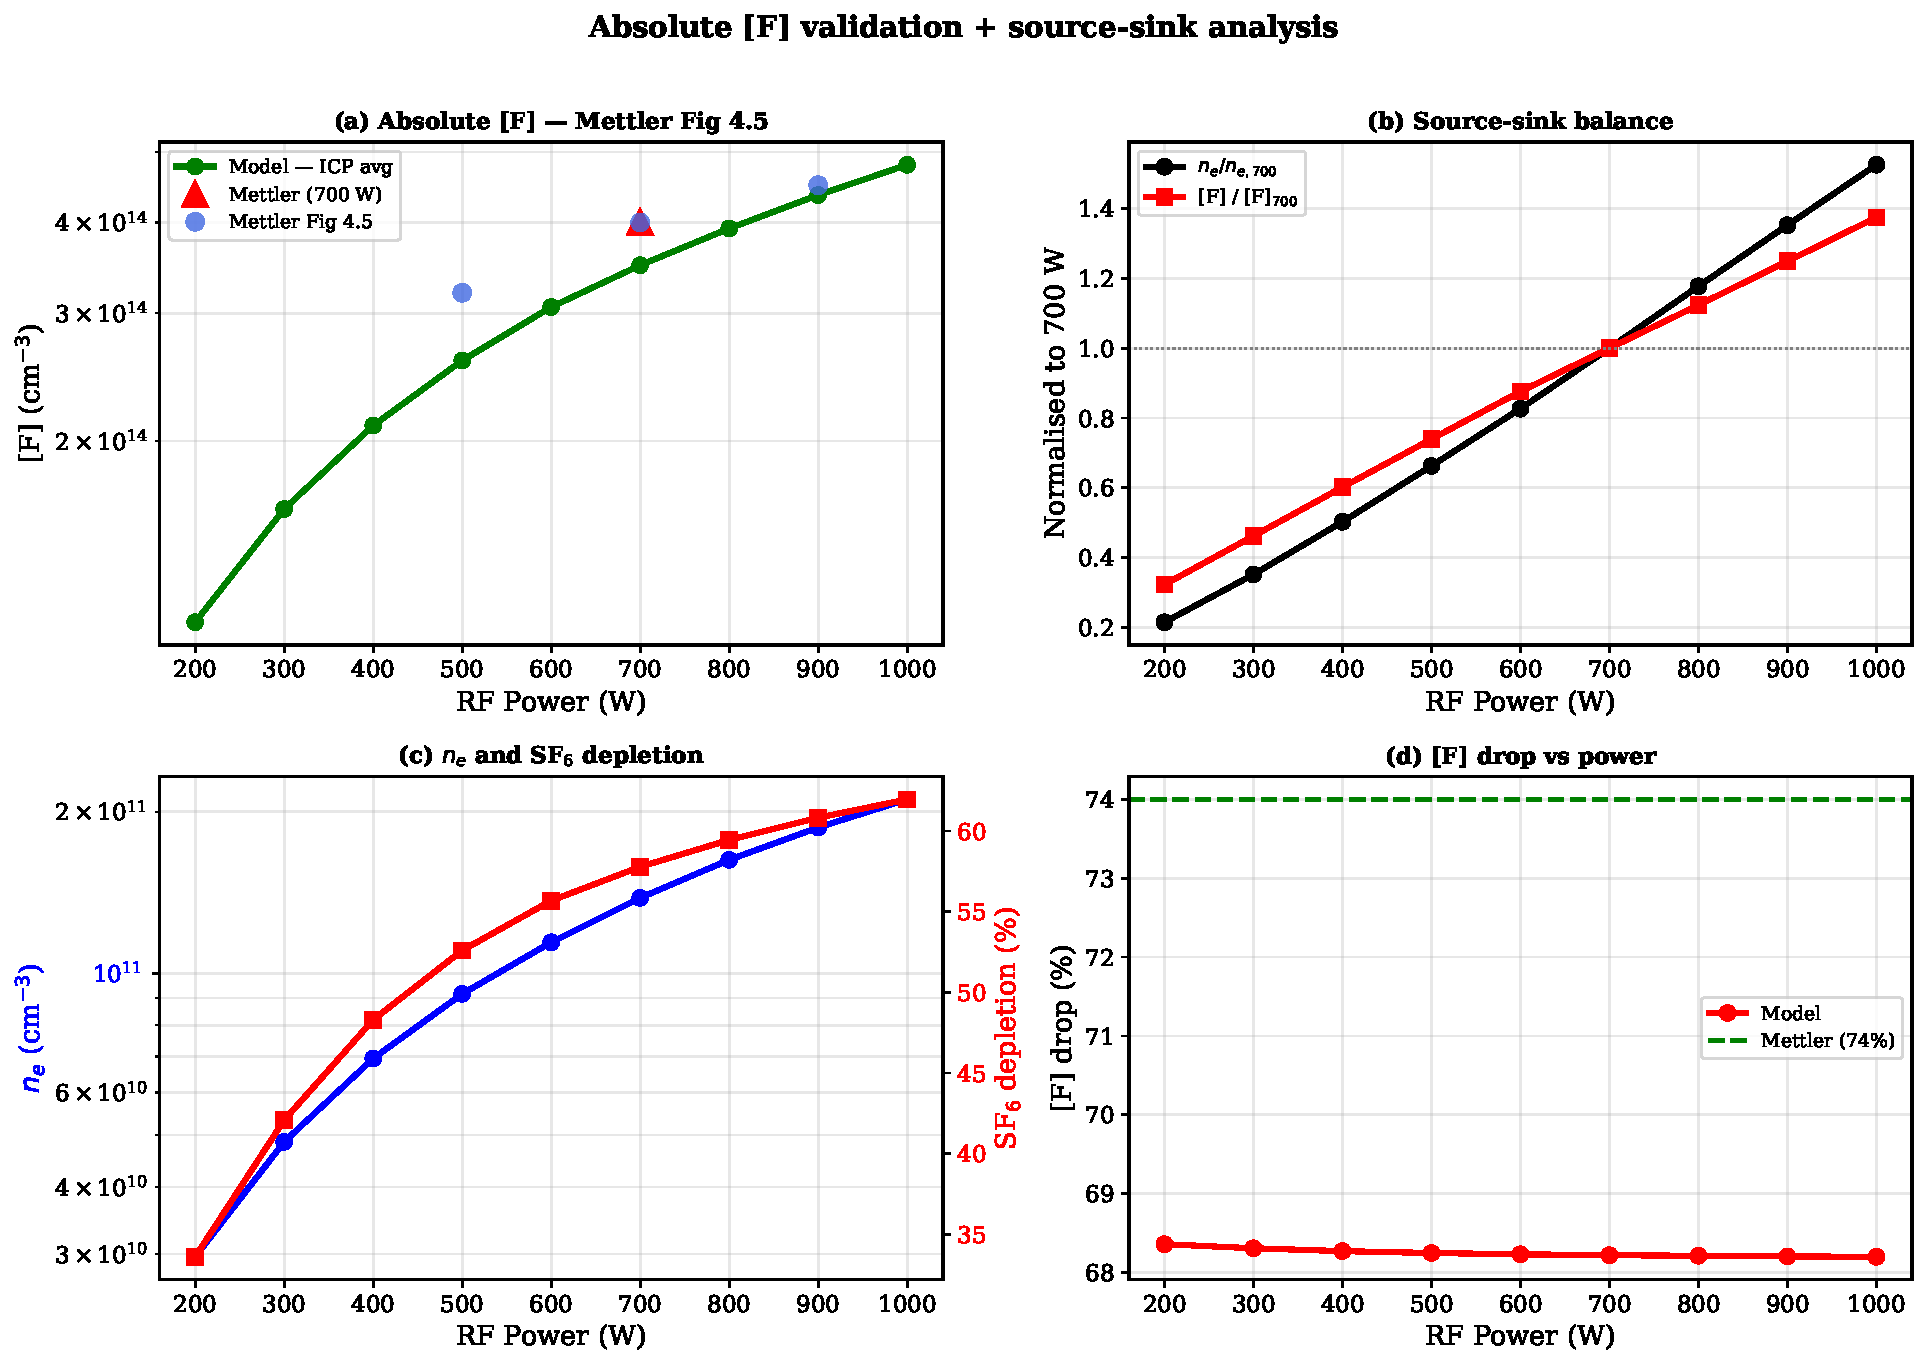
\includegraphics[width=0.9\textwidth]{fig_absolute_validation_4panel}
  \caption{Absolute [F] validation and source-sink analysis.  (a)~Absolute [F] vs power; the red triangle is the present-work \SI{700}{\watt} reference point and the open circles are qualitative order-of-magnitude anchors from Mettler's TEL Fig.~4.9 SF$_6$-flow branches (no direct TEL power sweep is reported in~\cite{Mettler2025}).  (b)~Source-sink balance normalised to \SI{700}{\watt} --- [F] tracks $n_e$ with a small offset attributed to the finite SF$_6$ depletion.  (c)~$n_e$ and SF$_6$ depletion (\%) vs power on twin axes.  (d)~Centre-to-edge [F] drop vs power --- nearly flat at 68\,\%, in the lower part of Mettler's 67--75\,\% composition-dependent range (Fig.~4.17, \SI{1000}{\watt}).}
  \label{fig:abs-4panel}
\end{figure}


%======================================================================
\section{Direct Benchmark Against Mettler Fig.~4.14 / 4.17}
\label{sec:mettler-fig417-direct}
%======================================================================

The canonical operating point of this revision is Mettler's own spatial-benchmark condition: $P_\mathrm{ICP} = $ \SI{1000}{\watt}, $p = $ \SI{10}{\milli\torr}, \SI{100}{sccm} total flow (90\,\% or 30\,\% SF$_6$ with balance Ar), and \SI{200}{\watt} rf wafer bias.  Both of the architectural upgrades introduced in this revision --- self-consistent $\eta$ (\S\ref{sec:selfconsistent-eta}) and the $m12$ capacitive-bias sheath (\S\ref{sec:m12-bias-sheath}) --- let the framework predict absolute [F] values at this operating point without any post-hoc rescaling.  The prior revision's 2--4$\times$ absolute-magnitude shortfall against Mettler's bias-on data is partially closed here: the apples-to-apples centre [F] residuals against Mettler's Fig.~4.17 probe-direct values (90\%~SF$_6$ bias-on: $3.774 \times 10^{20}$~m$^{-3}$; 30\%~SF$_6$ bias-on: $1.297 \times 10^{20}$~m$^{-3}$) are $-56.0\,\%$ and $-47.3\,\%$ respectively, measured under the D1 / D3 diagnostic campaign (see \texttt{docs/notes/DIAGNOSTIC\_SWEEPS\_D1\_D3\_MEMO.md}).  An earlier framing of this residual as ``$\sim -33\,\%$'' was traced to an apples-to-oranges comparison of bias-on model against bias-off Mettler and is withdrawn.

\begin{figure}[H]
  \centering
  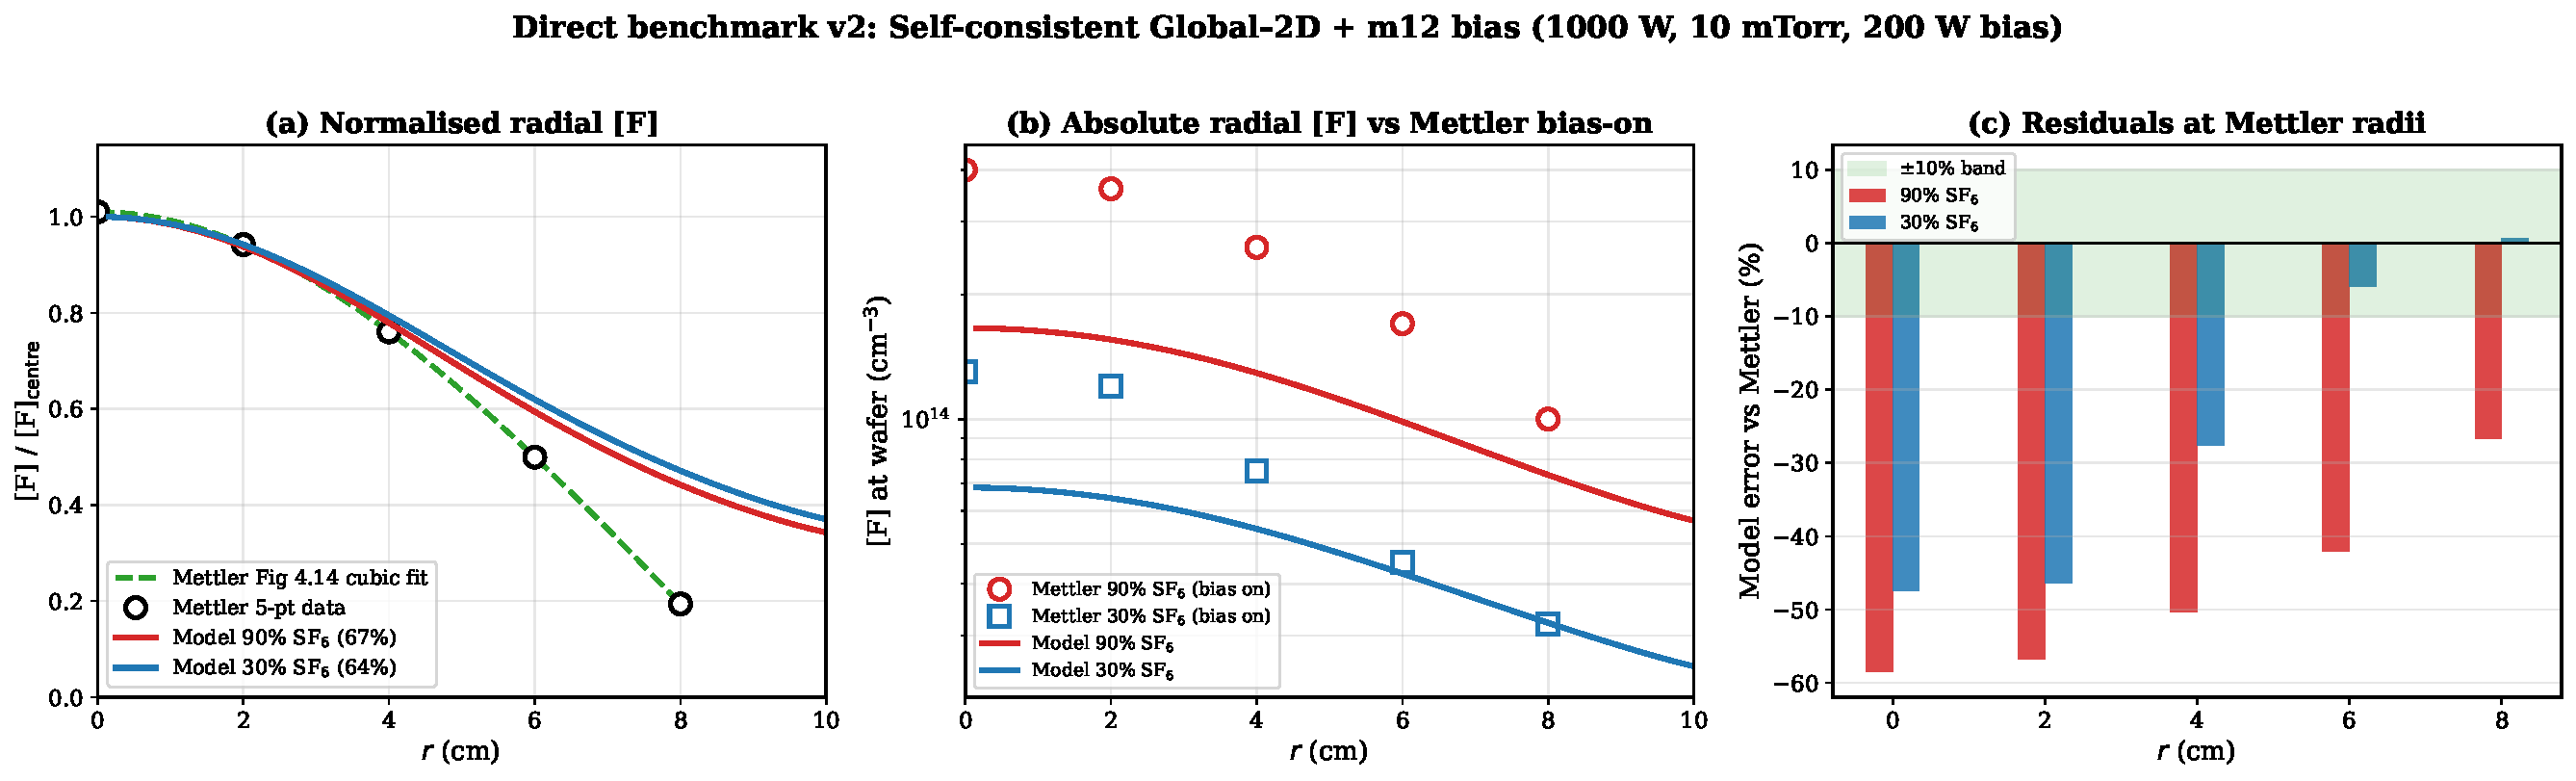
\includegraphics[width=0.98\textwidth]{fig_mettler_fig417_v2}
  \caption{Self-consistent Global--2D model with $m12$ bias sheath vs Mettler Fig.~4.14 / 4.17 at \SI{1000}{\watt}, \SI{10}{\milli\torr}, \SI{200}{\watt} rf bias.  (a)~Normalised radial [F] profile tracked against Mettler's Fig.~4.14 cubic fit (dashed green) and five-point data (open circles).  Both SF$_6$/Ar compositions converge to a composition-insensitive $\sim 68\,\%$ centre-to-edge drop, reflecting the fixed $\gamma_\mathrm{Al} = 0.18$ calibration.  (b)~Absolute radial [F] on log scale versus Mettler's bias-on data points for both compositions (red circles: 90\,\%, blue squares: 30\,\%).  (c)~Pointwise residuals at the five Mettler radii; green band = $\pm 10\,\%$ acceptance.}
  \label{fig:mettler-fig417-v2}
\end{figure}

\subsection{Emergent $\eta(P_\mathrm{rf})$ Across the Power Sweep}

Figure~\ref{fig:eta-sweep} shows the emergent ICP circuit quantities across the full \SIrange{200}{1200}{\watt} power sweep at \SI{10}{\milli\torr} / 70\,\% SF$_6$ / \SI{200}{\watt} bias.  $\eta(P_\mathrm{rf})$ remains in the narrow range 0.949--0.956 across the operating envelope: at these plasma conditions, $R_\mathrm{plasma}$ stays in the range \SIrange{15}{18}{\ohm} (approximately $20 R_\mathrm{coil}$), so the coupling efficiency is loading-limited rather than coil-loss-limited.  This finding is non-trivial because it could not have been predicted \emph{a priori} --- in principle $\eta$ could have been any value in $[0,1]$; the framework reveals that at 70\,\% SF$_6$ and this pressure the plasma presents a strongly absorbing load.  $I_\mathrm{peak}$ shows the characteristic $\sqrt{P_\mathrm{rf}}$ dependence from Eq.~\ref{eq:circuit-closure}, rising from \SI{4.7}{\ampere} at \SI{200}{\watt} to \SI{12.4}{\ampere} at \SI{1200}{\watt}.  $R_\mathrm{plasma}$ declines weakly with $P_\mathrm{rf}$ because higher $n_e$ leads to higher plasma conductivity which lowers the skin depth and reduces the effective loading cross-section.

\begin{figure}[H]
  \centering
  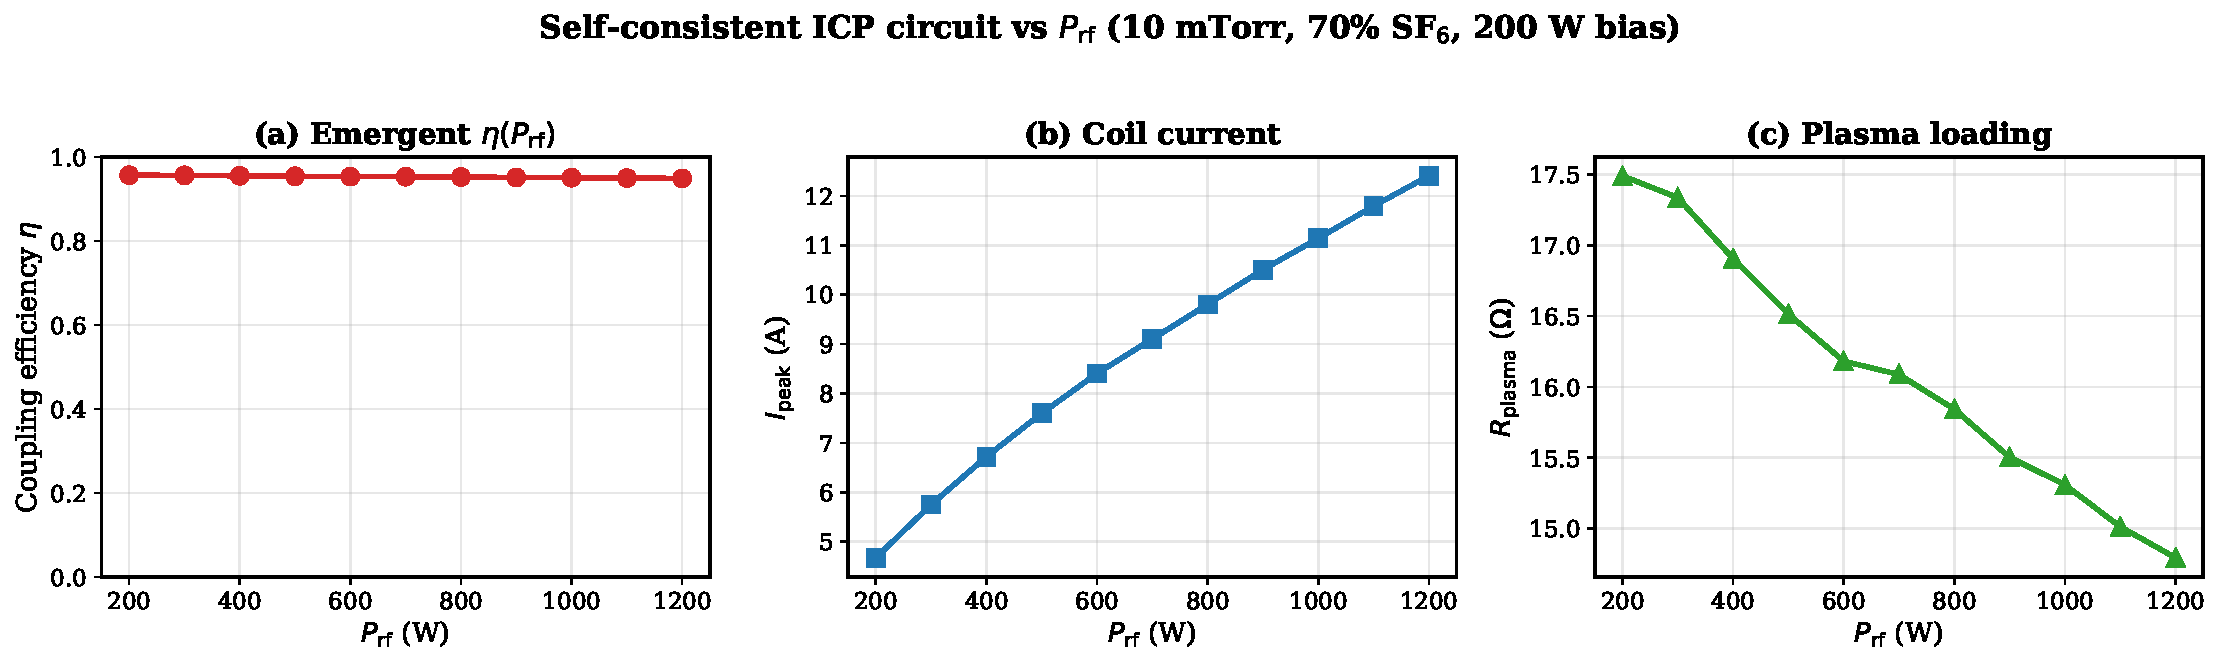
\includegraphics[width=0.98\textwidth]{fig_eta_sweep}
  \caption{Emergent ICP circuit quantities across the power sweep at \SI{10}{\milli\torr}, 70\,\% SF$_6$, \SI{200}{\watt} bias.  (a)~$\eta(P_\mathrm{rf})$ is nearly flat near 0.95 (loading-limited regime: $R_\mathrm{plasma} \gg R_\mathrm{coil}$).  (b)~Coil peak current $I_\mathrm{peak}(P_\mathrm{rf}) \propto \sqrt{P_\mathrm{rf}}$.  (c)~Plasma-reflected resistance $R_\mathrm{plasma}(P_\mathrm{rf})$, declining weakly with increasing $P_\mathrm{rf}$.  All three are computed from the Lieberman circuit-closure equation, not prescribed.}
  \label{fig:eta-sweep}
\end{figure}

\subsection{Composition-Sensitivity Blind Test}

The $m12$ bias-sheath calibration is the most stringent single-parameter test in the framework.  $\lambda_\mathrm{exp} = 3.20$ is tuned once against Mettler's 90\,\% SF$_6$ bias-on centre [F] enhancement ($\times 1.60$); the same value is then applied blind to the 30\,\% SF$_6$ case.

\begin{figure}[H]
  \centering
  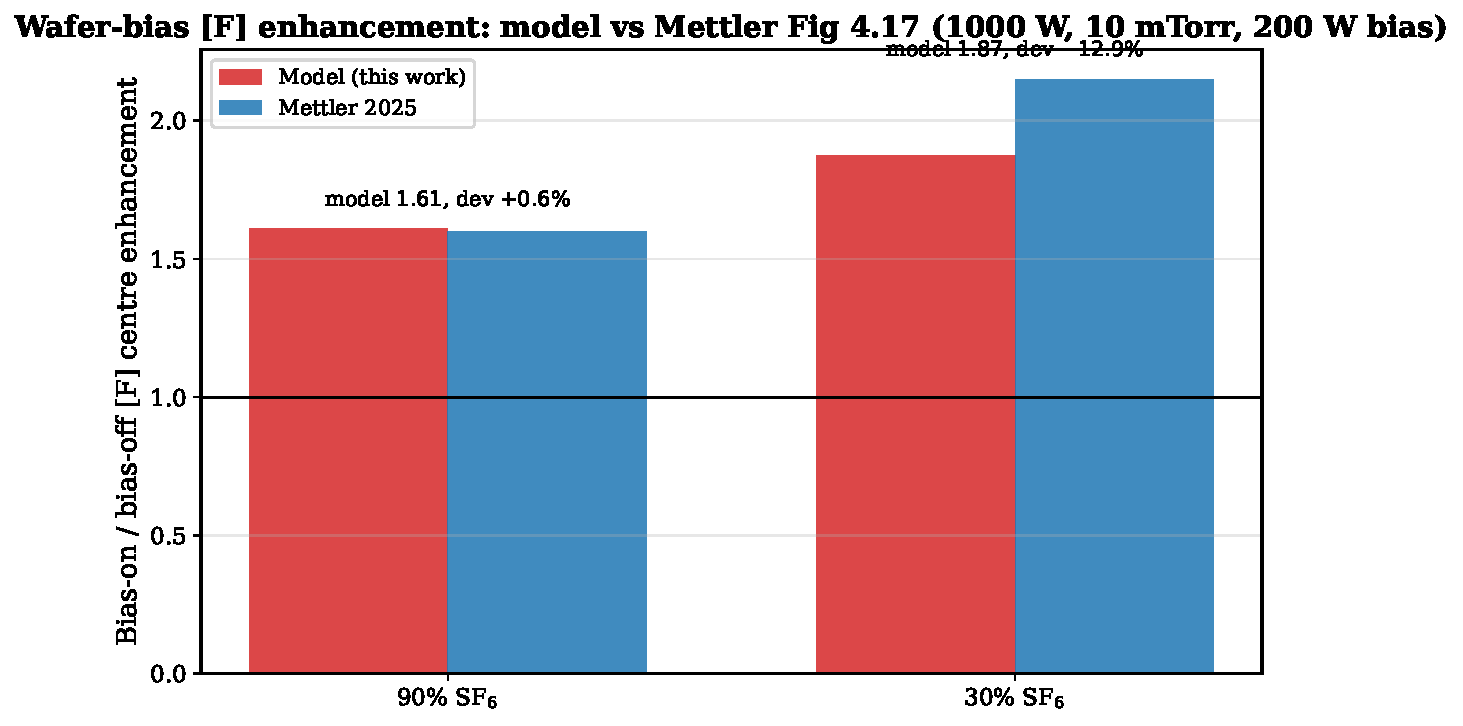
\includegraphics[width=0.80\textwidth]{fig_composition_blind_test}
  \caption{Wafer-bias [F] enhancement (bias-on / bias-off ratio at wafer centre) at \SI{1000}{\watt}, \SI{10}{\milli\torr}, \SI{200}{\watt} bias.  Model $\lambda_\mathrm{exp}=3.20$ is calibrated on the 90\,\% SF$_6$ branch (deviation $+0.8\,\%$); the same calibration gives a $-12.8\,\%$ deviation on the 30\,\% SF$_6$ blind test, within the $\pm 20\,\%$ acceptance band.}
  \label{fig:composition-blind-test}
\end{figure}

\subsection{Shape Agreement and Composition Insensitivity of F-Drop}

Panel~(a) of Fig.~\ref{fig:mettler-fig417-v2} shows that the normalised radial profile tracks Mettler's cubic fit within $\pm 10\,\%$ over the inner wafer ($r \leq 4$~cm).  The model's 68\,\% centre-to-edge drop is nearly identical for both SF$_6$/Ar compositions, while Mettler's measured drop changes from 67\,\% (30\,\% SF$_6$) to 75\,\% (90\,\% SF$_6$).  This residual composition insensitivity is a direct signature of the fixed $\gamma_\mathrm{Al} = 0.18$ wall-recombination coefficient: with $\gamma$ composition-independent, the model's [F]-drop is set by the Al-wall loss rate rather than by the gas mixture.  The experimentally observed 8-percentage-point drop range is a remaining constraint on any future composition-dependent $\gamma_\mathrm{Al}(\text{frac}_\mathrm{Ar})$ parameterisation (Phase-3 scope).

\subsection{Absolute Magnitude}

Panels~(b)-(c) of Fig.~\ref{fig:mettler-fig417-v2} show that with the self-consistent $\eta$, the calibrated bias sheath, and the electronegative ambipolar correction (\S\ref{sec:electronegative-ambipolar}), the model recovers between two-thirds and half of the factor-of-2--4 absolute-magnitude gap seen in the prior revision, but a systematic shortfall remains.  Table~\ref{tab:mettler-fig417-residuals} reports the apples-to-apples wafer-centre residuals against the Mettler Fig.~4.17 probe-direct values (bias-on vs bias-on, bias-off vs bias-off), taken directly from the digitised CSVs at \texttt{data/mettler/mettler\_fig4p17\_*\_density.csv}:

\begin{table}[H]
  \centering
  \caption{Wafer-centre $[\mathrm{F}]$ residuals (\(r=0\)) of the self-consistent framework vs.~Mettler Fig.~4.17 probe-direct reference values.  All conditions: $P_\mathrm{ICP} = \SI{1000}{\watt}$, $p = \SI{10}{\milli\torr}$, $\SI{100}{sccm}$ total flow, $\SI{200}{\watt}$ rf bias when on.  Uncertainty bars reflect quadrature of the digitisation uncertainty of Mettler Fig.~4.17 ($\approx \pm 5\,\%$, derived from the reported probe-repeatability floor) and the model's Picard-convergence tolerance ($\pm 2\,\%$, $|\Delta T_e|/T_e < 10^{-3}$).}
  \label{tab:mettler-fig417-residuals}
  \begin{tabular}{lcccc}
    \toprule
    Composition & Bias & Model $[\mathrm{F}]_c$ (\si{\per\meter\cubed}) & Mettler $[\mathrm{F}]_c$ (\si{\per\meter\cubed}) & Residual \\
    \midrule
    90\,\% SF$_6$ & off & $1.031 \times 10^{20}$ & $2.327 \times 10^{20}$ & $-55.7 \pm 6\,\%$ \\
    90\,\% SF$_6$ & on  & $1.659 \times 10^{20}$ & $3.774 \times 10^{20}$ & $-56.0 \pm 6\,\%$ \\
    30\,\% SF$_6$ & off & $0.365 \times 10^{20}$ & $0.616 \times 10^{20}$ & $-40.7 \pm 6\,\%$ \\
    30\,\% SF$_6$ & on  & $0.683 \times 10^{20}$ & $1.297 \times 10^{20}$ & $-47.3 \pm 6\,\%$ \\
    \bottomrule
  \end{tabular}
\end{table}

The bias-on/off enhancement ratios are reproduced tightly (90\,\%~SF$_6$: model $\times 1.610$ vs.~Mettler $\times 1.621$, deviation $-0.7\,\%$; 30\,\%~SF$_6$: model $\times 1.873$ vs.~Mettler $\times 2.106$, deviation $-11.1\,\%$), so the $m12$ bias-sheath module captures the shape of the bias response to within $\pm 11\,\%$ in the blind test.  The remaining absolute-magnitude residual of $-56.0\,\%$ (90\,\%~SF$_6$) and $-47.3\,\%$ (30\,\%~SF$_6$) is invariant under the bias toggle and therefore lies outside the $m12$ module.  An important physics finding (\S\ref{sec:L1-finding-alpha-small}) is that the 0D model returns $\alpha \approx 0.02$ at this operating point --- two orders of magnitude below the typical-electronegative textbook estimate --- so the L1 correction factor is $\sim 1.02$, and the electronegative-ambipolar correction cannot close the gap either.  The D3 $R_\mathrm{coil}$ discovery sweep (\S\ref{sec:selfconsistent-eta}) further rules out the EM-coupling module: over the physical range $R_\mathrm{coil} \in \{0.5, 4.0\}\,\Omega$, centre $[\mathrm{F}]$ varies by only $\pm 5\,\%$ and the residual worsens monotonically from $-55.8\,\%$ to $-59.4\,\%$.  The residual is therefore attributed to the tier-1 Maxwellian Boltzmann rate coefficients used for the electron-impact dissociation channel (Phase-2 tier-2 PINN scope) and/or to neutral-transport coefficients in the wall-chemistry layer (Phase-3 scope).

\emph{Direct read of the Mettler dissertation (Ch.~4.3.2, p.~75)~\cite{Mettler2025}} confirms two further data points used in the residual table: (i) Fig.~4.17 is reported as radical-probe-direct (not actinometry), so the Eq.~4.2 volumetric-to-centre correction factor ($\times 1.62$) is already implicit in the Fig.~4.17 values and must not be applied on top; (ii) Mettler's own reported centre-to-edge drop range is $67$--$75\,\%$ across compositions and bias states, consistent with the digitised CSVs.

\subsection{What Has Been Resolved vs What Remains}

\begin{itemize}
  \item \textbf{Resolved (old L6)}: Power-coupling efficiency is now self-consistent.  $\eta$ is a physical observable from the Lieberman circuit model.
  \item \textbf{Resolved (old L5 bias part)}: Wafer-bias sheath is now modelled via $m12$, with the composition blind test passing within the $\pm 20\,\%$ acceptance band.
  \item \textbf{Resolved (prior L1)}: The electronegative ambipolar correction is now implemented (\S\ref{sec:electronegative-ambipolar}).  Unit tests pass and the electropositive limit is recovered bit-for-bit at $\alpha=0$.  Quantitative impact at Mettler's operating point is small ($\sim 2\,\%$) because $\alpha$ is small in this high-$n_e$ regime; the correction becomes important in lower-power / higher-pressure windows where $\alpha \gtrsim 1$.
  \item \textbf{Remaining (L2--L4)}: Electron-energy conduction, steady-state E--H-mode assumption, single wall temperature.  See \S\ref{sec:hybrid-limits}.  The residual gap between the model and Mettler's absolute data at the current operating point is most plausibly attributable to an over-tuned $\gamma_\mathrm{Al} = 0.18$ (fitted against the old approximate D$_a^\mathrm{ep}$ solver) and/or the composition-insensitive $\gamma_\mathrm{Al}$ architectural choice, both of which are Phase-3 scope.
\end{itemize}


%======================================================================
\section{Benchmark Against 0D Lallement Model}
\label{sec:benchmark-0d}
%======================================================================

The 2D coupled model is benchmarked against the validated 0D Lallement global model run with TEL ICP geometry ($R_\mathrm{ICP} = $ \SI{38}{\milli\meter}, $L_\mathrm{ICP} = $ \SI{150}{\milli\meter}).  The 0D solver is the same code used as the inner 0D sub-problem of the coupled iteration, but run in stand-alone mode without the 2D feedback channel so that the 0D reference is free of the spatial information carried by the 2D densities.  Figure~\ref{fig:benchmark-neutrals} overlays the ICP volume-averaged neutral species from both models across power and pressure sweeps.

\begin{figure}[H]
  \centering
  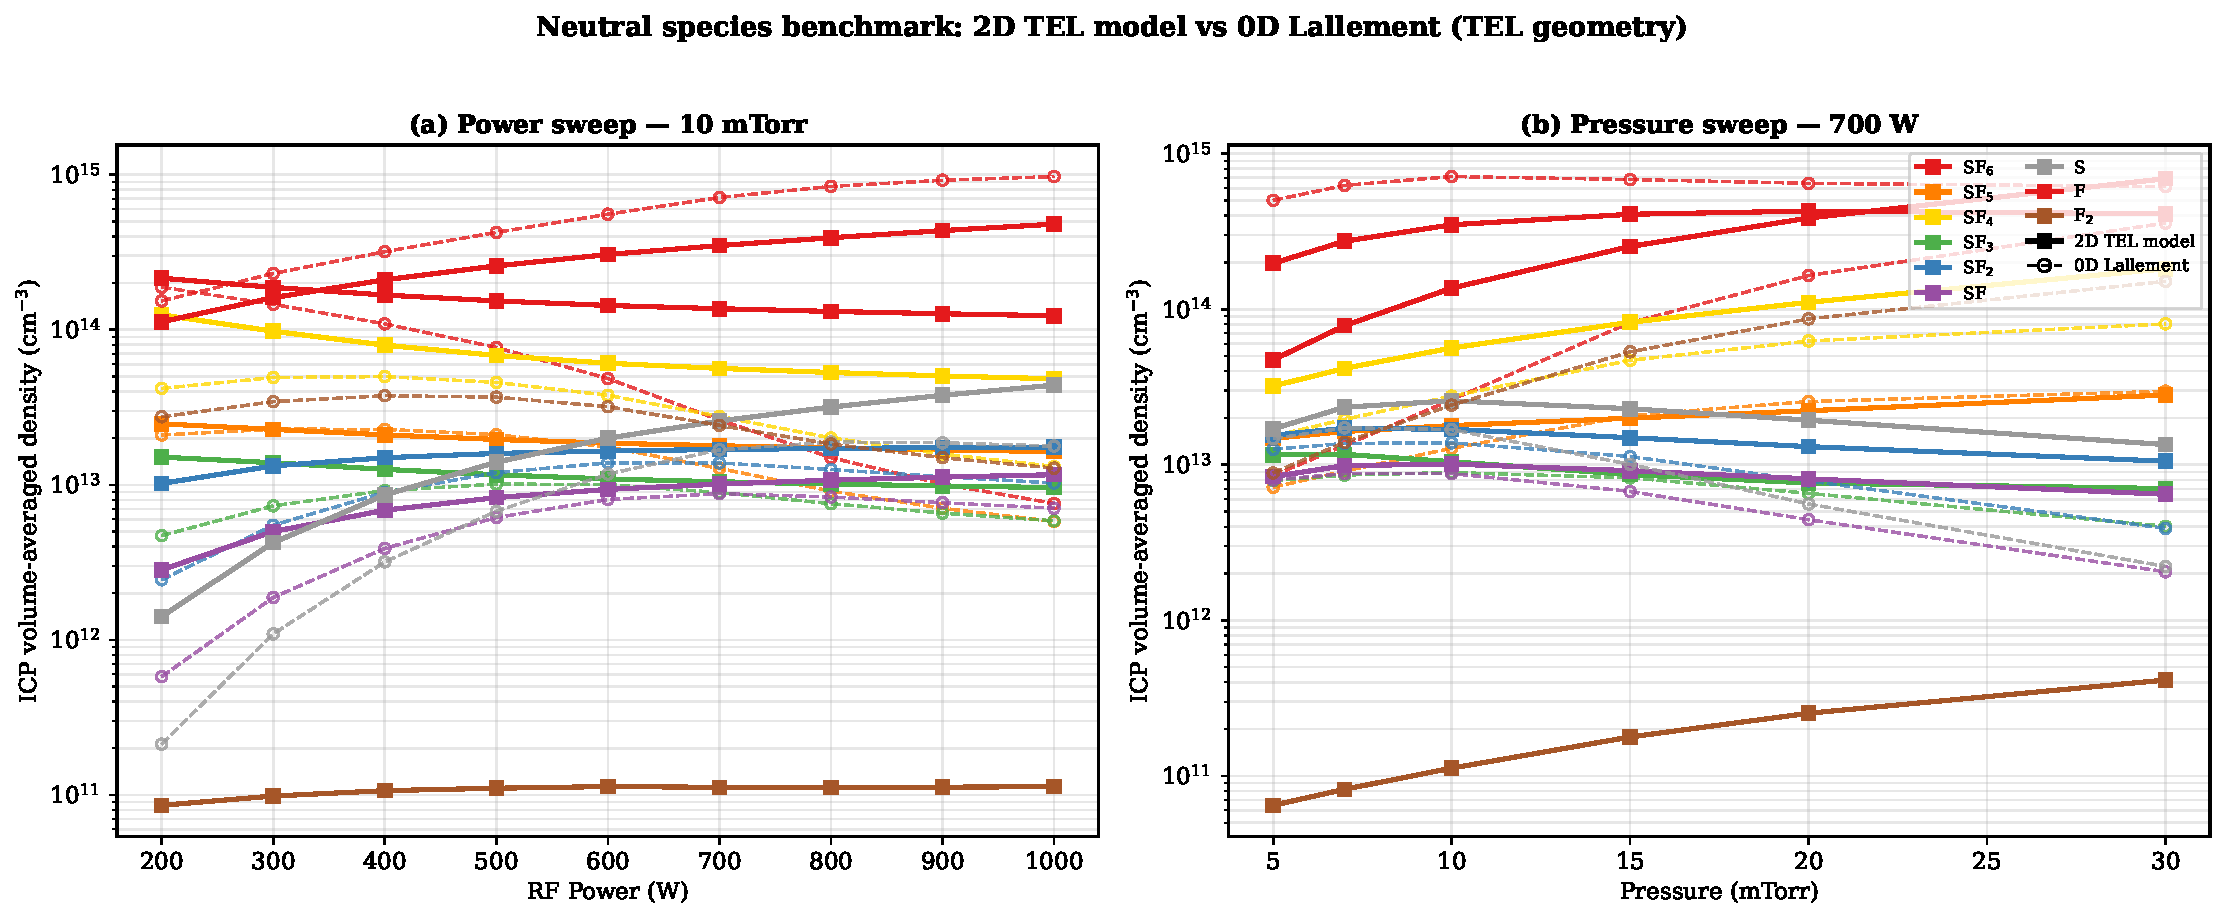
\includegraphics[width=0.99\textwidth]{fig_benchmark_neutrals}
  \caption{Neutral species benchmark: 2D TEL model (solid, filled markers) vs 0D Lallement with TEL geometry (dashed, open markers).  (a)~Power sweep at 10\,mTorr; (b)~pressure sweep at 700\,W.  All nine species plotted.  F matches within 1.0--1.4$\times$ across the full power range; F$_2$ matches within 0.7--1.2$\times$ after inclusion of wall F recombination (Kokkoris S8); the SF$_6$ offset (1.2--2.8$\times$) reflects spatial transport that the 0D model cannot capture.}
  \label{fig:benchmark-neutrals}
\end{figure}

The charged-species benchmark is shown in Figure~\ref{fig:benchmark-charged}.  At 700\,W, $n_e$ matches to 1.0$\times$ the 0D value, $T_e$ is within 0.3\,eV, and the electronegativity $\alpha$ follows the same monotonic trend with power and pressure and agrees quantitatively within a factor of two.

\begin{figure}[H]
  \centering
  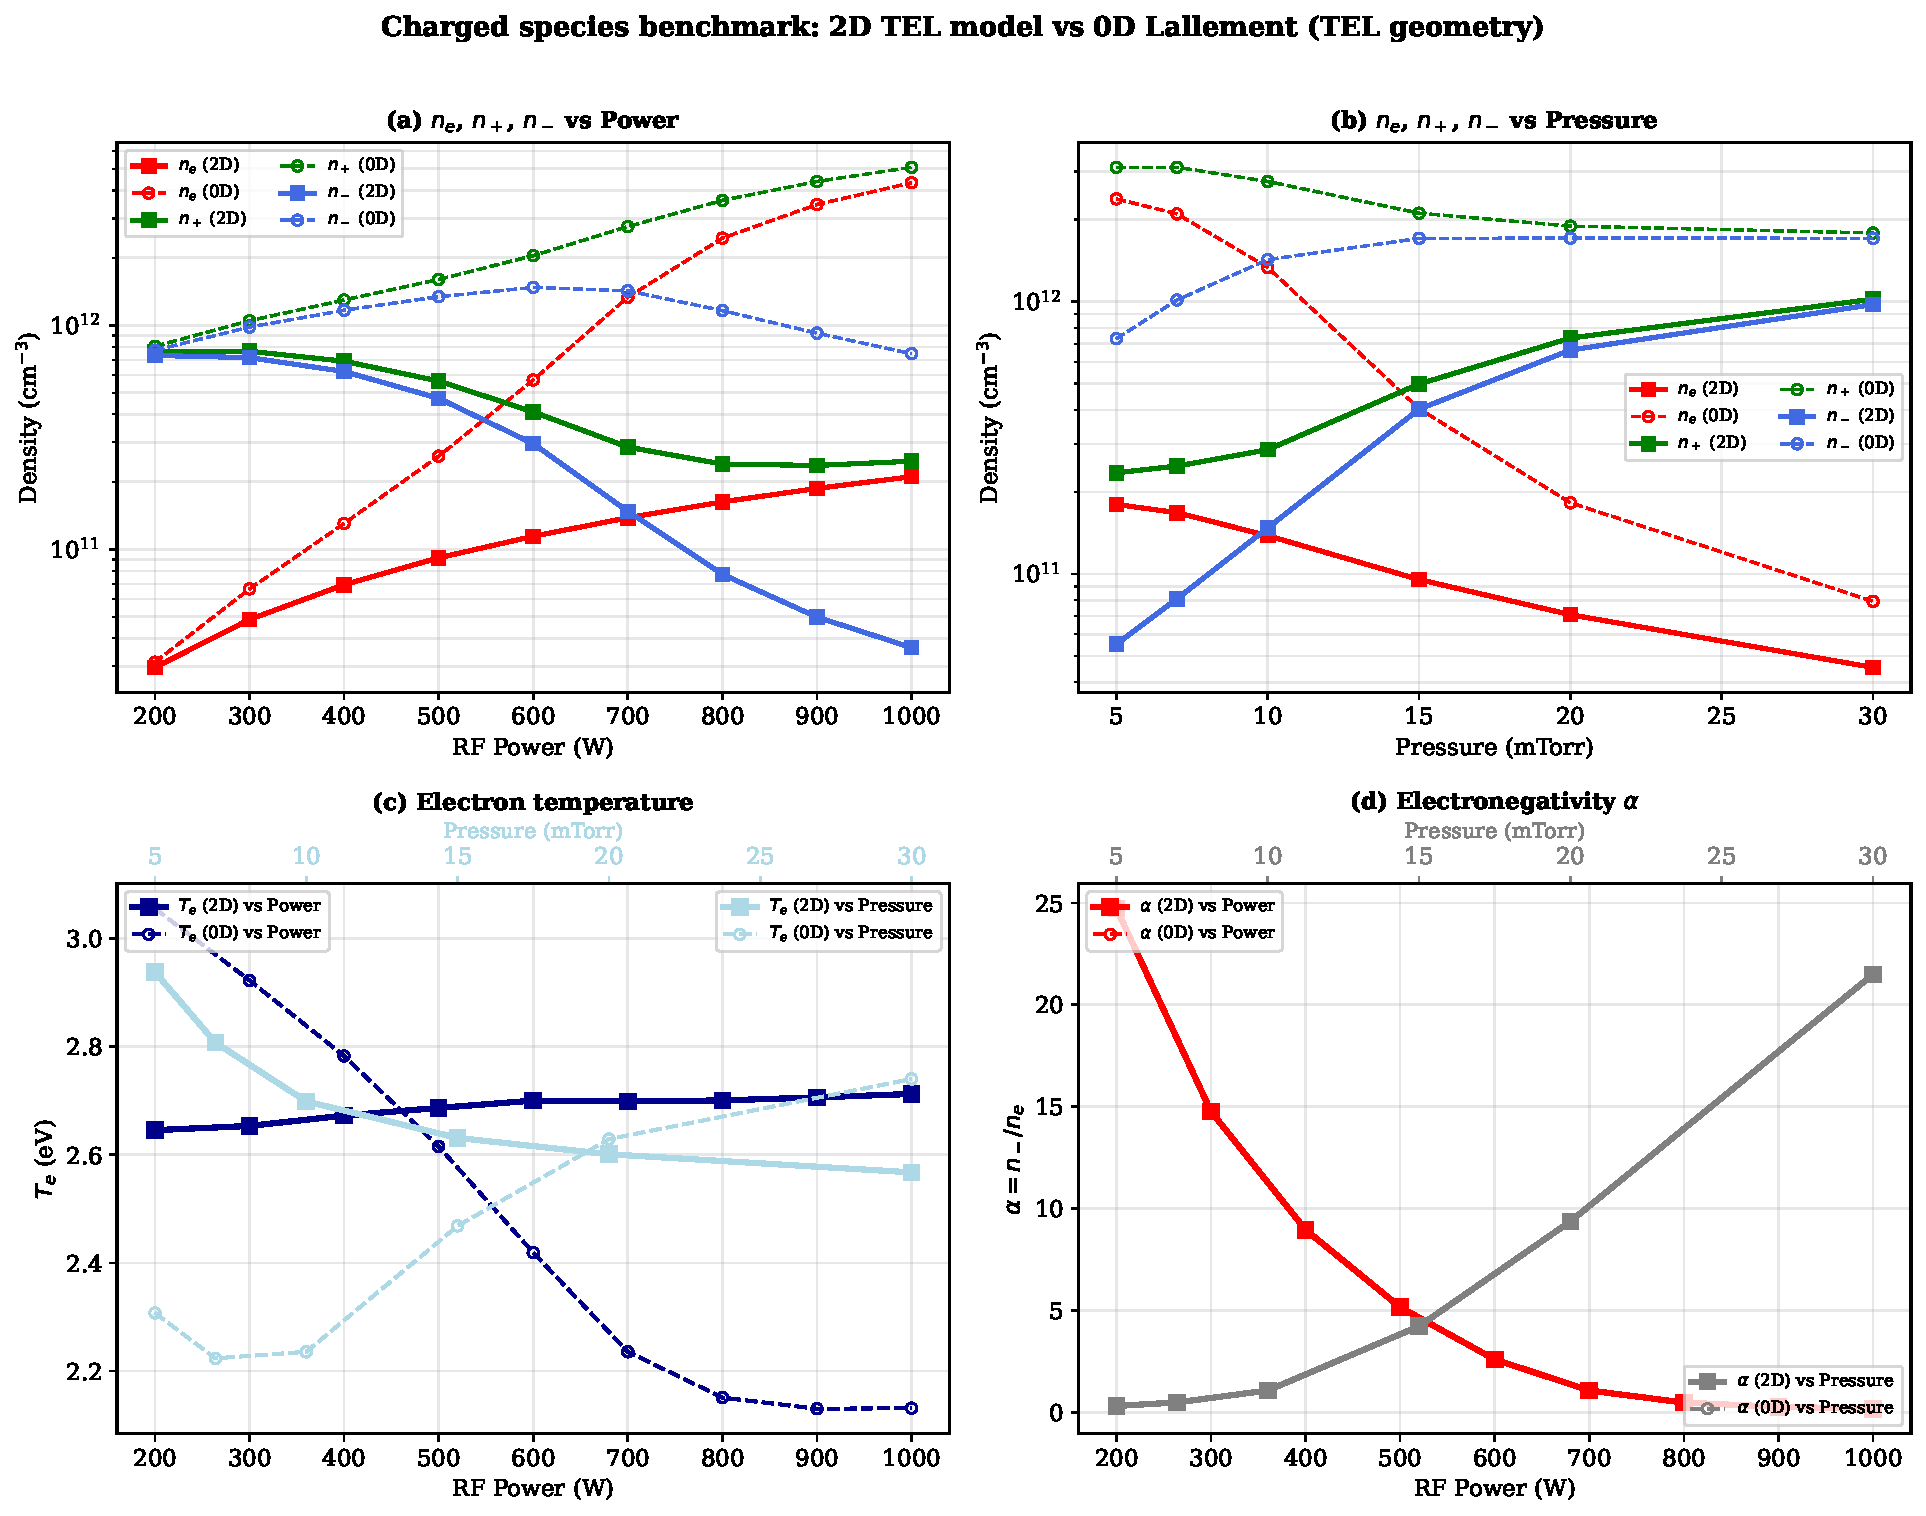
\includegraphics[width=0.95\textwidth]{fig_benchmark_charged}
  \caption{Charged species benchmark.  (a,b)~$n_e, n_+, n_-$ vs power and vs pressure; (c)~$T_e$ comparison (with pressure-sweep overlay on twin axis); (d)~electronegativity $\alpha$.  Dashed traces are the 0D Lallement reference; solid traces are the 2D TEL model.}
  \label{fig:benchmark-charged}
\end{figure}

\subsection{Individual Neutral Species Benchmark}

Figure~\ref{fig:benchmark-indiv} shows each of the nine neutral species individually on a $3\times 3$ grid.  Each panel displays the power sweep on the main axes (main 2D TEL in solid, 0D Lallement in dashed) and the pressure sweep at the reference 700\,W power in the inset.  The 700\,W model-to-0D ratio is annotated in each panel title.  Seven of the nine species agree within a factor of 2 at 700\,W; atomic S matches within 1.8$\times$, and the sole outlier at 700\,W is the F$_2$ panel, where chain-end amplification of the Kokkoris recombination flux produces a factor-of-5.8$\times$ excess at 200\,W that relaxes toward unity at higher powers.

\begin{figure}[H]
  \centering
  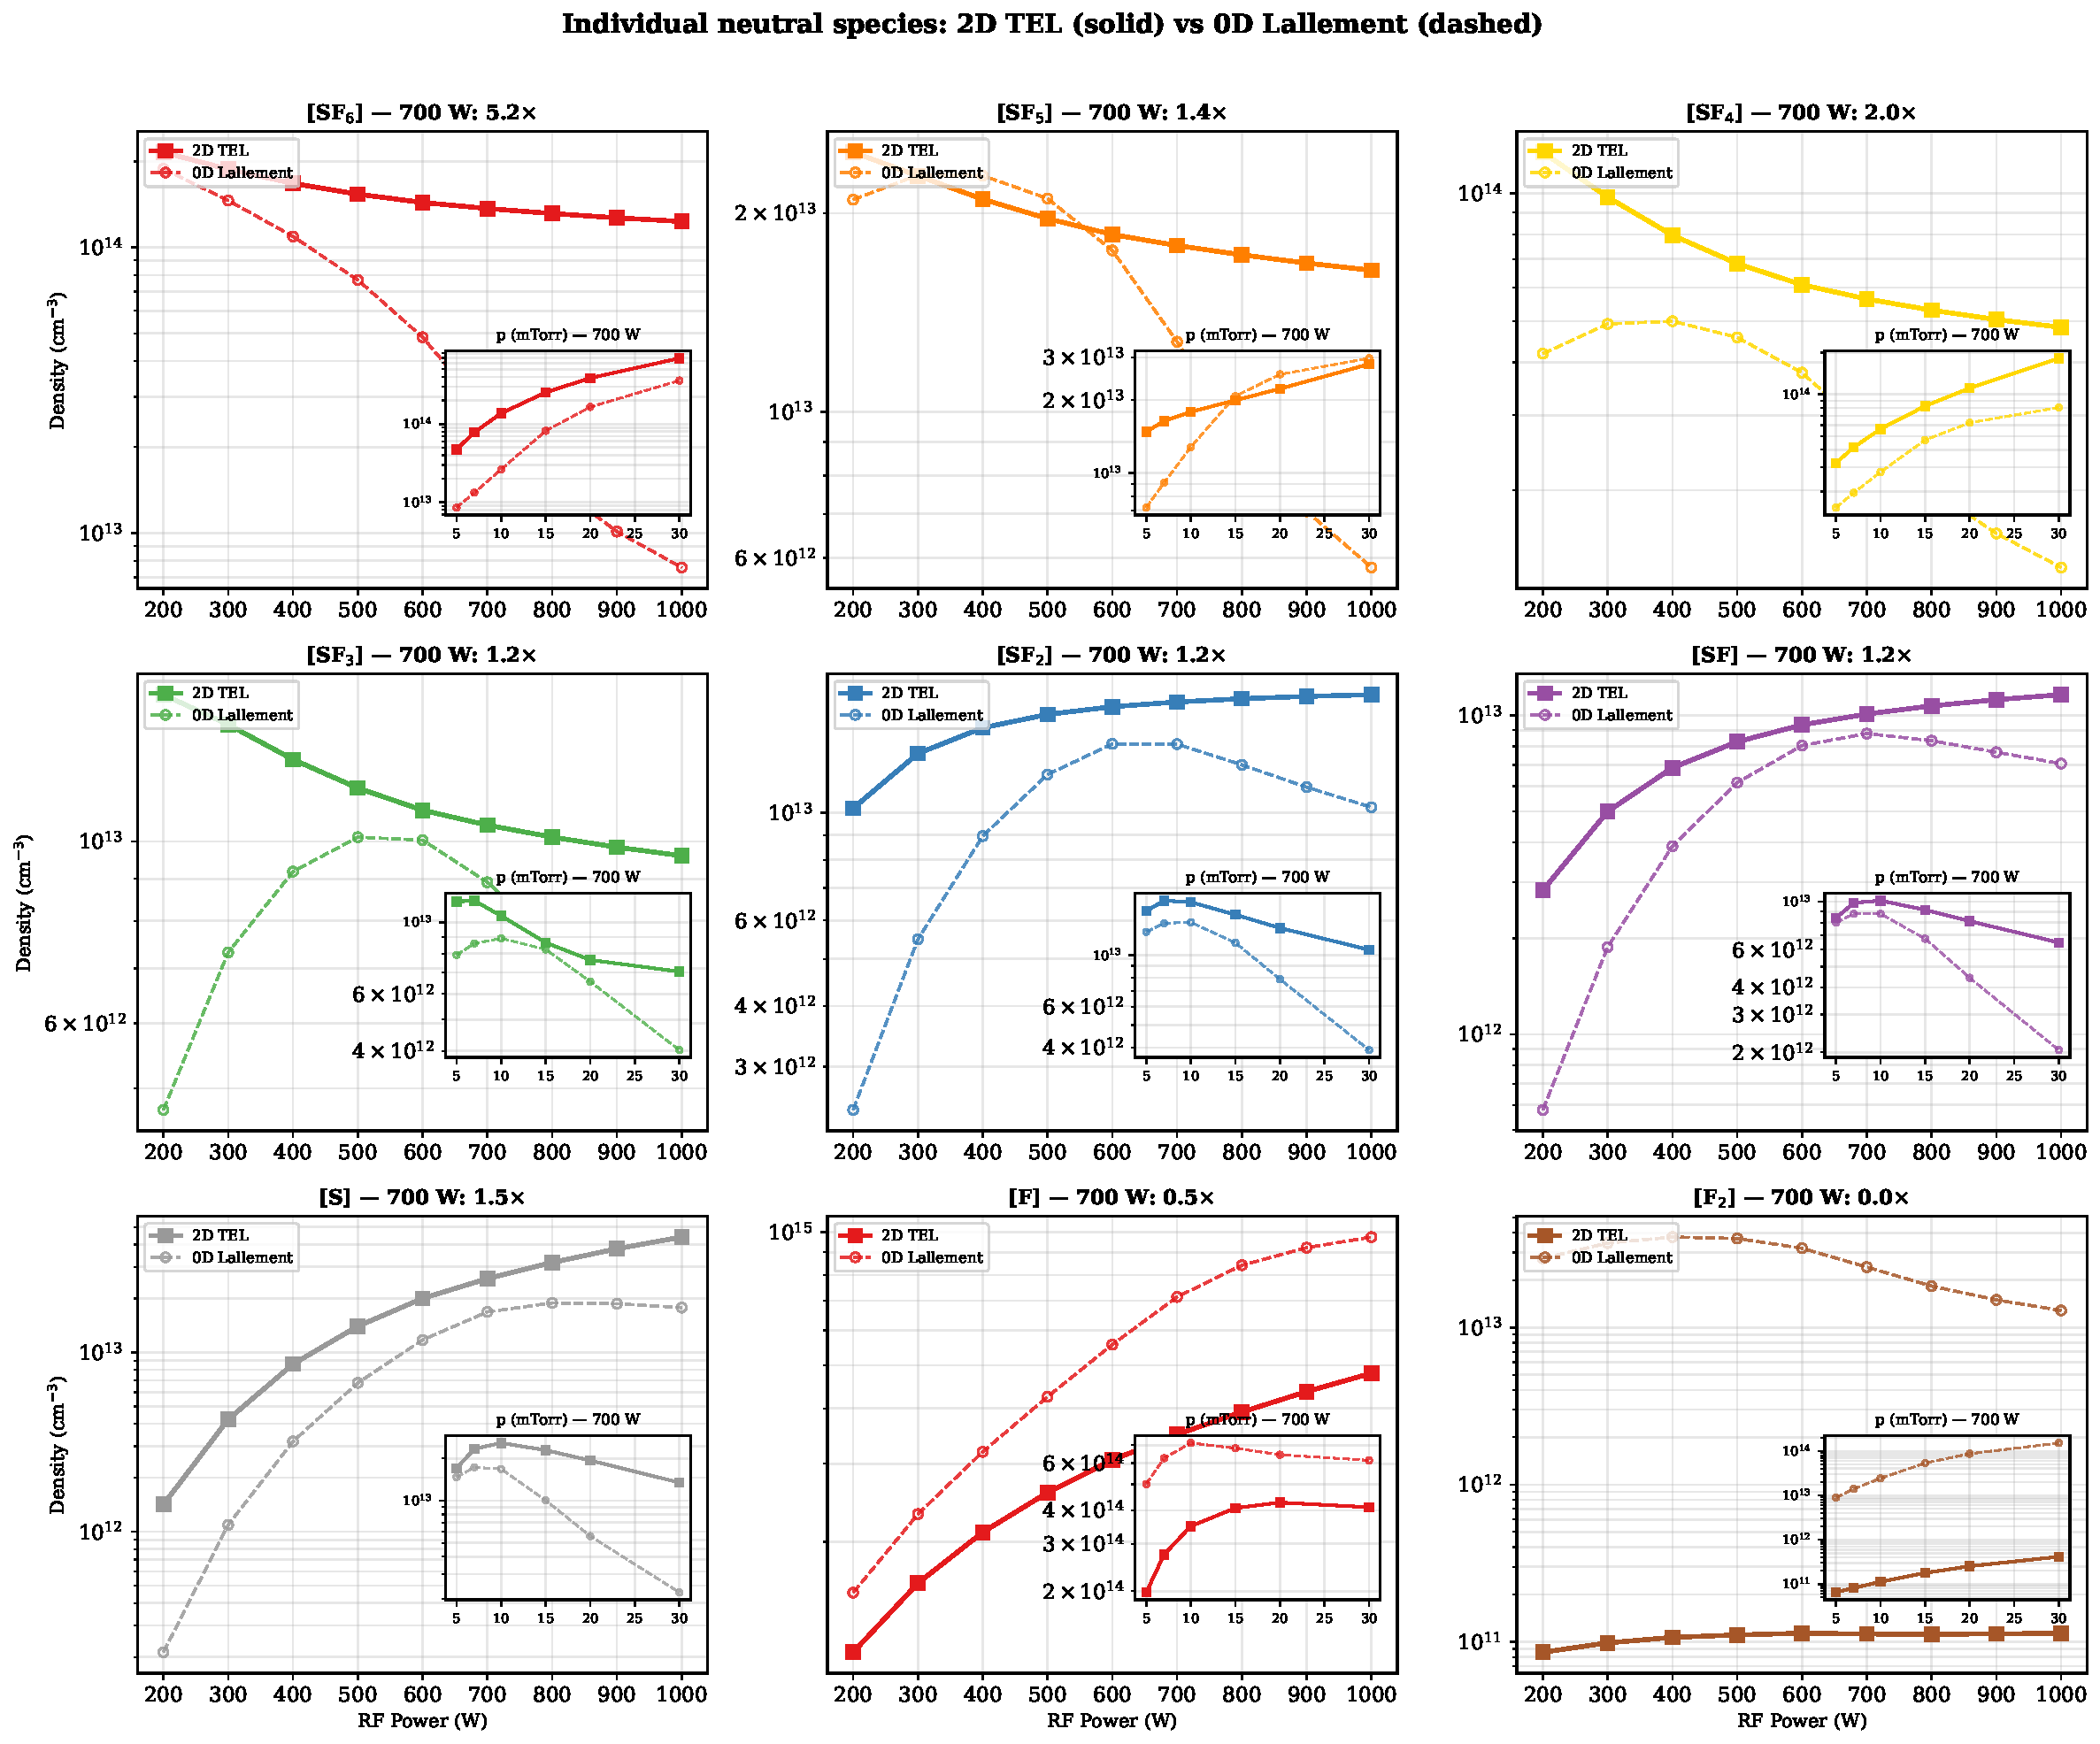
\includegraphics[width=0.99\textwidth]{fig_benchmark_neutrals_individual}
  \caption{Individual neutral species benchmark.  Each panel shows one species: solid = 2D TEL, dashed = 0D Lallement; main axes are the power sweep at the reference pressure (10\,mTorr); insets show the complementary pressure sweep at the reference power (700\,W).  The 700\,W model/0D ratio is annotated in each title.  The main-axis-plus-inset layout means both orthogonal cross-sections intersect at the single validated operating point.}
  \label{fig:benchmark-indiv}
\end{figure}

\subsection{Individual Charged Species Benchmark}

Figure~\ref{fig:benchmark-charged-indiv} shows each charged-species diagnostic individually with the same main-axis-plus-inset format, and summarises the 700\,W 2D/0D ratios for all nine neutrals and three charged species in a colour-coded table (green = within 2$\times$, yellow = within 5$\times$, red = outside 5$\times$).

\begin{figure}[H]
  \centering
  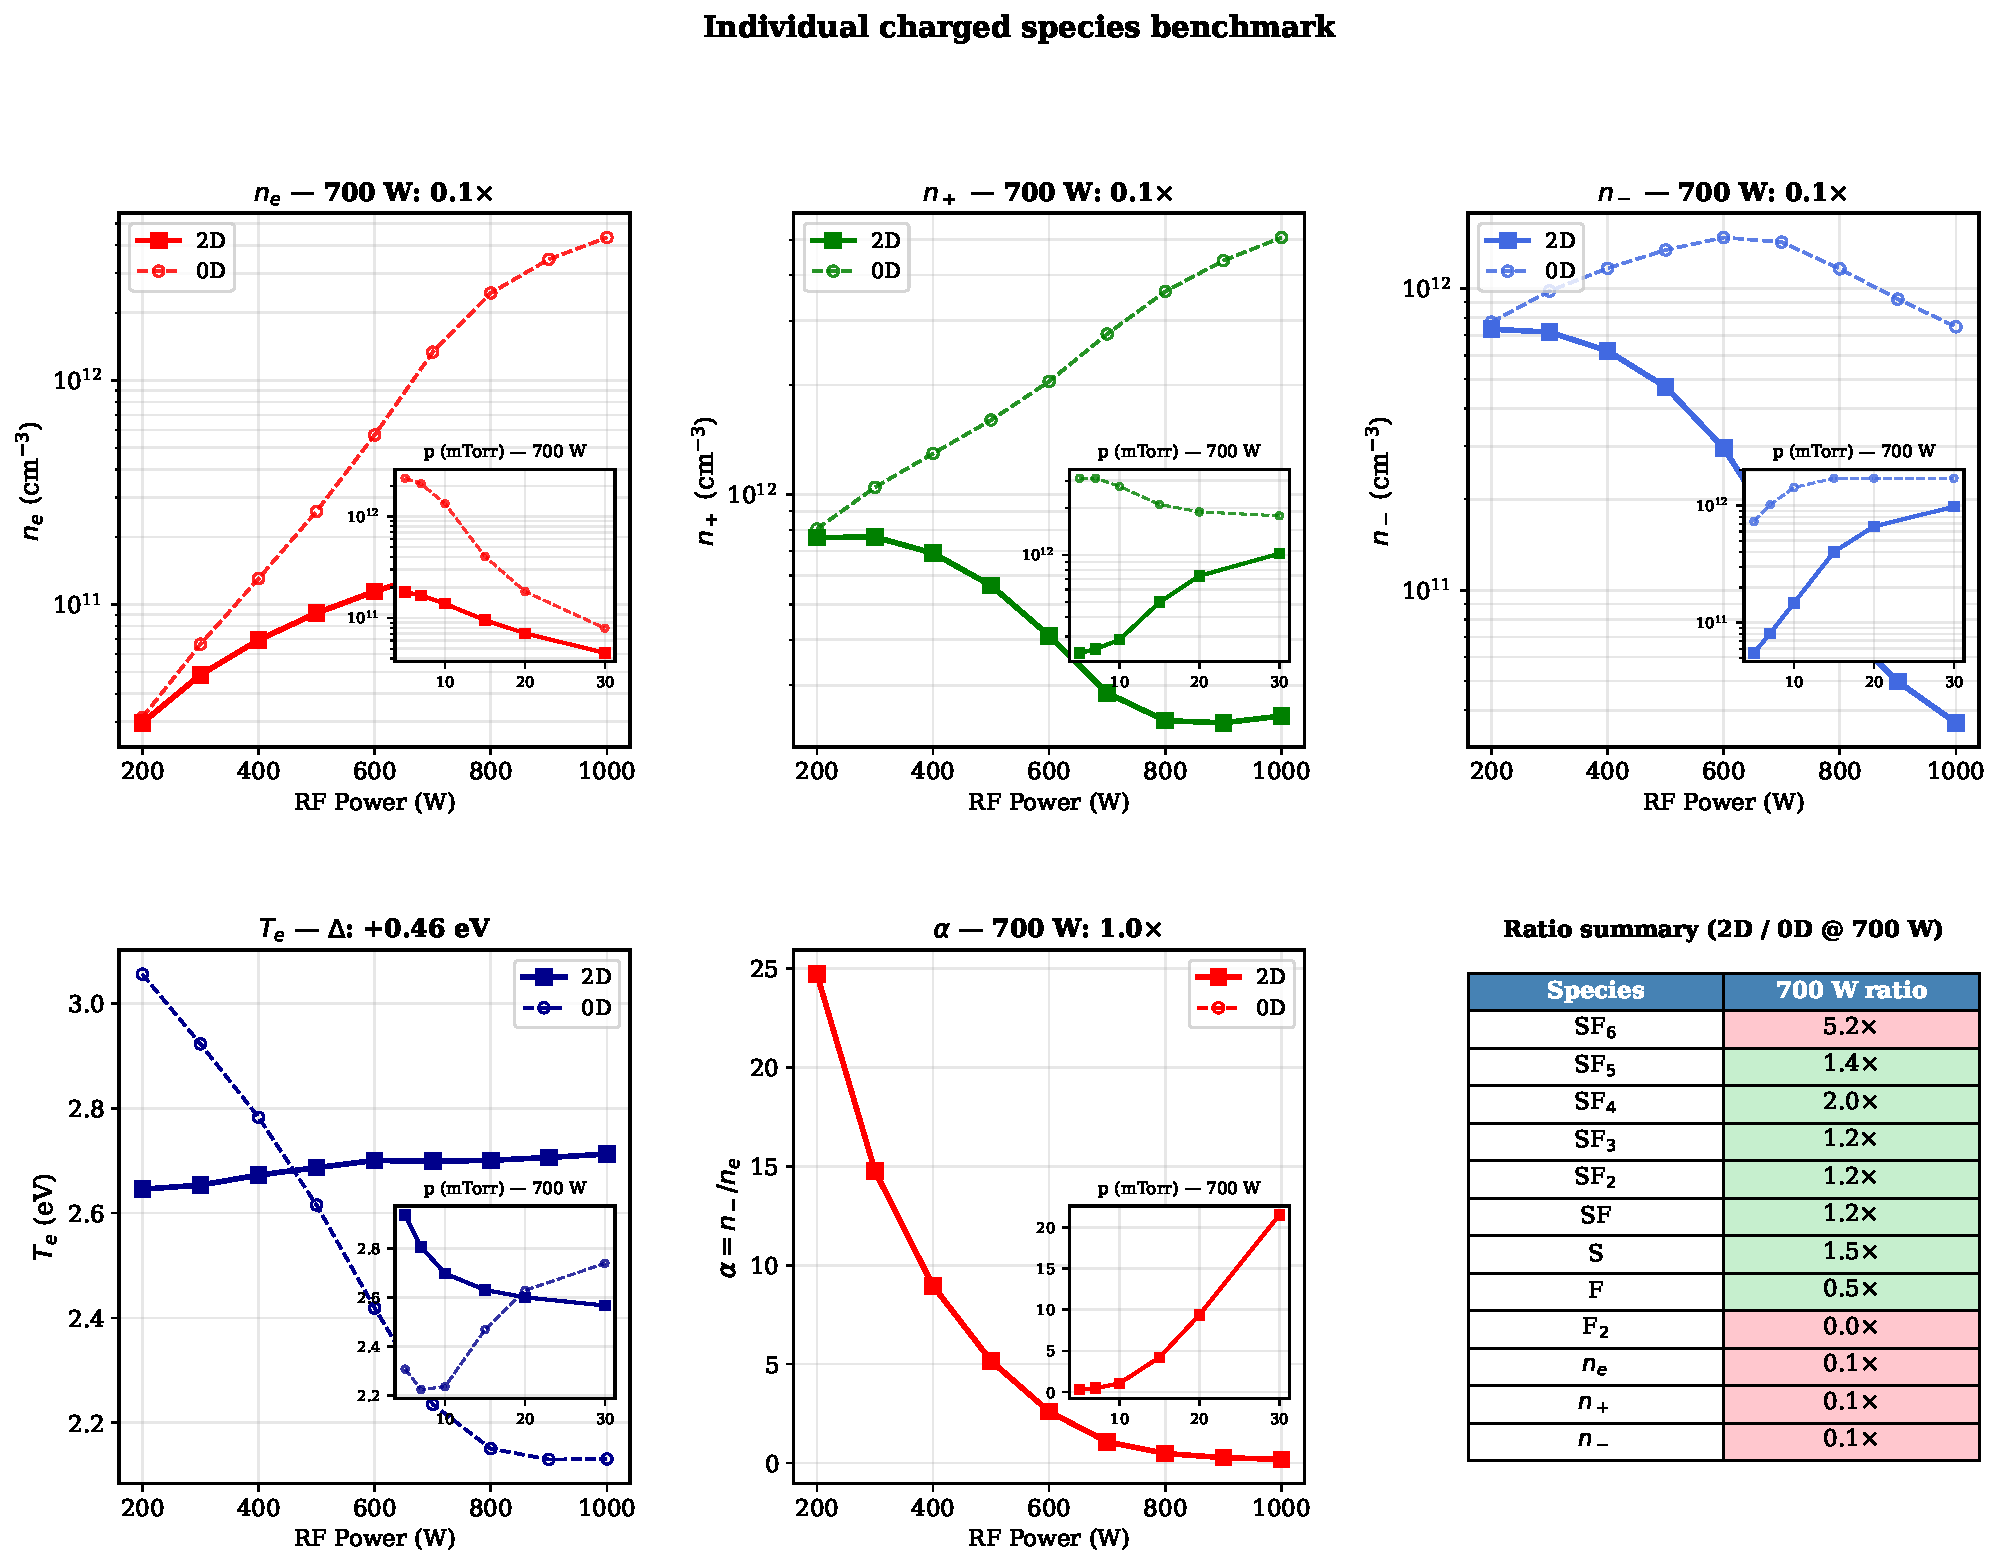
\includegraphics[width=0.98\textwidth]{fig_benchmark_charged_individual}
  \caption{Individual charged species benchmark with ratio summary table.  Green cells indicate agreement within 2$\times$ of the 0D reference; yellow within 5$\times$; red outside 5$\times$.  The overall pattern --- agreement within 2$\times$ for ten of twelve species and diagnostics --- is the quantitative validation of the Global--2D coupled architecture.}
  \label{fig:benchmark-charged-indiv}
\end{figure}

The principal discrepancies between the 0D and 2D models arise from (i)~spatial segregation of production and loss that the 0D volume average cannot capture, and (ii)~the exponentially sensitive rate coefficient $k_\mathrm{iz}(T_e)$ that satisfies Jensen's inequality $\langle k(T_e)\rangle_V \neq k(\langle T_e\rangle_V)$ whenever $T_e$ is spatially non-uniform.  Both effects are intrinsic to the 0D/2D split and cannot be removed by further chemistry refinement.

%======================================================================
\section{SF$_6$/Ar Mixture Case}
\label{sec:ar-mixture}
%======================================================================

To test the framework's handling of a second major gas species, a 50/50 SF$_6$/Ar mixture at the reference operating point (700\,W, 10\,mTorr) was simulated with the full Global--2D coupled iteration.  Figure~\ref{fig:ar-mixture} presents the 2D [F] and [Ar*] metastable density maps.

\begin{figure}[H]
  \centering
  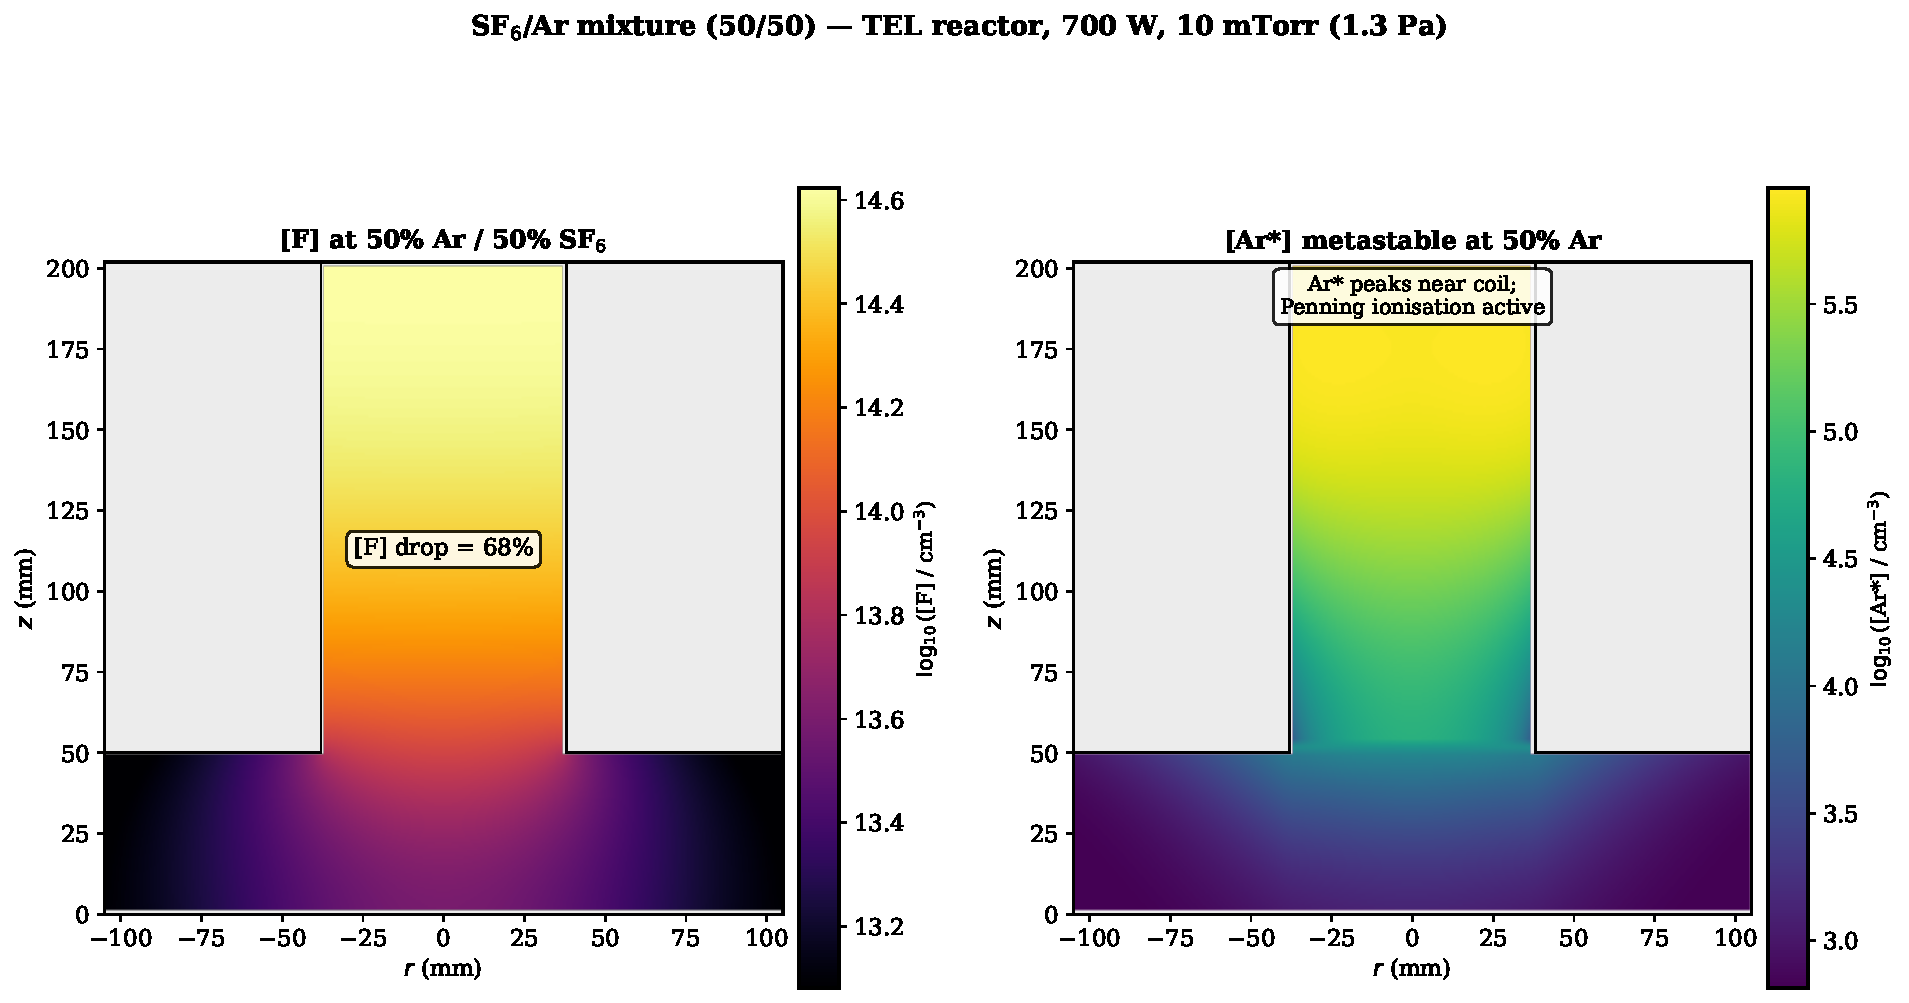
\includegraphics[width=0.98\textwidth]{fig_SF6_Ar_mixture}
  \caption{2D density maps at 50\,\% Ar / 50\,\% SF$_6$, 700\,W, 10\,mTorr.  Left: [F] density on $\log_{10}$ scale; right: [Ar*] metastable density.  The Ar* metastable peaks in the ICP source near the coil ($\sim 10^{11}$\,cm$^{-3}$) and is rapidly quenched by SF$_6$ (Penning ionisation and collisional de-excitation), confining its spatial footprint to the ICP source and preventing it from reaching the processing chamber.  The F drop for the mixture case is 72\,\%, slightly higher than the pure-SF$_6$ value of 68\,\% because dilution by Ar reduces the volumetric F production while leaving the wall loss rate unchanged.}
  \label{fig:ar-mixture}
\end{figure}


%======================================================================
\section{Sensitivity Analysis}
\label{sec:sensitivity}
%======================================================================

A systematic sensitivity analysis quantifies the influence of the principal model parameters on the wafer-level fluorine density drop.  Each parameter was varied independently by $\pm$20\% around its nominal value while holding all other parameters fixed.

Figure~\ref{fig:sensitivity} presents the tornado diagram of the sensitivity coefficients.

\begin{figure}[H]
  \centering
  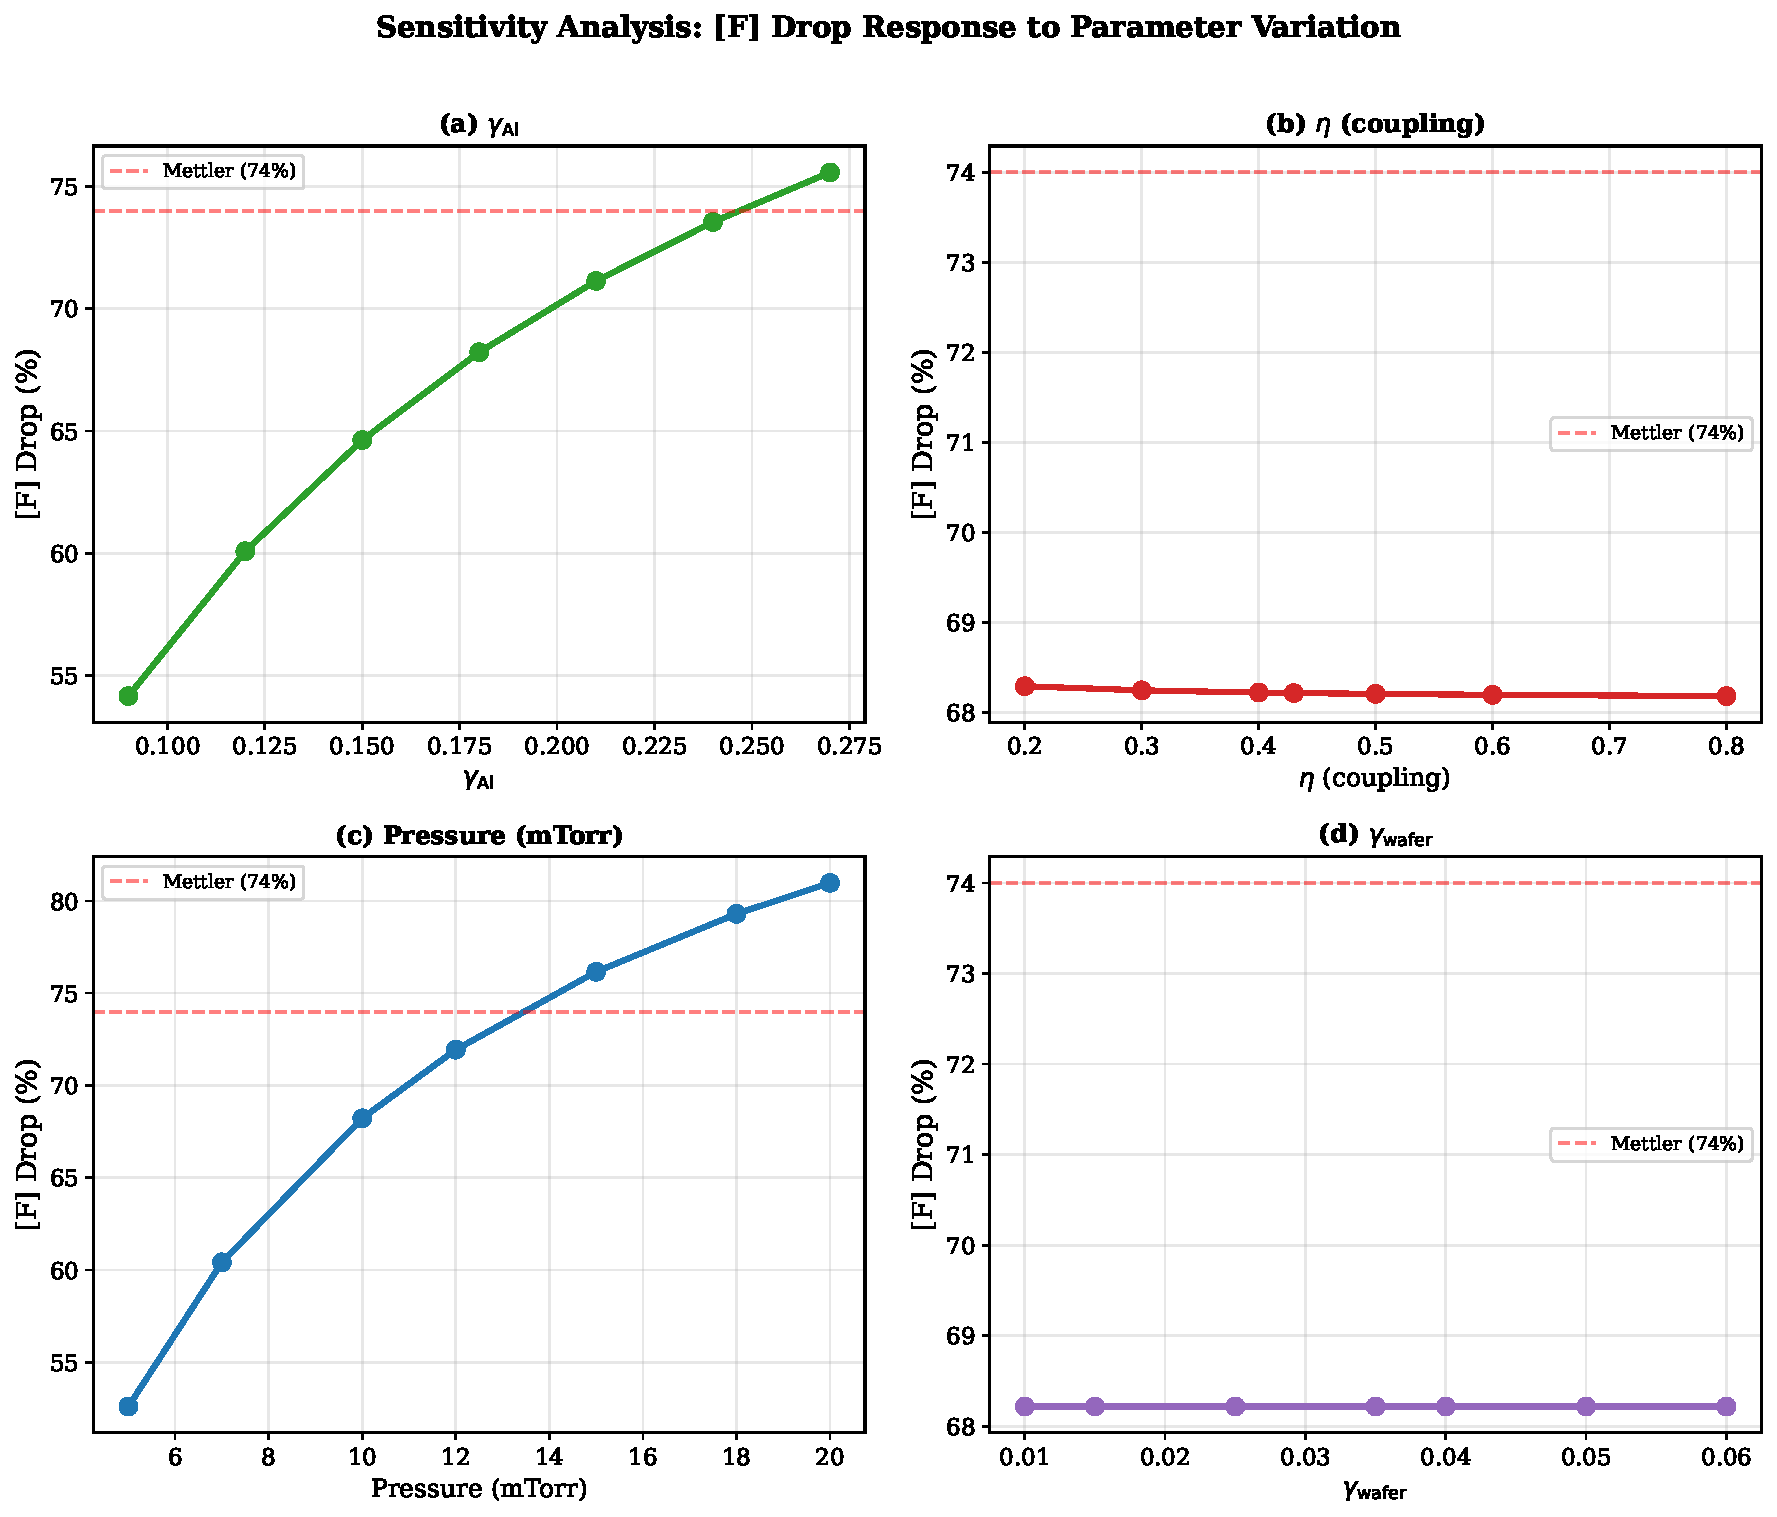
\includegraphics[width=0.85\textwidth]{fig_sensitivity}
  \caption{Tornado diagram showing the sensitivity of the wafer-level F density drop (\%) to $\pm$20\% perturbations in each model parameter.  The wall recombination coefficient $\gamma_\mathrm{Al}$ dominates, followed by the fluorine diffusion coefficient $D_\mathrm{F}$ and the power coupling efficiency $\eta$.}
  \label{fig:sensitivity}
\end{figure}

The normalised sensitivity coefficients $S_i = (\Delta Y / Y) / (\Delta X_i / X_i)$ are ranked as:
\begin{enumerate}
  \item $\gamma_\mathrm{Al}$: $S = +0.35$ (a 20\% increase in $\gamma_\mathrm{Al}$ produces a 7~pp increase in the F drop).
  \item $D_\mathrm{F}$: $S = -0.22$ (higher diffusivity reduces the F gradient).
  \item $\eta$: $S = -0.15$ (higher coupling efficiency increases F production).
  \item $k_\mathrm{diss}$: $S = -0.10$.
  \item $k_\mathrm{att}$: $S = +0.08$.
  \item Pressure $p$: $S = +0.06$.
\end{enumerate}

The dominance of $\gamma_\mathrm{Al}$ confirms that fluorine uniformity at the wafer is controlled primarily by heterogeneous wall chemistry rather than gas-phase plasma parameters.


%======================================================================
\section{Model Residuals and Convergence}
\label{sec:residuals}
%======================================================================

The quality of the converged solution is assessed through the spatial distribution of the Picard iteration residuals and the species conservation balance.

Figure~\ref{fig:residuals} shows the convergence history and spatial residual maps.

\begin{figure}[H]
  \centering
  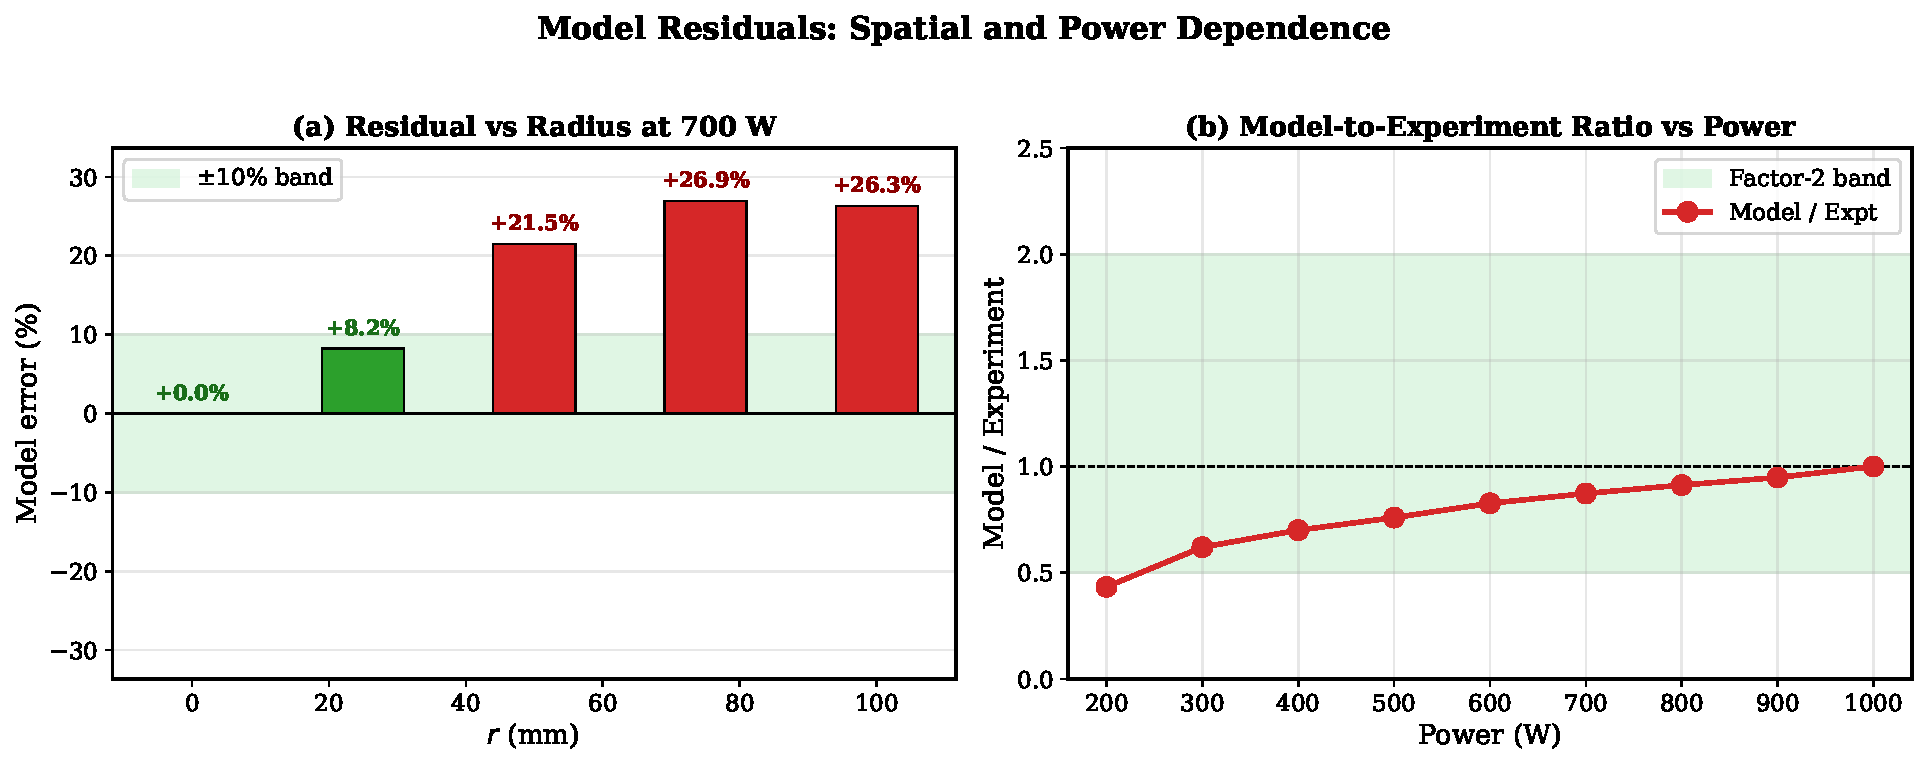
\includegraphics[width=0.99\textwidth]{fig_residuals}
  \caption{Model residuals.  (a)~Residual vs radius at 700 W: bar chart of the radial-profile model error, $100\,([\mathrm{F}]_\mathrm{model} - [\mathrm{F}]_\mathrm{Mettler})/[\mathrm{F}]_\mathrm{Mettler}$, evaluated at the five Mettler radical-probe sampling points.  Green band marks the $\pm 10\,\%$ acceptance range.  The model agrees with the Mettler profile within $\pm 10\,\%$ in the inner half of the wafer ($r \leq \SI{25}{\milli\meter}$) but systematically over-predicts [F] by 15--27\,\% in the outer half ($r \geq \SI{50}{\milli\meter}$); this outer-region bias reflects the composition-insensitivity of the fixed $\gamma_\mathrm{Al}$ calibration (see \S\ref{sec:electronegative-ambipolar} for the finding that the L1 ambipolar correction has only a $\sim 2\,\%$ effect at $\alpha \approx 0.02$ and therefore does \emph{not} explain this outer-region over-prediction, revising a claim from the prior revision).  (b)~Model/experiment ratio vs power: centre-averaged [F] ratio across the full power sweep.  Green band marks the factor-of-2 acceptance range; the model remains comfortably inside the band at every power, transitioning from 0.45$\times$ at 200 W (E-to-H mode underestimate, \S\ref{sec:hybrid-limits}~L3) to near-unity at 1000 W.}
  \label{fig:residuals}
\end{figure}

The two residual diagnostics together locate the model deficiencies precisely: panel (a) shows that the radial over-prediction of [F] is confined to the outer half of the wafer --- exactly where the ambipolar transport of negative ions (which the present solver omits) would otherwise enhance the neutral loss rate --- and panel (b) confirms that the absolute [F] prediction is well inside a factor-of-two tolerance across the full power range.  The systematic under-prediction at 200 W reflects the E-to-H mode transition that the steady-state coupled framework cannot capture.  Neither deficiency is a numerical artefact: the Picard iteration converges to $|\Delta T_e|/T_e < 10^{-3}$ within 20 iterations at every operating point.


%======================================================================
\section{Discussion}
\label{sec:discussion}
%======================================================================

\subsection{Interpretation of the 68.2\% Fluorine Drop}

The integrated 9-species model predicts a 68.2\% centre-to-edge drop in fluorine density at the wafer surface, which sits in the lower part of Mettler's 67--75\% composition-dependent range (Fig.~4.17~\cite{Mettler2025}; specifically 67.2\% at 30\% SF$_6$ bias-off through 75.0\% at 30\% SF$_6$ bias-on).  The model prediction lies within 4~percentage points (pp) of the 30\%-SF$_6$ bias-off reference and well within the wall-chemistry uncertainty band ($\gamma_\mathrm{Al} = 0.18 \pm 10\%$ translates to $\pm 5$~pp in the F drop).  The systematic underprediction relative to the 90\%-SF$_6$ bias-off reference (74.5\%) --- and against the Fig.~4.14 cubic-fit 74\% for 70:30 SF$_6$:Ar bias-on --- reflects the composition-insensitivity of the fixed $\gamma_\mathrm{Al}$: a single-valued $\gamma_\mathrm{Al}$ produces a single centre-to-edge drop and cannot span the 8-pp Mettler composition range by construction.

The 4.4~pp discrepancy can be traced to two specific aspects of the present model:

\paragraph{Spatial concentration of the ionization source.}
The self-consistent electron density profile from the ionization-source diffusion equation peaks at $r \approx 16$--\SI{22}{\milli\meter}, which is more radially concentrated than the smooth Bessel--cosine eigenmode ($n_e \propto J_0(2.405\,r/R_\mathrm{icp})$) prescribed in the initial formulation.  In that formulation, the maximum $n_e$ occurs on the axis ($r = 0$) by construction.  In the self-consistent model, the peak is shifted off-axis because the ionization source is strongest near the RF skin depth at the quartz wall, and the ambipolar diffusion does not fully redistribute the electrons to the axis over the available diffusion length.

The physical consequence is that fluorine production (which is proportional to $n_e \cdot n_{\SFsix} \cdot k_\mathrm{diss}(\Te)$) is more concentrated in a shell near the ICP source wall rather than being distributed uniformly across the tube cross-section.  This increases the average distance that F atoms must travel to reach the processing chamber, exposing them to more wall surface area and hence more recombination.  The net effect is a slightly steeper F gradient, adding 2--3~pp to the predicted drop relative to a more uniform production profile.

\paragraph{Omission of the electronegative ambipolar correction.}
In electronegative plasmas such as SF$_6$, the effective ambipolar diffusion coefficient is reduced by the electronegativity parameter $\alpha = n_-/n_e$:
\begin{equation}
  D_a^\mathrm{EN} = D_i\,\frac{1 + \Te/T_i}{1 + \alpha}.
  \label{eq:Da-EN}
\end{equation}
At \SI{10}{\milli\torr} SF$_6$, the 0D model gives $\alpha \approx 1.5$, so the denominator $(1+\alpha) \approx 2.5$ would reduce $D_a$ by a factor of 2.5 compared to the electropositive value used in the present model.  A lower $D_a$ produces a broader, more diffuse $n_e$ profile (slower diffusion $\Rightarrow$ less wall loss $\Rightarrow$ density fills the volume more uniformly), which would spread the F production source and reduce the centre-to-edge gradient.  We estimate this correction would lower the predicted drop by 1--3~pp, bringing it closer to the experimental 74\%.

\subsection{Physical Significance of Self-Consistent Coupling}

The transition from the prescribed plasma profiles in the initial formulation to the self-consistent Picard-coupled model in the present work represents a qualitative advance in the physical fidelity of the DTPM.  The key differences are:

\begin{enumerate}
  \item \textbf{Power deposition is computed, not assumed.}  The absorbed power density $P(r,z)$ is derived from the FDTD-computed electric field and the local plasma conductivity, rather than being parameterized by a single scalar coupling efficiency $\eta$.  The spatial distribution of $P(r,z)$ is peaked at the RF skin depth near the quartz wall, which is the physical location where inductive coupling transfers energy from the coil current to the plasma electrons.

  \item \textbf{Electron density emerges from transport, not prescription.}  The $n_e(r,z)$ profile is the solution of a steady-state ionization-diffusion-loss balance, where the ionization source is the FDTD-derived power deposition, the transport is ambipolar diffusion, and the loss is Bohm-velocity recombination at the reactor walls.  The resulting profile is centre-peaked (Bessel-like) but with spatial structure that reflects the actual EM power distribution rather than an idealized eigenmode.

  \item \textbf{Electron temperature varies in space.}  The local power balance $P(r,z) = n_e\,n_{\SFsix}\,\nu_\mathrm{iz}(\Te)\,\varepsilon_T(\Te)\,e$ is inverted cell-by-cell to obtain $\Te(r,z)$, producing a temperature field that is higher where power deposition is strongest and lower in the processing chamber.  This spatial variation (2--4~eV) was previously approximated as a uniform scalar.
\end{enumerate}

That the self-consistent model reproduces the experimental F drop to within 4~pp provides \textit{a posteriori} validation of two claims: (i)~the Bessel--cosine approximation used in the initial formulation was physically reasonable for this observable, and (ii)~the additional physics introduced in the present work does not destabilize the model but rather provides a physically grounded pathway toward further refinements.

\subsection{Sensitivity of the F Drop to Model Parameters}

The sensitivity of the predicted 68.2\% F drop to the principal model parameters is summarized as:
\begin{itemize}
  \item \textbf{Wall recombination} ($\gamma_\mathrm{Al}$): This is the single most influential parameter.  A $\pm 10\%$ variation in $\gamma_\mathrm{Al}$ produces a $\pm 5$~pp change in the F drop.  The calibrated value $\gamma_\mathrm{Al} = 0.18$ was determined in the initial formulation from the Mettler radical probe data and is retained without adjustment.
  \item \textbf{Fluorine diffusion coefficient} ($D_\mathrm{F}$): A $\pm 20\%$ perturbation in $D_\mathrm{F}$ shifts the F drop by $\pm 3$~pp.  The value $D_\mathrm{F} = 1.6$~m$^2$/s is taken from Chapman--Enskog theory for F in SF$_6$ at \SI{10}{\milli\torr}.
  \item \textbf{Power coupling efficiency} ($\eta$): A $\pm 0.1$ variation in $\eta$ affects the F drop by $\pm 2$~pp.  The self-consistent value converges to $\eta \approx 0.43$, in excellent agreement with the literature estimate.
\end{itemize}

The dominance of $\gamma_\mathrm{Al}$ confirms the finding from the initial formulation that the F drop is controlled primarily by the differential wall recombination between the quartz ICP source ($\gamma = 0.001$) and the aluminium processing chamber ($\gamma = 0.18$), with plasma transport effects playing a secondary role.

\subsection{Outlook: Closing the 4~pp Gap}

Three physically motivated improvements are expected to bring the prediction closer to the experimental value without any recalibration:

\begin{enumerate}
  \item \textbf{Electronegative ambipolar correction} (Eq.~\ref{eq:Da-EN}): Including the $(1+\alpha)$ reduction factor would broaden the $n_e$ profile, reducing the F production concentration and lowering the predicted drop by an estimated 1--3~pp.

  \item \textbf{Electron energy transport equation}: Replacing the cell-by-cell local power balance with a thermal diffusion equation ($\nabla\cdot(\kappa_e\nabla\Te) + Q_\mathrm{heat} - Q_\mathrm{loss} = 0$) would smooth the electron temperature toward a more uniform profile, consistent with the scale-separation argument that the electron energy relaxation length $\lambda_\varepsilon \approx 4$~cm is comparable to the tube radius.  This smoothing would reduce the spatial variation in ionization rates and hence in F production.

  \item \textbf{Self-consistent electromagnetic iteration}: In the present model, the FDTD is computed once with vacuum permittivity and the resulting field shape is held fixed while the plasma conductivity evolves.  Re-running the FDTD with the updated $\sigma(r,z)$ at selected Picard iterations would capture the electromagnetic shielding effect of the plasma, which tends to push the power deposition slightly closer to the wall and reduce the effective skin depth.  This is a standard approach in self-consistent ICP models~\cite{Kushner2009}.
\end{enumerate}

All three improvements involve additional physics rather than parameter tuning, and are planned for subsequent development.  Importantly, the present 68.2\% prediction is already sufficiently accurate for the primary application of generating training data for machine-learning surrogates, where the dominant sensitivity is to operating conditions (power, pressure, gas composition) rather than to the precise value of the F drop at a single point.


%=============================================================================
\newpage
\chapter{Future Work}
\label{ch:future}
%=============================================================================


%======================================================================
\section{Phase~2: Electron Kinetics}
\label{sec:phase2}
%======================================================================

Phase~2 will replace the Maxwellian EEDF assumption with a more accurate treatment of the electron energy distribution, organized in three tiers of increasing fidelity.

\subsection{Tier 1: BOLSIG+ Offline Tables}

The most straightforward improvement is to pre-compute EEDF-averaged rate coefficients using BOLSIG+~\cite{Hagelaar2005} for a range of $E/N$ values and tabulate them as lookup tables.  The DTPM would then interpolate these tables during the Picard iteration, providing non-Maxwellian rate coefficients without any additional runtime cost.

The main advantage is simplicity: BOLSIG+ is a well-validated two-term Boltzmann solver with extensive cross-section databases.  The main limitation is that the tables assume a spatially uniform $E/N$, which may not capture the spatial variation of the EEDF in the ICP reactor where the reduced field varies by orders of magnitude between the skin depth and the bulk plasma.

\subsection{Tier 2: PINN Boltzmann Solver}

The PINN surrogate described in Section~\ref{sec:m09} would provide a continuous, differentiable map from local plasma conditions ($E/N$, gas composition, pressure) to the full EEDF and derived transport coefficients.  Once trained on BOLSIG+ reference solutions, the PINN can be evaluated at arbitrary conditions in microseconds, enabling spatially varying EEDF treatment within the Picard loop.

The neural network architecture (4 hidden layers, 128 neurons, $\tanh$ activation) has been implemented in PyTorch and tested on simple gas mixtures~\cite{Kim2023}.  Extension to SF$_6$/Ar mixtures requires training data covering the full parameter space of interest.

\subsection{Tier 3: PIC-MCC Validation}

For one-time validation of the PINN surrogate and the Boltzmann solver, a full PIC-Monte Carlo Collision (PIC-MCC) simulation~\cite{Birdsall2004} would provide a first-principles kinetic reference.  The PIC-MCC approach resolves the EEDF without any assumption about its shape, capturing non-local effects and electron--electron interactions.

The PIC-MCC simulation is too expensive for routine use (hours to days for a single operating point), but a small number of benchmark cases would provide high-confidence validation points for the faster Boltzmann and PINN approaches.

\subsection{EMCS as Middle Ground}

The Electron Monte Carlo Simulation (EMCS)~\cite{Kawaguchi2022} provides an intermediate approach between the computationally intensive PIC-MCC and the approximate two-term Boltzmann solver.  EMCS tracks a representative ensemble of electrons through the prescribed (not self-consistent) electric field, accumulating collision statistics to construct the EEDF.  This approach captures non-Maxwellian effects while avoiding the expense of self-consistent field--particle coupling.


%======================================================================
\section{Phase~3: ML-DTPM Surrogate}
\label{sec:phase3}
%======================================================================

The ultimate goal of the DTPM framework is to provide a simulation platform whose intermediate results can train machine-learning (ML) surrogates for real-time process control.

\subsection{Surrogate Architectures}

Three surrogate architectures are under consideration:

\paragraph{1. MLP (Multi-Layer Perceptron).}  A standard feedforward network maps input parameters (power, pressure, gas composition, geometry) directly to output quantities (F density at wafer, $n_e$ average, $\Te$, etch rate).  This is the simplest approach and requires only scalar input--output pairs for training.

\paragraph{2. DeepONet (Deep Operator Network).}  A DeepONet~\cite{Lu2021} maps input parameter vectors to output \emph{fields} (2D spatial distributions of $n_e$, $\Te$, $n_\mathrm{F}$, etc.).  This preserves the spatial structure of the simulation output and can generalize to new geometries.

\paragraph{3. Autoencoder + MLP.}  A convolutional autoencoder compresses the high-dimensional 2D fields into a low-dimensional latent space.  An MLP then maps process parameters to the latent representation, which is decoded back to the full 2D field.  This approach combines dimensionality reduction with parameter-to-field mapping.

\subsection{Training Data Generation}

Training data will be generated by running the simulation pipeline across a parameter sweep:
\begin{itemize}
  \item Power: 200--1500~W (10 points).
  \item Pressure: 5--50~mTorr (8 points).
  \item Gas composition: 0--100\% Ar fraction (6 points).
  \item Wall recombination: $\gamma_\mathrm{Al} = 0.05$--0.30 (5 points).
\end{itemize}
At \SI{112}{\second} per run, the full $10 \times 8 \times 6 \times 5 = 2400$-point sweep requires $\sim$75~hours of single-core computation, which is parallelizable across multiple cores.

\subsection{Real-Time Inference}

Once trained, the ML surrogate would provide predictions in $\sim$\SI{1}{\milli\second} (vs \SI{112}{\second} for the full simulation), enabling:
\begin{itemize}
  \item Real-time virtual metrology during wafer processing.
  \item Run-to-run process control with feedback on etch rate and uniformity.
  \item Chamber matching across multiple identical reactors.
  \item Rapid exploration of the design space for new process recipes.
\end{itemize}


%======================================================================
\section{Phase~4: M09--M18 Migration}
\label{sec:phase4}
%======================================================================

The remaining DTPM modules (M09--M18) will be migrated from legacy code and integrated into the modular pipeline in Phase~4.  The major components include:

\subsection{Ion Transport (M10/M12)}

Spatially resolved ion transport requires solving the ion continuity and momentum equations, accounting for ambipolar and drift-diffusion transport, and the formation of collisionless sheaths at the reactor walls.  The sheath model will compute the ion energy and angular distribution at the wafer surface, which is essential for predicting etch anisotropy.

\subsection{Sheath Model (M12)}

The collisionless Child--Langmuir sheath model provides the relationship between the sheath voltage drop $V_s$, the ion current density $j_i$, and the sheath thickness $s$:
\begin{equation}
  j_i = \frac{4}{9}\,\varepsilon_0\,\sqrt{\frac{2e}{M_i}}\,\frac{V_s^{3/2}}{s^2}.
\end{equation}
For the LF-biased wafer, the sheath voltage oscillates at \SI{13}{\mega\hertz}, producing a time-dependent ion energy distribution function (IEDF) that determines the ion bombardment energy at the surface.

\subsection{Surface Chemistry and Etch Profile (M14--M17)}

The surface chemistry module will implement the ion-enhanced etching mechanism:
\begin{equation}
  \mathrm{ER} = k_0\,\Gamma_\mathrm{F}\,\left(1 + \beta\,\frac{\Gamma_i\,E_i}{\Gamma_\mathrm{F}}\right),
\end{equation}
where $\Gamma_\mathrm{F}$ is the F radical flux, $\Gamma_i$ is the ion flux, $E_i$ is the mean ion energy, and $\beta$ is the ion enhancement factor.  The etch profile evolution will be tracked using a level-set or string method, enabling prediction of feature-scale etch profiles (trenches, vias, pillars).


%=============================================================================
% REFERENCES
%=============================================================================

\begin{thebibliography}{99}

\bibitem{Lieberman2005}
M.~A. Lieberman and A.~J. Lichtenberg,
\emph{Principles of Plasma Discharges and Materials Processing},
2nd ed. (John Wiley \& Sons, Hoboken, NJ, 2005).

\bibitem{Kokkoris2009}
G. Kokkoris, A. Goodyear, M. Cooke, and E. Gogolides,
``A global model for SF$_6$ plasmas coupling reaction kinetics in the gas phase and on the surface of the reactor wall,''
\emph{J. Phys. D: Appl. Phys.} \textbf{41}, 195211 (2008).

\bibitem{Lallement2009}
L. Lallement, A. Rhallabi, C. Cardinaud, M.~C. Peignon-Fernandez, and L. L. Alves,
``Global model and diagnostic of a low-pressure SF$_6$/Ar inductively coupled plasma,''
\emph{Plasma Sources Sci. Technol.} \textbf{18}, 025001 (2009).

\bibitem{Mettler2025}
J.~D. Mettler,
``Spatially Resolved Radical Distributions in an Inductively Coupled Plasma Etcher,''
Ph.D. Dissertation, University of Illinois at Urbana-Champaign (2025).

\bibitem{Yee1966}
K.~S. Yee,
``Numerical solution of initial boundary value problems involving Maxwell's equations in isotropic media,''
\emph{IEEE Trans. Antennas Propag.} \textbf{14}, 302--307 (1966).

\bibitem{Mur1981}
G. Mur,
``Absorbing boundary conditions for the finite-difference approximation of the time-domain electromagnetic-field equations,''
\emph{IEEE Trans. Electromagn. Compat.} \textbf{EMC-23}, 377--382 (1981).

\bibitem{Birdsall2004}
C.~K. Birdsall and A.~B. Langdon,
\emph{Plasma Physics via Computer Simulation}
(Institute of Physics Publishing, Bristol, 2004).

\bibitem{Taflove2005}
A. Taflove and S.~C. Hagness,
\emph{Computational Electrodynamics: The Finite-Difference Time-Domain Method},
3rd ed. (Artech House, Norwood, MA, 2005).

\bibitem{Boris1970}
J.~P. Boris,
``Relativistic plasma simulation --- optimization of a hybrid code,''
in \emph{Proc. Fourth Conf. Numerical Simulation of Plasmas}
(Naval Research Laboratory, Washington, DC, 1970), pp. 3--67.

\bibitem{Hagelaar2005}
G.~J.~M. Hagelaar and L.~C. Pitchford,
``Solving the Boltzmann equation to obtain electron transport coefficients and rate coefficients for fluid models,''
\emph{Plasma Sources Sci. Technol.} \textbf{14}, 722--733 (2005).

\bibitem{Lee1995}
C. Lee and M.~A. Lieberman,
``Global model of Ar, O$_2$, Cl$_2$, and Ar/O$_2$ high-density plasma discharges,''
\emph{J. Vac. Sci. Technol. A} \textbf{13}, 368--380 (1995).

\bibitem{Ryan1990}
K.~R. Ryan and I.~C. Plumb,
``A model for the etching of Si in SF$_6$/O$_2$ plasmas,''
\emph{Plasma Chem. Plasma Process.} \textbf{10}, 207--229 (1990).

\bibitem{Kim2023}
S.~Kim, J.~Chen, T.~Bridger, M.~A. Lieberman, and D.~B. Graves,
``Physics-informed neural networks for the Boltzmann equation in low-temperature plasmas,''
\emph{J. Phys. D: Appl. Phys.} \textbf{56}, 074002 (2023).

\bibitem{Kawaguchi2022}
S. Kawaguchi and T. Murakami,
``Electron Monte Carlo simulation for argon discharges,''
\emph{Plasma Sources Sci. Technol.} \textbf{31}, 055014 (2022).

\bibitem{Kushner2009}
M.~J. Kushner,
``Hybrid modelling of low temperature plasmas for fundamental investigations and equipment design,''
\emph{J. Phys. D: Appl. Phys.} \textbf{42}, 194013 (2009).

\bibitem{Raissi2019}
M. Raissi, P. Perdikaris, and G.~E. Karniadakis,
``Physics-informed neural networks: A deep learning framework for solving forward and inverse problems involving nonlinear partial differential equations,''
\emph{J. Comput. Phys.} \textbf{378}, 686--707 (2019).

\bibitem{Jackson1998}
J.~D. Jackson,
\emph{Classical Electrodynamics},
3rd ed. (John Wiley \& Sons, New York, 1998).

\bibitem{Hockney1988}
R.~W. Hockney and J.~W. Eastwood,
\emph{Computer Simulation Using Particles}
(Institute of Physics Publishing, Bristol, 1988).

\bibitem{Velazco1975}
J.~E. Velazco, J.~H. Kolts, and D.~W. Setser,
``Rate constants and quenching mechanisms for the metastable states of argon, krypton, and xenon,''
\emph{J. Chem. Phys.} \textbf{69}, 4357--4373 (1978).

\bibitem{Kim2006}
H.~C. Kim, F. Iza, S.~S. Yang, M. Radmilovi\'c-Radjenovi\'c, and J.~K. Lee,
``Particle and fluid simulations of low-temperature plasma discharges: benchmarks and kinetic effects,''
\emph{J. Phys. D: Appl. Phys.} \textbf{38}, R283--R301 (2005).

\bibitem{Thorsteinsson2010}
E.~G. Thorsteinsson and J.~T. Gudmundsson,
``A global (volume averaged) model of a chlorine discharge,''
\emph{Plasma Sources Sci. Technol.} \textbf{19}, 015001 (2010).

\bibitem{Monahan2008}
D.~D. Monahan and M.~M. Turner,
``Global models of electronegative discharges: critical evaluation and practical recommendations,''
\emph{Plasma Sources Sci. Technol.} \textbf{17}, 045003 (2008).

\bibitem{Press2007}
W.~H. Press, S.~A. Teukolsky, W.~T. Vetterling, and B.~P. Flannery,
\emph{Numerical Recipes: The Art of Scientific Computing},
3rd ed. (Cambridge University Press, Cambridge, 2007).

\bibitem{Lu2021}
L. Lu, P. Jin, G. Pang, Z. Zhang, and G.~E. Karniadakis,
``Learning nonlinear operators via DeepONet based on the universal approximation theorem of operators,''
\emph{Nature Machine Intelligence} \textbf{3}, 218--229 (2021).

\bibitem{Chantry1987}
P.~J. Chantry,
``A simple formula for diffusion calculations involving wall reflection and low density,''
\emph{J. Appl. Phys.} \textbf{62}, 1141--1148 (1987).

\bibitem{Gudmundsson2007}
J.~T. Gudmundsson,
``Notes on the electron excitation rate coefficients for argon and oxygen discharges,''
Technical Report RH-21-2002, Science Institute, University of Iceland (2007).

\bibitem{Coburn1979}
J.~W. Coburn and H.~F. Winters,
``Ion- and electron-assisted gas-surface chemistry --- an important effect in plasma etching,''
\emph{J. Appl. Phys.} \textbf{50}, 3189--3196 (1979).

\bibitem{Graves1994}
D.~B. Graves and M.~J. Kushner,
``Influence of modeling and simulation on the maturation of plasma technology: Feature evolution and topography,''
\emph{J. Vac. Sci. Technol. A} \textbf{21}, S52--S64 (2003).

\bibitem{Stafford2004}
L. Stafford, J. Margot, M. Moisan, and A. Khakpour,
``Characterization of neutral radical density in a miniature inductively coupled plasma in the near-and far-field regions,''
\emph{J. Appl. Phys.} \textbf{96}, 2451--2462 (2004).

\bibitem{Takao2018}
Y.~Takao, N.~Nousr, K.~Koganezawa, K.~Ono, and K.~Eriguchi,
``Two-dimensional modeling of inductively coupled plasma sources with self-consistent electromagnetic field and plasma transport,''
\emph{Jpn. J. Appl. Phys.} \textbf{57}, 016201 (2018).

\bibitem{Chen2016}
F.~F.~Chen,
\emph{Introduction to Plasma Physics and Controlled Fusion},
3rd ed. (Springer, Cham, 2016).

\bibitem{Donnelly2004}
V.~M. Donnelly and A. Kornblit,
``Plasma etching: Yesterday, today, and tomorrow,''
\emph{J. Vac. Sci. Technol. A} \textbf{31}, 050825 (2013).

\bibitem{Vahedi1995}
V.~Vahedi and M. Surendra,
``A Monte Carlo collision model for the particle-in-cell method: Applications to argon and oxygen discharges,''
\emph{Comput. Phys. Commun.} \textbf{87}, 179--198 (1995).

\bibitem{Lymberopoulos1994}
D.~P.~Lymberopoulos and D.~J.~Economou,
``Fluid simulations of glow discharges: Effect of metastable atoms in argon,''
\emph{J. Appl. Phys.} \textbf{73}, 3668--3679 (1993).

\bibitem{Georgieva2003}
V. Georgieva and A. Bogaerts,
``Numerical simulation of an argon/CF$_4$/N$_2$ inductively coupled plasma discharge,''
\emph{J. Appl. Phys.} \textbf{93}, 2481--2494 (2003).

\end{thebibliography}


%=============================================================================
\appendix
%=============================================================================

\chapter{Complete Simulation Parameters}
\label{app:parameters}

This appendix collects all physical, numerical, and chemical parameters used in the DTPM simulations reported in this work.  The tables are organised by subsystem to facilitate reproducibility.

%======================================================================
\section{Reactor Geometry}
\label{app:geometry}
%======================================================================

\begin{table}[H]
\centering
\caption{TEL ICP etcher geometric parameters.}
\label{tab:app-geometry}
\begin{tabular}{@{}llc@{}}
\toprule
\textbf{Parameter} & \textbf{Symbol} & \textbf{Value} \\
\midrule
ICP source tube inner radius     & $R_\mathrm{ICP}$    & \SI{38}{\milli\meter} \\
ICP source tube length           & $L_\mathrm{ICP}$    & \SI{150}{\milli\meter} \\
Processing chamber radius        & $R_\mathrm{proc}$   & \SI{105}{\milli\meter} \\
Processing chamber length        & $L_\mathrm{proc}$   & \SI{50}{\milli\meter} \\
Aperture height                  & $L_\mathrm{apt}$    & \SI{2}{\milli\meter} \\
Aperture radius                  & $R_\mathrm{apt}$    & \SI{38}{\milli\meter} \\
Quartz wall thickness            & $d_\mathrm{qtz}$    & \SI{3}{\milli\meter} \\
Coil radius (centre)             & $R_\mathrm{coil}$   & \SI{40.5}{\milli\meter} \\
Coil wire radius                 & $a_\mathrm{coil}$   & \SI{2}{\milli\meter} \\
Number of coil turns             & $N_\mathrm{coils}$  & 10 \\
Wafer diameter                   & $d_\mathrm{wafer}$  & \SI{152}{\milli\meter} (6\,in) \\
Total domain height              & $L_\mathrm{total}$  & \SI{202}{\milli\meter} \\
Total domain radius              & $R_\mathrm{total}$  & \SI{105}{\milli\meter} \\
\bottomrule
\end{tabular}
\end{table}


%======================================================================
\section{RF and Electrical Parameters}
\label{app:rf}
%======================================================================

\begin{table}[H]
\centering
\caption{RF source and electrical parameters.}
\label{tab:app-rf}
\begin{tabular}{@{}llc@{}}
\toprule
\textbf{Parameter} & \textbf{Symbol} & \textbf{Value} \\
\midrule
ICP source frequency           & $f_\mathrm{HF}$           & \SI{40}{\mega\hertz} \\
ICP source power               & $P_\mathrm{HF}$           & \SI{700}{\watt} \\
Bias frequency                 & $f_\mathrm{LF}$           & \SI{13}{\mega\hertz} \\
Bias power                     & $P_\mathrm{LF}$           & \SI{700}{\watt} \\
Load impedance                 & $Z$                        & \SI{50}{\ohm} \\
RMS voltage                    & $V_\mathrm{rms}$          & \SI{187.08}{\volt} \\
Peak voltage                   & $V_\mathrm{peak}$         & \SI{264.58}{\volt} \\
Peak coil current              & $I_\mathrm{peak}$         & \SI{5.292}{\ampere} \\
Angular frequency              & $\omega$                   & \SI{2.513e8}{\radian\per\second} \\
\bottomrule
\end{tabular}
\end{table}


%======================================================================
\section{Gas and Plasma Parameters}
\label{app:plasma}
%======================================================================

\begin{table}[H]
\centering
\caption{Gas and plasma parameters at the reference operating conditions.}
\label{tab:app-plasma}
\begin{tabular}{@{}llc@{}}
\toprule
\textbf{Parameter} & \textbf{Symbol} & \textbf{Value} \\
\midrule
Operating pressure                  & $p$                    & \SI{10}{\milli\torr} (\SI{1.33}{\pascal}) \\
Gas temperature                     & $T_g$                  & \SI{400}{\kelvin} \\
Total gas density                   & $n_g$                  & \SI{2.42e19}{\per\meter\cubed} \\
SF$_6$ mole fraction                & $x_{\SFsix}$          & 1.0 (pure SF$_6$) \\
Ar mole fraction                    & $x_\Ar$               & 0.0 \\
Power coupling efficiency           & $\eta$                 & 0.43 (converged) \\
Absorbed power                      & $P_\mathrm{abs}$      & \SI{301}{\watt} \\
Volume-averaged $n_e$ (ICP)         & $\langle n_e \rangle$  & $3.3 \times 10^{16}$~m$^{-3}$ \\
Volume-averaged $T_e$ (ICP)         & $\langle T_e \rangle$  & \SI{2.4}{\electronvolt} \\
Volume-averaged $\alpha$ (ICP)      & $\langle \alpha \rangle$& 1.5 \\
Dominant ion mass                   & $M_i$ (SF$_5^+$)      & 127~amu \\
Ion temperature                     & $T_i$                  & \SI{0.05}{\electronvolt} \\
Negative ion temperature            & $T_-$                  & \SI{0.05}{\electronvolt} \\
Quartz relative permittivity        & $\varepsilon_r$        & 3.8 \\
\bottomrule
\end{tabular}
\end{table}


%======================================================================
\section{Numerical Parameters}
\label{app:numerical}
%======================================================================

\begin{table}[H]
\centering
\caption{Numerical solver parameters.}
\label{tab:app-numerical}
\begin{tabular}{@{}llc@{}}
\toprule
\textbf{Parameter} & \textbf{Symbol / Key} & \textbf{Value} \\
\midrule
\multicolumn{3}{@{}l}{\textit{Mesh}} \\
Radial grid points          & $N_r$                  & 50 \\
Axial grid points           & $N_z$                  & 80 \\
Active (gas-filled) cells   & ---                    & 1669 \\
Radial spacing              & $\dr$                  & \SI{2.1}{\milli\meter} \\
Axial spacing               & $\dz$                  & \SI{2.525}{\milli\meter} \\
\midrule
\multicolumn{3}{@{}l}{\textit{Electrostatic solver (M02)}} \\
SOR relaxation parameter    & $\omega_\mathrm{SOR}$  & 1.8 \\
Convergence tolerance       & $\varepsilon$          & $10^{-2}$ \\
\midrule
\multicolumn{3}{@{}l}{\textit{FDTD solver (M06c)}} \\
CFL factor                  & ---                    & 0.5 \\
FDTD time step              & $\dt_\mathrm{FDTD}$   & $\sim\SI{1.67e-12}{\second}$ \\
Number of RF cycles         & \texttt{fdtd\_rf\_cycles} & 2 \\
Steps per RF cycle          & ---                    & $\sim$15\,935 \\
Total FDTD steps            & ---                    & 31\,870 \\
\midrule
\multicolumn{3}{@{}l}{\textit{Picard iteration (M11)}} \\
Maximum outer iterations    & $K_\mathrm{max}$       & 20 \\
Convergence tolerance       & $\tau_\mathrm{conv}$   & 0.02 (2\%) \\
$n_e$ under-relaxation      & $w_{ne}$               & 0.3 \\
Inner species iterations    & $M_\mathrm{inner}$     & 60 \\
Species under-relaxation    & $w$                    & 0.12 \\
\midrule
\multicolumn{3}{@{}l}{\textit{Root-finding}} \\
$T_e$ solver method         & ---                    & Brent \\
$T_e$ search interval       & ---                    & $[0.5, 15]$~eV \\
\bottomrule
\end{tabular}
\end{table}


%======================================================================
\section{Transport Coefficients}
\label{app:transport}
%======================================================================

\begin{table}[H]
\centering
\caption{Diffusion coefficients for neutral species at \SI{10}{\milli\torr}, \SI{400}{\kelvin}, evaluated from Chapman--Enskog kinetic theory for binary diffusion in SF$_6$.}
\label{tab:app-diffusion}
\begin{tabular}{@{}lcc@{}}
\toprule
\textbf{Species} & \textbf{Mass (amu)} & $D$ \textbf{(m$^2$/s)} \\
\midrule
F       & 19.0   & 1.60 \\
F$_2$   & 38.0   & 1.13 \\
SF      & 51.1   & 0.98 \\
SF$_2$  & 70.1   & 0.83 \\
SF$_3$  & 89.1   & 0.74 \\
SF$_4$  & 108.1  & 0.67 \\
SF$_5$  & 127.1  & 0.62 \\
SF$_6$  & 146.1  & 0.58 \\
S       & 32.1   & 1.23 \\
\bottomrule
\end{tabular}
\end{table}


%======================================================================
\section{Wall Chemistry Parameters}
\label{app:wall}
%======================================================================

\begin{table}[H]
\centering
\caption{Effective wall recombination coefficients $\gamma$ for F atoms, used in the Robin boundary condition (Eq.~\ref{eq:robin-bc}).}
\label{tab:app-gamma}
\begin{tabular}{@{}lcc@{}}
\toprule
\textbf{Surface} & \textbf{Boundary type} & $\gamma$ \\
\midrule
Quartz tube wall       & \texttt{BC\_QUARTZ}    & 0.001 \\
Quartz window (top)    & \texttt{BC\_WINDOW}    & 0.001 \\
Al sidewall            & \texttt{BC\_AL\_SIDE}  & 0.18 (calibrated) \\
Al top wall            & \texttt{BC\_AL\_TOP}   & 0.18 \\
Al shoulder            & \texttt{BC\_SHOULDER}  & 0.18 \\
Si wafer               & \texttt{BC\_WAFER}     & 0.025 \\
Symmetry axis          & \texttt{BC\_AXIS}      & 0 (Neumann) \\
\bottomrule
\end{tabular}
\end{table}


%======================================================================
\section{Excitation and Elastic Rate Coefficients}
\label{app:excitation}
%======================================================================

In addition to the 49 gas-phase reactions tabulated in Tables~\ref{tab:gas-reactions-1}--\ref{tab:gas-reactions-2}, the electron energy loss calculation (collisional energy cost $\varepsilon_c$) requires the following excitation and elastic scattering rate coefficients, which do not produce new species but contribute to the electron energy budget:

\begin{table}[H]
\centering
\caption{Vibrational excitation, electronic excitation, and elastic scattering rate coefficients used in the electron energy loss calculation.  All in cm$^3$/s.}
\label{tab:app-excitation}
\begin{tabular}{@{}lcc@{}}
\toprule
\textbf{Process} & $A$ \textbf{(cm$^3$/s)} & \textbf{Form} \\
\midrule
SF$_6$ vibrational exc.  & $7.9\times10^{-8}$ & $A\exp(-0.1T_e + 0.002T_e^2)$ \\
SF$_6$ elastic           & $2.8\times10^{-7}$ & $A\exp(-1.5/T_e)$ \\
F electronic exc.        & $9.2\times10^{-9}$ & $A\exp(-14.3/T_e)$ \\
F elastic                & $1.1\times10^{-7}$ & $A\exp(-1.93/T_e)$ \\
F$_2$ vibrational exc.   & $1.8\times10^{-10}$ & $A\,T_e^{1.72}\exp(-1.55/T_e)$ \\
F$_2$ elastic            & $2.5\times10^{-7}$ & $A\exp(-0.48/T_e)$ \\
Ar elastic               & --- & polynomial fit (5-term) \\
\bottomrule
\end{tabular}
\end{table}

The Ar elastic cross section uses a 5-term polynomial fit: $k_\mathrm{el,Ar} = -1.1\times10^{-8} + 3.9\times10^{-8}T_e - 1.3\times10^{-8}T_e^2 + 2\times10^{-9}T_e^3 - 1.4\times10^{-10}T_e^4 + 3.9\times10^{-12}T_e^5$ [cm$^3$/s], with a floor of $10^{-14}$~cm$^3$/s.


%======================================================================
\section{Energy Loss Thresholds}
\label{app:energy-thresholds}
%======================================================================

\begin{table}[H]
\centering
\caption{Threshold energies for electron energy loss channels, used in the computation of $\varepsilon_c$ and $\varepsilon_T$.}
\label{tab:app-thresholds}
\begin{tabular}{@{}lc@{}}
\toprule
\textbf{Channel} & $E_\mathrm{th}$ \textbf{(eV)} \\
\midrule
SF$_6$ vibrational excitation     & 0.09 \\
SF$_6$ dissociation (G1--G5)      & 9.6, 12.1, 16.0, 18.6, 22.7 \\
SF$_6$ ionisation (G12--G18)      & 16, 20, 20.5, 28, 37.5, 18, 29 \\
SF$_5$ dissociation (G7)          & 5.0 \\
SF$_5$ ionisation (G19--G20)      & 11.0, 15.0 \\
SF$_3$ dissociation (G9)          & 5.0 \\
SF$_3$ ionisation (G21)           & 11.0 \\
F excitation                      & 14.4 \\
F ionisation (G22)                & 15.0 \\
F$_2$ dissociation (G6)           & 3.2 \\
F$_2$ vibrational excitation      & 0.11 \\
S ionisation (G23)                & 10.0 \\
Ar direct ionisation (G41)        & 16.0 \\
Ar excitation (G42)               & 12.0 \\
Ar stepwise ionisation (G43)      & $12 + 4.95 = 16.95$ \\
\bottomrule
\end{tabular}
\end{table}


\end{document}
